%% abtex2-modelo-trabalho-academico.tex, v-1.9.2 laurocesar
%% Copyright 2012-2014 by abnTeX2 group at http://abntex2.googlecode.com/
%%
%% This work may be distributed and/or modified under the
%% conditions of the LaTeX Project Public License, either version 1.3
%% of this license or (at your option) any later version.
%% The latest version of this license is in
%%   http://www.latex-project.org/lppl.txt
%% and version 1.3 or later is part of all distributions of LaTeX
%% version 2005/12/01 or later.
%%
%% This work has the LPPL maintenance status `maintained'.
%%
%% The Current Maintainer of this work is the abnTeX2 team, led
%% by Lauro César Araujo. Further information are available on
%% http://abntex2.googlecode.com/
%%
%% This work consists of the files abntex2-modelo-trabalho-academico.tex,
%% abntex2-modelo-include-comandos and abntex2-modelo-references.bib
%%

% ------------------------------------------------------------------------
% ------------------------------------------------------------------------
% abnTeX2: Modelo de Trabalho Academico (tese de doutorado, dissertacao de
% mestrado e trabalhos monograficos em geral) em conformidade com
% ABNT NBR 14724:2011: Informacao e documentacao - Trabalhos academicos -
% Apresentacao
% ------------------------------------------------------------------------
% ------------------------------------------------------------------------

\documentclass[
  % -- opções da classe memoir --
  12pt,        % tamanho da fonte
  openright,      % capítulos começam em pág ímpar (insere página vazia caso preciso)
  twoside,      % para impressão em verso e anverso. Oposto a oneside
  a4paper,      % tamanho do papel.
  % -- opções da classe abntex2 --
  %chapter=TITLE,    % títulos de capítulos convertidos em letras maiúsculas
  %section=TITLE,    % títulos de seções convertidos em letras maiúsculas
  %subsection=TITLE,  % títulos de subseções convertidos em letras maiúsculas
  %subsubsection=TITLE,% títulos de subsubseções convertidos em letras maiúsculas
  % -- opções do pacote babel --
  english,      % idioma adicional para hifenização
%  french,        % idioma adicional para hifenização
%  spanish,      % idioma adicional para hifenização
  brazil        % o último idioma é o principal do documento
]{abntex2}

% ---
% Pacotes básicos
% ---
\usepackage{lmodern}      % Usa a fonte Latin Modern
\usepackage[T1]{fontenc}    % Selecao de codigos de fonte.
\usepackage[utf8]{inputenc}    % Codificacao do documento (conversão automática dos acentos)
\usepackage[table,usenames,dvipsnames,xcdraw]{xcolor}     % para colorir céluas de tabelas
\usepackage{lastpage}      % Usado pela Ficha catalográfica
\usepackage{indentfirst}    % Indenta o primeiro parágrafo de cada seção.
%\usepackage[usenames,dvipsnames]{color}    % Controle das cores
\usepackage{graphicx}      % Inclusão de gráficos
\usepackage{microtype}       % para melhorias de justificação
\usepackage{soulutf8}          % usado para grifar textos com o comando '\hl{}'
\usepackage[portuguese,obeyFinal,textsize=tiny]{todonotes}         % Pacotes para inserir anotações de coisas a fazer
\usepackage{paralist}          % pacote usado para enumerações "em linha"
\usepackage{url}               % pacote para adicionar URLs no texto
\usepackage{epstopdf}
\usepackage{array}             % usado para centralizar células de tabelas
\usepackage{longtable}
\usepackage{pdflscape}         % usado para landscape de página
\usepackage{adjustbox}
\usepackage{booktabs}
\usepackage{varwidth}%
\usepackage{underscore}        % Para adicionar underscores nas urls
\usepackage[final]{pdfpages}          % Para fazer o include de arquivos PDF
\usepackage{amsmath}            % Para fórmulas matemáticas
\usepackage{longtable}     %para tabelas com mais de uma página
\usepackage{capa-epusp-abntex2}
\usepackage{multirow}
% ---

% ---
% Pacotes de citações
% ---
\usepackage[brazilian,hyperpageref]{backref}   % Paginas com as citações na bibl
\usepackage[alf]{abntex2cite}  % Citações padrão ABNT

\include{./personalizacoes/pacotes-configuracoes}

% ---
% Informações de dados para CAPA e FOLHA DE ROSTO
% ---
% Informações de dados para CAPA e FOLHA DE ROSTO
% ---
\titulo{Evolução dos padrões de deslocamento na Região Metropolitana de São Paulo: a necessidade de uma análise de gênero}
\autor{HAYD\'EE SVAB}
\local{São Paulo}
\data{2016}
\orientador[Orientador:]{Prof. Dr. Orlando Strambi}
\instituicao{%
  Universidade de São Paulo -- USP
  \par
  Escola Politécnica%
%  \par
%  Graduação em Engenharia Elétrica - Ênfase Computação  
  }
\tipotrabalho{Dissertação de Mestrado}
% O preambulo deve conter o tipo do trabalho, o objetivo,
% o nome da instituição e a área de concentração
\preambulo{Dissertação apresentada à Escola Politécnica da Universidade de São Paulo para obtenção do título de Mestre em Engenharia.}
\areaconcentracao{Planejamento de Transportes}
% ---
% ---

%\definecolor{lightblue}{rgb}{.80,.85,1}
%\definecolor{lightred}{rgb}{1,.80,.85}
%\definecolor{lightgreen}{rgb}{.80,1,.85}
%
%% COMANDOS PARA NOTAS DE "TODO"
%\newcounter{todocounter}
%%To-do que indica necessidade de correção de referência
%\newcommand{\corrigeref}[1]{
%    \sethlcolor{lightgreen}
%    #1\hl{(Corrigir referência)}\todonum[color=lightgreen]{Corrigir Referência}
%    \sethlcolor{yellow}
%}
%%To-do que destaca 'highlight' o texto e adiciona a nota também
%\newcommand{\todohl}[2]{
%    \hl{#1}\todonum{#2}
%}
%%To-do da cor vermelha, revisão do texto necessária
%\newcommand{\todorevisar}[1]{
%    \sethlcolor{lightred}
%    \hl{#1}\todonum[color=lightred]{Revisar o trecho}
%    \sethlcolor{yellow}
%}
%%To-do da cor azul, vindo de "Recorte e cole", possivelmente não vai ficar
%\newcommand{\todojogado}[1]{#1\todonum[color=blue!40]{Texto vindo de Recorte e Cole}}
%%To-do padrão numerado. Contém um parâmetro opcional para referência da localização da nota
%\newcommand{\todonum}[2][]{\stepcounter{todocounter}\todo[#1]{\thetodocounter: #2}}

%%%%%%%%%%%%%%%%%%%%%%%%%%%%%%%%%%%%%%%%%%%%%%%%%%%%%%%%%%%%%%%%%%%%%%%%%%%%%%%%%%%%%%%%%%%%%%%
% AMBIENTE E LISTA DE QUADROS
% Novo list of (listings) para QUADROS
\newcommand{\quadroname}{Quadro}
\newcommand{\listofquadrosname}{Lista de quadros}
\newfloat[chapter]{quadro}{loq}{\quadroname}
\newlistof{listofquadros}{loq}{\listofquadrosname}
\newlistentry{quadro}{loq}{0}

% configurações para atender às regras da ABNT
\counterwithout{quadro}{chapter}
\renewcommand{\cftquadroname}{\quadroname\space}
\renewcommand*{\cftquadroaftersnum}{\hfill--\hfill}


%%%%%%%%%%%%%%%%%%%%%%%%%%%%%%%%%%%%%%%%%%%%%%%%%%%%%%%%%%%%%%%%%%%%%%%%%%%%%%%%%%%%%%%%%%%%%%%
% AMBIENTE E LISTA DE GRÁFICOS
% Novo list of (listings) para GRÁFICOS
\newcommand{\graficoname}{Gr\'{a}fico}
\newcommand{\listofgraficosname}{Lista de gr\'{a}ficos}
\newfloat[chapter]{grafico}{lofg}{\graficoname}
\newlistof{listofgraficos}{lofg}{\listofgraficosname}
\newlistentry{grafico}{lofg}{0}

% configurações para atender às regras da ABNT
\counterwithout{grafico}{chapter}
\renewcommand{\cftgraficoname}{\graficoname\space}
\renewcommand*{\cftgraficoaftersnum}{\hfill--\hfill}

%%%%%%%%%%%%%%%%%%%%%%%%%%%%%%%%%%%%%%%%%%%%%%%%%%%%%%%%%%%%%%%%%%%%%%%%%%%%%%%%%%%%%%%%%%%%%%%




% Para centralizar células de tabelas
\newcolumntype{P}[1]{>{\centering\arraybackslash}p{#1}}
\newcolumntype{M}[1]{>{\centering\arraybackslash}m{#1}}

% Para rotacionar os títulos de forma adequada
\newcommand{\turn}[3][10em]{% \turn[<width>]{<angle>}{<stuff>}
  \rlap{\rotatebox[origin=rB]{#2}{\begin{varwidth}[t]{#1}\bfseries#3\end{varwidth}}}%
}

% Comandos de cores de céluas
%%Cor Padrão de cabeçalhos de tabelas
\newcommand{\headerColor}{RoyalBlue!95!black!20}
\newcommand{\headerFontStyle}{\sffamily\bfseries\color{white}}
\newcommand{\headerCell}[1]{
    %\multicolumn{1}{c|}{\cellcolor{\headerColor}\textcolor{white}{\sffamily\bfseries{#1}}}
    %\cellcolor{\headerColor}\textcolor{white}{\sffamily\bfseries{#1}}
    \textbf{#1}
}

\newcommand{\destValCel}[1]{\mbox{\color{Red!99!black!99}#1}}

\newcommand{\headerCenterCell}[1]{
    %\multicolumn{1}{c|}{\cellcolor{\headerColor}\textcolor{white}{\sffamily\bfseries{#1}}}
    %\cellcolor{\headerColor}\textcolor{white}{\sffamily\bfseries{#1}}
    \begin{center}\textbf{#1}\end{center}
}

\newcommand{\headerCenter}[3]{%
    %#1 = Qtde de Células
    %#2 = tamanho da célula
    %#2 = conteúdo
    \multicolumn{#1}{P{#2}}{\textbf{#3}}%
}%

\newcommand{\CellCenter}[3]{%
    %#1 = Qtde de Células
    %#2 = tamanho da célula
    %#2 = conteúdo
    \multicolumn{#1}{P{#2}}{#3}%
}%

\newcommand{\headerCenterM}[3]{%
    %#1 = Qtde de Células
    %#2 = tamanho da célula
    %#2 = conteúdo
  \multicolumn{#1}{|M{#2}}{{\headerCenterCell{\textbf{#3}}}}%
}%

\newcommand{\headerTabCenterCell}[1]{
    \multicolumn{1}{c}{\textbf{#1}}
}
\newcommand{\celAlinhaEsquerda}[1]{
    \multicolumn{1}{l}{#1}
}
\newcommand{\celAlinhaDireita}[1]{
    \multicolumn{1}{r}{#1}
}
\newcommand{\celAlinhaCentro}[1]{
    \multicolumn{1}{c}{#1}
}
\newcommand{\destaqueCel}{
    \cellcolor{\headerColor}
}
\newcommand{\quebraLinhaCel}[2][c]{%
  \begin{tabular}[#1]{@{}c@{}}#2\end{tabular}
}


%%%%%%%%%%%%%%%%%%%%%%%%%%%%%%%%%%%%%%%%%%%%%%%%%%%%%%%%%%%%%%%%%%%%%%%%%%%%%%%%%%%%%%%%%%%%%%%
% Refazendo comando de capa e folha de rosto
%\renewcommand{\imprimircapa}{%
%  \begin{capa}%
%    \center
%    
%    \imprimirinstituicao
%
%    \ABNTEXchapterfont\large\imprimirautor
%
%    \vfill
%    \ABNTEXchapterfont\bfseries\LARGE\imprimirtitulo
%    \vfill
%
%    \large\imprimirlocal
%
%    \large\imprimirdata
%
%    \vspace*{1cm}
%  \end{capa}
%}
%
%\renewcommand{\folhaderostocontent}{
%    \begin{center}
%
%      %\vspace*{1cm}
%      %\imprimirinstituicao
%
%      {\ABNTEXchapterfont\large\imprimirautor}
%
%      \vspace*{\fill}\vspace*{\fill}
%      \begin{center}
%      \ABNTEXchapterfont\bfseries\Large\imprimirtitulo
%      \end{center}
%      \vspace*{\fill}
%
%      \hspace{.45\textwidth}
%      \begin{minipage}{.5\textwidth}
%      \SingleSpacing
%      \imprimirpreambulo
%      \end{minipage}%
%      \vspace*{\fill}
%
%      {\large\imprimirorientadorRotulo~\imprimirorientador\par}
%      \large\imprimircoorientadorRotulo~\imprimircoorientador
%      \vspace*{\fill}
%
%      {\large\imprimirlocal}
%      \par
%      {\large\imprimirdata}
%      \vspace*{1cm}
%
%    \end{center}
%  }


% ---
% Configurações de aparência do PDF final

% alterando o aspecto da cor azul
\definecolor{blue}{RGB}{41,5,195}

% informações do PDF
\makeatletter
\hypersetup{
    %pagebackref=true,
    pdftitle={\@title},
    pdfauthor={\@author},
    pdfsubject={\imprimirpreambulo},
    pdfcreator={PDFLaTeX with abnTeX2},
    pdfkeywords={gênero}{transporte}{planejamento}{sustentabilidade}{mobilidade},
    colorlinks=true,           % false: boxed links; true: colored links
    linkcolor=blue,            % color of internal links
    citecolor=blue,            % color of links to bibliography
    filecolor=magenta,          % color of file links
    urlcolor=blue,
    bookmarksdepth=4
}
\makeatother
% ---

% ---
% Espaçamentos entre linhas e parágrafos
% ---

% O tamanho do parágrafo é dado por:
\setlength{\parindent}{1.3cm}

% Controle do espaçamento entre um parágrafo e outro:
\setlength{\parskip}{0.2cm}  % tente também \onelineskip

% ---
% compila o indice
% ---
\makeindex
% ---

% ----
% Início do documento
% ----
\begin{document}
%\stepcounter{chapter}

% Retira espaço extra obsoleto entre as frases.
\frenchspacing

% ----------------------------------------------------------
% ELEMENTOS PRÉ-TEXTUAIS
% ----------------------------------------------------------
% \pretextual

% ---
% Capa
% ---
\imprimircapa
% ---

% ---
% Folha de rosto
% (o * indica que haverá a ficha bibliográfica)
% ---
\imprimirfolhaderosto*
% ---

% ---
% Inserir a ficha bibliografica
% ---

% Isto é um exemplo de Ficha Catalográfica, ou ``Dados internacionais de
% catalogação-na-publicação''. Você pode utilizar este modelo como referência.
% Porém, provavelmente a biblioteca da sua universidade lhe fornecerá um PDF
% com a ficha catalográfica definitiva após a defesa do trabalho. Quando estiver
% com o documento, salve-o como PDF no diretório do seu projeto e substitua todo
% o conteúdo de implementação deste arquivo pelo comando abaixo:
%
% \begin{fichacatalografica}
%     \includepdf{fig_ficha_catalografica.pdf}
% \end{fichacatalografica}
%\begin{fichacatalografica}
%  \vspace*{\fill}          % Posição vertical
%  \hrule              % Linha horizontal
%  \begin{center}          % Minipage Centralizado
%  \begin{minipage}[c]{12.5cm}    % Largura
%
%  \imprimirautor
%
%  \hspace{0.5cm} \imprimirtitulo  / \imprimirautor. --
%  \imprimirlocal, \imprimirdata-
%
%  \hspace{0.5cm} \pageref{LastPage} p. : il. (algumas color.) ; 30 cm.\\
%
%  \hspace{0.5cm} \imprimirorientadorRotulo~\imprimirorientador\\
%
%%  \hspace{0.5cm} \imprimircoorientadorRotulo~\imprimircoorientador\\
%
%  \hspace{0.5cm}
%  \parbox[t]{\textwidth}{\imprimirtipotrabalho~--~\imprimirinstituicao,
%  \imprimirdata.}\\
%
%  \hspace{0.5cm} 
%    1. Planejamento de Transportes.
%    2. Análise de Demanda.
%    3. Gênero.
%    I. \imprimirorientadorRotulo~\imprimirorientador~
%    II. Universidade de São Paulo.
%    III. Escola Politécnica.
%    IV. Título\\
%
%  \hspace{8.75cm} CDU XX:XXX:XXX.X\\ %TODO
%
%  \end{minipage}
%  \end{center}
%  \hrule
%\end{fichacatalografica}
%% ---

% ---
% Inserir errata
% ---

%\begin{errata}
%Elemento opcional da \citeonline[4.2.1.2]{NBR14724:2011}. Exemplo:
%
%\vspace{\onelineskip}
%
%FERRIGNO, C. R. A. \textbf{Tratamento de neoplasias ósseas apendiculares com
%reimplantação de enxerto ósseo autólogo autoclavado associado ao plasma
%rico em plaquetas}: estudo crítico na cirurgia de preservação de membro em
%cães. 2011. 128 f. Tese (Livre-Docência) - Faculdade de Medicina Veterinária e
%Zootecnia, Universidade de São Paulo, São Paulo, 2011.
%
%\begin{table}[htb]
%\center
%\footnotesize
%\begin{tabular}{|p{1.4cm}|p{1cm}|p{3cm}|p{3cm}|}
%  \hline
%   \textbf{Folha} & \textbf{Linha}  & \textbf{Onde se lê}  & \textbf{Leia-se}  \\
%    \hline
%    1 & 10 & auto-conclavo & autoconclavo\\
%   \hline
%\end{tabular}
%\end{table}
%
%\end{errata}

% ---

% ---
% Inserir folha de aprovação
% ---

% Isto é um exemplo de Folha de aprovação, elemento obrigatório da NBR
% 14724/2011 (seção 4.2.1.3). Você pode utilizar este modelo até a aprovação
% do trabalho. Após isso, substitua todo o conteúdo deste arquivo por uma
% imagem da página assinada pela banca com o comando abaixo:
%
% \includepdf{folhadeaprovacao_final.pdf}
%
%\begin{folhadeaprovacao}
%
%  \begin{center}
%    {\ABNTEXchapterfont\large\imprimirautor}
%
%    \vspace*{\fill}\vspace*{\fill}
%    \begin{center}
%      \ABNTEXchapterfont\bfseries\Large\imprimirtitulo
%    \end{center}
%    \vspace*{\fill}
%
%    \hspace{.45\textwidth}
%    \begin{minipage}{.5\textwidth}
%        \imprimirpreambulo
%    \end{minipage}%
%    \vspace*{\fill}
%
%   Trabalho aprovado. \\
%   \imprimirlocal, 31 de março de 2016: 
%   \end{center}
%
%   \assinatura{\textbf{\imprimirorientador} \\ \imprimirorientadorRotulo}
%   \assinatura{\textbf{Professor} \\ Profa. Dra. Andreina Nigriello}
%   \assinatura{\textbf{Professor} \\ Prof. Dr. Luiz Paulo Lopes Fávero}
%   %\assinatura{\textbf{Professor} \\ Convidado 3}
%   %\assinatura{\textbf{Professor} \\ Convidado 4}
%
%   \begin{center}
%    \vspace*{0.5cm}
%    {\large\imprimirlocal}
%    \par
%    {\large\imprimirdata}
%    \vspace*{1cm}
%  \end{center}
%
%\end{folhadeaprovacao}
%% ---

% ---
% Dedicatória
% ---
\begin{dedicatoria}
   \vspace*{\fill}
   \centering
   \noindent
   \textit{Este trabalho é dedicado a todas as pessoas que acreditam que o planejamento de transportes só será bem-sucedido se houver conexão com as dimensões sociais e urbanas que influencia e pelas quais é influenciado.} \vspace*{\fill}
\end{dedicatoria}
% ---

% ---
% Agradecimentos %TODO
% ---
\begin{agradecimentos} 
Um trabalho de pesquisa sempre é fruto direta ou indiretamente da colaboração de muitas pessoas.
Agradecê-las nominalmente é um risco por ser possível deixar indevidamente alguém de fora.
Assim, deixo registrado um sincero agradecimento a todas e todos que contribuíram para esta dissertação tornar-se realidade: minha família de nascença e também aquela que escolhemos e vamos compondo ao longo da vida.

Ao Diego Rabatone Oliveira, agradeço pela parceria incondicional, pela tranquilidade e amor fundamentais nos momentos de tensão e pelas horas a fio dispendidas ombro a ombro sobre a mesa de trabalho. 

Ao Orlando Strambi, agradeço pela dedicação e orientação, indispensáveis para o andamento deste trabalho. Às professoras Maria Eugenia Boscov, Cintia Borges Margi, Liedi Bernucci e Silvia P. C. Casa Nova, pelo apoio e pelo exemplo que são para mim como profissionais e como mulheres.

Aos docentes Andreina Nigirello, Heloisa Buarque de Almeida e Luiz Paulo Fávero, exemplos de honestidade e coerência acadêmica, cujas contribuições foram valiosas e com quem gostaria de estabelecer parcerias intelectuais futuramente.

À Angela Buscema, à Enaege Sant'ana e à Patrícia Santana por me auxiliarem a encontrar meus caminhos, não só burocráticos, dentro da Escola Politécnica da USP.

À Cia. do Metropolitano de São Paulo, por meio de seus funcionários Maria Cecilia M. A.  Oliveira, Maria Cecilia M. Laiza, Luiz Claudio Sposito, José de França Bueno, Nelson Lucio Nunes e, especialmente, Emilia Mayumi Hiroi, pela paciência, prestatividade e abertura de portas (e dados).

Ao Felipe Dias, à Glaucia Pereira e ao Dionísio M. S. Gutierres sou grata pela amizade, pela disposição em ajudar em momentos cruciais - sem vocês a realização deste trabalho seria impossível.

À Bianca Alves, ao Fábio Lofrano, à Patricia Cornils e à Daniela Rozados pelas conversas encorajadoras sobre o tema e pela admiração intelectual que me provocam.

Ao Giuliano Salcas Olguin, um dia chefe, hoje, amigo e sócio, que guiou minhas primeiras frases produzidas dentro do que hoje se chama formalmente de pesquisa.

Finalmente, agradeço a todos que escreveram, empenharam-se na aprovação e lutam por uma justa implementação da Lei de Acesso à Informação que, mesmo com falhas, materializa o conceito de informação pública e dado aberto não apenas para mim, mas para a sociedade - sem ela o acesso aos dados desta pesquisa não estaria garantido. 

\end{agradecimentos}
% ---

% ---
% Epígrafe %TODO
% ---
\begin{epigrafe}
    \vspace*{\fill}
  \begin{flushright}  
        \textit{``No atlas do seu império, ó Grande Khan, devem constar tanto a grande Fedora de pedra quanto as pequenas Fedoras das esferas de vidro. Não porque sejam igualmente reais, mas porque são todas supostas. Uma reúne o que é considerado necessário, mas ainda não o é; as outras, o que se imagina possível e um minuto mais tarde deixa de sê-lo.''\\
    (Calvino, Ítalo; In: Cidades Invisíveis)}\\%$•$

    
  \end{flushright}
\end{epigrafe}
% ---

% ---
% RESUMOS
% ---

% resumo em português
\setlength{\absparsep}{18pt} % ajusta o espaçamento dos parágrafos do resumo
\begin{resumo}

O presente trabalho aborda questões relativas a análises de comportamento da demanda por transportes jogando luz sobre as questões de gênero. A revisão de literatura explora os conceitos de gênero, mobilidade e acessibilidade, bem como busca apresentar resultados de estudos que analisaram o que ocorre nas intersecções destes conceitos. Para investigar a sobreposição dessas áreas na Região Metropolitana de São Paulo foram utilizados os dados das Pesquisas Origem Destino de 1977, 1987, 1997 e 2007 da Cia. do Metropolitano de São Paulo.
Esta dissertação
\footnote{Esta dissertação está licenciada com uma Licença Creative Commons - Atribuição CompartilhaIgual 4.0 Internacional (CC BY-SA 4.0 \url{http://creativecommons.org/licenses/by-sa/4.0/}) e foi baseada nos materiais disponíveis em \url{https://github.com/hsvab/mestrado-usp-ODs}, \url{https://github.com/hsvab/mestrado-usp-algoritmos} e \url{https://github.com/hsvab/mestrado-usp-texto}. } estuda longitudinalmente os padrões de mobilidade e investiga a hipótese de que existem diferenças entre os padrões de mobilidade feminino e masculino. 
Foi construído um banco de dados unificado, base necessária para a elaboração de estatísticas descritivas, análises de conglomerados e regressões logísticas que pretenderam identificar grupos de comportamentos semelhantes, traçar os perfis dos grupos formados e elencar variáveis dependentes e explicativas relevantes para concepção de modelos de análise desagregada de demanda de transportes.
Os grupos formados na análise de conglomerados majoritariamente coincidiram com os anos das pesquisas, comprovando a necessidade de se fazer análises longitudinais.
Por fim, foi realizada outra segmentação articulando as variáveis sexo e situação familiar, buscando melhor caracterizar o gênero como categoria de análise.
Para esta última segmentação, foram realizadas regressões \textit{quasi-poisson} considerando as variáveis relevantes indicadas nas etapas anteriores. A partir desse conjunto de regressões, assim como algumas estatísticas descritivas já davam pistas, foram encontradas diferenças no número total de viagens de homens e mulheres condicionados a diferentes papeis familiares.
A compreensão de que grupos de diferentes perfis sócio-econômicos têm diferentes mobilidades e acessibilidades pode beneficiar a área de planejamento de transportes a desenvolver políticas voltadas a algum segmento de interesse e, assim, fazer uso mais eficientes dos recursos públicos.

 \textbf{Palavras-chaves}: gênero; mobilidade; planejamento de transportes; pesquisa origem destino; Região Metropolitana de São Paulo.
\end{resumo}

% resumo em inglês
\begin{resumo}[Abstract]
 \begin{otherlanguage*}{english}
   
The study focus on the analysis of travel behavior from the perspective of gender. 
The literature review explores the concepts of gender, mobility and acessibility, searching for results in the intersection of these concepts. 
The study uses data from the Origin-Destination surveys for the Metropolitan Area of São Paulo, conducted in 1997, 1987, 1997 and 2007. 
Longitudinal analyses using different approaches explore the hypothesis that there are systematic differences in travel and activity patterns between genders. 
A unified database was constructed, allowing the longitudinal analysis of descriptive statistics, to perform cluster analysis and to estimate logistic regressions. 
The results allowed the identification of groups of similar behavior, to look at their composition and to select relevant dependent and explanatory variables for disaggregate modelling of travel demand. 
Groups resulting from cluster analysis have coincided with each of the four data collection periods, confirming the need to conduct longitudinal analyses. 
To better represent the concept of gender, a combination of the variables sex and position in family structure were used to define segments for analysis with quasi-poisson regression, using variables selected from previous stages of analysis.
The results indicate significant differences in the daily number of trips between men and women, conditioned by their family roles. 
The understanding of these differences can improve transportation planning and policy making.

   \vspace{\onelineskip}

   \noindent
   \textbf{Key-words}: gender, mobility, transportation planning, origin-destination survey, Metropolitan Area of São Paulo
 \end{otherlanguage*}
\end{resumo}

% resumo em francês
%\begin{resumo}[Résumé]
% \begin{otherlanguage*}{french}
%    Il s'agit d'un résumé en français.
%
%   \textbf{Mots-clés}: latex. abntex. publication de textes.
% \end{otherlanguage*}
%\end{resumo}

% resumo em espanhol
%\begin{resumo}[Resumen]
% \begin{otherl/anguage*}{spanish}
%   Este es el resumen en español.
%
%   \textbf{Palabras clave}: latex. abntex. publicación de textos.
% \end{otherlanguage*}
%\end{resumo}
% ---

% ---
% inserir lista de ilustrações
% ---
\pdfbookmark[0]{\listfigurename}{lof}
\listoffigures*
\cleardoublepage
% ---

% ---
% inserir lista de quadros
% ---
\pdfbookmark[0]{\listofquadrosname}{loq}
\listofquadros*
\cleardoublepage
% ---
% ---

% inserir lista de graficos
% ---
\pdfbookmark[0]{\listofgraficosname}{lofg}
\listofgraficos*
\cleardoublepage
% ---

% ---
% inserir lista de tabelas
% ---
\pdfbookmark[0]{\listtablename}{lot}
\listoftables*
\cleardoublepage
% ---


% ---
% inserir lista de abreviaturas e siglas
%% ---
\begin{siglas}
  \item[BDU] Banco de Dados Unificado
  \item[CET] Companhia de Engenharia de Tráfego
  \item[FGV] Fundação Getúlio Vargas  
  \item[IBGE] Instituto Brasileiro de Geografia e Estatística
  \item[IPVA] Imposto sobre a Propriedade de Veículos Automotores  
  \item[Metrô-SP] Companhia do Metropolitano de São Paulo
  \item[OD-1977] Pesquisa Origem Destino do Metrô-SP de 1977
  \item[OD-1987] Pesquisa Origem Destino do Metrô-SP de 1987
  \item[OD-1997] Pesquisa Origem Destino do Metrô-SP de 1997
  \item[OD-2007] Pesquisa Origem Destino do Metrô-SP de 2007
  \item[ONU] Organização das Nações Unidas
  \item[PIB] Produto Interno Bruto
  \item[RMSP] Região Metropolitana de São Paulo
  \item[UCOD] Unidade de Correspondência entre Zonas Origem-Destino
\end{siglas}
% ---

% ---
% inserir lista de símbolos
%% ---
%\begin{simbolos}
%  \item[$ \Gamma $] Letra grega Gama
%  \item[$ \Lambda $] Lambda
%  \item[$ \zeta $] Letra grega minúscula zeta
%  \item[$ \in $] Pertence
%\end{simbolos}
% ---

% ---
% inserir o sumario
% ---
\pdfbookmark[0]{\contentsname}{toc}
\tableofcontents*
\cleardoublepage
% ---



% ----------------------------------------------------------
% ELEMENTOS TEXTUAIS
% ----------------------------------------------------------
\textual

% ----------------------------------------------------------
% Introdução (exemplo de capítulo sem numeração, mas presente no Sumário)
% ----------------------------------------------------------
\chapter{Introdução}
% ----------------------------------------------------------

A propagação de megacidades%
\footnote{``Megacidade'' é um termo, cunhado em 1990 pela ONU, para designar cidades com mais de dez milhões de habitantes. Segundo dados da Divisão de População da ONU, em 2014 existiam 33 megacidades no planeta e São Paulo é a sétima megacidade no \emph{ranking}. Fonte: \url{http://esa.un.org/unpd/ppp/} Acesso em 30 de outubro de 2014.
Segundo \citeauthoronline{FREITAG2007} (\citeyear{FREITAG2007}), São Paulo é também uma ``megalópole'', isto é, uma megacidade (município com mais de 10 milhões de habitantes) que sofreu um crescimento muito acelerado nas três ou quatro últimas décadas do século XX.},
%, a saber, em ordem descrescente de população: Tóquio (Japão), Delhi (Índia), Seul (Coreia do Sul), Shanghai (China), Mumbai (Índia), Cidade do México (México), São Paulo (Brasil), Beijing (China), Osaka (Japão), Nova Iorque (Estados Unidos), Jacarta (Indonésia), Manila (Filipinas), Karachi (Paquistão), Cairo (Egito), Los Angeles (Estados Unidos), Dhaka (Bangladesh), Moscou (Rússia), Buenos Aires (Argentina), Kolkata (Índia), Londres (Reino Unido), Istambul (Turquia), Bangkok (Tailândia), Rio de Janeiro (Brasil), Lagos (Nigéria), Tehran (Irã), Guangzhou (china), Kinshasa (República Democrática do Congo), Shenzhen (China), Lahore (Paquistão), Rhine-Ruhr (Alemanha), Paris (França), Tianjin (China) e Bangalore (Índia).
%
especialmente nos países em desenvolvimento, tem sido acompanhada de fenômenos como aumento da urbanização e da motorização. No Brasil, São Paulo é a megacidade de destaque e objeto deste estudo.
O que pouco tem acompanhado o crescimento urbano têm sido as políticas de planejamento urbano e de transportes, de forma integrada, o que tem incorrido em problemas como congestionamentos \cite{KINGHAM2001,STENG2005,METZ2012}, piora das características ambientais \cite{TERTOOLEN1998,RICHARDSON2005,BANISTER2011}, e aprofundamento das desigualdades \cite{HODGE1995,AHMED2008,LEWIS2011}.
A iniquidade não se dá apenas no acesso aos recursos e às oportunidades, mas também na distribuição dos espaços públicos \cite{ALVA1997} e, em específico, no espaço destinado à circulação nas cidades \cite{VASCONCELLOS2012}.

Estudos constatam \cite{VASCONCELLOS2001,RUEDA2007} que os automóveis particulares ocupam maior quantidade de espaço de circulação para transportar a mesma quantidade de pessoas do que outros modos de transporte (motorizados ou não).  
Tendo em vista esse cenário, recentemente, foi aprovada no Brasil a Política Nacional de Mobilidade Urbana \cite{PNMU} que implicitamente indica nos seus ``princípios, diretrizes e objetivos'' que não é mais aceitável a priorização do automóvel particular no meio urbano, já que se deve promover a ``equidade no uso do espaço público de circulação, vias e logradouros''.

A questão de gênero nos transportes tem atraído atenção crescente da comunidade científica \cite{ROSENBLOOM1978,HANSON1985,ROSENBLOOM2006,UTENG2008,HANSON2010}.
Pesquisadores(as) começaram a examinar os padrões de mobilidade com o recorte de gênero considerando que há acesso desigual a recursos materiais e imateriais \cite{HOWE1982,HANSON1995,ELMHIRST2003,RAJU2005} que levam a diferenças nos padrões de atividades e de viagem \cite{FAGNANI1983,LAFFERTY1991,IBIPO1992,ROOT1999,SCHWANEN2002,SONG2003,
MCNUCKIN2005,CRANE2007,VASCONCELLOS2012}, em particular na escolha de modo e no uso do automóvel particular \cite{FOX1983,HJORTHOL2000,POLK2003,BEST2005}.

Com uma maior participação de mulheres no mercado de trabalho a diferença entre os rendimentos de homens e mulheres vem (lentamente) diminuindo, o que levaria a crer que o padrão de viagens das mulheres passasse a se assemelhar aos dos homens, pois teriam mais recursos financeiros para dispor de um automóvel. Pela flexibilidade de horário e de trajeto que o carro pode oferecer, seria esperado um aumento no uso do carro pelas mulheres devido à pressão exercida por uma dupla jornada (trabalho formal e doméstico) ainda mais se houver presença de criança na família. Entretanto, segundo estudo de  \citeauthoronline{BEST2005} (\citeyear{BEST2005}) na Alemanha, a presença de criança na família gera o seguinte efeito: a maternidade reduz a probabilidade de uso do carro para mulheres enquanto a paternidade a aumenta para homens.
Resultados como esse, aparentemente contraintuitivo, demonstram a necessidade de olhar mais atento e que considere complexidades sociais na análise do comportamento das demandas por transportes. 

%Neste cenário, justifica-se estudar alternativas que contribuam para uma mobilidade mais sustentável nos grandes centros urbanos, considerando que entre os vários modos de transporte, em geral, o automóvel particular é a forma de maior atratividade. Observa-se, entretanto, que apesar de seus apelos, um grupo particular de pessoas chama a atenção em relação ao uso diferenciado que fazem do automóvel: as mulheres.
%Historicamente, estas usam menos o automóvel em relação aos homens \cite{FOX1983,HJORTHOL2000,POLK2003,BEST2005}.

Esta dissertação, portanto, aborda diretamente questões relativas a análises de comportamento da demanda por transportes, jogando luz sobre as questões de  gênero e suas articulações, principalmente com políticas de transporte e, em menor medida, com políticas de planejamento urbano. Entender melhor o comportamento da demanda pode colaborar na formulação de políticas de incentivo à troca de modos de transporte (de menos para mais sustentáveis) e à redução da necessidade de viajar.

\section{Objeto e Objetivos}
O objeto desta dissertação de mestrado é a relação entre o gênero e os deslocamentos de indivíduos. Assim, por objetivo geral tem-se investigar como o padrão de viagens de indivíduos é afetado pela categoria de análise gênero, no período de 1977 a 2007 na Região Metropolitana de São Paulo (RMSP). Toma-se por hipótese a ser explorada que pessoas com identidades de gênero masculina e feminina tem se deslocado de forma diferente ao longo do tempo.

Como objetivos específicos estão:
(i) analisar padrões de viagens, por sexo, das principais variáveis de viagem de cada \emph{cross-section}\footnote{Dados em \emph{cross-section} são dados em seções transversais, ou seja, revelam características por meio das variáveis para um dado momento no tempo.};
(ii) comparar os padrões encontrados e verificar se existe alguma tendência ao longo do tempo;
(iii) elaborar hipóteses sobre as diferenças entre mulheres e homens do ponto de vista da demanda de transportes;
(iv) analisar criticamente hipóteses elencadas e análises de dados realizadas, com base na teoria subjacente.


\section{Estrutura do trabalho}

No primeiro capítulo é feita uma breve introdução ao tema, assim como são apresentados objetivos e justificativa deste trabalho.
No segundo capítulo é apresentada a revisão de literatura no que tange aos principais conceitos que são explorados, como gênero e mobilidade. Na sequência, são apresentadas algumas reflexões acerca das intersecções e sobreposições desses aspectos.
No terceiro capítulo são feitas considerações metodológicas sobre análises de conglomerados, regressões logísticas e \textit{quasi-poisson}, métodos usados no desenvolvimento desta dissertação.
No quarto capítulo são apresentadas brevemente as Pesquisas Origem Destino da RMSP.
O quinto capítulo contém as principais descrições, considerações e conceitos relativos às bases de dados utilizadas.
No sexto capítulo encontram-se as análises realizadas e resultados obtidos: estatísticas descritivas, evolução das frequências absolutas e relativas de variáveis relevantes, análises de conglomerados para formação de grupos, regressão logística para investigar melhor a formação dos grupos e regressões \textit{quasi-poisson} para explicar o número total de viagens da pessoa, segmentando grupos por sexo e situação familiar.
Concluindo, são apresentadas algumas considerações finais e apontados caminhos que podem ser seguidos em estudos posteriores.


% ----------------------------------------------------------
% Capitulo de Revisão de Literatura
% ---
% ---
% Capitulo Revisão de Literatura
% ---
\chapter{Revisão de Literatura}\label{chap:revisao-literatura}
% ---
\begin{citacao}
	\begin{flushright}  
\emph{``Todo enunciado - desde a breve réplica (monolexemática) até o romance ou o tratado científico - comporta um começo absoluto e um fim absoluto: antes de seu início, há os enunciados dos outros, depois de seu fim, há os enunciados-respostas dos outros [\ldots]. O locutor termina seu enunciado para passar a palavra ao outro ou para dar lugar à compreensão responsiva ativa do outro. O enunciado não é uma unidade convencional, mas uma unidade real, estritamente delimitada pela alternância dos sujeitos falantes'' (Bakhtin)}
	\end{flushright}
\end{citacao}

Este capítulo tem por objetivo clarificar conceitos considerando a evolução e as intersecções entre as concepções utilizadas, bem como dar um panorama geral de como as questões de gênero, de mobilidade e de sustentabilidade vêm sendo tratadas sob a perspectiva do planejamento de transportes. 
Buscou-se, sempre que possível, apresentar aspectos ligados à realidade brasileira e quiçá paulistana, pois o escopo espacial de análise do presente trabalho é a Região Metropolitana de São Paulo (RMSP) (ver Figura \ref{fig:mapa-rmsp}), área coberta pela Pesquisas Origem e Destino (Pesquisas OD) do Metrô-SP. 

\begin{figure}[htb]%
    \caption{\label{fig:mapa-rmsp}Mapa dos municípios que compõem a região metropolitana em 2014, divididos por sub-regiões}%
    \begin{center}%
        \includegraphics[width=0.9\textwidth]{./imagens/Mapa-RMSP-subregions.png}%
    \end{center}%
    \fonte{Mapa elaborado por Marcos Elias Oliveira Júnior, segundo a Lei 1.139/2011 \cite{LEI1139}. Disponível em: \url{http://pt.wikipedia.org/wiki/Regi\%C3\%A3o_Metropolitana_de_S\%C3\%A3o_Paulo\#mediaviewer/File:Mapa-RMSP-subregions.svg} Acesso em 10 de novembro de 2014}
\end{figure}%

\section{Gênero}

Ao nascer, umas das primeiras atividades do ser humano é comunicar-se, o que inclui nominar para si o mundo que o cerca. Esse processo não se dá de maneira solitária, a nominação advém de uma interação social que visa compartilhar signos afim de efetivar a comunicação. Por isso, este capítulo visa estabelecer o que se deseja exprimir através de palavras-chave deste trabalho (gênero, mobilidade e sustentabilidade), considerando a visão de Bakthin, cujo trabalho, segundo \citeauthoronline{STELLA2005} (\citeyear{STELLA2005}), indicava ser necessário

\begin{citacao}
não somente a palavra, mas também a linguagem em geral, ser concebida e tratada de uma outra forma, levando-se em conta sua história, sua historicidade, ou seja, especialmente a linguagem em uso. Isso significa que, no pensamento bakthiniano, a palavra reposiciona-se em relação às concepções tradicionais, passando a ser encarada como um elemento concreto de feitura lógica.
\end{citacao}

Há um senso comum que confunde e funde, não por acaso, os conceitos de sexo e gênero, muito embora sejam distintos - distinção esta encontrada em maior ou menor grau de acordo com o idioma. Em inglês a palavra \emph{sex} tem sentido mais limitado, ligado à anatomia, e a palavra \emph{gender} tem sentido mais amplo, ligado à construção cultural da identidade. Em francês, a palavra \emph{séxe} e, em alemão, a palavra \emph{Geschlecht}, designam tanto diferenças físicas como psicológicas, sociais e culturais \cite{FRAISSE2001}. \citeauthoronline{MORAES1998} (\citeyear{MORAES1998}) reporta que, em francês, frequentemente utiliza-se \emph{rapports sociaux de séxe} ao invés de \emph{gendre} para se designar \emph{gênero}. Comparado com o termo inglês \emph{gender}, ``a palavra gênero, em português, é um substantivo masculino que designa uma classe que se divide em outras, que são chamadas espécies'', definição então retirada do Novo Dicionário Aurélio por \citeauthoronline{MORAES1998} (\citeyear{MORAES1998}, p.101).
Já hoje, em 2014, o Dicionário \citeauthoronline{AURELIOONLINE} (\citeyear{AURELIOONLINE})
já comporta entre suas definições, aquela em que \emph{gênero} pode ser entendido como o ``conjunto de propriedades atribuídas social e culturalmente em relação ao sexo dos indivíduos''.
Porém, entre as definições mais gerais apresentadas pelo Dicionário \citeauthoronline{MICHAELISONLINE} (\citeyear{MICHAELISONLINE}), \emph{gênero} é definido da seguinte forma:

\begin{citacao}
s.m. (lat *\emph{generu}, por \emph{genus}) 1 Grupo de seres que têm iguais caracteres essenciais. 2 \emph{Lóg.} A classe que tem mais extensão e portanto menor compreensão que a espécie. 3 \emph{Biol.} Grupo morfológico intermediário entre a família e a espécie. 4 \emph{Gram.} Flexão pela qual se exprime o sexo real ou imaginário dos seres. 5 \emph{Gram.} Forma do adjetivo ou pronome com relação ao gênero dos nomes a que se refere. 6 Agrupamento de indivíduos que possuem caracteres comuns. 7 Espécie, casta, raça, variedade, sorte, categoria, estilo etc. 8 Qualidade, espécie, modo.
\end{citacao}

Percebe-se que o termo gênero designa um conceito em construção e consolidação, não apenas no Brasil, sendo necessário defini-lo sempre que o utilizarmos como denominação de categoria de análise \cite{MORAES1998}. Para isso, será feito um breve apanhado do surgimento e trajetória da palavra \emph{gender} ou \emph{gênero} nas pesquisas acadêmicas, inclusive no Brasil, bem como a evolução do conceito.

O conceito fundido e identitário de sexo e gênero, como se fossem sinônimos, pertence a uma visão binária de mundo que define as mulheres mais próximas das natureza, do trabalho reprodutivo, da passividade e do irracional e, em oposição, define os homens mas próximos à cultura, ao trabalho produtivo, à ação e à racionalidade \cite{HARAWAY2004}.
Estudiosas feministas, rejeitando o determinismo bio-sexual para a situação social das mulheres, precisavam desmontar a naturalização das diferenças entre homens e mulheres que vinculava suas relações sociais, políticas e econômicas a seu aparelho reprodutor \cite{PISCITELLI2009}. 
Para \citeauthoronline{HARAWAY2004} (\citeyear{HARAWAY2004}, p.218), as feministas lutaram ``para remover as mulheres da categoria da natureza e colocá-las na cultura como sujeitos sociais na história, construídas e auto-construtoras''. Dessa forma, a evolução do conceito de gênero mescla-se à história do feminismo.

A chamada ``primeira onda feminista'' ocorreu entre o final do século XIX e o início do século XX nos países hoje considerados desenvolvidos da Europa e da América do Norte. A principal bandeira reivindicava direitos iguais, compondo uma ideia de que deveria haver uma igualdade entre os sexos. Em decorrência dessa primeira movimentação, em diversos países, as mulheres conquistaram alguns direitos equivalentes aos dos homens, como o voto. Essa conquista do voto como um direito político caracterizou o movimento sufragista, que não pode ser confundido com o movimento feminista, embora seja parte dele.
A Finlândia foi o primeiro país a garantir direito a votar e ser votado(a) igualmente a mulheres e homens, em 1906, quando ainda era um Principado do Império Russo \cite{RAY1918}.
Na Inglaterra, em 1865, John Stuart Mill apresenta ao Parlamento um projeto de lei dando o voto às mulheres, que não foi aprovado. Somente em 1928, o voto feminino é autorizado nas mesmas condições às dos homens \cite{NELSON2004}.
Nos Estados Unidos, em 1920, foi aprovada a 19$^a$ Emenda%
\footnote{Fonte: \url{http://www.archives.gov/historical-docs/document.html?doc=13&title.raw=19th+Amendment+to+the+U.S.+Constitution:+Women\%27s+Right+to+Vote} Acesso em 02 de novembro de 2014.}, que proibia o estabelecimento de qualquer restrição ao voto (estadual e federal) baseada no sexo do(a) votante. 
 
Na década de 1930, Mead, uma antropóloga estadunidense, problematiza a fixitude dos conceitos \emph{feminilidade} e \emph{masculinidade} a partir de uma pesquisa comparativa entre três sociedades tribais na Nova Guiné  \cite{MEAD2000}. A pesquisadora conclui não haver um temperamento inato, universal que tenha origem biológica, ligada ao aparelho reprodutor. Ela observa que traços de caráter são aprendidos em sociedade, podendo, portanto, ser modificados e até desaprendidos. Ela deixa legado teórico que suporta a ideia de que existe uma construção cultural da diferença sexual.
%http://pt.scribd.com/doc/178229042/Resumo-Sexo-e-Temperamento-Margareth-Mead

Em 1949, a filósofa francesa Beauvoir lança a obra \emph{O Segundo Sexo}, considerado precursor da ``segunda onda feminista''\cite{PISCITELLI2009}. Ainda que \citeauthoronline{BEAUVOIR1967} (\citeyear{BEAUVOIR1967}) não cite o conceito de  ``papel social'' ou mesmo ``papel sexual'', ela enfatiza logo de início que o ``ser uma mulher'' é uma construção social:

\begin{citacao}
nenhum destino biológico, psíquico, econômico define a forma que a fêmea humana assume no seio da sociedade; é o conjunto da civilização que elabora esse produto intermediário entre o macho e o castrado que qualificam de feminino.
\cite[p.09]{BEAUVOIR1967}
\end{citacao}

Em sua obra, \citeauthoronline{BEAUVOIR1967} (\citeyear{BEAUVOIR1967}) tem por foco questionar a dominação masculina, sem deixar de questionar também a eficácia do movimento feminista forjado até então no combate a essa dominação. Ela julgava ser possível esse combate ser bem sucedido se fossem combatidos elementos como: forma com que mulheres eram educadas; instituição de casamentos opressores; maternidade compulsória; vigência de um duplo padrão de moralidade sexual que permitiam maior liberdade sexual somente aos homens; e falta de trabalhos dignos e bem remunerados que possibilitassem independência econômica às mulheres. 

Quase que concomitantemente, nos Estados Unidos, nasce um novo par de categorias de estudos, o sexo-gênero \cite{FRAISSE2001,STOLKE2004,HARAWAY2004}. A distinção entre as característica biológicas e as características sociais torna-se mais difundida, ou seja, na academia e na sociedade passa a ser considerada a noção de que posturas sociais de identidade masculina ou feminina não estabelecem relação biunívoca com o sexo anatômico.
A nominação dessa construção cultural pela palavra gênero ocorre em 1958, na Califórnia, quando foi empreendida uma pesquisa acerca da identidade de gênero no \emph{California Gender Identity Center}. Os resultados foram apresentados pelo psicanalista Robert Stoller em 1963, no Congresso de Pscicanálise de Estocolmo. Essa mesma pesquisa embasou a elaboração do primeiro volume de \emph{Sex and Gender} de \citeauthoronline{STOLLER1968} (\citeyear{STOLLER1968}). Essa obra expôs o quanto a relação sexo e gênero não é automática, nem estrita, discorrendo ainda sobre casos em que a anatomia da genitália não seria compatível com a identidade masculina ou feminina da pessoa. Assim, Stoller formula um conceito de gênero ligado à cultura, enquanto o conceito de sexo permanece ligado à morfologia corporal.

Em 1970 e 1980, o debate sobre esse par de categorias (sexo-gênero) toma espaço na comunidade acadêmica estadunidense. A antropóloga \citeauthoronline{RUBIN1975} (\citeyear{RUBIN1975})  introduz a categoria gênero no debate sobre opressões sociais sofridas pelas mulheres por meio do seu ensaio \emph{The Traffic in Women: Notes on the 'Political Economy' of Sex}. Nessa obra, \citeauthoronline{RUBIN1975} faz uma análise marxista sobreposta ao sistema sexo-gênero da qual depreende que no sistema de trocas capitalista, os homens estabelecem-se como vendedores e as mulheres são estabelecidas como mercadorias para serem trocadas.
Rubin dialoga com Lévi-Strauss que aponta ser o casamento o dispositivo mais importante de aliança entre as famílias, inexistente se não fosse pelo \emph{tabu do incesto} \cite{STRAUSS2010}. Para \apudonline{RUBIN1975}{PISCITELLI2009} esse tabu é precedido por outro, o da \emph{homossexualidade}. Isso porque, mediante a divisão sexual do trabalho%
\footnote{A expressão \emph{divisão sexual do trabalho} foi inicialmente utilizada por etnólogos para se referir à repartição das atividades entre homens e mulheres nas sociedades que estudavam \cite{KERGOAT2004}. Esta autora afirma ainda que ``a divisão sexual do trabalho é aquela decorrente das relações sociais de sexo'', o que será explorado mais adiante neste capítulo.} e ao tomar como a menor unidade de sobrevivência econômica a família, tem-se necessariamente um homem e uma mulher, numa relação heterossexual de dependência mútua. Rubin discute também o trabalho doméstico, dando visibilidade a um trabalho que muitas vezes viabiliza o sustento do trabalhador (geralmente homem) sem que seja remunerada (a mulher). Por fim, ela consegue articular teoricamente gênero e sexualidade de forma que o conceito de gênero constituído até então não reside apenas em identificação com um determinado sexo, mas pressupõe que o desejo sexual seja por indivíduo do sexo oposto. 
% \url{https://ensaiosdegenero.wordpress.com/tag/gayle-rubin/} 
% \url{http://ensaiosdegenero.wordpress.com/2012/04/16/o-conceito-de-genero-por-gayle-rubin-o-sistema-sexogenero/}

A distinção entre sexo e gênero foi extremamente útil às feministas acadêmicas, pois sinalizava um lastro teórico para embasar os estudos sobre a condição da mulher, muitas vezes inferiorizada por sua condição biológica inerente. Com isso, o questionamento à lógica binária de interpretação do mundo passou a ser menos frequente e incisivo \cite[p.218]{HARAWAY2004} e, porque não, superada em alguma medida. Conforme pode-se ver no trabalho de Rubin, o conceito de gênero foi além de separar dimensões culturais e biológicas de mulheres e homens. Cada vez mais o conceito de gênero passa a significar também a superação da leitura binária de mundo que só permite feminilidade ou masculinidade. Para \citeauthoronline{HEILBORN1992} (\citeyear{HEILBORN1992}, p.41):

\begin{citacao}
A categoria de gênero não deve ser acionada como um substituto de referência para homem ou mulher. Seu uso designa, ou deveria fazê-lo, a dimensão inerente de uma escolha cultural e de conteúdo relacional. Por outro lado, traz embutida a articulação desse código, que se apropria da articulação da diferença sexual tematizando-a em masculino e feminino, com outros níveis de significação dos universos.
\end{citacao}

Se a primeira onda do feminismo reivindicou direitos iguais, a segunda onda avançou e lutou pelo exercício igual dos direitos. Na primeira onda buscava-se provar que as diferenças entre o feminino e o masculino eram de origem social e não biológica. Tal afirmação não é abandonada na segunda onda, mas aprofundada, passando-se a buscar as origens de tais diferenças sócio-culturais. Nessa construção, segundo \citeauthoronline{PISCITELLI2009} (\citeyear{PISCITELLI2009}, p.133-134):

\begin{citacao}
A categoria ``mulher'' foi desenvolvida pelo feminismo da segunda onda em leituras segundo as quais a opressão das mulheres está além de questões de classe e raça, atingindo todas mulheres, inclusive as mulheres das classes altas e brancas. [...] O reconhecimento político das mulheres como coletividade ancora-se na ideia de que o que une as mulheres ultrapassa em muito as diferenças entre elas. Isso criava uma ``identidade'' entre elas.
\end{citacao}

Se essa uniformização entre as mulheres foi útil para forjar uma união na conquista por direitos, em meados da década de 1970 e início dos anos 1980, já era questionada. Feministas negras e mulheres de países subdesenvolvidos \cite{FURTADO2009} cada vez menos identificavam-se com o arcabouço teórico hegemônico e homogêneo apresentado por feministas dos países do ``norte rico'', inclusive por Rubin. Assim, a ``terceira onda feminista'' desdobra-se em feminismos diversos. Afinal, as mulheres negras contam com trajetória histórica diferente das mulheres brancas, grande parte das vezes tendo a escravidão e suas consequências como parte determinante da vida de sua ancestralidade \cite{HOOKS1990,CRENSHAW2002}. No caso de países subdesenvolvidos, como o Brasil, não cabe comparar \emph{ipsis literis} a trajetória das mulheres (mesmo brancas) brasileiras com as europeias. A título de ilustração, o estudo de \citeauthoronline{PINTO2004} (\citeyear{PINTO2004}) apresenta como as mulheres brasileiras são vistas como mais maternais, com vocação para a domesticidade e muito mais ``racializadas'' do que as portuguesas.

%Mas, segundo \citeauthoronline{WIZEMAN2001}(\citeyearonline{WIZEMAN2001}) os termos sexo e gênero não são sinônimos e, conforme definição adotada pelo Instituto de Medicina da \emph{National Academy of Sciences} o sexo é uma classificação ``de acordo com os órgãos reprodutores e funções [biológicas] atribuídas pelo complemento cromossômico''. Gênero, por sua vez, é a ``auto-representação de um pessoa como masculino ou feminino, ou como a pessoa é percebida por instituições sociais com base na apresentação de gênero do indivíduo''.

Oferecendo alguma resposta a essas demandas por interseccionalidade%
\footnote{Interseccionalidade ou abordagem interseccional, segundo \citeauthoronline{CRENSHAW2002} (\citeyear{CRENSHAW2002}, p.177) ``trata especificamente da forma pela qual o racismo, o patriarcalismo, a opressão de classe e outros sistemas discriminatórios criam desigualdades básicas que estruturam as posições relativas de mulheres, raças, etnias, classes e outras''.} em 1986, a historiadora pós-estruturalista Joan Scott publica seu artigo \emph{Gender: A Useful Category of Historical Analysis} em que faz uma leitura crítica da utilização do termo \emph{gênero} como categoria de análise e relaciona necessariamente esta categoria a outras como classe e raça, pois demonstra ser o gênero necessariamente imbricado a relações hierarquizadas de poder:

\begin{citacao}
a oposição binária e o processo social das relações de gênero tornam-se,
ambos, partes do sentido do próprio poder. Colocar em questão ou mudar um aspecto ameaça o sistema por inteiro. Se as significações de gênero e de poder se constroem reciprocamente, como é que as coisas mudam? [\ldots] o gênero tem que ser redefinido e reestruturado em conjunção com uma visão de igualdade política e social que inclui não só o sexo, mas também, a classe e a raça. \cite[p.1073,1075]{SCOTT1986}
\end{citacao}

%Assim como Scott, a filósofa estadunidense Judith Butler também tem influência foucaultiana e é pós-estruturalista. Em sua obra \emph{Gender Trouble: Feminism and the Subversion of Identity} publicada em 1990 Butler questiona a coerência entre sexo (biológico), gênero (construção cultural) e desejo (sexual). Para ela, existe uma regra tácita  heterossexual socialmente aceita como correta, estimulada, e que exige uma determinada coerência na tríade sexo-gênero-desejo. A partir dessa foram de ler o gênero, articulado ao desejo sexual, é que pessoas transgênero passam a ter algum arcabouço teórico que lhes abarque. \citeauthoronline{BUTLER1999} (\citeyear{BUTLER1999}) descreve a performatividade, logo, para ela, o gênero seria um ato intencional, performativo e que gera significados.

É então necessário olhar a construção das identidades de gênero à luz das relações de poder e olhar brevemente como se deu a evolução dos direitos, especialmente na sociedade brasileira. As mulheres no Brasil escravocrata dispunham de uma grande imobilidade geográfica e mesmo as mulheres das classes dominantes raramente saíam às ruas e, quando o faziam, nunca estavam desacompanhadas \cite{SAFFIOTI2013}. Mulheres e homens de então desfrutavam de maneira assimétrica do direito de ir e vir.

Na campo dos direitos políticos, o movimento sufragista das brasileiras não teve tanta capilaridade nem foi um movimento de massas como nos Estados Unidos, Inglaterra ou Rússia. Ele teve início na década de 1910, quando o Partido Republicano Feminino é fundado no Rio de Janeiro com o objetivo de instaurar o debate acerca do voto feminino%
\footnote{Bertha Lutz, filha do cientista Adolfo Lutz, licenciou-se em Ciências Naturais na Sorbonne de Paris e, ao retornar ao Brasil, funda a Federação Brasileira pelo Progresso Feminino, em 1919, que leva adiante a luta pelo sufrágio feminino \cite{PINSKY2003}. A primeira cidade a autorizar o voto feminino em eleições foi Mossoró (RN), em 1928. Em nível nacional, Getúlio Vargas autoriza em 1931 o voto feminino apenas às mulheres solteiras, viúvas com renda própria ou casadas com a autorização do marido.}.
A igualdade de condições de voto entre homens e mulheres se concretiza em 1932, pelo Decreto nº 21.076 que autoriza o voto a qualquer cidadã ou cidadão com idade superior a 21 anos. A eleição de 1933 foi a primeira em que mulheres puderam participar do pleito, votando e sendo votadas, como Carlota Pereira Queiroz, a primeira deputada brasileira, que participou da Assembleia Nacional Constituinte entre 1934 e 1935 \cite{TABAK1989}.

Embora o direito ao voto tenha sido emblemático, a ideia de desfrutar de \emph{direitos iguais} na sociedade, mulheres e homens, tratava também de outros direitos como o acesso à educação e poder ter posse de bens - por muito tempo, de acordo com a lei, só homens podiam ser proprietários de casas, por exemplo \cite{PISCITELLI2009}. Subjacente a esses questionamentos das mulheres tecia-se o conceito de ``papel social'', bastante difundido a partir da década de 1930. Para \citeauthoronline{PISCITELLI2009} (\citeyear{PISCITELLI2009}, p.127), a teoria dos papeis sociais buscava:

\begin{citacao}
compreender os fatores que influenciam o comportamento humano. A ideia é que os indivíduos ocupam posições na sociedade, desempenhando papeis de filho, de estudante, de avô. [...] A ideia de posições ocupadas no desempenho dos papeis faz referência a categorias de pessoas que são reconhecidas coletivamente. Um dos atributos que podem servir de base para a definição dessas categorias é a idade. [...] Outro desses atributos pode ser o sexo. Nesse caso, homens e mulheres desempenham papeis culturalmente construídos: os papeis sexuais.
\end{citacao}

Essa busca por um leque de direitos não foi um movimento só das mulheres, mas um movimento de luta por cidadania%
\footnote{A cidadania, para \citeauthoronline{CARVALHO2002} (\citeyear{CARVALHO2002}), é entendida como o exercício pleno de três direitos: direitos civis, direitos sociais e direitos políticos. Os civis são aqueles considerados direitos fundamentais, como o direito à vida, à liberdade, à propriedade, à igualdade perante a lei. Eles garantem a vida em sociedade e dependem da existência de uma justiça independente, eficiente, barata e acessível a todos. Os políticos se referem à participação do cidadão no governo da sociedade. Seu exercício é limitado a uma parcela da população definida por idade, por exemplo, e consiste na capacidade de fazer demonstrações políticas, de organizar partidos, de votar, de ser votado. Por fim, os sociais são aqueles que garantem a participação na riqueza coletiva e se baseia na ideia de justiça social. Incluem os direitos à educação, ao trabalho, ao salário justo, à saúde, à aposentadoria.}. Sob o ponto de vista de gênero e cidadania, \citeauthoronline{BRITO2001} (\citeyear{BRITO2001}) relembra que o conceito clássico de cidadania, o grego, excluía mulheres e escravos. Ela pontua que ao longo da história as identidades de homens e mulheres foram construídas pressupondo uma dicotomia entre o âmbito público e o privado. \citeauthoronline{BLAY2001} (\citeyear{BLAY2001}) relata que até os anos 1960/1970 era um fator negativo para a mulher participar da vida pública.
A partir de 1970, com o movimento feminista passa a haver críticas e questionamentos quanto à natureza, à separação e à natural atribuição dessas esfera a um determinado sexo. Assim, elabora-se uma perspectiva de análise a partir do gênero, e não do sexo biológico, pois o conceito de gênero também compreende as dimensões social e política do termo.

A partir dos anos 1990 o uso da categoria gênero tornou-se mais frequentemente utilizada no Brasil e, cada vez mais influenciada pelas diversas escolas de psicanálise para explicar a produção e a reprodução da identidade de gênero do sujeito.
A psicanalista brasileira \citeauthoronline{KEHL1998} (\citeyear{KEHL1998}) embora não tenha como central esse debate, participa dele e em sua obra \emph{Deslocamentos do Feminino}, ao invés de apartar sexo de gênero, assinala que gênero é um conceito que inclui a dimensão biológica do sexo, não sem somar-lhe atributos que a cultura provê.
A partir de Scott é cada vez mais corrente incorporar a dimensão da política e do poder na composição do conceito de gênero, conforme explicita \citeauthoronline{MORAES1998} (\citeyear{MORAES1998}, p.100):

\begin{citacao}
A expressão relações de gênero, tal como vem sendo utilizada no campo das ciências sociais, designa, primordialmente, a perspectiva culturalista em que as categorias diferenciais de sexo não implicam o reconhecimento de uma essência masculina ou feminina, de caráter abstrato e universal, mas, diferentemente, apontam para a ordem cultural como modeladora de homens e mulheres. Em outra palavras, o que chamamos de homem e mulher não é o produto da sexualidade biológica, mas sim de relações sociais baseadas em distintas estruturas de poder.
\end{citacao}

Essas relações de poder incidem tanto sobre as relações que se desdobram no espaço público, quanto as do espaço privado. No espaço público, ou não-doméstico, tem relevância para o presente estudo o mercado de trabalho. Ao longo do tempo, a urbanização e a industrialização levaram à ampliação da classe média e ao crescimento do consumo no Brasil. As mulheres entraram também neste processo, embora a maior parte das trabalhadoras tenha sido absorvida, ao menos inicialmente, no setor de serviços e com enorme concentração nos empregos domésticos, de menor rendimento. Constata-se assim que existe aqui uma divisão sexual do trabalho \cite{KERGOAT2004}, que tem por características a destinação prioritária dos homens à esfera produtiva e das mulheres à esfera reprodutiva. Essa forma de divisão pauta-se em dois princípios: o da separação e o da hierarquização. O princípio da separação explicita a ideia de que há ``trabalhos de mulheres'' e ``trabalhos de homens'' enquanto o princípio da hierarquização indica existir uma diferença de valoração entre o trabalho do homem (produtivo, mais valioso) e o da mulher (reprodutivo, menos valioso). \citeauthoronline{BLAY2001} (\citeyear{BLAY2001}, p.84) fala sobre a mulher brasileira:

\begin{citacao}
Até a década de 1960 a história, quando focalizava a mulher, atinha-se às supostas atividades femininas fundamentais, isto é, às de um ser apêndice da família. A historiografia simplesmente ignorava a participação feminina no mercado de trabalho, a enorme freqüência com que sustentavam economicamente a si e aos seus.
\end{citacao}

Ao longo do século XX, observou-se aumento de mulheres na população economicamente ativa brasileira%
\footnote{A população economicamente ativa (PEA) é obtida pela soma da população ocupada e desocupada com 16 anos ou mais de idade. ``População ocupada'' compreende as pessoas que, num determinado período de referência, trabalharam ou tinham trabalho mas não trabalharam (por exemplo, pessoas em férias). ``População desocupada'' compreende as pessoas que não tinham trabalho, num determinado período de referência, mas estavam dispostas a trabalhar, e que, para isso, tomaram alguma providência efetiva nos últimos 30 dias (consultando pessoas, jornais, etc.). Fonte: IBGE - disponível em \url{http://www.ibge.gov.br/apps/snig/v1/?loc=0,355030&cat=118,119,1,2,-2,-3&ind=87} Acesso em 21 de novembro de 2014} 
(ver Gráfico \ref{graf:evolucao-pea}). 
%e a maior frequência feminina em empregos de jornadas menores (ver Gráfico \ref{graf:percent-jornadas})
O fenômeno permanece no século XXI de acordo com estudo da \citeauthoronline{ABRAMO2010} (\citeyear{ABRAMO2010}):
(i) observa-se que de 2001 a 2010 manteve-se a preponderância feminina em ocupações que demandam de 20 a 40 horas semanais;
(ii) para homens, manteve-se o predomínio histórico de jornada superior a 40 horas semanais;
(iii) o ingresso das mulheres no mercado de trabalho não alterou drasticamente o papel delas na família e, portanto, nas atividades ligadas às tarefas domésticas. Isto é, apesar de muitas mulheres terem entrado no mercado de trabalho algumas décadas atrás, elas ainda são responsáveis pela maior parte do trabalho doméstico. No Gráfico \ref{graf:jornadas-completas} é possível constatar não apenas essa divisão sexual do trabalho - produtivo, no mercado, e reprodutivo, no lar - mas também que as jornadas totais que acabam ficando a cargo da mulher são maiores. Os homens acumulam uma jornada de cerca de 50 horas por semana, as mulheres, 57 horas semanais.

\begin{grafico}[htb]%
    \caption{\label{graf:evolucao-pea}Percentual de indivíduos que fazem parte da PEA, por sexo, no Brasil, entre 1950 e 2010}%
    \begin{center}%
        \includegraphics[width=1.05\textwidth]{./imagens/evolucao-pea1.png}%
    \end{center}%
    \fonte{Adaptado de \cite{ALVES2013}}
\end{grafico}%

%\begin{grafico}[htb]%
%    \caption{\label{graf:percent-jornadas}Percentual de trabalhadores(as) com jornadas de trabalho semanal acima de 44 horas e 48 horas e abaixo de 35 horas, por sexo, no Brasil, em 2008}%
%    \begin{center}%
%        \includegraphics[width=0.9\textwidth]{./imagens/jornada-muler2003.png}%
%    \end{center}%
%    \fonte{\apud[p.01]{PNAD2008}{OIT2008}}
%\end{grafico}%

\begin{grafico}[htb]%
    \caption{\label{graf:jornadas-completas}Jornadas Médias para o Mercado de Trabalho e para Reprodução Social, por sexo, raça/cor e região geográfica, no Brasil, em 2003}%
    \begin{center}%
        \includegraphics[width=0.9\textwidth]{./imagens/jornadas-totais.png}%
    \end{center}%
    \fonte{PNAD (2003 apud \citeauthoronline{SOARES2003}, \citeyear{SOARES2003})}
    \nota{Segundo \citeauthoronline{DEAR1981} (\citeyear{DEAR1981}), o espaço de reprodução é onde a recuperação da força de trabalho ocorre sendo a residência o local principal a ser considerado; e o espaço de produção é onde o processo de acumulação do capital ocorre, ou seja, no que se denomina mercado de trabalho (indústria, comércio e serviços no geral).}
\end{grafico}%

%Mais um parágrafo sobre a divisão sexual do trabalho, dos papeis sociais - citar hirata aqui!

Esse é o ponto em que a atuação no espaço público e a no espaço privado vincula-se.
A mulher passa a poder desempenhar atividades antes tidas como ``masculinas'', porém sem ser desonerada de desempenhar as atividades tidas como ``femininas'', pois  ainda ``persistem nichos onde vigora uma imagem feminina vinculada à maternidade e ao cuidado da família, à saúde da prole'' \cite[p.94]{BLAY2001}. 
Assim, a ampliação do leque de papéis sociais que a mulher desempenha impacta as relações de poder dentro do ambiente doméstico, dentro da família. Isso molda as necessidades, interesses, atividades e padrão de viagens dos integrantes da família, a partir das identidades de gênero constituídas, forjadas pelos comportamentos de indivíduos e da relação de poder estabelecida entre eles.

\clearpage
\section{Mobilidade Urbana}

A palavra mobilidade, de acordo com o Dicionário \citeauthoronline{MICHAELIS2014},
significa ``(i) propriedade do que é móvel ou do que obedece às leis do movimento;
(ii) deslocamento de indivíduos, grupos ou elementos culturais no espaço social;
(iii) movimento comunicado por uma força qualquer;
(iv) falta de estabilidade, de firmeza ou inconstância''.
Tal definição reflete toda uma gama de conceitos relacionados a movimento e/ou deslocamento, o que na área de transportes relaciona-se imediatamente a viagens.
No Brasil, há cerca de 100 anos, a maior parte das viagens de pessoas era feita a pé%
\footnote{Os primeiros carros foram montados em São Paulo pela Ford na década de 1910. Fonte: \url{http://www.carroantigo.com/portugues/conteudo/curio_hist_carro_brasileiro.htm} Acesso em 25 de outubro de 2014} 
e, quando muito, usava-se tração animal (cavalo ou boi), especialmente para cargas. Isso incorria em baixas velocidades de deslocamento e assim, grande parte das pessoas acabavam por desenvolver suas atividades, por toda vida, nas proximidades de onde nasceram. Neste último século o cenário mudou bastante, as mais diversas tecnologias se desenvolveram, os rendimentos aumentaram, a mobilidade aumentou \cite[p.06]{METZ2012}, e como exemplos icônicos dessa maior mobilidade figuram a utilização do carro e do avião.

O conceito de mobilidade pode englobar muitos outros e se desdobrar em uma grande diversidade de temas.
Há quem o aborde ligando-o ao turismo \cite{ENLOE1989,FROHLICK2008}, enquanto outros \cite{CHANT1992,SILVEY2000} abordam-no sob a perspectiva dos movimentos migratórios entre países ou dentro de uma mesma nação. Outro uso do termo é ligado ao intercâmbio de estudantes e pesquisadores de diferentes instituições de origem – o que dá origem à expressão \emph{mobilidade acadêmica} \cite{ENDERS1998,TREMBLAY2005,HOFFMAN2008}. Ademais, há um olhar sobre a mobilidade em que as condições geodemográficas são elementos de contorno, delimitando assim as áreas da mobilidade rural e urbana.
 
Embora pareçam óbvias à primeira vista – porque em alguma medida vividas – as diferenças entre rural e urbano são bem menos claras quando olhadas mais de perto. No Brasil as distinções nascem de critérios político-administrativos, originados em decreto de 1938%
\footnote{Decreto-Lei nº 311, de 2 de Março de 1938 disponível em: \url{http://www2.camara.leg.br/legin/fed/declei/1930-1939/decreto-lei-311-2-marco-1938-351501-publicacaooriginal-1-pe.html} Acesso em 06 de novembro de 2014}
de Getúlio Vargas e, até hoje, no Brasil, baseia-se em critérios políticos administrativos. Segundo o IBGE, ``como situação urbana consideram-se as áreas correspondentes às cidades (sedes municipais), às vilas (sedes distritais) ou às áreas urbanas isoladas''%
\footnote{Conceitos adotados no censo do IBGE disponíveis em: \url{http://www.ibge.gov.br/home/estatistica/populacao/contagem/conceitos.shtm}}. Como rural, classifica-se tudo o que não se configure urbano. Trata-se de definição legal (jurídica) ocorrida frequentemente no campo da política e passível de críticas, como a de \cite{GRABOIS2001} que aponta que tal classificação não considera as diferentes funções dos aglomerados como critério. A questão da definição do que é rural vai além da abordagem teórica e tem como pano de fundo as diferenças de tributação entre as áreas rural e urbana. Como saída a essa arbitrariedade que fica a cargo dos poderes municipais, \citeauthoronline{VEIGA2002} (\citeyear{VEIGA2002}) elenca três critérios que entende importantes a se considerar nesse tipo de classificação: (i) população total do município, (ii) densidade demográfica e (iii) localização.

O objeto deste trabalho é a RMSP, composta por 39 municípios%
\footnote{Os 39 municípios que compõem a RMSP são agrupados em 6 regiões de acordo com Lei Complementar estadual nº 1.139, de 16 de junho de 2011. Na região central está São Paulo. Na região Sudoeste encontram-se 8 municípios, a saber, Juquitiba, São Lourenço da Serra, Embu-Guaçu, Itapecerica da Serra, Embu, Tabão da Serra, Cotia e Vargem Grande Paulista. Na Região Oeste encontram-se 7 municípios, a saber, Pirapora do Bom Jesus, Santa de Parnaíba, Barueri, Jandira, Itapevi, Carapicuiba, Osasco. Na região Norte encontram-se 5 municípios, a saber, Cajamar, Caieira, Franco da Rocha, Francisco Morato, Mairiporã. Na região Leste encontram-se 11 municípios, a saber, Santa Isabel, Arujá, Guarulhos, Itaquaqueceteuba, Guararema, Poá, Suzano, Ferraz de Vasconcelos, Mogi das Cruzes, Biritiba Mirim, Salesópolis. Na região Sudeste encontram-se 7 municípios, a saber, Santo André, São Bernardo do Campo, São Caetano do Sul, Diadema, Mauá, Ribeirão Pires, Rio Grande da Serra.}; todos, atualmente, contam com áreas consideradas urbanas. 
Muito embora se vá seguir as classificações oficiais do IBGE e do Metrô-SP, entende-se como salutar esta breve discussão sobre o significado do que é ser área urbana ou rural, pois ``o espaço rural tem passado recentemente por um conjunto de mudanças com significativo impacto sobre suas funções e conteúdo social'' \cite[p.96]{MARQUES2002}. Deixa-se a ressalva de que mesmo na área de enfoque, urbana, encontram-se atividades agrícolas (comumente tidas como rurais), afinal, são cada vez mais imprecisos os limites entre um e outro \cite{MINGIONE1987}. Um outro fenômeno que merece alguma atenção, dada a natureza deste trabalho, é o êxodo rural seletivo que vem sendo constatado por alguns pesquisadores. \cite{RAUBER2010} constata que no Rio Grande do Sul a emigração do campo é desigual em gênero e em idade: mulheres e jovens migram mais, homens e idosos são os que permanecem no campo, nas atividades rurais. Fenômeno semelhante é constatado em Santa Catarina%
\footnote{Êxodo seletivo é retratado em Santa Catarina pelo documentário ``Celibato no Campo'' de Cassemiro Vitorino e Ilka Goldschmidt, 2013, disponível em \url{http://www2.camara.leg.br/camaranoticias/tv/materias/OLHARES/440520-CELIBATO-NO-CAMPO.html} Acesso em 15 de outubro de 2014.},
e em alguns países europeus%
\footnote{Relatório do Parlamento Europeu em 2003 apontava que somente 37\% da mão-de-obra rural da União Europeia era de mulheres. Disponível em \url{http://www.europarl.europa.eu/sides/getDoc.do?type=REPORT&reference=A5-2003-0230&format=XML&language=PT} Acesso em  16 de outubro de 2014}. Ou seja, existe diferença relacional entre a mobilidade feminina e a masculina expressa, por exemplo, nos deslocamentos campo-cidade.
O recorte deste trabalho, entretanto, concentra-se majoritariamente nos deslocamentos intra-urbanos, expressos amplamente pelo conceito de mobilidade urbana. 

Se ``o estudo dos problemas urbanos é indissociável da relação campo-cidade'' \cite[p.154]{FREITAG2007} e por isso, independente da época estudada, é preciso tê-la em mente; especificamente a mobilidade urbana é um elemento fundamental para que seja possível garantir aos habitantes de uma cidade acesso aos bens que lhes oferece \cite{IEMA2010}. Cabe aqui diferenciar o que seja mobilidade do que seja acessibilidade. A mobilidade exprime a capacidade de se deslocar no espaço, ``refere-se à habilidade de mover-se entre dois diferentes locais de atividade'' \cite[p.04]{HANSON1995a}.
Sobre a acessibilidade e sua ligação com a mobilidade, \citeauthoronline{HANSON1995a} afirma ainda:

\begin{citacao}
A acessibilidade refere-se ao número de oportunidades [\ldots] disponíveis dentro de uma determinada distância ou tempo de viagem. [\ldots] Conforme as distâncias entre os locais de atividades se tornam maiores [\ldots] a acessibilidade passa a depender cada vez mais da mobilidade, particularmente daquela relacionada aos veículos particulares. \cite[p.04]{HANSON1995a}
\end{citacao}

Dessa maneira, vinculando a mobilidade à motorização, \citeauthoronline{HANSON1995a} afirma que é possível promover acessibilidade sem incrementar a mobilidade (1995, p.05), afinal, ter toda uma sorte de serviços próximos à residência daria a possibilidade de ir à padaria, ao mercado, à igreja, à escola, à livraria, etc. a pé. A autora ainda se aprofunda na questão da acessibilidade ao classificá-la como (i) de pessoas ou (ii) de lugares. Trata-se apenas de diferentes referenciais, a acessibilidade de uma pessoa indica o quão fácil ou difícil é para ela chegar a determinado local; a acessibilidade de um lugar mostra o quão fácil ou difícil pode ser alcançá-lo. Essas expressões ``fácil'' e ``difícil'', entretanto, são formas muita genéricas para caracterizar o que se deseja exprimir. Problema para o qual ela apresenta como resposta uma medida de acessibilidade $A_{i}$, onde $A_{i}$ é o conjunto das oportunidades $O_{i}$ ponderadas pelas distâncias $d_{i,j}$ da residência da pessoa \emph{i}:

\begin{equation}\label{eq:acessibilidade}
A_{i} = \sum_{i}^{} O_{i} d_{i,j}^ {-b}
\end{equation}

Caso considere-se ao invés de \emph{i} indivíduos, \emph{i} zonas, a Equação \ref{eq:acessibilidade} referir-se-á à zona \emph{i} de análise. Como este é um modelo bastante simplificado, indica apena um potencial de acessibilidade e tem suas limitações, como por exemplo, desconsiderando a dimensão temporal dos deslocamentos.
\citeauthoronline{VASCONCELLOS2012} (\citeyear{VASCONCELLOS2012}), por sua vez, pontua a questão temporal em sua definição de acessibilidade:

\begin{citacao}
medida pela quantidade e/ou diversidade de destinos que a pessoa consegue alcançar, por certa forma de transporte, em determinado tempo. Quanto maior for esta quantidade, maior é a acessibilidade, ou seja, mais oportunidades as pessoas terão para realizar atividades desejadas ou necessárias. \cite[p.42]{VASCONCELLOS2012}
\end{citacao}

O mesmo autor, em obra anterior, indica como forma de mensurar a acessibilidade, a soma dos tempos: (i) de deslocamento até o meio de transporte; (ii) tempo de espera, caso exista; (iii) tempos(s) dentro do(s) meio(s) de transporte; (iv) tempo de transferência entre diferentes meios de transportes, caso exista; (v) tempo após saída do meio de transporte até atingir o destino final. Destes tempos, ele classifica os itens (i) e (v) como \textbf{microacessibilidade}, ou seja, itens que referem-se ``à facilidade relativa de ter acesso aos veículos ou destinos desejados (por exemplo, condições de estacionamento ou acesso ao ponto de ônibus)'' (\citeyear{VASCONCELLOS2001}, p.91). A \textbf{macroacessibilidade} é definida por ele como a:

\begin{citacao}
facilidade relativa de atravessar o espaço e atingir construções e equipamentos urbanos desejados. Ela reflete a variedade de destinos que podem ser alcançados e, consequentemente, o arco de possibilidades de relações sociais, econômicas, políticas e culturais, dos habitantes do local. \cite[p.91]{VASCONCELLOS2001}
\end{citacao}

Isto posto, a acessibilidade pode ser entendida como a capacidade de se chegar onde se deseja e, para sua mensuração pode-se usar a distância e/ou o tempo. Uma das formas de reunir essas duas dimensões é através do prisma espaço-tempo. Na Figura \ref{fig:prisma1} pode-se observar o diagrama do tempo em função da distância\footnote{Para ser efetivamente um prisma, tal gráfico deveria ser em três dimensões: na base x e y representariam os deslocamentos no plano, e na altura, z, teríamos o tempo.} de um casal hipotético com filho pequeno. Supôs-se que ambos trabalhem das 8 às 18 horas, que seja a mulher a levar e buscar a criança na escola e que haja um carro na família.
A Figura \ref{fig:prisma1} descreve uma situação em que o pai fica com o carro da família. Assim, a mulher leva a criança na escola a pé%
\footnote{Considerou-se que a velocidade média ao caminhar seja de uma velocidade média de 5km/h. Fonte: \url{http://www.anpet.org.br/xxviiianpet/anais/documents/AC301.pdf} Acesso em 03 de dezembro de 2014.} e segue para o trabalho de ônibus enquanto seu marido segue para o trabalho de carro, ambos no sentido bairro-centro%
\footnote{Para esta simulação ilustrativa foram usadas velocidades do pico da manhã de 16km/h para ônibus e de 21km/h para carros, de acordo com dados da CET. Fonte: \url{http://www.cetsp.com.br/media/228073/2007\%20\%20volumes\%20e\%20velocidades.pdf} Acesso em 06 de dezembro de 2014.}.
Na volta, ele retorna de carro diretamente para a residência e ela sai do trabalho de ônibus, apanha a criança na escola, para depois irem a pé para casa; todos no sentido centro-bairro.%
\footnote{Para esta simulação ilustrativa foram usadas velocidades do pico da tarde de 11km/h para ônibus e de 19km/h para carros, de acordo com dados da CET. Fonte: \url{http://www.cetsp.com.br/media/228073/2007\%20\%20volumes\%20e\%20velocidades.pdf} Acesso em 03 de dezembro de 2014.}
São acessíveis à mulher as oportunidades contidas na área de hachura vermelha. A área azul indica o diferencial de acessibilidade que o homem tem neste caso. Ou seja, a cidade possível no que diz respeito a oportunidades de trabalho, escola, lazer, etc. ao alcance dessa mulher é quase a metade daquela desse homem.

\begin{figure}[htb]%
    \caption{\label{fig:prisma1}Prisma Espaço Tempo}%
    \begin{center}%
        \includegraphics[width=0.9\textwidth]{./imagens/DIAGRAMA-ESPACO-TEMPO-final.eps}%
    \end{center}%
    \fonte{Elaboração própria}
\end{figure}%

A situação narrada é hipotética, mas é ilustrativa de alguns fatores que restringem as liberdades de movimento, segundo \apudonline{HAGERSTRAND1970}{HANSON1995a}:
\begin{compactitem}
\item (i) limitações devido ao fato que não se pode estar em dois lugares ao mesmo tempo e que certas tarefas precisam ser feitas usando um determinado modo de transporte (por algum motivo pode não haver outras opções);
\item (ii) necessidade de encaixar os compromissos de uma pessoa com os de outra(s) pessoa(s), como por exemplo, levar filho(a)(s) à escola, acompanhar idoso(a)(s) ao médico ou almoçar com amigo(a)(s);
\item (iii) restrições devido à autoridade social, política e/ou legal no acesso a algum lugar - pode haver regras explícitas (ou implícitas), por exemplo, que impeçam as pessoas de andarem à noite sozinhas num determinado local.
\end{compactitem}

Só que as pessoas geralmente não dispõem de várias alternativas modais ou porque não têm recursos (ou para ter um carro ou para morar em área bem servida de transporte público) ou porque se sentem inseguras utilizando algum modo específico (medo de ser assaltado(a) no carro, de ser atropelado(a) de bicicleta, de ser assediada(a) no transporte público, entre outros). Não são todos(as) que podem arranjar horários flexíveis de trabalho e/ou de estudos para conciliar as outras atividades da forma mais eficiente, por exemplo, evitando os deslocamentos nos horários de pico. Enfim, as restrições incidem diferentemente nos grupos sociais criando assimetrias no acesso às oportunidades. Essa iniquidade desdobra-se no espaço: na distribuição desigual de empregos nas cidades, na variação de preço do solo urbano, na densidade heterogênea de serviços públicos oferecidos nos diversos bairros e mesmo na ocupação do espaço de circulação (ver Figura \ref{fig:equidade}).

\clearpage

\begin{figure}[htb]%
    \caption{\label{fig:equidade}Quantidade de espaço viário requerido para transportar 60 pessoas por ônibus, bicicleta e carro.}%
    \begin{center}%
        \includegraphics[width=0.80\textwidth]{./imagens/equidade-sqn.png}%
    \end{center}%
    \fonte{Foto de \emph{Cycling Promotion Fund}, disponível em \url{http://www.bhtrans.pbh.gov.br/portal/
page/portal/portalpublico/Temas/ObservatorioMobilidade/FiquePorDentro/ObsMobBH\%20A\%
20cidade\%20com\%20menos\%20carros} - acesso em 22 de novembro de 2014.}
\end{figure}%

Em 1991, o estrato com os 20\% de menor renda da população perfazia 9\% das milhas viajadas nos Estados Unidos (por carro e ônibus), ao passo que o estrato com os 20\% de maior renda concentrava 32\% do total de milhas\apud{CAMERON1994}{HANSON1995a}.
\citeauthoronline{VASCONCELLOS2001} (\citeyear{VASCONCELLOS2001}) apresenta o consumo de espaço, por modo de transporte e renda da RMSP em 1987 e 1997 (ver Tabela \ref{tab:consumoespaco}). Observa-se que na RMSP os grupos de maior renda tendem a consumir mais espaço de circulação, o que levanta a questão do quão (in)justo é esse cenário, principalmente no Brasil, onde o sistema de tributação que custeia a infra-estrutura pública urbana é regressivo%
\footnote{O Brasil conta com um sistema de tributação regressivo, ou seja, aquele em que a retirada é proporcionalmente maior das pessoas com menor capacidade de contribuir \cite{GRECO2005}.}.

Segundo \apudonline{URRY2004}{UTENG2008}, tendo em vista as iniquidades urbanas de acesso, estruturadas socialmente, há cinco ``mobilidades'' bastante interdependentes:
\begin{compactitem}[]
\item (i) viagem corpórea das pessoas por motivo de trabalho, lazer, etc.;
\item (ii) movimento físico de objetos (cargas);
\item (iii) viagem imaginativa a lugares por meio de imagens (fotos ou televisão);
\item (iv) viagem virtual mediante uso da internet; 
\item (v) viagem comunicativa através de mensagens trocadas entre pessoas (cartas, mensagens de celular, telefone).
\end{compactitem}

\clearpage

\begin{table}[htb]
    \IBGEtab{%\renewcommand{\arraystretch}{1.5}%%\ABNTEXfontereduzida%
	    \renewcommand{\arraystretch}{1.5}
        \caption{Consumo dinâmico de espaço por modo e renda na RMSP}
		\label{tab:consumoespaco}
    }{%
	    \begin{tabular}{P{3.50cm} P{3.5cm} P{3.5cm} P{3.5cm}}
            \toprule
	           \headerCell{Renda familiar mensal (1987)} &
		       \headerCell{Espaço dinâmico (km*$m^2$/dia/pessoa) (1987)} &
   	           \headerCell{Renda familiar mensal (1997)} &
		       \headerCell{Espaço dinâmico (km*$m^2$/dia/pessoa) (1997)}
	           \\
		    \midrule \midrule
		        0 a 240&
		        7,6&
		        0 a 250&		        
		        9,2\\
		    \midrule
		        241 a 480&
		        13,4&
		        251 a 500&		        
		        14,6\\
		    \midrule
		        481 a 900&
		        25,1&
		        501 a 1000&		        
		        23,7\\
		    \midrule
		        901 a 1800&
		        42,2&
		        1001 a 1800&		        
		        36,7\\
		    \midrule
		        1801 ou mais&
		        74,8&
		        de 1801 a 3600&		        
		        56,2\\		        
		    \midrule
		        -&
		        -&
		        3601 ou mais&		        
		        81,9\\		        
		    \bottomrule
		\end{tabular}
    }{%
		\fonte{Adaptado de \cite[p.181;196]{VASCONCELLOS2001}}
		\nota{Considerando consumo médio de $1,0m^2/pessoa$ em transporte público ($30m^2$ de área de ônibus para 30 passageiros em média) e $6,6m^2/pessoa$ em transporte privado ($10m^2$ de área de carro para 1,5 passageiros em média).}		
		}
\end{table}

Não é possível considerar então a mobilidade do indivíduo, isolando-o do seu contexto social, econômico, político e cultural; muito pelo contrário, só é possível entendê-la se considerarmos os ambientes em que o indivíduo se ancora: doméstico, familiar e social \cite{HANSON2010}. Portanto, acrescido do significado de urbano definido pelo IBGE, trabalha-se aqui com o conceito de mobilidade relacionado ao item (i) de \apudonline{URRY2004}{UTENG2008}, mais detalhado no artigo \emph{Gender and mobility: new approaches for informing sustainability} de \citeauthoronline{HANSON2010}, que emprega o termo \textbf{mobilidade} para designar:

\begin{citacao}
o movimento de pessoas de um lugar para outro lugar no decorrer da vida cotidiana [\ldots] [sendo a] principal preocupação com as viagens pessoais que compõem a rotina diária de atividades como o trabalho (remunerado e não remunerado), lazer, socialização e compras.
\cite[p.7]{HANSON2010}
\end{citacao} 

% Seção de Sustentabiidade na Revisão de Literatura
% ---
%\clearpage
\section{Sustentabilidades}

Por definição de sustentabilidade encontram-se nos dicionários descrições bastante simples e amplas, que podem ser resumidas como ``a qualidade de ser sustentável'' \cite{MICHAELIS2014}, o que posterga a dúvida para a questão: o que é ser sustentável? Segundo \citeauthoronline{BLACK2010} (\citeyear{BLACK2010}), é aquilo que pode ser mantido ou que dure. É evidente que tal durabilidade não é eterna, mas por um determinado período. A ideia da permanência leva a crer que tal período seja longo, que relacione-se à perspectiva de longo prazo, mas de quão longo se trata, é uma indefinição, até hoje. Hoje, inclusive, é cada vez mais frequente o uso do termo sustentável como modificador ao invés de sustentabilidade como um conceito fechado em si. Aqui, exploraremos o desenvolvimento  sustentável e o transporte sustentável como as ``sustentabilidades'' de interesse.

As primeiras preocupações e dicotomizações entre desenvolvimento e meio ambiente remontam ao fim da década de 1960, com o Clube de Roma%
\footnote{O Clube de Roma fora fundado em 1968 por Aurelio Peccei e Alexander King e consistia num grupo de pessoas ilustres (empresários, líderes religiosos, políticos, entre outros) que se reuniam para discutir assuntos ligados à política, economia e, também, meio ambiente. Para saber mais: \url{http://www.clubofrome.org/} Acesso em 06 de novembro de 2014.}, que será o berço da obra \emph{The Limits to Growth}. Este livro, publicado em 1972, problematiza pela primeira vez a questão do crescimento exponencial \emph{versus} a finitude dos recursos disponíveis e também se propõe a simular e tentar prever as consequências da interação antrópica com sistemas não-antrópicos \cite{MEADOWS1972}. Nesse mesmo ano, ocorre a Conferência sobre o Ambiente Humano das Nações Unidas em Estocolmo.

Em 1983, as Nações Unidas (ONU) fundam a Comissão Mundial sobre Meio Ambiente e Desenvolvimento (WCED), composta por 19 delegados de 18 países, com a missão de produzirem um estudo sobre desenvolvimento em escala global, considerando aspectos como sustentabilidade e meio ambiente num perspectiva de longo prazo. Assim, a expressão ``desenvolvimento sustentável'' aparece pela primeira vez em \citeyear{WCED1987}, no relatório \emph{Our Common Future} da WCED, também conhecido como \emph{Brundtland Report}%
\footnote{Gro Harlem Brundtland era o Primeiro Ministro da Noruega e foi quem comandou a Comissão Mundial sobre Meio Ambiente e Desenvolvimento (WCED). Fonte: \url{http://www.un-documents.net/our-common-future.pdf} Acesso em 06 de novembro de 2014.}, onde é apresentado o clássico conceito:

\begin{citacao}
desenvolvimento sustentável é aquele que satisfaz as necessidades do presente sem comprometer a capacidade das gerações futuras satisfazerem as suas próprias necessidades. Este conceito contém em si outros dois conceitos-chave: o de ``necessidades'', em particular as necessidades essenciais dos pobres do mundo, às quais deve ser dada prioridade absoluta; e a ideia de limitações impostas pelo estágio tecnológico e de organização social sobre a capacidade do meio ambiente de satisfazer as necessidades presentes e futuras. 
\cite[p.41]{WCED1987}
\end{citacao}   

Essa definição consolidou-se na Conferência das Nações Unidas sobre Meio Ambiente e Desenvolvimento ocorrida em 1992 no Rio de Janeiro, também conhecida como ECO-92. Em quase vinte anos, o conceito popularizou-se, ganhou robustez e também ficaram mais nítidas suas limitações de implementação. Um relatório de balanço da ONU publicado em 2010 \cite{ONU2010} indica haver convergência conceitual de que o desenvolvimento sustentável está alicerçado sobre três pilares: desenvolvimento econômico, equidade social e proteção ambiental. O mesmo documento reconhece, porém, que apesar de visionário e integrador, o conceito tem se mostrado de difícil implementação pelos países e pouco tem sido abraçado em sua completude pelas políticas das diversas nações. 

Embora o desenvolvimento sustentável pretenda englobar os três pilares, o desenvolvimento é frequentemente sinônimo de desenvolvimento econômico e a sustentabilidade fica muitas vezes compartimentada à questão ambiental \cite{ONU2010}. Um dos caminhos que vem sendo construído para tentar superar essa dificuldade é tornar o conceito menos difuso e mais palpável por meio de indicadores \cite{CHAMBERS2000,BOULANGER2008,BARRETT2010,FORTES2012} e metas (de preferência quantitativas) a serem atingidas num determinado prazo \cite{ONU2010,ONU2014}.

Outra saída, não excludente como esta recém apresentada, é adicionar outros pilares na conceituação do que seja desenvolvimento sustentável, como faz 
\citeauthoronline{BANISTER2005} (\citeyear{BANISTER2005}). Ele elenca outros dois fatores como fundamentais: (i) participação e (ii) governança. A dimensão da participação refere-se a envolver todas as pessoas interessadas e envolvidas no processo, a saber, indivíduos, empresas, indústrias e governos. Argumenta que criar excluídos do processo torna muito mais difícil desenvolver as estratégias necessária de mudança. A dimensão da governança incide diretamente no processo de tomada de decisão, logo, significa mudanças nas estruturas organizacionais para que sejam facilitadas decisões intersetoriais.

\citeauthoronline{BANISTER2005} (\citeyear{BANISTER2005}) destaca cinco lições aprendidas desde o \emph{Brundtland Report} a partir das experiências de sucessos e fracassos: (i) as medidas que implicam redução de consumo  ou impactam estilo de vida devem começar modestamente; (ii) desestímulo às emissões de dióxido de carbono (CO$_2$) deve contar com mecanismos fiscais; (iii) deve haver incentivos fortes em pesquisa e desenvolvimento em ciência e tecnologia na temática das mudanças climáticas; (iv) embora todos países devam contribuir para a diminuição de emissões de carbono, a liderança cabe às nações mais ricas; (v) é preciso ação imediata e incerteza não é uma boa razão para inação ou atitudes fracas.
Ao se falar em sustentabilidades, fala-se necessariamente de mudanças de paradigma, profundas, e que podem até mesmo ser inatingíveis \cite{GLASBY2002}, embora possam ser perseguidas. \citeauthoronline{ROGERS2000} (\citeyear{ROGERS2000}) aponta que essa mudança deve necessariamente compreender as ``relações entre cidadãos, serviços, políticas de transporte e geração de energia, bem como seu impacto total no meio ambiente local e numa esfera geográfica mais ampla'' e aponta ainda as cidades, pensadas como organismos vivos, cujo metabolismo é bastante linear, precisando tornar-se mais circular (ver figura \ref{fig:cidade-metabolismos}).

\begin{figure}[htb]%
    \caption{\label{fig:cidade-metabolismos}Cidades de metabolismo linear e circular}%
    \begin{center}%
        \includegraphics[width=0.80\textwidth]{./imagens/richard-linear-circular.jpg}%
    \end{center}%
    \fonte{\cite[p.31]{ROGERS2000}}
\end{figure}%

Do ponto de vista econômico, a obra \emph{Limits to Growth} fez escola e trouxe à baila a hipótese de que o crescimento econômico teria um teto, função dos recursos (naturais) disponíveis. Contudo, há estudiosos que se opõem a isso, como \citeauthoronline{KRUGMAN2014} (\citeyear{KRUGMAN2014}) em seu recente artigo \emph{Slow Steaming and the Supposed Limits to Growth}. O economista argumenta que é possível manter o crescimento econômico real (do PIB) e ainda assim reduzir a emissão de gases do efeito estufa. Para chegar a essa conclusão ele apresenta uma demonstração - bastante simplista - que considera o consumo de energia dos navios em função de suas velocidades e conclui ser possível manter um caudal econômico constante e, concomitantemente, diminuir o consumo de energia do sistema.

Entre as principais preocupações no âmbito ambiental estão a diminuição das reservas de petróleo, aquecimento global por conta da emissão de gases do efeito estufa, poluição (atmosférica, sonora e hídrica) e presença de chuva ácida. Diversos estudos indicam que existe correlação entre a ocorrência de diversos tipos de doenças (cardiorrespiratórias, câncer, entre outras) e a exposição a alguns poluentes presentes na atmosfera \cite{WHO2000,WHO2006,BRUNEKREEF2012,MIRANDA2012}. Em São Paulo, \citeauthoronline{GOUVEIA2006} (\citeyear{GOUVEIA2006}) observaram associação estatisticamente significante entre o aumento no nível de poluentes na atmosfera e o aumento de hospitalizações por causas diversas, em todos grupos etários estudados. Entre 1971 e 2001, as emissões de CO$_2$, indicado como o principal gás responsável pelo efeito estufa, aumentaram cerca de 60\% e a parcela cuja origem são os sistemas de transporte também aumentou de 19,3\% para 28,9\% \cite{BANISTER2005}.

Sob o prisma da equidade social, o acesso equânime a oportunidades de educação, trabalho, saúde e lazer é um dos pontos centrais. A equidade, associada à ideia do ``ser justo'', inevitavelmente referir-se-á à distribuição social de custos e benefícios, bem como em que grau essa distribuição é considerada adequada e que corrobore para a promoção da justiça \cite{LITMAN2006}. Aqui também o transporte tem papel estruturador já que pode ser o elemento que provê ou barra o acesso às oportunidades. \citeauthoronline{SANCHEZ2003} (\citeyear{SANCHEZ2003}) já apontavam que equidade seria um dos temas estratégicos nas políticas de transportes. As megalópoles latino-americanas são, por vezes, cidades ``partidas'' \cite{VENTURA2001} entre a ``legal'' e a ``real'' \cite{ALVA1997}%
\footnote{Estima-se que cerca de 40\% ou mais da população possui moradia em condição irregular \cite{FREITAG2007}.},
onde as vias de circulação frequentemente são cicatrizes no tecido urbano - por exemplo, em São Paulo, o ``Minhocão'' \cite{ABASCAL2010}, os monotrilhos \cite{ROLNIK2010} ou mesmo uma rua na favela de Paraisópolis (ver Figura \ref{fig:paraisopolis}), em São Paulo.

\begin{figure}[htb]%
    \caption{\label{fig:paraisopolis}Favela de Paraisópolis: sua parca arborização e a divisa com parte nobre do bairro Morumbi em São Paulo}%
    \begin{center}%
        \includegraphics[width=1.0\textwidth]{./imagens/paraisopolis.jpg}%
    \end{center}%
    \fonte{Foto da esquerda de Gustavo Roth; foto da direita de Tuca Vieira/Folha Imagens, disponível em: \url{http://www.scielo.br/scielo.php?script=sci_arttext&pid=S0103-49792010000200005} Acesso em 11 de novembro de 2014}
\end{figure}%

Pode-se observar nos três pilares clássicos do desenvolvimento sustentável o papel relevante dos transportes. \citeauthoronline{VASCONCELLOS2012} (\citeyear{VASCONCELLOS2012}) aponta ainda que a energia gasta na mobilidade por habitantes de uma cidade, ou seja, quanta energia os moradores de um município precisam para se deslocarem permite ter uma ideia do ``grau de sustentabilidade'' da mesma. Dessa maneira, cabe uma breve discussão sobre transporte sustentável.

Para Black, um transporte sustentável seria aquele que atende às ``atuais necessidades de transporte e mobilidade e não deve comprometer a capacidade das futuras gerações satisfazerem as suas próprias necessidades'' \cite[p.151]{BLACK1996}, e também que ``provê transporte e mobilidade com combustíveis renováveis, minimizando as emissões prejudiciais ao ambiente local e globalmente, e prevenindo fatalidades, lesões e congestionamentos desnecessários'' \cite[p.12]{BLACK2010}.

Banister (\citeyear{BANISTER2005,BANISTER2008}) aponta algumas medidas a serem perseguidas para que se possa alcançar um transporte sustentável:
\begin{compactitem}[]
\item (i) reduzir a necessidade de viajar;
\item (ii) encorajar a troca para modos de transporte coletivo ou não motorizado;
\item (iii) reduzir o comprimento das viagens;
\item (iv) incentivar a adoção de sistemas e tecnologias de transporte mais eficientes, tanto para carga quanto para passageiros;
\item (v) reduzir a utilização de carros e caminhões de carga nas áreas urbanas;
\item (vi) reduzir, na fonte, ruídos e emissões dos veículos,
\item (vii) incentivar a utilização mais eficiente e ambientalmente consciente do estoque de veículos;
\item (viii) melhorar a segurança de pedestres e de todos usuários das (rodo)vias;
\item (ix) melhorar a atratividade das cidades para seus moradores, trabalhadores, compradores e visitantes.
\end{compactitem}

Embora cientes (organismos internacionais, governos e comunidades científicas) de medidas que corroborariam para o estabelecimento de um transporte sustentável, os padrões de mobilidade observados indicam uma dependência cada vez maior do automóvel (com poucas exceções), seja nos países desenvolvidos \cite{BANISTER2005}, seja nos países em desenvolvimento \cite{VASCONCELLOS2012}. \citeauthoronline{BANISTER2005} (\citeyear{BANISTER2005}) informa que entre 1984 e 1994 houve um aumento de 31\% na posse de veículos e que estimava-se chegar a 50\% em 2020. Ele também indica que a maior parte da frota (70\% em 2005) encontrava-se nos países desenvolvidos.

Entretanto, isso não significa que a posse de carros não esteja crescendo nos países em desenvolvimento. No Brasil, a frota de automóveis vem crescendo desde 1960 conforme pode ser observado na Tabela \ref{tab:venda-veic-br}, sendo que em 2009, cerca de 79\% da frota total de veículos era composta por automóveis \cite{VASCONCELLOS2012}. Esse fato somado ao de que o automóvel é o modo que apresenta o maior consumo energético (ver Tabela \ref{tab:gep-modo}) levam a concluir que o desenvolvimento no Brasil também trilha o caminho da insustentabilidade.

\clearpage
\begin{table}[htb]
    \IBGEtab{%\renewcommand{\arraystretch}{1.5}%%\ABNTEXfontereduzida%
	    \renewcommand{\arraystretch}{1.5}
        \caption{Venda interna de veículos no Brasil entre 1960 e 2009}
		\label{tab:venda-veic-br}
    }{%
	    \begin{tabular}{p{2.00cm} P{4.0cm} P{4.0cm} P{4.0cm}}
            \toprule
	           \headerTabCenterCell{Ano} &
		       \headerCell{Autos} &
		       \headerCell{Total} &
		       \headerCell{Fator de crescimento (total)} \\
		    \midrule \midrule
		        1960&
		        40.980&
		        131.499&
		        1\\
		    \midrule
		        1970&
		        308.024&
		        416.704&
		        3,2\\
		    \midrule
		        1980&
		        739.028&
		        980.261&
		        7,5\\
		    \midrule
		        1990&
		        532.906&
		        712.741&
		        5,4\\
		    \midrule
		        2000&
		        1.176.774&
		        1.489.481&
		        11,3\\
		    \midrule
		        2009&
		        2.474.764&
		        3.141.240&
		        23,9\\
		    \bottomrule
		\end{tabular}
    }{%
		\fonte{Adaptado de \cite[p.29]{VASCONCELLOS2012}}
		}
\end{table}

\begin{table}[htb]
    \IBGEtab{%\renewcommand{\arraystretch}{1.5}%%\ABNTEXfontereduzida%
	    \renewcommand{\arraystretch}{1.5}
        \caption{Consumo energético teórico dos modos de transporte em lotação plena}
		\label{tab:gep-modo}
    }{%
	    \begin{tabular}{p{4.00cm} P{4.0cm}}
            \toprule
	           \headerTabCenterCell{Modo de Transporte} &
		       \headerCell{gramas equivalentes de petróleo para mover um passageiro por um quilômetro}\\
		    \midrule \midrule
		        ônibus comum&
		        4,1\\
		    \midrule
		        metrô&
		        4,3\\
		    \midrule
		        motocicleta&
		        11,0\\
		    \midrule
		        automóvel&
		        19,3\\
		    \bottomrule
		\end{tabular}
    }{%
		\fonte{Adaptado de \cite[p.84]{VASCONCELLOS2012}}
		}
\end{table}

Se parece ilógica e insustentável a adoção do automóvel particular como modo principal de locomoção, por que ele continua tão bem cotado? A resposta a essa pergunta parece ser uma soma de fatores que o leva a ser um ícone, culturalmente simbólico e economicamente valorizado. 
Sobre o caráter simbólico, \citeauthoronline{BANISTER2005} (\citeyear{BANISTER2005},. p.05) expõe que o carro é visto como ``seguro, sempre disponível e nunca muito longe do seu motorista''. \citeauthoronline{URRY2001} (\citeyear{URRY2001}) indica ainda outros fatores que contribuem para esse \emph{status} do carro: 
\begin{compactitem}[]
\item (i) como um objeto manufaturado, nascido com o fordismo, é um ícone do sucesso capitalista; 
\item (ii) depois da moradia, é o principal bem de consumo que confere \emph{status} social ao indivíduo;
\item (iii) é um objeto de suficiente complexidade que sintetiza e ilustra um avanço tecnológico;
\item (iv) confere mobilidade individual e, portanto, liberdade para algumas escolhas como horários de saída e rotas adotadas;
\item (v) é revestido de um discurso pela mídia e pela indústria cultural que o liga ao sucesso e ao progresso.
\end{compactitem}

Sob a perspectiva econômica, na indústria brasileira, o ramo automobilístico tem tido um papel bastante central. Nos anos 1950 foram instaladas as três maiores montadoras à época na região de São Bernardo do Campo (SP), o que gerou emprego, aqueceu a indústria e também estimulou o nascimento de toda uma geração de motoristas de carro. Desde então, há uma pressão crescente por mais vias, maiores, melhores e mais fluidas.
%Em 1990, com a estabilização da economia e o controle da inflação, houve o fortalecimento do setor da construção civil e a popularização do financiamento de motos e carros. Esses elementos geraram uma megalópole com, por exemplo, \emph{shopping centers} que dispõem de gigantesca quantidade de vagas de estacionamento e condomínios com pelo menos uma vaga de garagem por apartamento, sem que tudo isso seja devidamente comportado pelos espaços de circulação.
Dado que o espaço é finito, ao aumentar os espaços de circulação, diminuem-se os espaços disponíveis para abrigarem as atividades das pessoas. Há mais de 50 anos \apudonline[p.63]{OWEN1956}{BLACK2010} já reconhecia que:

\begin{citacao}
O problema do congestionamento se tornou tão grande que muitas comunidades estão chegando à conclusão de que nunca haverá avenidas nem vagas de estacionamento suficientes que permitam o movimento de todas as pessoas em carros particulares.
\end{citacao}

A RMSP sofre das contradições de políticas que apontam para direções diferentes, quando não antagônicas. No âmbito do município de São Paulo, conta-se com a ``Lei de Mudanças Climáticas'' \cite{LEICLIMASP2009} que prevê a redução de 30\% nas emissões dos gases do efeito estufa, além de substituição integral do uso de combustíveis fósseis por renováveis na frota de transporte público. No âmbito estadual, o Plano de Controle de Poluição Veicular 2011-2013 \cite{PCPV2011} indica, entre outros objetivos, a adoção da inspeção ambiental de veículos, uma (única) medida que incide sobre o transporte privado individual. Já no âmbito federal, para garantir aquecimento econômico e minimizar a taxa de desemprego, o Imposto sobre Produtos Industrializados (IPI) dos carros nacionais novos 1.0 foi a zero no primeiro semestre de 2012, sendo que até o final de 2014 não terá retornado ao patamar dos 11\% \cite{FAZENDA2014}.

Em alguma medida o conjunto das políticas públicas transparece um desejo de não restringir a posse do carro, mas seu uso. Ou seja, deseja-se ao mesmo tempo desviar do impacto econômico que uma diminuição das vendas de carros geraria e regular o uso dos automóveis. Essa é a abordagem liberal que diversas cidades, de vários países do mundo vem adotando. Isto é, não se deseja impor restrições legais ou econômicas, mas entender e estimular comportamentos mais interessantes para o conjunto da sociedade e que contribua para a construção de cidades mais sustentáveis. Todavia, \apudonline[p.7]{GILBERT2000}{BANISTER2005} deixa o alerta de que ``há uma ligação entre a posse do carro e uso do carro, e qualquer estratégia coerente para reduzir o uso do carro está fadada ao fracasso se realmente não abordar a causa da mobilidade insustentável, ou seja, o carro''.


\clearpage
\section{Intersecções e Sobreposições}

Não apenas o movimento feminista e o embrião da concepção de gênero datam do final do século XIX; a intersecção entre gênero, mobilidade e sustentabilidade também. Em 1895, \citeauthoronline{WILLARD1895} publicou seu livro \emph{A Wheel whithin a Wheel} em que narra como ela, mulher, aos 53 anos, aprendeu a andar de bicicleta (ver Figura \ref{fig:willard}). Ela não escreveu um livro sobre mobilidade, nem sobre gênero, muito menos sobre sustentabilidade. Porém, ela aborda essas questões a partir dessa sua experiência. Ela toca na questão de gênero, por exemplo, ao falar do vestuário de uma ciclista:

\begin{citacao}
Se as mulheres pedalarem, ao fazê-lo elas devem vestir-se mais racionalmente do que foram acostumadas. E se elas fizerem isso, muitos preconceitos concernentes ao que elas estariam autorizadas a vestir cairão por terra. (Livre tradução de \citeauthoronline{WILLARD1895}, \citeyear{WILLARD1895}, p.39)
\end{citacao}

\begin{figure}[htb]%
    \caption{\label{fig:willard}Frances Willard aprendendo a andar de bicicleta}%
    \begin{center}%
        \includegraphics[width=0.37\textwidth]{./imagens/Willard-p56.jpg}%
    \end{center}%
    \fonte{\cite[p.56]{WILLARD1895}}
\end{figure}%

O que se esperava que uma mulher vestisse àquela época? Como pedalar com vestidos tão longos que sempre cobriam os pés e contavam com muitos babados, plissados, franjas e passamanarias%
\footnote{Essas características da indumentária feminina utilizada no final do século XIX podem ser percebidas ora numa pintura de Cézanne (\emph{Madam Cézanne} num vestido vermelho, de 1888/1890), ora nas peças expostas no Museu da Moda em Canela (\url{http://www.museudamodadecanela.com.br/} - acesso em 15 de novembro de 2014) ou no \emph{The Metropolitan Museum of Art} (\url{http://www.metmuseum.org/toah/hd/wrth/hd_wrth.htm} - acesso em 15 de novembro de 2014).}?
%traje da Princesa Isabel: http://varelanoticias.com.br/vestido-usado-por-princesa-isabel-esta-em-exposicao/
%paperdolls vitorianas: https://casitadepapel.wordpress.com/2012/01/25/paper-dolls-victorianas/
Andar de bicicleta não foi para ela apenas um desafio por conta da habilidade manual requerida e/ou idade que possuía. Ao longo da obra ela retrata não apenas que ganhou mobilidade, ela adquiriu auto-confiança e vislumbrou possibilidades que antes não reconhecia, como aspirações relativas a seu crescimento pessoal. Ela constatou que a imobilidade física feminina atava-se a outras imobilidades, sociais. Assim, transformar a forma de se mover no espaço era (e é) também uma forma de transformar as relações de gênero \cite{HANSON2010}. E aqui o termo gênero é pertinente na análise da obra, e não anacrônico, porque tem no cerne as relações de poder estabelecidas entre indivíduos
\cite{SCOTT1986}, em função do que se entende por ``feminino'' e ``masculino''.
%Ao fim da obra ela revela as motivações que a levaram a isso, entre as quais estão o gosto pela aventura, o empoderamento e o fato de muitas pessoas terem-na dito que não conseguiria com sua idade. 
E embora a preocupação a respeito de sustentabilidade seja recente, extemporânea a \citeauthoronline{WILLARD1895}, vale notar que a liberdade adquirida por ela dá-se ao aprender a andar de bicicleta, um modo de transporte não motorizado, com emissões nulas de gases do efeito estufa, de manutenção pouco custosa e, cada vez mais, símbolo de sustentabilidade.

Os primeiros artigos que abordam explícita e articuladamente questões de gênero e de transporte datam do fim da década de 1970, como o editorial de \citeauthoronline{ROSENBLOOM1978} (\citeyear{ROSENBLOOM1978}), em que ela problematiza como serão distribuídas as atividades e, por conseguinte, as viagens da população frente ao fato de que a proporção de mulheres na força de trabalho vinha aumentando rapidamente%
\footnote{Em 1978, 54\% das mulheres casadas dos Estados Unidos eram assalariadas, mais do que o dobro do que se constatou logo após o fim da Segunda Guerra Mundial \cite{ROSENBLOOM1978}.}. À época havia quem afirmasse que conforme as desigualdades salariais diminuíssem e os papeis sociais se alterassem, as diferenças nos padrões de viagens sumiriam. \citeauthoronline{ROSENBLOOM1978} discorda e, entre seus argumentos figura o de que as variáveis sócio-econômicas tradicionais pouco explicam as relações de poder e os processos de decisão circunscritos ao ambiente doméstico. Outrossim, identifica-se que nas diversas classes socio-econômicas as mulheres que trabalham ainda continuam sendo as principais responsáveis pelas tarefas domésticas e pelo cuidado com as crianças. Um fato retratado pela autora ilustra o desconhecimento completo do fenômeno por parte dos órgãos oficiais de planejamento de transportes: cientistas contratados pelo \emph{U. S. Department of Transportation} chegaram a declarar que estimular os homens a usar o transporte público e  deixar o carro em casa poderia aumentar o consumo de energia e os níveis de poluição, pois as mulheres usariam o carro fazendo viagens mais curtas, em baixas velocidades e com maior consumo de combustível.

%\hl{>>> talvez para fechar o capítulo} Foi da década de 1980 pra cá que o assunto gênero e transporte passou a reter atenção, crescente, da comunidade científica. Pesquisadores(as) começaram a examinar os padrões de mobilidade com o recorte de gênero considerando que há entre os gêneros assimetria de poder, acesso desigual a recursos materiais e diferenças na escolha modal. São comuns duas abordagens, a primeira que considera principalmente as diferenças de gênero decorrentes do mercado de trabalho \cite{HANSON1985} e a segunda que prioriza as diferenças decorrentes do medo feminino da violência masculina \cite{TRENCH1992,GODDARD2006,LOUKAITOU2008}. O escopo deste trabalho se limita à primeira abordagem, o que não significa que a segunda abordagem seja menos importante - ambas são complementares.

Assim como foi para \citeauthoronline{WILLARD1895}, o ganho de mobilidade pode refletir melhores condições de vida para as mulheres. Não se pode esquecer que na maioria das vezes a viagem é atividade meio e não fim, ou seja, as pessoas precisam de um motivo para fazer uma viagem, querem chegar a algum lugar por um propósito. Caso uma mulher saísse de casa sem propósito, por exemplo no Brasil da década de 1970, seria questionada moralmente. Um homem também poderia ser considerado vagabundo na mesma situação - embora, há de se frisar, o julgamento moral sobre ele seria mais condescendente do que sobre ela. \citeauthoronline{DINCAO2012} (\citeyear{DINCAO2012}, p.235) relata que: 

\begin{citacao}
cronistas, viajantes e historiadores [\ldots] exibem um quadro em que a menina ou a mulher [burguesa] candidata ao casamento é extremamente bem cuidada, é trancafiada nas casas, etc.
\end{citacao}


%>>>>> TRABALHO


Desta forma, uma das maneiras de adquirir liberdade de movimento foi poder ter motivos que não domésticos para sair de casa, o que não se deu - nem se dá - sem resistência, como o editorial de \citeauthoronline{ROSENBLOOM1978} já dava pistas. \apudonline{HANSON1995}{HANSON2010} constatara que as mulheres de Massachusetts, Estados Unidos, tinham dificuldade de encontrar \textbf{trabalho} no final dos anos 1980.
Mais recentemente, 
\citeauthoronline{ELMHIRST2003} (\citeyear{ELMHIRST2003}) apontam que mulheres sequer são consideradas para certos postos de trabalho na Indonésia porque não se supõem que possam estar fora de casa após escurecer. Em algumas vilas indianas, \citeauthoronline{RAJU2005} (\citeyear{RAJU2005}) ao caracterizar um projeto que visa o empoderamento feminino constata que uma das mudanças mais significativas detectadas foi o fato das mulheres poderem sair sozinhas de casa, isto é, poderem existir \emph{per si} no espaço público.
O ``ganhar a rua'' feminino é fundamentalmente ligado ao acesso ao trabalho, ao aumento da participação feminina na população economicamente ativa \apud{KUNZLER1994}{BEST2005} e ao crescimento da renda individual.  \citeauthoronline{MANDEL2004} (\citeyear{MANDEL2004}) mostrou que mulheres que têm mais liberdade para fazer viagens têm maior renda em Porto Novo, Benin.
Mesmo ao considerar países com menor desigualdade%
\footnote{Para medir a desigualdade é comum utilizar o Índice de Gini, cujos valores são tão mais altos quanto maior for a desigualdade da renda familiar. Estados Unidos apresentam um Índice Gini de 34 (2005); Indonésia, de 39,4 (2005); Benin, de 36,5 (2003); Noruega, de 25 (2008); e Brasil, de 55,3 (2001). Fonte: \url{https://www.cia.gov/library/publications/the-world-factbook/fields/2172.html} Acesso em 29 de novembro de 2014.}, como a Noruega, observar-se-á que as mulheres casadas trabalham em localidades mais próximas das residências e têm menos poder de escolha geográfico do que seus maridos no que tange às oportunidades de trabalho \cite{HJORTHOL2000}.

Não obstante, é preciso ter cuidado e não fazer uma relação identitária automática entre \textbf{mobilidade} e \textbf{empoderamento}.
Alterar padrões de mobilidade pode significar alterar relações de poder já que é de alguma forma requisito da acessibilidade à escola, ao trabalho, a hospitais, às lojas, às áreas de lazer, etc.
Então, maior mobilidade pode significar mais equidade em algumas situações, mas não necessariamente em todas. Isto é, não há uma relação biunívoca em que maior mobilidade leve, sempre, a mais acesso e oportunidades iguais a todas pessoas. Essas nuances podem ser observadas quando se perfaz uma abordagem interseccional, como fizeram \citeauthoronline{LAFFERTY1991} (\citeyear{LAFFERTY1991}), \citeauthoronline{LAFFERTY1992} (\citeyear{LAFFERTY1992}) e \citeauthoronline{CRANE2007} (\citeyear{CRANE2007}). \citeauthoronline{GILBERT1998} (\citeyear{GILBERT1998}) faz essa ponderação e encara como demasiado simplista entender a mobilidade como empoderamento e a imobilidade como sinal de falta de poder; afinal, é preciso considerar a espacialização dessa mobilidade, considerando suas características sociais, culturais e econômicas. Talvez uma pessoa se desloque menos por ter mais acesso a oportunidades num raio próximo do seu lar e este lar assim seja localizado porque essa pessoa desfruta de melhor posição social e econômica.


%>>>>> INTERSECCIONALIDADE


\citeauthoronline{LAFFERTY1991} (\citeyear{LAFFERTY1991}) indicam que maior mobilidade não significa mais poder, visto as condições socioeconômicas de quem precisa fazer longas viagens para trabalhar em postos de baixa remuneração. Em artigo de \citeyear{LAFFERTY1992}, com base em dados referentes ao final dos anos 1980 do norte de Nova Jersei (Estados Unidos), \citeauthoronline{LAFFERTY1992} sustentam a hipótese que de as diferenças de gênero na segmentação do mercado de trabalho têm consequências sobre a distribuição espacial (desigual) das minorias. As autoras conseguem atingir uma \textbf{abordagem interseccional} entre raça, gênero e classe neste trabalho. As mulheres afro-descendentes, latinas e brancas distribuem-se de forma diversa no espaço urbano. As negras contam com tempos de viagem maiores e menor grau de confinamento espacial que as latinas e as brancas. A ``cidade da mulher negra'' é maior, mas nem por isso, melhor: elas têm menos acesso a oportunidades de trabalho em regiões próximas das suas residências e geralmente são empregadas em postos de baixa remuneração. A maioria desses postos, ligados ao setor de serviços e não ao de processos de manufatura, são menos vulneráveis ao desemprego. Os homens negros e latinos e as mulheres latinas são contratados mais frequentemente pelo setor manufatureiro e, portanto, são mais suscetíveis ao desemprego estrutural. Essa menor vulnerabilidade ao desemprego da mulher negra, contudo, não implica que as oportunidades de emprego lhes sejam mais acessíveis - elas precisam ir mais longe para consegui-las. Entre as mulheres, as latinas apresentam viagens relativamente curtas, próximo ao padrão das brancas. Porém, contam com alto grau de confinamento e a pior remuneração de todos os grupos analisados. Destarte, \citeauthoronline{LAFFERTY1992} mostram que analisar somente a classe (pela renda, poder de compra, posse de bens, grau de instrução associado), ou somente o gênero, ou somente a raça/etnia pode levar a conclusões muito triviais para fenômenos que são mais complexos. Em estudo mais recente, também nos Estados Unidos, que parte de bases de dados nacionais de 1985, 1995 e 2005, \citeauthoronline{CRANE2007} (\citeyear{CRANE2007}) observa que os tempos de viagens vêm convergindo quando consideradas as várias raças/etnias do mesmo gênero, em especial para mulheres. Ou seja, mulheres negras, brancas, asiáticas e latinas tendem a apresentar menos diferenças entre si ao longo do tempo. Analogamente, esse fenômeno também ocorre dentro do grupo masculino.


Embora a divisão de trabalho por gênero seja identificada como um fator que influencia a mobilidade, costuma-se ver o trabalho doméstico como uma restrição na participação do mercado de trabalho.
Subestima-se o efeito do arranjo familiar no padrão de atividades e de viagens geradas a partir de demandas domésticas.
Se no mercado de trabalho vem sendo traçado um caminho que tende a diminuir o desequilíbrio de gênero, no trabalho doméstico ainda é a mulher a grande responsável pela sua execução.
Cabe então, analisar as \textbf{viagens cujo motivo não seja o trabalho} e outros aspectos relacionados ao arranjo familiar: como a presença de criança interfere na rotina familiar e como se distribui o uso do automóvel entre os membros, quando este está presente.


%>>>> VIAGENS NÃO-TRABALHO


Em 1997, \citeauthoronline{ROOT1999} (\citeyear{ROOT1999}) indicam que cerca de 50\% das viagens feitas por mulheres, nos Estados Unidos, por motivos pessoais (não trabalho) eram, na realidade, para a família.
\citeauthoronline{VANCE2007} (\citeyear{VANCE2007}) trabalham econometricamente com dados em painel da Alemanha, referente ao período de 1996 a 2003, indagando se o gênero desempenha papel relevante na determinação da probabilidade de utilização do automóvel ou da distância percorrida; e se assim o for, se seria esse papel influenciado por outros atributos socieconômicos do indivíduo ou de seu núcleo familiar. 
Os autores constataram que as mulheres realizam mais viagens do que os homens quando o motivo não é trabalho. E embora o volume de viagens delas seja maior, a relação de dependência do carro para este tipo de viagem é menor - elas utilizam mais outros modos.



%>>>>> PRESENÇA DE CRIANÇA NA FAMÍLIA

\citeauthoronline{VANCE2007} (\citeyear{VANCE2007}) verificaram que situação ocupacional (empregado(a) ou não), número de crianças na família (ver Figura \ref{fig:prob-uso-carro}), facilidade de acesso ao transporte público tiveram influência significativa nas viagens feitas por carro (que não para o trabalho), tanto para homens como para mulheres. Essas mesmas variáveis não influenciaram, porém, a distância média dirigida; apenas o acesso (ou não) ao automóvel incidiu sobre esse efeito. 

\begin{figure}[htb]%
    \caption{\label{fig:prob-uso-carro}Simulação de probabilidade de uso do carro em função do número de crianças na família, na Alemanha}%
    \begin{center}%
        \includegraphics[width=0.8\textwidth]{./imagens/prob-uso-carro.jpg}%
    \end{center}%
    \fonte{Adaptado de \cite[p.59]{VANCE2007}}
\end{figure}%

A \textbf{presença de criança} é um fator que impacta bastante no padrão de atividades da família, e pode incidir diferentemente sobre pais e para mães. Ainda olhando para a Alemanha, o estudo de \citeauthoronline{BEST2005} (\citeyear{BEST2005}) para a região de Cologne indica que mães usam menos frequentemente o carro do que mulheres sem filhos, ao passo que pais usam mais o carro do que homens sem filhos.
Este resultado contradiz o encontrado por \citeauthoronline{VANCE2007}, indicando que é preciso considerar a diversidade dos contextos socioeconômicos e culturais neste tipo de análise e que não pé possível simplesmente transpor conclusões de outros locais para a RMSP.

\citeauthoronline{GODDARD2006} (\citeyear{GODDARD2006}) identificaram que a presença de criança na família causa diferença significativa no comportamento de viagens entre homens e mulheres no norte da Califórnia (Estados Unidos). A presença de criança na família tem grande impacto na quantidade de tempo/distância que a mulher dirige automóvel, mas tal efeito não se observa no comportamento masculino. 
Esse comportamento pode se dever ao fato de que os homens, antes da paternidade, já estão mais familiarizados com o uso do carro e tendem a não trocar sua escolha modal. 
As mulheres, mães, tendem a ser mais pressionadas pelas atividades a serem cumpridas, que não o trabalho. Elas passam a absorver com mais facilidade a viagem de servir passageiro (a criança). Nesta conjuntura vale ressaltar que as escolas, em especial que atendem as crianças nas primeiras idades, geralmente ficam próximas à residência o que estimula que as viagens para levar crianças à escola sejam feitas a pé, pelas mães. Porém, as metodologias utilizadas nos grandes \emph{surveys}, tanto no Brasil como fora, pecam em detectar viagens curtas a pé. Nas Pesquisas OD da RMSP as viagens feitas integralmente a pé, se estiverem num raio inferior a 500 metros da residência, são desconsideradas se não forem com destino ao trabalho ou à escola.



%>>>>> POSSE E USO DO CARRO


\citeauthoronline{FOX1983} já apontava que em \citeyear{FOX1983} as mulheres nos Estados Unidos usavam menos o automóvel e mais o transporte público. Essa priorização masculina no \textbf{uso do automóvel} vem persistindo nos Estados Unidos %\hl{REF}%
e também na Europa. \citeauthoronline{HJORTHOL2000} (\citeyear{HJORTHOL2000}) ao investigar mulheres e homens casados da região de Oslo, Noruega, observou que em famílias que dispunham de um carro, o marido detinha a prioridade do uso. \citeauthoronline{POLK2003} (\citeyear{POLK2003}) indica que os homens usam mais o carro, acumulam mais quilômetros percorridos por ano e fazem mais viagens como ocupantes únicos do que mulheres na Suécia.
Embora ter à disposição um carro para uso privado é o fator que mais influencia o seu uso em viagens motivo ``manutenção do lar'', segundo \citeauthoronline{BEST2005} (\citeyear{BEST2005}), na Alemanha, isso ainda não é suficiente para que as mulheres usem mais o carro do que os homens no geral. 
Estes autores elencam ainda outros fatores que estimulam o uso do carro: renda familiar e participação no mercado de trabalho. Assim, se há mais renda familiar, há mais condições financeiras de adquirir um carro para tê-lo à disposição. E se há mais pessoas na família que fazem parte do mercado de trabalho, há mais interesse em comprar um carro, seja por aumento da renda familiar, seja pela necessidade de contar com um modo com flexibilidade de rota.



%>>> SUSTENTABILIDADE


Portanto, as pesquisas apontam para o fato de que, \emph{ceteris paribus}, quando existe a posse do automóvel na família, este fica mais frequentemente à disposição dos homens do que das mulheres.
Dessa forma, as mulheres andam mais de transporte público e, ao andarem de automóvel: (i) são com maior frequência passageiras, remetendo à ideia de ``não andar desacompanhada fora de casa'', e (ii) servem passageiro mais frequentemente, remetendo às tarefas do cuidado \cite{HIRATA2012} com crianças e idosos \cite{ROSENBLOOM2000,ROSENBLOOM2003}.
Se isso por um lado reflete menor autonomia e independência das mulheres por construção histórica, por outro lado, percebe-se também que elas conscientemente indicam estar mais dispostas a uma migração modal para obter um padrão mais sustentável de deslocamentos do que eles. Mulheres e homens demonstram atitudes diferentes em relação à proteção do meio ambiente e à sustentabilidade, apesar da taxa de motorização feminina vir crescendo nos países mais industrializados \cite{ROOT1999}. \citeauthoronline{POLK2003} (\citeyear{POLK2003}) se propõe a estudar se, na Suécia, as mulheres são potencialmente mais adaptáveis a um sistema de transportes mais \textbf{sustentável} do que os homens. A autora conclui que sim, as mulheres tendem a expressar mais preocupação em relação as questões ambientais e declaram maior vontade de reduzir o uso do carro. 

Como foi possível depreender das seções anteriores deste capítulo, o carro é modo que mais ocupa espaço urbano e com maior consumo energético por pessoa; desta maneira, buscar um olhar de sustentabilidade sobre a análise de gênero e transportes é imprescindível. \citeauthoronline{SCHWANEN2002} (\citeyear{SCHWANEN2002}) indicam que são variáveis importantes de análise do ponto de vista da sustentabilidade a \textbf{distância} viajada, o \textbf{modo} utilizado e o \textbf{tempo} de viagem - este último, embora às vezes não analisado, importa por ser um fator que pesa bastante nas decisões associadas à viagem (fazê-la ou não, que modo utilizar e que rota percorrer).


 
%>>DIST, MODO, TEMPO


\citeauthoronline{FOX1983} indicava os padrões de viagens das mulheres nos Estados Unidos em \citeyear{FOX1983}: elas faziam menos viagens, viagens mais curtas e rápidas. Quase dez anos depois, \citeauthoronline{IBIPO1992} (\citeyear{IBIPO1992}) revisita a hipótese de que mulheres fazem viagens mais curtas que homens em função de suas socialmente construídas atribuições domésticas. O autor foca-se no tipo de família e toma para essa análise a variável número de trabalhadores(as) da família. Assim, constitui-se o grupo das famílias em que há um(a) trabalhador(a) e daquelas com dois trabalhadores(as). Com dados de Baltimore, Estados Unidos, no grupo em que o arranjo familiar conta com mais de uma pessoa que trabalha, as diferenças entre distâncias de viagens de homens e mulheres tendem a ser maiores - ainda que sejam controlados outros fatores como, por exemplo, presença de criança na família.
Nesse mesmo país, já no século XXI, \citeauthoronline{CRANE2007} (\citeyear{CRANE2007}) utiliza dados de 1985, 1995 e 2005 em suas análises e novamente afirma que mulheres fazem viagens mais curtas que homens. \citeauthoronline{CRANE2007} vai além e contesta estudos que apontam que o \emph{gender gap} dos tempos de viagem esteja diminuindo e das distâncias de viagem tenham até sumido em algumas áreas. Constata que ainda persistem diferenças: as distâncias percorridas por homens e por mulheres convergem muito lentamente e os tempos divergem.

Na Europa, o panorama se mantém semelhante ao dos Estados Unidos. \citeauthoronline{FAGNANI1983} (\citeyear{FAGNANI1983}) estuda os padrões de deslocamento das mulheres em Paris e constata que lá também elas desenvolvem viagens mais curtas.
\citeauthoronline{SCHWANEN2002} (\citeyear{SCHWANEN2002}), a partir do \emph{National Travel Survey} holandês de 1998, analisam tempo, motivo e modo da viagem. Encontram evidências que fatores sociodemográficos (gênero, número de trabalhadores(as) na família, idade e grau de instrução) e contexto espacial da localização da residência influenciam o tempo médio de viagem diário. Os efeitos da posse de carro e da renda se dão de forma indireta, pois refletirão na escolha modal ou no número de trabalhadores(as) da família, segundo os autores. Do ponto de vista da interação com características urbanas, os tempos de viagem de carro tendem a aumentar quanto maior for o grau de urbanização e quanto mais policêntrica for uma região.

No conjunto Ásia e Oceania, o diagnóstico permanece.
Ao analisar as viagens motivo trabalho da região metropolitana de Melbourne, Austrália, \citeauthoronline{HOWE1982} (\citeyear{HOWE1982}) expõem que as taxas de participação feminina na força de trabalho australiana eram baixas à época, levanta a hipótese de que isso se dê por alguma dificuldade de acesso às oportunidades de trabalho. Constata que mulheres fazem viagens mais curtas que homens e conclui que para incrementar a participação feminina no mercado de trabalho é preciso que ofertas de emprego estejam mais distribuídas espacialmente. 
\apudonline{CUSSET1997}{VASCONCELLOS2001} constata que as mulheres em Hanoi (Vietnam) fazem a maior parte das viagens diárias a pé (54\%), para os homens essa taxa cai para cerca de 39\%, indicando maior motorização deles.
\citeauthoronline{SONG2003} (\citeyear{SONG2003}) também constata que para Seul, Coreia, tanto os tempos quanto as as distâncias de viagens são menores paras as trabalhadoras. Nessa cidade, trabalhadores(as) solteiros(as) contam com distâncias de viagem maiores que os(as) casados(as) e, merece destaque o detalhe de que trabalhadores cujas esposas trabalham têm viagens mais curtas do que aqueles cujas esposas não trabalham. Por fim, \citeauthoronline{SONG2003} aponta que a responsabilidade por cuidar das crianças é um fator de encurtamento das viagens das mulheres casadas coreanas.


No Brasil, em específico na RMSP, \citeauthoronline{VASCONCELLOS2001} (\citeyear{VASCONCELLOS2001}) indica também que as mulheres fazem menos viagens e andam mais a pé do que os homens. Como os padrões de deslocamentos das mulheres são muito moldados pelas atividades ligadas ao ambiente doméstico, \citeauthoronline{STRAMBI1998} (\citeyear{STRAMBI1998}), com base na Pesquisa OD-1987, lançam olhar sobre o núcleo familiar e constatam que, 
para categorias de menor renda, o número médio de viagens cai conforme cresce o tamanho da família, o que pode indicar insuficiência de renda para arcar com as tarifas de transporte dos ``membros adicionais''. Percebe-se que o estudo da mulher, da \textbf{família} e da mulher na família são relevantes, pois são fortes fatores sociais e culturais condicionantes de comportamentos. \citeauthoronline{VASCONCELLOS2001} (\citeyear{VASCONCELLOS2001}, p.119) endossa essa abordagem ao dizer que:

\clearpage
\begin{citacao}
O papel das mulheres é especialmente relevante para entender os padrões diários de deslocamento nas famílias dos países em desenvolvimento. A melhor forma de entender estes padrões é começando pela divisão de tarefas domésticas e depois examinar condicionantes culturais e religiosos de sua mobilidade.
\end{citacao}



% >>CADEIA DE VIAGENS


\citeauthoronline{MCGUCKIN1995} (\citeyear{MCGUCKIN1995}), com base no  \emph{Nationwide Personal Transportation Survey} de 1995 estadunidense examinam o \textbf{encadeamento de viagens} feitas durante a semana de homens e mulheres em fase adulta. Constatam que mulheres fazem cadeias de viagens com mais segmentos para que possam acomodar suas responsabilidades domésticas. Essa segmentação é ainda mais sentida por elas quando se conta com a presença de criança na família. As autoras ainda apontam uma mudança na dinâmica doméstica em relação às tarefas e responsabilidades.
Dez anos depois, \citeauthoronline{MCNUCKIN2005} (\citeyear{MCNUCKIN2005}) publicaram estudo sobre o encadeamento de viagens com início na residência e término no trabalho de acordo com gênero e ciclo de vida a partir de base de dados nacionais dos Estados Unidos de 2001. Constataram que em lares com pai e mãe, em que ambos trabalham, as viagens cujo propósito de servir passageiro é deixar as crianças na escola têm maior probabilidade de serem acomodadas na cadeia de viagens da mulher do que do homem.
Na Europa, situação semelhante é encontrada. Na Espanha e no Reino Unido, em 1997, grande parte das viagens femininas era para servir passageiro, em sua maioria, filhos(as) \cite{ROOT1999}. 
Em Oslo, mulheres casadas fazem mais encadeamento de viagens por conta de responsabilidades domésticas do que homens casados \cite{HJORTHOL2000}.
Logo, se houve algum rearranjo na divisão de tarefas domésticas, essa mudança não foi profunda o suficiente para gerar alterações perceptíveis nos padrões de deslocamentos de homens e mulheres em diversos países.
%\cite{DALMASO2009}

%>>>GÊNERO E MOBIliDADE & VICE-VESA

Como o gênero configura e influencia a mobilidade, e como a mobilidade configura e influencia o gênero é o foco da discussão empreendida por \citeauthoronline{HANSON2010} (\citeyear{HANSON2010}). Entretanto, o mais comum na pesquisa quando ocorre a abordagem de gênero e mobilidade é um campo de conhecimento olhar o outro, com pouco esforço de buscar literatura ou metodologia de intersecção entre as áreas e, com isso, parte-se de conceitos e hipóteses que conduzem a resultados pouco convergentes ao final. \citeauthoronline{HANSON2010} (\citeyear{HANSON2010}, p.09) afirma ainda que em geral o debate ocorre em termos muito genéricos em torno da mobilidade/imobilidade com reflexos de uma ideologia dual que identificam a mulher/feminilidade com a casa, o espaço doméstico, movimentos restritos e o homem/masculinidade com a rua, o espaço público, movimentos livres. Enxergar o mundo a partir de um código binário de gênero foi uma construção longa e aboli-la por completo é uma tarefa a que este trabalho não se propõe, embora sempre que possível tente considerar a categoria como não binária.

A maior parte da literatura revisada diz respeito aos países do hemisfério Norte, mais industrializados, concentrando-se na Europa e nos Estados Unidos. Isso deve-se principalmente a dois fatores: (i) são países em que os temas gênero, transporte e sustentabilidade são mais sistematicamente investigados; (ii) alguns países da Ásia também têm alguma produção dentro da temática desta pesquisa, mas muitas vezes em língua que não é de grande difusão no ocidente (como mandarim ou coreano). O que realmente chama a atenção é a parca literatura a respeito da América Latina. A maioria dos estudos encontrados baseiam-se em grandes bases de dados quantitativos que são tratados de forma agregada. Daí, conclui-se que, agregadamente, os comportamentos de homens e de mulheres são diferentes, em diversos países e continentes. Uma série de aspectos relacionados à viagem são analisados para fazer essa constatação: quantidade por pessoa, tempo, distância, encadeamento, modo e motivo. Outros aspectos, ligados às características de indivíduos, são frequentemente envolvidos nas análises: gênero, idade, estágio do ciclo de vida (individual e familiar), estado civil, presença de filhos na família, papel exercido dentro da família, situação ocupacional e renda.


%As grandes compras geralmente são feitas utilizando-se o carro, especialmente num contexto de padrão de consumo em que se expandem os grandes hipermercados, no Brasil, que precisam de grandes áreas urbanas e vendem em grandes volumes. Desta forma, estes empreendimentos têm localização menos central e buscam estar próximos de grandes avenidas. Essas condições de contorno (facilidade de acesso por carro e estímulo a grande volume de compras) tendem a levar o usuário a preferir o carro como meio de transporte.

%Já as pequenas compras geralmente são feitas a pé e estas são majoritariamente feitas pelas mulheres. Trata-se da compra diária na padaria, na farmácia, no mercado do bairro, entre outras. Porém, no Brasil, as pesquisas Origem-Destino costumam ignorar as viagens feitas a pé num raio inferior a 500m, o que inclui grande parte das viagens de “manutenção” como as de pequenas compras de abastecimento doméstico (Metrô, 2007).


%No Brasil, o olhar integrador entre transportes, planejamento urbano, meio ambiente e aspectos sociais tem sido cada vez mais frequente. Dois exemplos são o Estatuto da Cidade (\citeyear{ESTATUTOCIDADE}), obrigatório para cidade com mais de 20 mil habitantes, e o Plano Nacional de Mobilidade Urbana (\citeyear{PNMU}), obrigatório para cidades com mais de 500 mil habitantes. Tratam-se de dois instrumentos legais que norteiam elaboração de políticas públicas e, de acordo com \citeauthoronline{IEMA2010}(\citeyear{IEMA2010}):

%\begin{citacao}
%Estatuto da Cidade estabelece o direito às cidades sustentáveis para a atual e as futuras gerações, [sendo esse direito] compreendido como o acesso ao solo urbano, moradia, saneamento, infraestrturua, trabalho, lazer e serviços públicos.
%\end{citacao}

%\begin{citacao}
%A descrição e análise dos fenômenos de megalopolização que ocorrem durante os últimos 500 anos surpreendem pela convergência de padrões na maioria das megalópoles latino-americanas aqui apresentadas. Eles não podem ser atribuídos à história, mas apontam para forças macroestruturais que promovem um desenvolvimento urbano que converge para a ``insustentabilidade'' das megalópoles na era da globalização. \cite{FREITAG2007}
%\end{citacao}

%All else being equal, the average commuting time and the modal split in European cities are more strongly associated with the distribution of employment and population across the urban area and with urban siz \cite{SCHWANEN2002a}
% ----------------------------------------------------------
% Capitulo de Métodos
% ---
% ---
% Capitulo Métodos
% ---
\chapter{Considerações Metodológicas}\label{chap:metodo}

%constructo como sendo uma definição mental de uma ideia de pesquisa, estabelecida com base na teoria subjacente e/ou na experiência e na intuição do pesquisador

Esta pesquisa lida fundamentalmente com dados secundários, principalmente do Metrô-SP através de suas Pesquisas OD e, em menor grau, com dados socioeconômicos advindos de pesquisas PNAD%
\footnote{A PNAD é a Pesquisa Nacional por Amostra de Domicílios, realizada bianualmente pelo IBGE (referência no mês de setembro) com objetivo de investigar características socioeconômicas da população. Fonte:\url{http://www.previdencia.gov.br/arquivos/office/3_081014-105206-595.pdf} Acesso em 20 de novembro de 2014} e censos do IBGE%
\footnote{O censo demográfico é uma pesquisa realizada decenalmente pelo IBGE com objetivo de caracterizar sociodemograficamente a população brasileira. O primeiro foi feito em 1872 e o último data de 2010. Fonte:\url{http://cod.ibge.gov.br/234lq} Acesso em 20 de novembro de 2014}.
Por dados secundários entendem-se aqueles que ``já foram coletados para objetivos que não os do problema'' \cite[p.127]{MALHORTA2001}. Trabalhar com dados secundários traz vantagens e desvantagens. Como vantagens tem-se o acesso relativamente fácil, o baixo custo de coleta e a rapidez de obtenção dos dados. 
Como desvantagem tem-se que o propósito da coleta dos dados difere daquele para que estão sendo utilizados aqui. Isto é, a formulação dos questionários e o desenho dos bancos de dados buscam responder a perguntas diferentes das propostas por esta dissertação.
Essa desvantagem não inviabiliza o uso dos dados, mas é uma informação que deve estar em mente ao manipulá-los e analisá-los. \citeauthoronline{MALHORTA2001} (\citeyear{MALHORTA2001}, p.128) indica que os dados secundários podem auxiliar a:
(i) identificar o problema; 
(ii) definir melhor o problema; 
(iii) desenvolver uma abordagem do problema; 
(iv) formular uma concepção de pesquisa adequada; 
(v) responder a certas perguntas de pesquisa e testar algumas hipóteses; 
(vi) interpretar dados primários com mais critério.

Nesta dissertação os bancos de dados e manuais de referência das respectivas Pequisas OD foram requisitados por meio de formulário \emph{online} do e-SIC
\footnote{O e-SIC é o Sistema Eletrônico do Serviço de Informações ao Cidadão que possibilita que qualquer pessoa, física ou jurídica, encaminhe pedidos de acesso à informação, acompanhe o prazo e receba a resposta da solicitação realizada para órgãos e entidades governamentais. Fonte: \url{http://www.sic.sp.gov.br/} Acesso em 20 de abril de 2014} do governo do Estado de São Paulo e disponibilizados pelo Metrô-SP em mídia digital para retirada em dentro do prazo de 20 dias estabelecido pela lei de acesso à informação pública.
Os dados provenientes de PNAD, censos ou outras pesquisas foram obtidos por meio de relatórios públicos, disponibilizados \emph{online} e têm suas fontes indicadas ao longo do texto. 
Entende-se que os dados advindos das Pesquisas OD podem auxiliar na tarefa de identificar se existem diferentes padrões de mobilidade de acordo com o gênero na RMSP, pois contêm informações sobre os deslocamentos de indivíduos, com representatividade em suas respectivas zonas e indicados os respectivos fatores de expansão nos bancos de dados. 
Para investigar a evolução e os motivos dessas diferenças têm-se como base as hipóteses advindas da \textbf{revisão da literatura}: ao gênero feminino é atribuído um determinado papel social e lhe é inputada a realização de uma maior diversidade de trabalhos (remunerados e não remunerados) que precisam ser acomodados no cotidiano. 
Os dados socieconômicos podem dar indícios daquelas hipóteses ligadas à influência das características socioeconômicas sobre as ações de indivíduos. 
Dados como idade e ocupação (se trabalha, se estuda, etc.) podem dar indícios para compreender a influência do ciclo de vida no comportamento dos indivíduos. Dados como situação na família (pessoa responsável, cônjuge, etc.) e presença de filhos podem auxiliar a compreender a dinâmica familiar e seu reflexo nos padrões de atividades das pessoas. 
Dados como posse de automóveis, motocicletas, bicicletas e modos utilizados nas viagens, podem contribuir para compreender a relação que é estabelecida com o transporte público e o transporte privado, mais especificamente o carro. 

Os dados secundários das \textbf{Pesquisas OD} foram analisados segundo alguns critérios, observados no Quadro \ref{qua:dados-sec}. 
Os objetivos primários da coleta dos dados são apresentados na Seção \ref{sec:period-obj}. 
Em relação à natureza dos dados, para que fossem melhor utilizados nesta dissertação, foram feitas compatibilizações entre as zonas (geográficas) de análise e os diversos bancos de dados, processo mais detalhadamente explicado no Capítulo \ref{chap:trat-dados}. 
Em relação à confiabilidade, os dados foram adquiridos diretamente do Metrô-SP, responsável pela coordenação da coleta e compilação dos dados, e que goza de boa reputação e pioneirismo no Brasil na realização de pesquisas dessa natureza. 
Em relação à atualidade dos dados, no Capítulo \ref{chap:pesquisa-od} esclarece-se a periodicidade e datas de referência das OD-1977, OD-1987, OD-1997 e OD-2007. 
Em relação às especificações e metodologia das Pesquisas OD, no Capítulo \ref{chap:pesquisa-od} são descritos brevemente os métodos de coleta, amostragem, conceitos utilizados, além das decorrentes limitações.

\begin{quadro}[htb]
    \IBGEtab{
        \renewcommand{\arraystretch}{1.5}
        \ABNTEXfontereduzida
        \caption[Critérios para Avaliação de Dados Secundários]{\label{qua:dados-sec}Critérios para Avaliação de Dados Secundários}
	}{%
        \begin{tabular}{P{5.0cm}P{10.00cm}}
           \toprule
		       \headerCell{Critérios} & 
		       \headerCell{Questões} \\
		    \midrule\midrule
		        Objetivo&
		        Por que os dados foram coletados?\\
		    \hline
		        Natureza&
		        Definição de variáveis chave; unidades de medição; categorias usadas e relações examinadas\\
		    \hline
		        Confiabilidade&
		        Experiência; credibilidade; reputação e integridade da fonte\\
		    \hline
		        Atualidade&
		        Prazo entre coleta e publicação; frequência das atualizações\\
			\hline
		        Especificações e Metodologia&
		        Método de coleta de dados; índice de respostas; qualidade dos dados; técnica de amostragem; tamanho da amostra; criação do questionário e trabalho de campo\\
			\bottomrule
		\end{tabular}
	}{%
		\fonte{Adaptado de \cite[p.129]{MALHORTA2001}}
    }
\end{quadro}

Numa análise dos padrões de viagem do sudeste de Michigan, entre 1965 e 1980, \citeonline{KITAMURA1994}  concluíram que o padrão de deslocamentos diários não é estável ao longo do tempo. Também nos Estados Unidos, \citeonline{MCNUCKIN2005} utilizam dois \textit{surveys} nacionais para avaliar tendências nos encadeamentos de viagem. 
\citeonline{LOTTA2011} utilizam dados (intermitentes) de quase 30 anos de \textit{surveys} nacionais para avaliar tendências na mobilidade das pessoas na Suécia, focando no gênero e nos coortes.
\citeonline{CADESTIN2013} usam o \textit{National Travel Survey} de 1973 a 2007 para analisar diferenças de mobilidade entre mulheres e homens com mais de 55 anos na França.
Deste modo, além de estar entre os objetivos desta dissertação avaliar \textbf{tendências ao longo do tempo}, diversos autores indicam ser relevante elaborar estudos longitudinais, inclusive com o foco de gênero. Para isso ser possível, foi necessário criar um Banco de Dados Unificado (BDU).
Para a organização do BDU foi elaborado um \textit{layout} unificador das variáveis e, para cada variável, foi  necessário compatibilizar categorias e fazer testes de validação. Essas transformações foram feitas utilizando linguagem \textit{python} e as rotinas estão disponíveis no Anexo \ref{chap:anexo_rotinas}.
Também foram feitos testes de validação e de consistência globais do BDU e, por conseguinte, excluídos alguns registros. 

É possível fazer análises agregadas (por zonas) ou desagregadas (por famílias ou indivíduos).
As \textbf{análises desagregadas} permitem, por exemplo, avaliar o comportamento da demanda e considerar modelos baseados em teorias de atividades humanas, que consideram condicionantes familiares e externos aos deslocamentos ao invés das viagens isoladamente \cite{JONES1981}.
A desagregação permite considerar como unidade de estudo a família ou o indivíduo, e tem sido indicada como vantajosa do ponto de vista conceitual \cite{ORTUZAR1994}. 
Para ser possível, neste trabalho, elaborar análises desagregadas, novas variáveis de viagens, pessoas e famílias foram criadas.
A descrição mais detalhada de todo este \textbf{tratamento de dados} está no Capítulo \ref{chap:trat-dados}. 

O Capítulo \ref{chap:analises} contém análises, resultados e discussões - realizados utilizando o software livre de estatística computacional R\footnote{Página do projeto R: \url{https://www.r-project.org/}}.
Com objetivo de obter alguma familiaridade que essa grande massa de dados que representa o BDU, foram realizadas algumas \textbf{estatísticas descritivas} (tabelas de frequências, box plot, histogramas, distribuições, entre outras), segmentadas por ano. Essas análises, apresentadas na Seção \ref{sec:bd-estat-descr}, permitem perceber macro tendências de algumas variáveis no tempo.
Na sequência, na Seção \ref{sec:analises-preliminares} são apresentadas algumas \textbf{análises preliminares} dos dados, feitas simultaneamente para os bancos de dados das quatro \emph{cross-sections} (1977, 1987, 1997 e 2007). 
Conforme indicado pela literatura, buscou-se compreender o comportamento de pessoas e famílias, ao longo do tempo, segundo modo, motivo, duração, distância e número de viagens. Aqui, já se começa a fazer algumas segmentações das análises pela variável sexo.

A análise das atividades humanas por segmentos da população possibilita identificar necessidades distintas de transporte e, a partir dos padrões de atividades e viagens, tais informações podem ser aplicadas na formulação ou revisão de modelos de projeção de demanda \cite{MAHMASSANI1988}.
Sendo necessário considerar variáveis e categorias relevantes, bem como as interações entre elas, \citeauthoronline{STRAMBI1998} (\citeyear{STRAMBI1998}) utilizaram técnicas de \textbf{segmentação} para identificar grupos razoavelmente homogêneos, viabilizando o estudo do comportamento desses grupos e também dos fatores que diferenciam os grupos.
Neste trabalho, a técnica inicialmente utilizada para a segmentação dos grupos foi a \textbf{análise de conglomerados} (\textit{clusters}).
Como entrada de dados foi utilizados um conjunto de variáveis com atributos de viagem da família. 
Quais foram essas variáveis e quais os critérios utilizados para definição do número de grupos podem ser observados na Seção \ref{sec:analises-clusters}.
Como medida de similaridade foi usada a distância euclidiana e como métodos de agrupamentos foram usados Ward e centroide, sendo este último preferido devido à maior robustez a \textit{outliers}.

Realizada uma nova análise de conglomerados a partir dos grupos formados na primeira, foram investigadas as características das famílias e indivíduos dos grupos formados segundo a similaridade de seus padrões de deslocamento.
Tal investigação foi empreendida de duas formas. 
A primeira delas observou as diferenças percentuais entre valores mínimo e máximo de cada variável (quantitativa) ou de cada categoria de variável (qualitativa).
Aqui visou-se obter um potencial conjunto de variáveis explicativas para regressões que desenvolvidas mais à frente.
A outra forma empregou \textbf{regressões logísticas multinomiais} (Seção \ref{sec:analises-reg-log}) com as mesmas variáveis que foram \textit{input} para a clusterização, visando analisar o peso delas na explicação dos grupos para, daí, eleger uma variável dependente de relevância para explorar melhor na sequência.

Com os resultados da análise de conglomerados e das regressões logísticas foi elencado um conjunto de variáveis explicativas e dependentes.
Considerando a revisão de literatura e teoria subjacente, foram escolhidas quais as variáveis a entrar no modelo de regressão e também, quais os grupos alvo de análise.
Qual o tipo de regressão utilizada foi função da natureza da variável escolhida.
Como a variável dependente escolhida foi TOT_VIAG, um dado de contagem com poucos valores e variância bastante diferente da média, a técnica escolhida foi a \textbf{regressão \textit{quasi-poisson}}, cujos detalhes de aplicação estão na Seção \ref{sec:analises-reg-pisson}.

Por fim, esta pesquisa utiliza um banco de dados secundário em que a informação relativa a gênero nasce quase que exclusivamente da variável sexo, codificada binariamente - certamente uma \textbf{limitação} - muito embora seja o tipo de pergunta que o(a) entrevistador não faz diretamente, mas marca no papel a partir de julgamento visual. 
Isso significa que uma pessoa transsexual cuja performatividade seja feminina, provavelmente será identificada como mulher no questionário. 
Por um lado, este trabalho não traz elemento metodológico inovador que rompa com a leitura binária de gênero, por conta da limitação que os dados de origem impõem. 
Por outro lado, a articulação da variável sexo com outras (como situação familiar), pode apontar na direção de finalmente compreender o gênero para além do sexo na área dos transportes.

% ----------------------------------------------------------
% Capitulo de Caracterização da Pesquisa OD
% ---
% ---
% Capitulo Pesquisa OD
% ---
\chapter{As Pesquisas Origem Destino (OD) da RMSP}\label{chap:pesquisa-od}

\section{Periodicidade e Objetivos da Pesquisa OD}\label{sec:period-obj}

A Pesquisa Origem Destino (Pesquisa OD) vem sendo realizada a cada dez anos pela Companhia do Metropolitano de São Paulo (Metrô-SP), a partir de 1967. Assim, até hoje foram realizadas cinco Pesquisas OD (1967, 1977, 1987, 1997 e 2007), das quais este trabalho abrangerá as quatro últimas, cobrindo uma janela temporal de 30 anos. O intervalo de dez anos foi considerado pelo Metrô-SP muito longo mediante as rápidas transformações no espaço urbano; assim, em 2002 e em 2012 foram feitas Pesquisas de Aferição, com menor amostragem e zonas maiores. Cabe esclarecer que estas pesquisas de aferição não serão objeto de análise do presente estudo.

A Pesquisa OD nasceu com a missão de compor uma base de dados que servisse de suporte a decisões de planejamento de transporte urbano na Região Metropolitana de São Paulo, que hoje abarca 38 municípios, além de São Paulo. Atualmente, além de cumprir esse papel, também é ferramenta de suporte para o planejamento urbano de maneira mais sistêmica, bem como para a formulação de políticas públicas segmentadas, nas áreas de educação, saúde e segurança pública, por exemplo \cite{MANUALOD2007}.

\section{Descrição Sucinta}\label{sec:descr}

A Pesquisa OD é composta de duas partes complementares, a saber, a Pesquisa Domiciliar e a Pesquisa de Linha de Contorno. A Pesquisa Domiciliar tem como escopo as viagens internas à Região Metropolitana de São Paulo (RMSP); nela são escolhidos os domicílios por amostragem, cujo critério será melhor discutido adiante, em que todos habitantes respondem a um questionário estruturado referente às viagens feitas no dia útil anterior à visita dos pesquisador. Já a Pesquisa de Linha de Contorno monitora pontos de entrada e saída (limites) da RMSP a fim de captar as viagens com origem dentro da RMSP e destino fora, vice-versa, ou ainda viagens que a atravessam. O presente trabalho tem como foco as viagens feitas internamente à RMSP, portanto, as bases de dados consideradas serão apenas aquelas advindas das Pesquisas Domiciliares.

A Pesquisa OD considera a dimensão espacial dos deslocamentos considerando as zonas de origem e de destino. Tais zonas tiveram seus limites alterados e área de cobertura expandida desde 1967. Na Tabela \ref{tab:carac-dados} é possível observar quantos municípios da RMSP foram envolvidos em cada pesquisa e em quantas zonas eram divididos. A correspondência entre as diversas zonas é feita por uma unidade de compatibilização chamada Unidade de Correspondência de Zona (UCOD), em relação às quais todas zonas têm referência. Para que seja possível realizar uma análise de evolução temporal conjugando dados de diversas OD é preciso organizar todas as informações de maneira coerente, assim, é apresentado no Anexo \ref{chap:anexo_ucod} as 67 UCOD  com as respectivas zonas correspondentes para 1977, 1987, 1997 e 2007. Para tal consolidação ser feita, parte das informações foi recebida do Metrô-SP e parte foi fruto de compilação própria.


\begin{table}[htb]
    \IBGEtab{%\renewcommand{\arraystretch}{1.5}%%\ABNTEXfontereduzida%
	    \renewcommand{\arraystretch}{1.5}
        \caption{Caracaterísticas Amostrais das Pesquisas OD}
		\label{tab:carac-dados}
    }{%
	    \begin{tabular}{P{2.00cm} P{4.0cm} P{4.0cm}}
            \toprule
	           \headerTabCenterCell{Ano} &
   	           \headerTabCenterCell{Municípios da RMSP} &
		       \headerCell{Zonas}\\
		    \midrule \midrule
				1967&
				15&
		        206\\
		    \midrule
		        1977&
		        27&
		        243\\
		    \midrule
		        1987&
		        38&
		        254\\
		    \midrule
		        1997&
		        39&
		        389\\    
		    \midrule
		        2007&
		        39&
		        460\\    
			\bottomrule	
		\end{tabular}
    }{%
		\fonte{Compilação a partir de {\cite{OD77,OD87,OD97,OD07}}}
		}
\end{table}

\section{Dados Coletados}\label{sec:OD-dados-coletados}

A Pequisa OD coleta dados referentes a domicílios, famílias, indivíduos e viagens, o que possibilita buscar relações entre características de deslocamentos e de indivíduos (e respectivas famílias e domicílios), e também características socioeconômicas. Em 1987, 1997 e 2007 a amostra de domicílios é do tipo estratificada por faixas de consumo de energia elétrica%
\footnote{Na década de 1970 a companhia telefônica TELESP realizou um cadastro de domicílios, que foram categorizados segundo o padrão arquitetônico percebido externamente à residência. Nessa categorização eram considerados critérios como, por exemplo, se a construção é do tipo geminada ou não, etc. Os domicílios eram então classificados de 1 a 5, em que 1 significa o melhor parâmetro e 5 o pior (favela). O Metrô-SP utilizou esse cadastro da TELESP, complementando-o onde necessário, para fazer a estratificação da amostra de domicílios para a Pesquisa OD-1977.} - isso se dá por dois fatores: (i) as concessionárias possuem bases cadastrais de registro de domicílios mais confiáveis e representativas; (ii) ``o consumo de energia elétrica tem correlação com a renda familiar, que por sua vez tem correlação com o número de viagens da família'' \cite[p.10]{MANUALOD2007}. Esse esquema de amostragem estratificada buscou, em todos anos obter nível de confiança de 95\%. Nas zonas em que não foi possível utilizar esse arranjo, foi feita amostra aleatória simples, com erros em torno de 7,5\%. Na Tabela \ref{tab:tam-amostra} é possível observar algum dados relativos às amostras.

Segundo o Metrô-SP, definido o tamanho da amostra total, define-se o tamanho de amostra para cada zona e, a partir daí, procede-se um sorteio de endereços por faixa de consumo energético - etapa esta realizada pelas concessionárias, que fornecem apenas os endereços dos domicílios selecionados, além de alguns adicionais para substituição caso necessário. Os selecionados recebem comunicação oficial por carta do Metrô-SP contendo as informações pertinentes à pesquisa. Quando no domicílio, os(as) pesquisadores(as) aplicam o questionário a todas pessoas que moram ali.


\begin{table}[htb]
    \IBGEtab{%\renewcommand{\arraystretch}{1.5}%%\ABNTEXfontereduzida%
	    \renewcommand{\arraystretch}{1.5}
        \caption{Características Gerais das Pesquisas OD - amostras}
		\label{tab:tam-amostra}
    }{%
	    \begin{tabular}{P{2.00cm} P{4.0cm} P{4.0cm} P{4.0cm}}
            \toprule
	           \headerTabCenterCell{Ano} &
   	           \headerTabCenterCell{Domicílios} &
		       \headerCell{Pessoas entrevistadas do sexo feminino} &
   		       \headerCell{Pessoas entrevistadas do sexo masculino}\\
		    \midrule \midrule
				1977&
				26.132&
				55.866&
		        52.162\\
		    \midrule
				1987&
				26.070&
				57.637&
		        53.176\\
		    \midrule
				1997&
				23.841&
				51.454&
		        47.326\\
		    \midrule
		        2007&
		        29.957&
		        49.116&
		        42.289\\    
		    \midrule
		        Total&
		        106.000&
		        214.075&
		        194.954\\   
			\bottomrule	
		\end{tabular}
    }{%
		\fonte{Compilação a partir de \cite{OD77,OD87,OD97,OD07}}
		}
\end{table}

Cabe destacar que, segundo as amostras, em todas as Pesquisas OD a quantidade de mulheres entrevistadas é superior à quantidade de homens entrevistados, provavelmente devido ao fato de a pesquisa ser domiciliar e ser mais provável encontrar mulheres do que homens em casa.
A Tabela \ref{tab:tam-populacao}, que apresenta os dados expandidos, foi feita para comparar os dados populacionais das Pesquisas OD com os dos censos do IBGE tendo em vista averiguar se houve um possível viés na coleta dos dados.
Todos valores de população das Pesquisas OD foram inferiores aos valores dos censos demográficos, o que era de se esperar já que os censos são realizados cerca de 3 anos depois das Pesquisas OD.
Em 1977, a diferença entre a população feminina e a masculina segundo a Pesquisa OD foi de 5\% e, segundo o censo do IBGE de 1980, essa diferença foi de 2\%.
Em 1987, essa diferença segundo a Pesquisa OD foi de 8\% e, segundo o censo do IBGE de 1991, essa diferença foi de 5\%.
Em 1997, a mesma diferença segundo a Pesquisa OD foi de 7\% e, segundo o censo do IBGE de 2000, também foi de 7\%.
Finalmente, em 2007, a diferença entre as populações feminina e masculina segundo a Pesquisa OD foi de 10\% e, segundo o censo do IBGE de 2010, foi de 8\%.
Percebe-se que as diferenças entre populações masculina e feminina estimadas pelas Pesquisas OD e pelo censo do IBGE não diferem mais de 3\%, sendo a imprecisão maior em 1977 e 1987. Assim, entende-se que os dados (e suas expansões) gerados pelas Pesquisas OD são confiáveis para uma análise de gênero, devendo-se apenas lembrar dessas pequenas diferenças ao fazer análises de segmentação por sexo.

\begin{table}[htb]
    \IBGEtab{%\renewcommand{\arraystretch}{1.5}%%\ABNTEXfontereduzida%
	    \renewcommand{\arraystretch}{1.5}
        \caption{Características Gerais  segundo as Pesquisas OD - expansões}
		\label{tab:tam-populacao}
    }{%
	    \begin{tabular}{P{2.50cm}P{2.50cm}P{2.50cm}P{2.50cm}P{2.50cm}P{2.50cm}}
            \toprule
	           \headerCell{Pessoas do sexo feminino (OD)} &
   		       \headerCell{Pessoas do sexo masculino (OD)} &
   		       \headerCell{Total de pessoas (ano OD)} &   		       
		       \headerCell{Pessoas do sexo feminino (IBGE)} &
   		       \headerCell{Pessoas do sexo masculino (IBGE)} &
   		       \headerCell{Total de pessoas (ano Censo)} \\
		    \midrule \midrule
				5.266.421&
				5.006.397&
				10.272.818&
				6.280.841&
		        6.134.327&
		        12.415.168\\
		    \midrule
				7.404.822&
				6.843.034&
				14.247.856&
				7.909.092&
		        7.535.846&
		        15.444.938\\
		    \midrule
				8.709.011&
				8.082.041&
				16.791.052&
				9.249.192&
		        8.632.511&
		        17.881.703\\
		    \midrule
		        10.286.373&
		        9.248.232&
		        19.534.605&
		        10.250.547&
		        9.433.428&
		        19.683.975\\   
			\bottomrule	
		\end{tabular}
    }{%
		\fonte{Compilação a partir das Pesquisas OD de 1977, 1987, 1997 e 2007, bem como dos censos demográficos de 1980, 1991, 2000 e 2010.}
		}
\end{table}

A coleta, consistência e digitação dos dados são de responsabilidade de institutos de pesquisa contratados pelo Metrô-SP e que variaram ao longo do tempo. Após a consolidação primeira do banco de dados, é calculado e aplicado um fator de expansão aos resultados amostrais dos domicílios segundo a expressão \eqref{eq:fator-expansao-dom}, segundo fontes oficiais (Metrô-SP).
Depois determina-se, por consequência, um fator de correção referente às famílias e às pessoas. As viagens de quem usou o modo metrô são expandidas levando em consideração a entrada de passageiros no sistema Metrô-SP no mês de referência da pesquisa. Situação análoga ocorre com o trem metropolitano. As viagens de quem usou outro modo que não metrô e/ou trem teve seu fator de expansão de viagens determinado pelo total de passageiros transportados pelo sistema de ônibus (em 2007 foram utilizados os dados provenientes de Bilhete Único da SPTrans).

\begin{equation}\label{eq:fator-expansao-dom}
\mbox{Fator de expansão de domicílio}_i = \frac{\mbox{Total de domicílios da zona}_i}{\mbox{domicílios da amostra da zona}_i}
\end{equation}

%Referênciando a equação \ref{eq:fator-expansao} ou usando \eqref{eq:fator-expansao}.

%\begin{equation}\label{eq:fator-expansao-fam}
%\mbox{Fator de expansão da família}_i = \frac{\mbox{Total de famílias da zona}_i}{\mbox{famílias da amostra da zona}_i}
%\end{equation}

%\begin{equation}\label{eq:fator-expansao-pess}
%\mbox{Fator de expansão da pessoa}_i = \frac{\mbox{Total de pessoas da zona}_i}{\mbox{pessoas da amostra da zona}_i}
%\end{equation}

%Verificar com Emilia: de onde vem os totais (numeradores da expressões) dos fatores de expansão das família e das pessoas? Pq o total de domicílios vem do cadastro das concessionárias, mas e os outros totais?

Vale fazer algumas considerações acerca da renda familiar. Nem todas as pessoas respondem qual é a renda familiar, porém, trata-se de uma das informações mais importantes para descrever o comportamento das pessoas \cite{SHEARMUR2006}. 
Assim, nos casos em que a renda não foi informada pelo(a) entrevistado(a), ela é atribuída, mas não sem critério. A atribuição da renda familiar baseou-se na pontuação estabelecida por um critério nacional%
\footnote{Em 1987 foi usado o Critério ABA, em 1997 foi usado o critério ABIMEPE e, em 2007 foi utilizado o Critério Brasil, todos muitos semelhantes em metodologia que visa a classificação em categorias de capacidade de consumo segundo a posse de bens de consumo e do grau de instrução ``do chefe da família''
Fonte: \url{http://www.abep.org/new/criterioBrasil.aspx} Acesso em 17 de novembro de 2014.},
que variou ao longo do tempo - tais informações podem ser vistas no Quadro \ref{qua:atrib-renda}.

\begin{quadro}[htb]
    \IBGEtab{
        \renewcommand{\arraystretch}{1.5}
        \ABNTEXfontereduzida
        \caption[Dados para atribuição de renda familiar]{\label{qua:atrib-renda}Dados para atribuição de renda familiar}
	}{%
        \begin{tabular}{|P{2.0cm}|P{4.00cm}|P{5.00cm}|}
           \hline
		       \headerCenterCell{Ano} & 
		       \headerCenterCell{Mês de Referência} & 
		       \headerCenterCell{Classificação de Referência para Atribuição da Renda}\\ 
		    \hline\hline
		        1977&
		    	setembro&
		        Função do Salário Mínimo\\
		    \hline
		    	1987&
		        setembro&
		        Critério ABA/ABIMEPE (análogo ao Critério Brasil)\\
		    \hline
		    	1997&
		        outubro&
		        Critério Brasil (ABIMEPE)\\
		    \hline
		    	2007&
		        outubro&
		        Critério Brasil (ABEP)\\
			\hline
		\end{tabular}
	}{%
		\fonte{Compilação de informações obtidas por meio de correspondência eletrônica com Emilia Mayumi Hiroi, Coordenadora de Pesquisa e Avaliação de Transporte do Metrô-SP}
    }
\end{quadro}

Com isso, nos casos em que as pessoas não informaram a renda mas declararam os bens de consumo da família, a  variável ``renda familiar mensal'' foi atribuída por meio das equações de regressão\footnote{As equações de regressão de 1987, 1997 e 2007 foram obtidas por meio de correspondência eletrônica com Emilia Mayumi Hiroi, Coordenadora de Pesquisa e Avaliação de Transporte do Metrô-SP.} 
\eqref{eq:reg-renda-87}, \eqref{eq:reg-renda-97} e \eqref{eq:reg-renda-07}, cuja função é estimar o poder de compra da família. Nesses critérios de classificação econômica existe a orientação de que a categoria automóvel não deve considerar táxis, vans, \emph{pickups} usadas para fretes ou qualquer veículo usado para atividades profissionais, nem tampouco devem ser considerados veículos de uso misto (lazer e profissional) \cite{CRITERIOBRASIL}. Essa mesma orientação em relação aos automóveis é feita pelos manuais das Pesquisas OD \cite{OD77, OD87, OD97, OD07} tornando o conjunto coerente.

\begin{equation}\label{eq:reg-renda-87}
RFM_{87} = e^{~(9,126~+~0,05051*PONTUACAO_{ABA})}
\end{equation}

\begin{equation}\label{eq:reg-renda-97}
RFM_{97} = e^{~(5,672~+~0,03259*PONTUACAO_{ABIMEPE})}
\end{equation}

\begin{equation}\label{eq:reg-renda-07}
RFM_{07} = e^{~(5,864~+~0,084*PONTUACAO_{BRASIL})}
\end{equation}

Nas famílias em que não se obteve nem declaração da renda, nem informações suficientes sobre bens de consumo, a renda foi atribuída à família a partir da mediana da zona a que pertencia e com mesmo grau de instrução do(a) ``chefe da família''.

\section{Conceitos Adotados}\label{sec:conceitos}

A seguir, são replicados alguns conceitos utilizados pelo Metrô-SP no desenvolvimento das Pesquisas OD, a saber, \emph{zona}, \emph{família}, \emph{respondente qualificado}, \emph{modo coletivo}, \emph{modo individual}, \emph{modo não motorizado}, \emph{modo motorizado}, \emph{modo principal}, \emph{viagem}, \emph{viagem a pé}: 

\begin{compactitem}[]
\item (i) É considerada \emph{família}: uma pessoa que more só, ou um conjunto de pessoas ligadas por laços de parentesco ou de dependência econômica que morem no mesmo domicílio; ou, ainda, conjunto de, no máximo, cinco pessoas que mesmo não tendo laço de parentesco morem num mesmo domicílio. O(a) empregado(a) doméstico(a) que more com algum outro parente na casa do patrão será considerada como outra família, mas caso o(a) empregado(a) more sozinho(a) na residência onde trabalha, será considerado(a) como parte da família do empregador.

\item (ii) Compõem o \emph{modo coletivo} o metrô, o trem, o ônibus, o microônibus, o transporte fretado, o transporte escolar, a lotação, a van, o trólebus.

\item (iii) Compõem o \emph{modo individual} o automóvel, o táxi, a motocicleta e a bicicleta.

\item (iv) São considerados \emph{modos não motorizados} os modos a pé e bicicleta.

\item (v) São considerados \emph{modos motorizados} os demais modos exceto a pé e bicicleta.

\item (vi) \emph{Modo principal} é o modo de maior hierarquia dentre os modos utilizados numa mesma viagem. Conforme estabelecido pelo Metrô-SP, a hierarquia desses modos é a seguinte, nesta ordem, do que predomina sobre qual: metrô, trem, ônibus, transporte fretado, transporte escolar, lotação, táxi, dirigindo automóvel, passageiro de automóvel, motocicleta, bicicleta, outros e a pé.

\item (vii) \emph{Respondente qualificado} é a pessoa com 10 anos ou mais, residente no domicílio sorteado e capaz de responder às perguntas feitas pelo pesquisador. Uma pessoa responsável pode fornecer informações referentes às pessoas menores de 10 anos; ou pessoas que não fossem capazes de responder ao questionário.

\item (viii) \emph{Viagem} refere-se ao deslocamento de uma pessoa, por motivo específico, entre dois pontos determinados (origem e destino), utilizando, para isso, um ou mais modos de transporte. Sendo nominado como origem o local onde a pessoa entrevistada se encontrava quando iniciou o seu deslocamento, e como destino o local para onde a pessoa entrevistada se dirigiu (destino final).

\item (ix) \emph{Viagem a pé} é aquela realizada integralmente a pé, da origem ao destino. Além disso, só será contabilizada como viagem a pé se a distância percorrida é superior a 500 metros (ou cinco quadras) ou se o motivo da viagem (na origem ou no destino) é trabalho ou escola, independente da distância percorrida.

\item (x) \emph{Zona} de pesquisa é a unidade territorial de levantamento da origem e do destino das viagens
\end{compactitem}

\section{Limitações}\label{sec:limitacoes}

Como este estudo baseia-se em dados secundários é preciso estar ciente das limitações que conceitos e metodologia de pesquisa adotados podem trazer. O conceito de família é bastante centrado na unidade do domicílio, o que pode desconsiderar laços afetivos e redes de solidariedade que as famílias ensejam, mesmo estando em domicílios separados. Por exemplo, uma criança pequena cujos pais precisam trabalhar, pode significar que vá haver viagens motivo escola, com um dos pais, mais provavelmente a mulher, servindo passageiro. Entretanto, a depender da oferta de serviços do local de residência, pode ser que não haja vaga em creche disponível. Pode ser ainda que a família não disponha de  condições financeiras para pagar uma escola particular para essa criança. Um arranjo muitas vezes adotado é deixar a criança com avós ou tios que morem próximos. Isso representa impacto no padrão de mobilidade e também uma ``economia'' que o arranjo familiar proporciona. Esses arranjos e nuances pouco serão percebidos a partir destas bases de dados, pela forma com que foram construídas.

Outra limitação que merece atenção, é a hierarquia estabelecida entre os modos. Muito embora haja a descrição dos modos utilizados em uma viagem (até três em 1977 e 1987 e até quatro em 1997 e 2007), a duração da viagem disponível no banco de dados é a duração total, geralmente atribuída ao modo principal. Contudo, as viagens por modos não motorizados são as menos ``fortes'' na hierarquia de modos, sendo consideradas praticamente se forem exclusivas. Isso dificulta e às vezes impossibilita analisar devidamente os modos não motorizados dentro das cadeias de viagens. 
Ademais, existe uma subrepresentatividade das viagens a pé devido ao conceito adotado. E espera-se que estas viagens sejam importantes na descrição diferencial dos padrões de deslocamento de acordo com os gêneros. A mulher é responsável pela maior parte das tarefas ligadas à administração doméstica \cite{ROOT1999,VANCE2007}, o que inclui compras rápidas e próximas à residência ou levar filhos(as) à escola \cite{FOX1983,FAGNANI1983,IBIPO1992,MCNUCKIN2005,SCHWANEN2002,SONG2003,CRANE2007}, muitas vezes, a pé \cite{VASCONCELLOS2001}.

Por fim, existem limitações advindas da natureza dos estudos longitudinais, como
a adoção de diferentes definições e entendimentos para as mesmas palavras ou categorias, ou ainda,
a variação no tempo da forma de perguntar a mesma informação, da seleção e treinamento de pesquisadores e dos critérios metodológicos adotados.

% ----------------------------------------------------------
% Capitulo de Tratamento dos Dados
% ---
% ---
% Capitulo Tratamento dos Dados
% ---
\chapter{Tratamento dos Dados}\label{chap:trat-dados}

\section{Preparação da base de dados}\label{sec:bd-prep}

Afim de tornar possível comparar dados das diversas Pesquisas OD objetos deste trabalho (1977, 1987, 1997 e 2007) foi necessário conhecer o banco de dados de cada edição, e para que seja possível analisar a evolução de padrões de mobilidade e de comportamento, é preciso que os dados dos diversos bancos sejam comparáveis. Para isso, foi desenvolvido o desenho de um Banco de Dados Unificado (BDU), com função de integrar e compatibilizar as informações julgadas relevantes até este momento, e também aquelas que acredita-se possam vir a ser úteis em etapas posteriores do trabalho. Os \emph{layouts} dos bancos de dados originais podem ser observados no Anexo \ref{chap:anexo_layouts}, e o do banco integrador pode ser visto no Quadro \ref{qua:layout-haydee} a seguir.

Inicialmente, nos bancos de dados originais, foram identificadas as variáveis correspondentes entre os diversos anos e o BDU. Para cada variável e para cada ano foram feitas transformações para que fosse possível gerar um único banco de dados final, possível de ser ``empilhado'' - essas transformações estão descritas neste capítulo. Devido ao tamanho dos bancos de dados, sua preparação não foi feita em planilhas eletrônicas convencionais, mas por meio de códigos em linguagem \textit{python}. A estrutura dos códigos apresentados no Anexo \ref{chap:anexo_rotinas} é dividida em 5 blocos: (i) \textit{Set up} inicial com chamadas de bibliotecas e configurações; (ii) Definição de \textit{loggers}; (iii) Definição de funções gerais; (iv) Definição da função principal; e (v) Chamada para execução da função principal.\\ 

\begin{compactitem}[]
\item (i) \textit{Set up}: foram utilizadas as bibliotecas \textit{math}, para as funções matemáticas, e \textit{pandas}, as análises de dados.\\

\item (ii) Definição de \textit{loggers}\footnote{\textit{Logger} é uma rotina utilizada para acompanhar o processamento dos dados.}: foram estabelecidos dois \textit{loggers}, o \textit{log_output} que salva o conteúdo num arquivo de saída (de texto, com extensão .log) e o \textit{log_tela}, que além de salvar o conteúdo no arquivo de saída também mostra esse conteúdo na tela.\\

\item (iii) Definição de funções gerais: são definidas 5 funções gerais assessórias que serão utilizadas pelas funções gerais ``passo”. Ou seja, as 66 funções gerais ``passo'' são as que, de fato, fazem o trabalho de transformação variável a variável. As assessórias servem para que estas possam ler os arquivos .csv e realizar testes de consistência, entre outras tarefas.\\

%São funções gerais assessórias:
%\item - consulta_refext: traz valor de referência externa (em arquivo csv) baseado em valor de referência do arquivo de origem;
%\item - verifica_dummy: verifica se uma variável, do tipo \textit{dummy}, contém algum valor diferente de 0 ou de 1; 
%\item - verifica_range: verifica se uma variável, do tipo número inteiro, contém algum valor fora de um intervalo especificado.
%\item - corrige_renda: corrige a renda indicada aplicando um deflator que é passado como parâmetro; e
%\item - coord: preenche as colunas de coordenadas ``CO_DOM_X'', ``CO_DOM_Y'', ``CO_ESC_X'', ``CO_ESC_Y'', ``CO_TRAB1_X'', ``CO_TRAB1_Y'', ``CO_TRAB2_X''; ``CO_TRAB2_Y'', ``CO_ORIG_X'', ``CO_ORIG_Y'', ``CO_DEST_X'' e ``CO_DEST_Y'', segundo consulta ao arquivo externo com correspondência entre subzonas e suas coordenadas x e y.\\
%
%São funções gerais ``passo'':
%\item - passo_ano: preenche a coluna ``ANO'' segundo as categorias do Quadro \ref{qua:layout-haydee};
%\item - passo_dia_sem: preenche a coluna ``DIA_SEM'' segundo as categorias do Quadro \ref{qua:layout-haydee};
%\item - passo_ucod: preenche a coluna ``UCOD'' segundo consulta ao arquivo externo com correspondência entre zonas e ucods;
%\item - passo_zona_dom, passo_subzona_dom e passo_mun_dom: checa se existe algum erro no intervalo pertinente, respectivamente, às zonas, subzonas e municípios do domicílio de cada ano conforme Quadro \ref{qua:layout-haydee};
%\item - passo_f_dom: checa se existe algum erro (número diferente de 0 ou 1) na coluna ``F_DOM'';
%\item - passo_tipo_dom: checa se existe algum erro no intervalo pertinente aos tipos de domicílio conforme Quadro \ref{qua:layout-haydee};
%\item - passo_f_fam: checa se existe algum erro (número diferente de 0 ou 1) na coluna ``F_FAM'';
%\item - passo_cond_mora: faz transformações nas categorias da variável ``COND_MORA'' e checa se existe algum erro no intervalo pertinente à condição de moradia conforme Quadro \ref{qua:layout-haydee};
%\item - passo_ren_fam: corrige a renda familiar segundo o parâmetro deflator passado pela função principal e armazena os valores na coluna ``REN_FAM'';
%\item - passo_cd_renfam: faz transformações nas categorias da variável``CD_RENFAM'' e checa se existe algum erro no intervalo pertinente à renda individual conforme Quadro \ref{qua:layout-haydee};
%\item - passo_f_pess: checa se existe algum erro (número diferente de 0 ou 1) em ``F_PESS'';
%\item - passo_sit_fam:  faz transformações nas categorias da variável ``SIT_FAM'' e checa se existe algum erro no intervalo pertinente à situação familiar conforme Quadro \ref{qua:layout-haydee};
%\item - passo_sexo: faz transformações nas categorias da variável ``SEXO'' de forma que seja uma \textit{dummy} que indica se pessoa é mulher ou não e checa se existe algum erro (número diferente de 0 ou 1);
%\item - passo_grau_instr: faz transformações nas categorias da variável ``GRAU_INSTR'' e checa se existe algum erro no intervalo pertinente ao grau de instrução conforme Quadro \ref{qua:layout-haydee};
%\item - passo_estuda: atribui \textit{dummy} que indica se pessoa estuda ou não, ou seja, se zona da escola for zero (0) então, pessoa não estuda (0), caso contrário, a pessoa estuda (1); além de checar se existe algum erro (número diferente de 0 ou 1);
%\item - passo_ocup: faz transformações nas categorias da variável ``OCUP'' e checa se existe algum erro no intervalo pertinente à condição de ocupação da pessoa conforme Quadro \ref{qua:layout-haydee};
%\item - passo_setor_ativ: faz transformações nas categorias da variável ``SETOR_ATIV'' e checa se existe algum erro no intervalo pertinente à condição de ocupação da pessoa conforme Quadro \ref{qua:layout-haydee}; 
%\item - passo_ren_ind: corrige a renda familiar segundo o parâmetro deflator passado pela função principal e armazena os valores na coluna ``REN_IND'';
%\item - passo_cd_renind: faz transformações nas categorias da variável ``CD_RENIND'' de forma que seja uma \textit{dummy} que indica se pessoa tem renda ou não e checa se existe algum erro (número diferente de 0 ou 1);
%\item - passo_f_viag: checa se existe algum erro (número diferente de 0 ou 1) na coluna ``F_VIAG";
%\item - passo_fe_viag: não se mexe na coluna ``FE_VIAG'';
%\item - passo_zona_esc, passo_subzona_esc e passo_mun_esc: checa se existe algum erro no intervalo pertinente, respectivamente, às zonas, subzonas e municípios da escola de cada ano conforme Quadro \ref{qua:layout-haydee};
%\item - passo_zona_trab1, passo_subzona_trab1 e passo_mun_trab1: checa se existe algum erro no intervalo pertinente, respectivamente, às zonas, subzonas e municípios do trabalho 1 de cada ano conforme Quadro \ref{qua:layout-haydee};
%\item - passo_zona_trab2, passo_subzona_trab2 e passo_mun_trab2: checa se existe algum erro no intervalo pertinente, respectivamente, às zonas, subzonas e municípios do trabalho 2 de cada ano conforme Quadro \ref{qua:layout-haydee};
%\item - passo_zona_orig, passo_subzona_orig e passo_mun_orig: checa se existe algum erro no intervalo pertinente, respectivamente, às zonas, subzonas e municípios da origem da viagem de cada ano conforme Quadro \ref{qua:layout-haydee};
%\item - passo_zona_dest, passo_subzona_dest e passo_mun_dest: checa se existe algum erro no intervalo pertinente, respectivamente, às zonas, subzonas e municípios do destino da viagem de cada ano conforme Quadro \ref{qua:layout-haydee};
%\item - passo_serv_pas_orig e passo_serv_pas_dest: atribui \textit{dummy} que indica se pessoa serve passageiro ou não transformando as categorias das variáveis ``SERV_PAS_ORIG'' e ``SERV_PAS_DEST'', respectivamente, e checa se existe algum erro no intervalo pertinente ao ato de servir passageiro conforme Quadro \ref{qua:layout-haydee};
%\item - passo_motivo_orig e passo_motivo_dest: faz transformações nas categorias das variáveis ``MOTIVO_ORIG'' e ``MOTIVO_DEST'', respectivamente, e checa se existe algum erro no intervalo pertinente ao motivo conforme Quadro \ref{qua:layout-haydee};
%\item - passo_modo1, passo_modo2, passo_modo3 e passo_modo4: faz transformações nas categorias das variáveis ``MODO1'', ``MODO2'', ``MODO3'' e ``MODO4'', respectivamente, e checa se existe algum erro no intervalo pertinente aos modos de transporte usados segundo o Quadro \ref{qua:layout-haydee};
%\item - passo_modo_prin: faz transformações nas categorias da variável ``MODO_PRIN'' e checa se existe algum erro no intervalo pertinente ao principal modo de transporte usado segundo o Quadro \ref{qua:layout-haydee};
%\item - passo_tipo_est_auto: faz transformações nas categorias da variável ``TIPO_EST_AUTO'' e checa se existe algum erro no intervalo pertinente ao principal modo de transporte usado segundo o Quadro \ref{qua:layout-haydee};
%\item - passo_valor_est_auto: corrige o valor do estacionamento segundo o parâmetro deflator passado pela função principal e armazena os valores na coluna ``VALOR_EST_AUTO'', caso essa variável não existe, não se mexe na coluna e os valores serão tomados como \textit{NA};
%\item - passo_no_dom: gera o número do domicílio sendo que para cada ``ZONA_DOM'' o ``NO_DOM'' será atualizado sempre que ``F_DOM'' for igual a 1; caso contrário, se ``F_DOM'' for igual a zero, então``NO_DOM'' será igual ao ``NO_DOM'' da linha anterior;
%\item - passo_no_fam:  gera o número da família sendo que para cada ``ID_DOM'' o ``NO_FAM'' será incrementado sempre que ``F_FAM'' for igual a 1; caso contrário, se ``F_FAM'' for igual a 0, então
%o ``NO_FAM'' será igual ao ``NO_FAM'' da linha anterior; 
%\item - passo_no_pess: gera o número da pessoa sendo que para cada ``ID_FAM'' o ``NO_PESS'' será atualizado sempre que ``F_PESS'' for igual a 1; caso contrário, se ``F_PESS'' for igual a zero, então ``NO_PESS'' será igual ao ``NO_PESS'' da linha anterior;
%\item - passo_no_viag: gera o número da viagem sendo que para cada ``ID_PESS'' o ``NO_VIAG'' começa com 1 e será incrementado sempre que ``F_VIAG'' for igual a 1; caso contrário, se ``F_VIAG'' for igual a 0, então o ``NO_VIAG'' será igual ao ``NO_VIAG'' da linha anterior. Para garantir a representatividade do caso em que as pessoas responderam o questionário e não realizaram viagem,   quando o ``FE_VIAG'' for não nulo e ``ZONA_ORIG'' e ``ZONA_DEST'' forem ambas nulas simultaneamente o ``NO_VIAG'' será igual a 0;
%\item - passo_id_dom: gera o ``ID_DOM'' que é composto por 8 dígitos, em que o primeiro é o ano conforme Quadro \ref{qua:layout-haydee}, do segundo ao quarto dígitos tem-se a zona, e do quinto ao oitavo dígitos tem-se o número do domicílio;
%\item - passo_id_fam: gera o ``ID_FAM'' que é composto por 10 dígitos, em que os 8 primeiros correspondem ao ``ID_DOM'' e os dois últimos ao ``NO_FAM''; 
%\item - passo_id_pess: gera o ``ID_PESS'' que é composto por 12 dígitos, em que os 10 primeiros correspondem ao ``ID_FAM'' e os dois últimos ao ``NO_PESS''; 
%\item - passo_id_viag: gera o ``ID_VIAG'' que é composto por 14 dígitos, em que os 12 primeiros correspondem ao ``ID_PESS'' e os dois últimos ao ``NO_VIAG'';
%\item - passo_tot_viag: calcula e confere o campo ``TOT_VIAG'' baseado no máximo valor de ``NO_VIAG'' para cada pessoa;
%\item - passo_cd_entre: substitui-se os valores da coluna “CD_ENTRE” segundo os valores de “TOT_VIAG”, considerando que todas entrevistas são consideradas "completas", segundo informação do Metrô.\\

\item (iv) Definição da função principal: principia lendo o banco de dados original (arquivo tipo OD__.csv) e também outros arquivos auxiliares de dados estruturados, como o ucod__.csv, o setor_ativ__.csv e o coord_subzonas__.csv – sendo um arquivo desses para cada OD analisada. Logo, temos 4 arquivos .csv principais de entrada e 12 auxiliares. O arquivo ucod__.csv contém a relação de cada zona e sua respectiva UCOD, o arquivo setor_ativ__.csv contém a relação de código do setor de atividade do banco original e o respectivo código no banco unificado. O arquivo coord_subzonas__.csv contém as coordenadas dos centroides das subzonas extraídos a partir dos arquivos de mapas e que não constavam originalmente do banco de dados. No caso de 1977, não se conseguiu o arquivo do MapInfo com a granularidade das subzonas, portanto, foram utilizadas as coordenadas dos centroides das zonas. Na sequência, as colunas que não existiam originalmente no banco de dados são geradas e reordenadas. Existe uma variável de controle (``passo'') que a cada passo executado incrementa 1. São chamadas as funções gerais. Vale notar que ficaram para o final aquelas relacionadas à geração dos IDs, variáveis fundamentais para indexação correta do BDU. Assim, primeiro deve-se executar a função NO_DOM (número do domicílio) e depois a ID_DOM (identificador de domicílio). Analogamente isso ocorre com NO_FAM e ID_FAM (sobre as famílias), NO_PESS e ID_PESS (sobre as pessoas) e NO_VIAG e ID_VIAG (sobre as viagens). Não havia expectativa inicial de que seria necessário gerar essa indexação, porém, a falta de um manual que explicasse a composição dos IDs presentes nos bancos de dados originais inviabilizou sua utilização. A vantagem de gerar nova indexação (ver Figura \ref{fig:id-esquema}) é que se tem maior controle do seu significado, possibilitando ainda incorporar informações como o ANO, informação não considerada nas bases originais.\\

\begin{figure}[htb]%
    \caption{\label{fig:id-esquema}Esquema indicativo da formação dos IDs}%
    \begin{center}%
        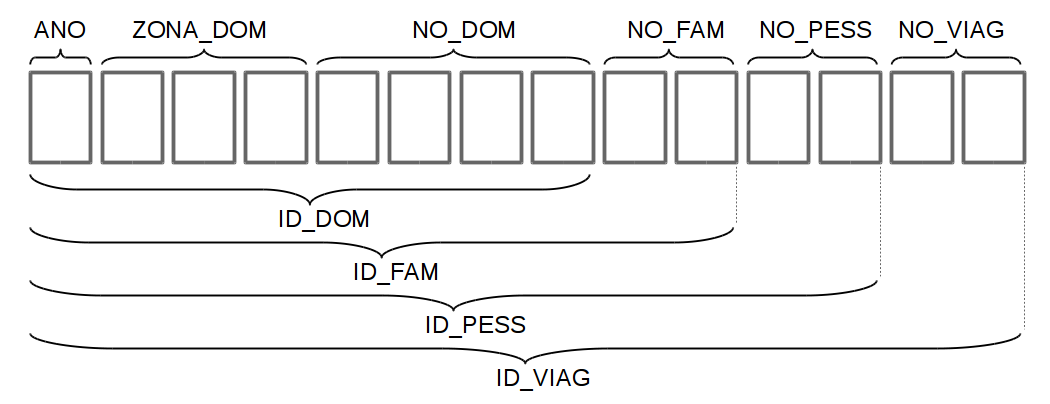
\includegraphics[width=0.75\textwidth]{./imagens/esquema-ID.png}%
    \end{center}%
%    \fonte{Elaboração própria}
\end{figure}%

\item (v) Chamada da função principal: é a parte mais enxuta em termos de código, pois trata apenas da chamada da função principal (\textit{main}), que por sua vez chama as funções gerais.

\end{compactitem} 

\newpage
Vale destacar que, todo esse tratamento de dados visou a compatibilização de categorias entre as diversas Pesquisas OD, que às vezes não continham as mesmas variáveis, ou ainda, não continham as mesmas categorias para uma determinada variável.
Um dos princípios adotados para nova categorização foi agregar para não perder informação. 
Por exemplo, se em 1977 havia as duas categorias ``sem instrução'' e ``primário incompleto'' e, em 1987, havia a categoria ``não alfabetizado/4ª série incompleta'', optou-se por unir as duas categorias de 1977 numa única denominada ``não alfabetizado / fundamental incompleto''. 
Como exemplo, ainda em grau de instrução, do ponto de vista prático houve alterações significativas como: nomenclatura utilizada para os ciclos escolares, formas de ingresso (houve época em que havia um ``vestibulinho'' em algumas escolas para ingressar no ginásio) e quantidade de anos de cada ciclo. 
Além disso, os significados sociais atribuídos à ``mesma variável'' grau de instrução são diferentes ao longo do tempo: ter curso superior no fim da década de 1970 era diferente e muito mais valorado socialmente do que em 2007.
Ou seja, foi feito esforço para minimizar a perda de informações, contudo, algumas limitações são inerentes aos estudos longitudinais e informações são inevitavelmente perdidas, seja pela agregação do dado, seja pela descontinuidade na disponibilização dessa informação.

Foi feito um \textbf{teste de consistência} que consistiu em identificar, para um mesmo indivíduo, que realizou viagem, se a zona de destino da viagem \textit{i} é igual à zona de origem da viagem \textit{i+1}. Inicialmente, foram encontradas 548 observações em 1977\footnote{É preciso considerar que a base de dados 1977 é bastante antiga, rodada originalmente em computadores de grande porte numa época em que não havia computadores pessoais, e que passou por muitas migrações e manipulações até hoje.} que não passaram nesse crivo.  Foi feita análise mais minuciosa desses considerando as variáveis de idade, situação familiar, renda individual, horário de saída e horário de chegada. Observou-se que eram casos de linhas \textit{i} invertidas com as subsequentes, portanto, foram feitas as inversões de linhas e corrigidos 546 registros. Os 2 registros remanescentes foram corrigidos manualmente. Todos os registros de 1987 passaram no teste de consistência. Em 1997, 7 registros não passaram no teste de consistência e, após análise mais cuidadosa, parecia tratar-se de linhas duplicadas, logo, esses 7 registros foram excluídos. Situação semelhante ocorreu com 1 registro de 2007, que também foi excluído.

O Quadro \ref{qua:layout-haydee} apresenta as variáveis do BDU, suas descrições e também tipificação, onde ``Q'' indica tratar-se de variável qualitativa, ``M'', de variável métrica (quantitativa), ``D'', de variável \textit{dummy}, e ``ID'' variável de indexação (natureza texto).

%\clearpage
\newcommand{\layoutTamColA}{0.75cm}
\newcommand{\layoutTamColB}{3.20cm}
\newcommand{\layoutTamColC}{4.20cm}
\newcommand{\layoutTamColD}{0.90cm}
\newcommand{\layoutTamColE}{4.50cm}
\newcommand{\layoutColA}[2]{%
	%2 parâmetros:
	%#1 = número de linhas a serem mescladas
	%#2 = conteúdo da célula
	\multicolumn{1}{|c|}{\multirow{#1}{\layoutTamColA}{\centering#2}}%
}
\newcommand{\layoutColB}[2]{\multicolumn{1}{c|}{\multirow{#1}{\layoutTamColB}{\centering#2}}}
\newcommand{\layoutColC}[2]{\multicolumn{1}{c|}{\multirow{#1}{\layoutTamColC}{\centering#2}}}
\newcommand{\layoutColD}[2]{\multicolumn{1}{c|}{\multirow{#1}{\layoutTamColD}{\centering#2}}}

\begin{quadro}[htb]
    \IBGEtab{
        \renewcommand{\arraystretch}{1.5}
        \ABNTEXfontereduzida
        \caption[Layout]{\label{qua:layout-haydee}\emph{Layout} do Banco de Dados Unificado}
	}{%
        \begin{tabular}{|P{\layoutTamColA}|P{\layoutTamColB}|P{\layoutTamColC}|P{\layoutTamColD}|p{\layoutTamColE}|}
           \hline
   		       \headerCenterCell{Tipo} & 
		       \headerCenterCell{Variável} & 
		       \headerCenterCell{Descrição} & 
		       \headerCenterCell{Qtde. Díg.} & 
		       \headerCenterCell{Códigos, Categorias e Faixas de Valores Válidas}\\ 
		    \hline\hline
		        \layoutColA{4}{Q}&
		        \layoutColB{4}{ANO}&
		        \layoutColC{4}{Ano de referência da Pesquisa OD}&
		        \layoutColD{4}{01}&
		        1 - OD-1977\\
		    	& & & & 2 - OD-1987\\
		    	& & & & 3 - OD-1997\\
		    	& & & & 4 - OD-2007\\
   			\hline
		        \layoutColA{2}{D}&
		        \layoutColB{2}{CD_ENTRE}&
		        \layoutColC{2}{Código de entrevista}&
		        \layoutColD{2}{01}&
		        0 - Completa sem viagem ou incompleta\\
		    	& & & & 1 - Completa com viagem\\
   			\hline
		        \layoutColA{6}{Q}&
		        \layoutColB{6}{DIA_SEM}&
		        \layoutColC{6}{Dia da Semana}&
		        \layoutColD{6}{01}&
		        2 - Segunda-Feira\\
		    	& & & & 3 - Terça-Feira\\
		    	& & & & 4 - Quarta-Feira\\
		    	& & & & 5 - Quinta-Feira\\
		    	& & & & 6 - Sexta-Feira\\
   			\hline
		        {\vfill Q \vfill}&
		        {\vfill UCOD_DOM \vfill}&
		        Unidade de Correspondência de Pesquisas OD para domicílio&
		        {\vfill 02 \vfill}&
				{\vfill 1 a 67\vfill}\\
   			\hline
		        \layoutColA{4}{Q}&
		        \layoutColB{4}{ZONA_DOM}&
		        \layoutColC{4}{Zona do domicílio da OD original}&
		        \layoutColD{4}{03}&
		        1 a 243 em 1977\\
		    	& & & & 1 a 254 em 1987\\
		    	& & & & 1 a 389 em 1997\\
		    	& & & & 1 a 460 em 2007\\
   			\hline
		        \layoutColA{4}{Q}&
		        \layoutColB{4}{SUBZONA_DOM}&
		        \layoutColC{4}{Subzona do domicílio da OD original}&
		        \layoutColD{4}{03}&
		        1 a 633 em 1977\\
		    	& & & & 1 a 9 em 1987\\
		    	& & & & 1 a 9 em 1997\\
		    	& & & & não consta em 2007\\
   			\hline
		\end{tabular}
	}{%
		\fonte{Elaboração própria a partir das OD-1977, OD-1987, OD-1997 e OD-2007}
    }
\end{quadro}

\clearpage
\begin{quadro}[htb]
    \IBGEtab{
        \renewcommand{\arraystretch}{1.5}
        \ABNTEXfontereduzida
        %\caption[Layout]{\label{qua:layout-haydee1}\emph{Layout} do banco de dados integrador das bases OD-1977, OD-1987, OD-1987 e OD2007 - continuação}
	}{%
        \begin{tabular}{|P{\layoutTamColA}|P{\layoutTamColB}|P{\layoutTamColC}|P{\layoutTamColD}|p{\layoutTamColE}|}        
           \hline
   		       \headerCenterCell{Tipo} & 
		       \headerCenterCell{Variável} & 
		       \headerCenterCell{Descrição} & 
		       \headerCenterCell{Qtde. Díg.} & 
		       \headerCenterCell{Códigos, Categorias e Faixas de Valores Válidas}\\ 
		    \hline\hline
		        \layoutColA{4}{Q}&
		        \layoutColB{4}{MUN_DOM}&
		        \layoutColC{4}{Município do domicílio}&
		        \layoutColD{4}{02}&
		        1 a 27 em 1977\\
		    	& & & & 1 a 38 em 1987\\
		    	& & & & 1 a 39 em 1997\\
		    	& & & & 1 a 39 em 2007\\
   			\hline
		        M&
		        CO_DOM_X&
		        \multicolumn{1}{c|}{Coordenada X do domicílio}&
		        12&
				12 dígitos, 2 casas decimais\\
   			\hline
		        M&
		        CO_DOM_Y&
		        \multicolumn{1}{c|}{Coordenada Y do domicílio}&
		        12&
				12 dígitos, 2 casas decimais\\
   			\hline
		        ID&
		        ID_DOM&
		        Identifica o domicílio&
		        08&
		        Composição de ID com ano, zona e domicílio\\
			\hline       
		        \layoutColA{2}{D}&
		        \layoutColB{2}{F_DOM}&
		        \layoutColC{2}{Identifica o primeiro registro do domicílio}&
		        \layoutColD{2}{01}&
		        0 - Demais registros\\
		    	& & & & 1 - Primeiro registro\\
		    \hline
		       	M&
		        FE_DOM&
		        \multicolumn{1}{c|}{Fator de expansão do domicílio}&
		        10&
				10 dígitos, 2 casas decimais\\		        
   			\hline		    	
		        \layoutColA{1}{M}&
		        \layoutColB{1}{NO_DOM}&
		        \layoutColC{1}{Número do domicílio}&
		        \layoutColD{1}{04}&
		        04 dígitos, número inteiro\\
   			\hline
		        \layoutColA{3}{D}&
		        \layoutColB{3}{TIPO_DOM}&
		        \layoutColC{3}{Tipo do domicílio}&
		        \layoutColD{3}{01}&
		        0 - coletivo\\
		        & & & & 1 - particular\\
		    \hline
		       	M&
		        TOT_FAM&
		        \multicolumn{1}{c|}{Total de famílias no domicílio}&
		        02&
				02 dígitos, número inteiro\\			        
   			\hline		    	
		        ID&
		        ID_FAM&
		        Identifica a família&
		        10&
		        Composição de ID com ano, zona, domicílio e família\\
   			\hline		    	
		        \layoutColA{2}{D}&
		        \layoutColB{2}{F_FAM}&
		        \layoutColC{2}{Identifica primeiro registro da família}&
		        \layoutColD{2}{01}&
		        0 - Demais registros\\	
		        & & & & 1 - Primeiro registro\\		        		              
		    \hline
		       	M&
		        FE_FAM&
		        \multicolumn{1}{c|}{Fator de expansão da família}&
		        10&
				10 dígitos, 2 casas decimais\\	
   			\hline		    	
		        \layoutColA{1}{M}&
		        \layoutColB{1}{NO_FAM}&
		        \layoutColC{1}{Número da família}&
		        \layoutColD{1}{02}&
		        02 dígitos, número inteiro\\
   			\hline		    	
		        \layoutColA{4}{Q}&
		        \layoutColB{4}{COND_MORA}&
		        \layoutColC{4}{Condição de moradia}&
		        \layoutColD{4}{01}&
		        1 - alugada\\
		    	& & & & 2 - própria\\
		    	& & & & 3 - outros\\ 	
   			\hline		    	
		        \layoutColA{1}{M}&
		        \layoutColB{1}{QT_AUTO}&
		        \layoutColC{1}{Quantidade de automóveis}&
		        \layoutColD{1}{01}&
		        01 dígito, número inteiro\\
   			\hline		    	
		        \layoutColA{1}{M}&
		        \layoutColB{1}{QT_BICI}&
		        \layoutColC{1}{Quantidade de bicicletas}&
		        \layoutColD{1}{01}&
		        01 dígito, número inteiro\\
   			\hline		    	
		        \layoutColA{1}{M}&
		        \layoutColB{1}{QT_MOTO}&
		        \layoutColC{1}{Quantidade de motocicletas}&
		        \layoutColD{1}{01}&
		        01 dígito, número inteiro\\		        
   			\hline		    	
		        \layoutColA{3}{Q}&
		        \layoutColB{3}{CD_RENFAM}&
		        \layoutColC{3}{Código de renda familiar}&
		        \layoutColD{3}{01}&
		        0 - Renda declarada como zero\\
		        & & & & 1 - Renda declarada maior do que zero\\
		    	& & & & 2 - Renda atribuída\\
   			\hline		    	
		        \layoutColA{1}{M}&
		        \layoutColB{1}{REN_FAM}&
		        \layoutColC{1}{Renda familiar}&
		        \layoutColD{1}{08}&
		        08 dígitos, 2 casas decimais (R\$/mês, ref. out/2007)\\	    	
   			\hline		    		    	
		\end{tabular}
	}{%
		\fonte{Elaboração própria a partir das OD-1977, OD-1987, OD-1997 e OD-2007}
    }
\end{quadro}

\clearpage
\begin{quadro}[htb]
    \IBGEtab{
        \renewcommand{\arraystretch}{1.5}
        \ABNTEXfontereduzida
        %\caption[Layout]{\label{qua:layout-haydee1}\emph{Layout} do banco de dados integrador das bases OD-1977, OD-1987, OD-1987 e OD2007 - continuação}
	}{%
        \begin{tabular}{|P{\layoutTamColA}|P{\layoutTamColB}|P{\layoutTamColC}|P{\layoutTamColD}|p{\layoutTamColE}|}
           \hline
   		       \headerCenterCell{Tipo} & 
		       \headerCenterCell{Variável} & 
		       \headerCenterCell{Descrição} & 
		       \headerCenterCell{Qtde. Díg.} & 
		       \headerCenterCell{Códigos, Categorias e Faixas de Valores Válidas}\\ 
		    \hline\hline
		        ID&
		        ID_PESS&
		        Identifica a pessoa&
		        12&
		        Composição de ID com ano, zona, domicílio, família e pessoa\\	
   			\hline		    	
		        \layoutColA{2}{D}&
		        \layoutColB{2}{F_PESS}&
		        \layoutColC{2}{Identifica o primeiro registro da pessoa}&
		        \layoutColD{2}{01}&
		        0 - Demais registros\\
		        & & & & 1 - Primeiro registro\\	
		    \hline
		       	M&
		        FE_PESS&
		        \multicolumn{1}{c|}{Fator de expansão da pessoa}&
		        10&
				10 dígitos, 2 casas decimais\\	
   			\hline		    	
		        \layoutColA{1}{M}&
		        \layoutColB{1}{NO_PESS}&
		        \layoutColC{1}{Número da pessoa}&
		        \layoutColD{1}{2}&
		        02 dígitos, número inteiro \\
   			\hline			    
		        \layoutColA{6}{Q}&
		        \layoutColB{6}{SIT_FAM}&
		        \layoutColC{6}{Situação familiar}&
		        \layoutColD{6}{01}&
		        1 - Pessoa responsável\\
		        & & & & 2 - Cônjuge/Companheiro(a)\\
		        & & & & 3 - Filho(a)/Enteado(a)\\
		        & & & & 4 - Outro parente / agregado\\
		        & & & & 5 - Empregado residente\\
		        & & & & 6 - Outros\\
		    \hline
		       	M&
		        IDADE&
		        \multicolumn{1}{c|}{Idade}&
		        02&
				02 dígitos, número inteiro\\
		    \hline				
		        \layoutColA{2}{D}&
		        \layoutColB{2}{SEXO}&
		        \layoutColC{2}{Sexo}&
		        \layoutColD{2}{01}&
		        0 - Masculino\\
		        & & & & 1 - Feminino\\
		    \hline				
		        \layoutColA{2}{D}&
		        \layoutColB{2}{ESTUDA}&
		        \layoutColC{2}{A pessoa estuda atualmente?}&
		        \layoutColD{2}{01}&
		        0 - Não\\
		        & & & & 1 - Sim\\
		    \hline				
		        \layoutColA{5}{Q}&
		        \layoutColB{5}{GRAU_INSTR}&
		        \layoutColC{5}{Grau de instrução da pessoa}&
		        \layoutColD{5}{01}&
		        1 - Não alfabetizado / Fundamental incompleto\\
		        & & & & 2 - Fundamental completo / Médio incompleto\\
		        & & & & 3 - Médio completo / Superior incompleto\\
   		        & & & & 4 - Superior completo\\
		    \hline				   		        
		        \layoutColA{8}{Q}&
		        \layoutColB{8}{OCUP}&
		        \layoutColC{8}{Condição de ocupação da pessoa}&
		        \layoutColD{8}{01}&
		        1 - Tem trabalho\\
		        & & & & 2 - Em licença\\
   		        & & & & 3 - Aposentado(a) / Pensionista\\   		        
		        & & & & 4 - Desempregado(a)\\
		        & & & & 5 - Sem ocupação\\
   		        & & & & 6 - Dono(a) de casa\\   		        
		        & & & & 7 - Estudante\\       
			\hline      			
		\end{tabular}
	}{%
		\fonte{Elaboração própria a partir das OD-1977, OD-1987, OD-1997 e OD-2007}
    }
\end{quadro}

\clearpage
\begin{quadro}[htb]
    \IBGEtab{
        \renewcommand{\arraystretch}{1.5}
        \ABNTEXfontereduzida
        %\caption[Layout]{\label{qua:layout-haydee1}\emph{Layout} do banco de dados integrador das bases OD-1977, OD-1987, OD-1987 e OD2007 - continuação}
	}{%
        \begin{tabular}{|P{\layoutTamColA}|P{\layoutTamColB}|P{\layoutTamColC}|P{\layoutTamColD}|p{\layoutTamColE}|}
           \hline
   		       \headerCenterCell{Tipo} & 
		       \headerCenterCell{Variável} & 
		       \headerCenterCell{Descrição} & 
		       \headerCenterCell{Qtde. Díg.} & 
		       \headerCenterCell{Códigos, Categorias e Faixas de Valores Válidas}\\ 
		    \hline\hline
                \layoutColA{10}{Q}&
		        \layoutColB{10}{SETOR_ATIV}&
		        \layoutColC{10}{Setor de atividade (do 1$^o$ trabalho)}&
		        \layoutColD{10}{01}&
		        1 - Agrícola\\
		        & & & & 2 - Construção Civil\\
		        & & & & 3 - Indústria\\
   		        & & & & 4 - Comércio\\   		        
		        & & & & 5 - Administração Pública\\
		        & & & & 6 - Serviços de Transporte\\
   		        & & & & 7 - Outros Serviços\\   		        
		        & & & & 8 - Outros\\
		        & & & & 9 - Não se aplica\\		
   			\hline			        
		        \layoutColA{2}{D}&
		        \layoutColB{2}{CD_RENIND}&
		        \layoutColC{2}{Condição de Renda Individual}&
		        \layoutColD{2}{01}&
		        0 - Não tem renda\\
		        & & & & 1 - Tem renda\\
		    \hline
		       	M&
		        REN_IND&
		        \multicolumn{1}{c|}{Valor da Renda Individual}&
		        08&
				08 dígitos, 2 casas decimais (R\$/mês, ref. out/2007)\\
   			\hline
		        {\vfill Q \vfill}&
		        {\vfill UCOD_ESC \vfill}&
		        Unidade de Correspondência de Pesquisas OD para escola&
		        {\vfill 02 \vfill}&
				{\vfill 1 a 67\vfill}\\
   			\hline
		        \layoutColA{4}{Q}&
		        \layoutColB{4}{ZONA_ESC}&
		        \layoutColC{4}{Zona da escola da OD original}&
		        \layoutColD{4}{03}&
		        1 a 243 em 1977\\
		    	& & & & 1 a 254 em 1987\\
		    	& & & & 1 a 389 em 1997\\
		    	& & & & 1 a 460 em 2007\\
   			\hline
		        \layoutColA{4}{Q}&
		        \layoutColB{4}{SUBZONA_ESC}&
		        \layoutColC{4}{Subzona da escola da OD original}&
		        \layoutColD{4}{03}&
		        1 a 633 em 1977\\
		    	& & & & 1 a 9 em 1987\\
		    	& & & & 1 a 9 em 1997\\
		    	& & & & não consta em 2007\\
   			\hline
		        \layoutColA{4}{Q}&
		        \layoutColB{4}{MUN_ESC}&
		        \layoutColC{4}{Município da escola}&
		        \layoutColD{4}{02}&
		        1 a 27 em 1977\\
		    	& & & & 1 a 39 em 1987\\
		    	& & & & 1 a 39 em 1997\\
		    	& & & & 1 a 39 em 2007\\
   			\hline
		        M&
		        CO_ESC_X&
		        \multicolumn{1}{c|}{Coordenada X da escola}&
		        12&
				12 dígitos, 2 casas decimais\\
   			\hline
		        M&
		        CO_ESC_Y&
		        \multicolumn{1}{c|}{Coordenada Y da escola}&
		        12&
				12 dígitos, 2 casas decimais\\
   			\hline
		        {\vfill Q \vfill}&
		        {\vfill UCOD_TRAB1 \vfill}&
		        Unidade de Correspondência de Pesquisas OD para trabalho 1&
		        {\vfill 02 \vfill}&
				{\vfill 1 a 67\vfill}\\   		    
			\hline      			
		\end{tabular}
	}{%
		\fonte{Elaboração própria a partir das OD-1977, OD-1987, OD-1997 e OD-2007}
    }
\end{quadro}


\clearpage
\begin{quadro}[htb]
    \IBGEtab{
        \renewcommand{\arraystretch}{1.5}
        \ABNTEXfontereduzida
        %\caption[Layout]{\label{qua:layout-haydee1}\emph{Layout} do banco de dados integrador das bases OD-1977, OD-1987, OD-1987 e OD2007 - continuação}
	}{%
        \begin{tabular}{|P{\layoutTamColA}|P{\layoutTamColB}|P{\layoutTamColC}|P{\layoutTamColD}|p{\layoutTamColE}|}
           \hline
   		       \headerCenterCell{Tipo} & 
		       \headerCenterCell{Variável} & 
		       \headerCenterCell{Descrição} & 
		       \headerCenterCell{Qtde. Díg.} & 
		       \headerCenterCell{Códigos, Categorias e Faixas de Valores Válidas}\\ 
		    \hline\hline
		        \layoutColA{4}{Q}&
		        \layoutColB{4}{ZONA_TRAB1}&
		        \layoutColC{4}{Zona do trabalho 1 da OD original}&
		        \layoutColD{4}{03}&
		        1 a 243 em 1977\\
		    	& & & & 1 a 254 em 1987\\
		    	& & & & 1 a 389 em 1997\\
		    	& & & & 1 a 460 em 2007\\
   			\hline
		        \layoutColA{4}{Q}&
		        \layoutColB{4}{SUBZONA_TRAB1}&
		        \layoutColC{4}{Subzona do trabalho 1 da OD original}&
		        \layoutColD{4}{03}&
		        1 a 633 em 1977\\
		    	& & & & 1 a 9 em 1987\\
		    	& & & & 1 a 9 em 1997\\
		    	& & & & não consta em 2007\\
   			\hline
		        \layoutColA{4}{Q}&
		        \layoutColB{4}{MUN_TRAB1}&
		        \layoutColC{4}{Município do trabalho 1}&
		        \layoutColD{4}{02}&
		        1 a 27 em 1977\\
		    	& & & & 1 a 39 em 1987\\
		    	& & & & 1 a 39 em 1997\\
		    	& & & & 1 a 39 em 2007\\	
  			\hline
		        M&
		        CO_TRAB1_X&
		        \multicolumn{1}{c|}{Coordenada X do trabalho 1}&
		        12&
				12 dígitos, 2 casas decimais\\
   			\hline
		        M&
		        CO_TRAB1_Y&
		        \multicolumn{1}{c|}{Coordenada Y do trabalho 1}&
		        12&
				12 dígitos, 2 casas decimais\\	 		    		    
   			\hline   
		        {\vfill Q \vfill}&
		        {\vfill UCOD_TRAB2 \vfill}&
		        Unidade de Correspondência de Pesquisas OD para trabalho 2&
		        {\vfill 02 \vfill}&
				{\vfill 1 a 67\vfill}\\   		    
			\hline  
		        \layoutColA{4}{Q}&
		        \layoutColB{4}{ZONA_TRAB2}&
		        \layoutColC{4}{Zona do trabalho 2 da OD original}&
		        \layoutColD{4}{03}&
		        1 a 243 em 1977\\
		    	& & & & 1 a 254 em 1987\\
		    	& & & & 1 a 389 em 1997\\
		    	& & & & 1 a 460 em 2007\\
   			\hline
		        \layoutColA{4}{Q}&
		        \layoutColB{4}{SUBZONA_TRAB2}&
		        \layoutColC{4}{Subzona do trabalho 2 da OD original}&
		        \layoutColD{4}{03}&
		        1 a 633 em 1977\\
		    	& & & & 1 a 9 em 1987\\
		    	& & & & 1 a 9 em 1997\\
		    	& & & & não consta em 2007\\
   			\hline
		        \layoutColA{4}{Q}&
		        \layoutColB{4}{MUN_TRAB2}&
		        \layoutColC{4}{Município do trabalho 2}&
		        \layoutColD{4}{02}&
		        1 a 27 em 1977\\
		    	& & & & 1 a 39 em 1987\\
		    	& & & & 1 a 39 em 1997\\
		    	& & & & 1 a 39 em 2007\\
   			\hline
		        M&
		        CO_TRAB2_X&
		        \multicolumn{1}{c|}{Coordenada X do trabalho 2}&
		        12&
				12 dígitos, 2 casas decimais\\
   			\hline
		        M&
		        CO_TRAB2_Y&
		        \multicolumn{1}{c|}{Coordenada Y do trabalho 2}&
		        12&
				12 dígitos, 2 casas decimais\\	  
			\hline      				
		\end{tabular}
	}{%
		\fonte{Elaboração própria a partir das OD-1977, OD-1987, OD-1997 e OD-2007}
    }
\end{quadro}

\clearpage
\begin{quadro}[htb]
    \IBGEtab{
        \renewcommand{\arraystretch}{1.5}
        \ABNTEXfontereduzida
        %\caption[Layout]{\label{qua:layout-haydee1}\emph{Layout} do banco de dados integrador das bases OD-1977, OD-1987, OD-1987 e OD2007 - continuação}
	}{%
        \begin{tabular}{|P{\layoutTamColA}|P{\layoutTamColB}|P{\layoutTamColC}|P{\layoutTamColD}|p{\layoutTamColE}|}
           \hline
   		       \headerCenterCell{Tipo} & 
		       \headerCenterCell{Variável} & 
		       \headerCenterCell{Descrição} & 
		       \headerCenterCell{Qtde. Díg.} & 
		       \headerCenterCell{Códigos, Categorias e Faixas de Valores Válidas}\\ 
		    \hline\hline
		        ID&
		        ID_VIAG&
		        Identifica a viagem&
		        14&
		        Composição de ID com ano, zona, domicílio, família, pessoa e viagem\\	
   			\hline		    	
		        \layoutColA{2}{D}&
		        \layoutColB{2}{F_VIAG}&
		        \layoutColC{2}{Identificador de viagem}&
		        \layoutColD{2}{01}&
		        0 - Não fez viagem\\
		        & & & & 1 - Fez viagem\\	
		    \hline
		       	M&
		        FE_VIAG&
		        \multicolumn{1}{c|}{Fator de expansão da viagem}&
		        10&
				10 dígitos, 2 casas decimais\\	
   			\hline		    	
		        \layoutColA{1}{M}&
		        \layoutColB{1}{NO_VIAG}&
		        \layoutColC{1}{Número da viagem}&
		        \layoutColD{1}{02}&
		        02 dígitos, número inteiro \\				
			\hline      							
		       	M&
		        TOT_VIAG&
		        \multicolumn{1}{c|}{Total de viagens da pessoa}&
		        02&
		        02 dígitos, número inteiro \\				
   			\hline   
		        {\vfill Q \vfill}&
		        {\vfill UCOD_ORIG \vfill}&
		        Unidade de Correspondência de Pesquisas OD para origem&
		        {\vfill 02 \vfill}&
				{\vfill 1 a 67\vfill}\\   
			\hline      			
		        \layoutColA{4}{Q}&
		        \layoutColB{4}{ZONA_ORIG}&
		        \layoutColC{4}{Zona de origem da viagem da OD original}&
		        \layoutColD{4}{03}&
		        1 a 243 em 1977\\
		    	& & & & 1 a 254 em 1987\\
		    	& & & & 1 a 389 em 1997\\
		    	& & & & 1 a 460 em 2007\\
   			\hline
		        \layoutColA{4}{Q}&
		        \layoutColB{4}{SUBZONA_ORIG}&
		        \layoutColC{4}{Subzona de origem da viagem da OD original}&
		        \layoutColD{4}{03}&
		        1 a 633 em 1977\\
		    	& & & & 1 a 9 em 1987\\
		    	& & & & 1 a 9 em 1997\\
		    	& & & & não consta em 2007\\
   			\hline
		        \layoutColA{4}{Q}&
		        \layoutColB{4}{MUN_ORIG}&
		        \layoutColC{4}{Município de origem da viagem}&
		        \layoutColD{4}{02}&
		        1 a 27 em 1977\\
		    	& & & & 1 a 39 em 1987\\
		    	& & & & 1 a 39 em 1997\\
		    	& & & & 1 a 39 em 2007\\
   			\hline
		        M&
		        CO_ORIG_X&
		        \multicolumn{1}{c|}{Coordenada X da origem}&
		        12&
				12 dígitos, 2 casas decimais\\
   			\hline
		        M&
		        CO_ORIG_Y&
		        \multicolumn{1}{c|}{Coordenada Y da origem}&
		        12&
				12 dígitos, 2 casas decimais\\			    
   			\hline		    
		        {\vfill Q \vfill}&
		        {\vfill UCOD_DEST \vfill}&
		        Unidade de Correspondência de Pesquisas OD para destino&
		        {\vfill 02 \vfill}&
				{\vfill 1 a 67\vfill}\\   
			\hline    
		        \layoutColA{4}{Q}&
		        \layoutColB{4}{ZONA_DEST}&
		        \layoutColC{4}{Zona de destino da viagem da OD original}&
		        \layoutColD{4}{03}&
		        1 a 243 em 1977\\
		    	& & & & 1 a 254 em 1987\\
		    	& & & & 1 a 389 em 1997\\
		    	& & & & 1 a 460 em 2007\\
   			\hline
		        \layoutColA{4}{Q}&
		        \layoutColB{4}{SUBZONA_DEST}&
		        \layoutColC{4}{Subzona de destino da viagem da OD original}&
		        \layoutColD{4}{03}&
		        1 a 633 em 1977\\
		    	& & & & 1 a 9 em 1987\\
		    	& & & & 1 a 9 em 1997\\
		    	& & & & não consta em 2007\\
   			\hline	  					
		\end{tabular}
	}{%
		\fonte{Elaboração própria a partir das OD-1977, OD-1987, OD-1997 e OD-2007}
    }
\end{quadro}

\clearpage
\begin{quadro}[htb]
    \IBGEtab{
        \renewcommand{\arraystretch}{1.5}
        \ABNTEXfontereduzida
        %\caption[Layout]{\label{qua:layout-haydee1}\emph{Layout} do banco de dados integrador das bases OD-1977, OD-1987, OD-1987 e OD2007 - continuação}
	}{%
        \begin{tabular}{|P{\layoutTamColA}|P{\layoutTamColB}|P{\layoutTamColC}|P{\layoutTamColD}|p{\layoutTamColE}|}
           \hline
   		       \headerCenterCell{Tipo} & 
		       \headerCenterCell{Variável} & 
		       \headerCenterCell{Descrição} & 
		       \headerCenterCell{Qtde. Díg.} & 
		       \headerCenterCell{Códigos, Categorias e Faixas de Valores Válidas}\\ 
		    \hline\hline
		        \layoutColA{4}{Q}&
		        \layoutColB{4}{MUN_DEST}&
		        \layoutColC{4}{Município de destino da viagem}&
		        \layoutColD{4}{02}&
		        1 a 27 em 1977\\
		    	& & & & 1 a 39 em 1987\\
		    	& & & & 1 a 39 em 1997\\
		    	& & & & 1 a 39 em 2007\\
   			\hline
		        M&
		        CO_DEST_X&
		        \multicolumn{1}{c|}{Coordenada X do destino}&
		        12&
				12 dígitos, 2 casas decimais\\
   			\hline
		        M&
		        CO_DEST_Y&
		        \multicolumn{1}{c|}{Coordenada Y do destino}&
		        12&
				12 dígitos, 2 casas decimais\\	
   			\hline
		        M&
		        DIST_VIAG&
		        \multicolumn{1}{c|}{Distância da viagem (m)}&
		        08&
				08 dígitos, 2 casas decimais\\		
   			\hline				
		        \layoutColA{2}{D}&
		        \layoutColB{2}{SERV_PAS_ORIG}&
		        \layoutColC{2}{Serve passageiro na origem?}&
		        \layoutColD{2}{01}&
		        0 - Não\\
		        & & & & 1 - Sim\\					
   			\hline				
		        \layoutColA{2}{D}&
		        \layoutColB{2}{SERV_PAS_DEST}&
		        \layoutColC{2}{Serve passageiro no destino?}&
		        \layoutColD{2}{01}&
		        0 - Não\\
		        & & & & 1 - Sim\\							
   			\hline
		        \layoutColA{9}{Q}&
		        \layoutColB{9}{MOTIVO_ORIG}&
		        \layoutColC{9}{Motivo na origem}&
		        \layoutColD{9}{01}&
		        1 - Trabalho (indústria)\\
		        & & & & 2 - Trabalho (comércio)\\
		        & & & & 3 - Trabalho (serviços)\\
   		        & & & & 4 - Educação\\   		        
		        & & & & 5 - Compras\\
		        & & & & 6 - Saúde\\
   		        & & & & 7 - Lazer\\   		        
		        & & & & 8 - Residência\\
		        & & & & 9 - Outros\\		        
   			\hline			    
		        Q&
		        MOTIVO_DEST&
		        \multicolumn{1}{c|}{Motivo no destino}&
		        02&
				idem Motivo na origem\\			    
   			\hline
		        \layoutColA{12}{Q}&
		        \layoutColB{12}{MODO1}&
		        \layoutColC{12}{Modo 1}&
		        \layoutColD{12}{2}&
		        1 - Ônibus de linha\\
		        & & & & 2 - Ônibus escolar / empresa\\
		        & & & & 3 - Dirigindo automóvel\\
   		        & & & & 4 - Passageiro de automóvel\\   		        
		        & & & & 5 - Táxi\\
		        & & & & 6 - Lotação / van\\
   		        & & & & 7 - Metrô\\   		        
		        & & & & 8 - Trem\\
		        & & & & 9 - Motocicleta\\				
		        & & & & 10 - Bicicleta\\						        
		        & & & & 11 - A pé\\						        
		        & & & & 12 - Outros\\	
   			\hline
		\end{tabular}
	}{%
		\fonte{Elaboração própria a partir das OD-1977, OD-1987, OD-1997 e OD-2007}
    }
\end{quadro}

\clearpage
\begin{quadro}[htb]
    \IBGEtab{
        \renewcommand{\arraystretch}{1.5}
        \ABNTEXfontereduzida
        %\caption[Layout]{\label{qua:layout-haydee1}\emph{Layout} do banco de dados integrador das bases OD-1977, OD-1987, OD-1987 e OD2007 - continuação}
	}{%
        \begin{tabular}{|P{\layoutTamColA}|P{\layoutTamColB}|P{\layoutTamColC}|P{\layoutTamColD}|p{\layoutTamColE}|}
           \hline
   		       \headerCenterCell{Tipo} & 
		       \headerCenterCell{Variável} & 
		       \headerCenterCell{Descrição} & 
		       \headerCenterCell{Qtde. Díg.} & 
		       \headerCenterCell{Códigos, Categorias e Faixas de Valores Válidas}\\  
		    \hline\hline  			  
		        Q&
		        MODO2&
		        \multicolumn{1}{c|}{Modo 2}&
		        02&
				idem Modo 1\\	
   			\hline	
		        Q&
		        MODO3&
		        \multicolumn{1}{c|}{Modo 3}&
		        02&
				idem Modo 1\\	
   			\hline	
		        Q&
		        MODO4&
		        \multicolumn{1}{c|}{Modo 4}&
		        02&
				idem Modo 1\\	
   			\hline	
		        Q&
		        MODO_PRIN&
		        \multicolumn{1}{c|}{Modo Principal}&
		        02&
				idem Modo 1\\	
   			\hline	
		        \layoutColA{3}{Q}&
		        \layoutColB{3}{TIPO_VIAG}&
		        \layoutColC{3}{Tipo de viagem}&
		        \layoutColD{3}{01}&
		        1 - Coletivo\\
		        & & & & 2 - Individual\\
		        & & & & 3 - A pé\\
   			\hline	
		        M&
		        H_SAIDA&
		        \multicolumn{1}{c|}{Hora de saída}&
		        02&
				Hora de saída\\	
   			\hline	
		        M&
		        MIN_SAIDA&
		        \multicolumn{1}{c|}{Minuto de saída}&
		        02&
				Minutos de saída\\
   			\hline	
		        M&
		        ANDA_ORIG&
		        \multicolumn{1}{c|}{Tempo andando na origem}&
		        02&
				Tempo andando na origem (minutos)\\	
   			\hline	
		        M&
		        H_CHEG&
		        \multicolumn{1}{c|}{Hora de chegada}&
		        02&
				Hora de chegada\\	
   			\hline	
		        M&
		        MIN_CHEG&
		        \multicolumn{1}{c|}{Minuto de chegada}&
		        02&
				Minutos de chegada\\
   			\hline	
		        M&
		        ANDA_DEST&
		        \multicolumn{1}{c|}{Tempo andando no destino}&
		        02&
				Tempo andando no destino (minutos)\\	
   			\hline	
		        M&
		        DURACAO&
		        \multicolumn{1}{c|}{Duração da viagem}&
		        02&
				Duração da viagem (minutos)\\	
   			\hline		
		        \layoutColA{3}{Q}&
		        \layoutColB{3}{TIPO_EST_AUTO}&
		        \layoutColC{3}{Tipo de estacionamento}&
		        \layoutColD{3}{01}&
		        0 - não estacionou\\
 		        & & & & 1 - estacionou em local privado (particular avulso ou mensal, próprio ou patrocinado)\\
		        & & & & 2 - estacioanou em local público (na rua)\\				
   			\hline
		        M&
		        VALOR_EST&
		        \multicolumn{1}{c|}{Valor do estacionamento}&
		        02&
				06 dígitos, 2 casas decimais (R\$/mês, ref. out/2007)\\	
   			\hline											   					
		\end{tabular}
	}{%
		\fonte{Elaboração própria a partir das OD-1977, OD-1987, OD-1997 e OD-2007}
    }
\end{quadro}

\section{Critérios de Validação}\label{sec:bd-validacao}

Algumas variáveis (colunas) inicialmente não identificadas como de interesse para este trabalho foram descartadas dos bancos originais.
Dado o interesse em investigar o comportamento de homens e mulheres nos deslocamentos diários, o critério utilizado para a exclusão de observações (linhas) foi a variável ``SEXO'' ser igual a 0 na base de dados.
Assim, após a preparação da base e da execução de testes de consistência, foram excluídas 1561 linhas - todas pertencentes a 1977 e cujo fator de expansão de viagens também era igual a 0. O impacto na quantidade de domicílios, pessoas e viagens (registros) está expresso na Tabela \ref{tab:qtde-viagens}. 

\begin{table}[htb]
    \IBGEtab{%\renewcommand{\arraystretch}{1.5}%%\ABNTEXfontereduzida%
	    \renewcommand{\arraystretch}{1.5}
        \caption{Quantidade de viagens e de domicílios, por ano, antes e depois da preparação do BDU}
		\label{tab:qtde-viagens}
    }{%
    \begin{tabular}{ccccccc}
		\toprule
		\multirow{2}{*}{\textbf{Ano}} & \multicolumn{2}{c}{\textbf{Número de Domicílios}} & \multicolumn{2}{c}{\textbf{Número de Pessoas}} & \multicolumn{2}{c}{\textbf{Número de Viagens}} \\ \cline{2-7}
		& \textbf{Antes} & \textbf{Depois} & \textbf{Antes} & \textbf{Depois} & \textbf{Antes} & \textbf{Depois} \\ \midrule \midrule
				1977 & 26.132 & 24.613 & 108.069 & 108.028 & 230.606 & 229.045\\ \hline
				1987 & 26.070 & 26.070 & 110.813 & 110.813 & 223.926 & 223.926\\ \hline
				1997 & 23.841 & 23.841 & 98.780 & 98.780 & 199.647 & 199.647\\ \hline
		        2007 & 29.957 & 29.957 & 91.405 & 91.405 & 196.698 & 196.698\\ \hline  
		        Total & 106.000 & 104.481 & 409.067 & 409.025 & 850.877 & 849.316\\ \bottomrule	
	\end{tabular}
    }{%
		\fonte{Compilação a partir de \cite{OD77,OD87,OD97,OD07}}
	}
\end{table}

Os critérios para a adoção de ``NA'' foram os seguintes:

\begin{compactitem}[]
\item (i) Quando em um ano específico não havia informação levantada para uma determinada variável.
\item (ii) Quando, mesmo essa variável tendo sido levantada, não houve preenchimento ou resposta.
\item (iii) Quando uma determinada informação não existe pelo do fato de que não foi feita viagem.
\end{compactitem}


\section{Formulação de Novas Variáveis}\label{sec:bd-novas-var}

Foram criadas variáveis de interesse, relativas a viagens, pessoas ou famílias, para gerar informações necessárias para subsidiar as análises subsequentes.
Além dessas, também foram criadas 4 \textit{dummies} de ano (ANO_77, ANO_87, ANO_97 e ANO_97) para que fosse possível, nas regressões, tentar captar o efeito do tempo.

\subsection{Variáveis relativas às viagens}\label{subsec:novas-var-viag}

\begin{compactitem}

\item \textbf{Faixa horária e \textit{dummies} de período}: A variável FAIXA_HORARIA foi criada para classificar as viagens em faixas horárias, considerando o horário de término da viagem obtido a partir das variáveis H_CHEG (hora de chegada) e MIN_CHEG (minuto de chegada).
Isso porque o horário de chegada corresponde ao horário de início da atividade que motivou a viagem, e são as atividades que, de fato, interessam e motivam o comportamento humano. 
Foram adotadas sete categorias para a divisão dos períodos do dia, derivados do estudo de \citeauthoronline{VESPUCCI2003} (\citeyear{VESPUCCI2003}).
Para cada faixa horária, foi gerada uma \textit{dummy} de período correspondente. Tal divisão, também adotada por \citeauthoronline{GERMANI2005} (\citeyear{GERMANI2005}), foi a que melhor refletiu as concentrações de atividades e é a seguinte:
    \begin{compactitem}[]
    \item 0 -> não fez viagem 
    \item 1 -> madrugada (entre 0h01 e 5h00), originou a \textit{dummy} VIAG_PER_MADRUG
    \item 2 -> começo da manhã (entre 5h01 e 9h00), originou a \textit{dummy} VIAG_PER_COM_MAN
    \item 3 -> manhã (entre 9h01 e 12h), originou a \textit{dummy} VIAG_PER_MANHA
    \item 4 -> meio-dia tarde (entre 12h01 e 14h), originou a \textit{dummy} VIAG_PER_MEIODIA
    \item 5 -> tarde (entre 14h01 e 17h), originou a \textit{dummy} VIAG_PER_TARDE
    \item 6 -> começo da noite (17h01 e 22h), originou a \textit{dummy} VIAG_PER_COM_NOI
    \item 7 -> noite (22h01 e 0h), originou a \textit{dummy} VIAG_PER_NOITE
    \end{compactitem}\

\item \textbf{Contagem da utilização dos modos}: Como cada viagem pode comportar a utilização de até 4 modos\footnote{As pesquisas OD-77 e OD-87 previam campo para até 3 modos, já as pesquisas OD-97 e OD-07 previam a utilização de até 4 modos por viagem.} é feita a contagem de quantas vezes um determinado modo foi utilizado em uma viagem.
Quem não fez viagem terá toda as variáveis listadas a seguir definidas como iguais a 0. A consolidação da quantidade de modos diferentes utilizados na viagem é sumarizado na variável VIAG_NO_MODOS. 

    \begin{compactitem}[]
    \item VIAG_MODO_ONIBUS -> viagens feitas por ônibus de linha (municipal ou intermunicipal), ônibus escolar, ônibus de empresa, lotação e van
    \item VIAG_MODO_DIRIG -> viagens feitas por automóvel com a pessoa dirigindo
    \item VIAG_MODO_PASS -> viagens feitas por automóvel com a pessoa como passageiro, incluindo as viagens de táxi
    \item VIAG_MODO_TREM -> viagens feitas por metrô ou trem
    \item VIAG_MODO_MOTO -> viagens feitas por motocicleta
    \item VIAG_MODO_BICI -> viagens feitas por bicicleta
    \item VIAG_MODO_APE -> viagens feitas a pé
    \item VIAG_MODO_OUTROS -> viagens não contempladas pelas categorias anteriores
    \item VIAG_NO_MODOS -> quantos modos diferentes foram utilizados, por viagem, de acordo com estas categorias
    \end{compactitem}\

\item \textbf{\textit{Dummies} dos motivos de viagem}: Cada viagem só tem um motivo na origem e um motivo no destino.
Foram considerados os motivos do destino (que relacionam-se com a atividade fim daquele deslocamento) e criados seis marcadores, conforme pode ser observado a seguir. 
\citeauthoronline{VESPUCCI2003}\footnote{Fez estudos sobre a sequência diária de atividades e cadeias de viagens a partir das pesquisas OD-87 e OD-97.} (\citeyear{VESPUCCI2003}) e \citeauthoronline{GERMANI2005}\footnote{Fez estudos sobre comportamento de demanda usando método de alinhamento de sequências multidimensionais a partir da pesquisa OD-97.} (\citeyear{GERMANI2005}) agregam as viagens denominadas de manutenção  (como compras e saúde) com as de lazer e outros, além de desagregar as viagens de motivo residência em temporária e final. 
\citeauthoronline{DALMASO2009}\footnote{Fez estudos sobre a identificação e caracterização de grupos de indivíduos segundo padrões de sequências de atividades multidimensionais a partir da pesquisa OD-97.} (\citeyear{DALMASO2009}) verificou que os resultados desta categorização eram muito parecidos.
Além disso, este autor constatou que havia grandes diferenças nos resultados mantendo o motivo manutenção único ou desmembrando-o em compras/saúde e lazer/outros.
Por fim, ele considerou o motivo ``servir passageiro'', que significa que a pessoa ao fazer uma viagem para acompanhar alguém (à escola, ao médico, etc.) não faz essa viagem por um motivo seu, mas acompanhando o motivo da outra pessoa, a quem ``serve''.
Optou-se por seguir a divisão de categorias de motivos de \citeauthoronline{DALMASO2009} (unificação de motivo residência, separação do motivo manutenção e explicitação do motivo servir passageiro) porque a revisão de literatura indica que as mulheres são as principais cuidadoras do núcleo familiar, assim, espera-se que apresentem maior frequência nos motivos ``servir passageiro'' e, talvez, no ``manutenção/compras'' do que os homens.
    \begin{compactitem}[]
    \item VIAG_MOTIVO_SERV_PAS -> \textit{dummy} da viagem motivo servir passageiro
    \item VIAG_MOTIVO_TRAB -> \textit{dummy} da viagem motivo trabalho
    \item VIAG_MOTIVO_EDUC -> \textit{dummy} da viagem motivo educação
    \item VIAG_MOTIVO_RES -> \textit{dummy} da viagem motivo residência
    \item VIAG_MOTIVO_MANUT_COMPRAS -> \textit{dummy} da viagem motivo manutenção da casa (compras) ou da família (saúde)
    \item VIAG_MOTIVO_LAZER_OUTROS -> \textit{dummy} da viagem motivo destino lazer ou outros
    \end{compactitem}\

\item \textbf{\textit{Dummies} de viagens inter-zonas}: Foi criado um marcador que indicasse quando uma viagem teve sua zona de destino distinta da sua zona de origem. Não se busca mensurar distância ou tempo, mas a eventual superação de barreiras urbanas. Uma viagem intrazonal pode ser mais longa (em tempo e distância) que uma viagem interzonal, e mesmo assim ser preferível. Em São Paulo, por exemplo, a distância de uma margem a outra da Marginal Pinheiros, ou mesmo o tempo levado apenas para atravessar um de suas pontes, não representam valores muito grandes. Porém, é comum que os munícipes optem por fazer suas atividades (e deslocamentos) apenas de um lado do rio, pois este constitui-se uma barreira urbana, um ponto de impedância no sistema de deslocamentos. O desenho do zoneamento das pesquisas OD não foi formulado com a intenção de evidenciar as barreiras urbanas, mas mesmo assim, as reflete.
% Pegar mapas e marcar as barreiras urbanas sobre o zoneamento
% Por referências sobre barreiras urbanas (Andreina, Castells)

\end{compactitem}

\subsection{Variáveis relativas às pessoas}\label{subsec:novas-var-pess}

\begin{compactitem}

\item \textbf{Faixa etária e \textit{dummies} de faixa etária}: A partir da variável IDADE, foi criada a variável FAIXA_ETARIA, seguindo os critérios adotados pelo IBGE, resultando em 21 faixas etárias, conforme pode ser observado a seguir. Para cada faixa etária, foi gerada uma \textit{dummy} correspondente.
    \begin{compactitem}[]
    \item 0 -> 0 a 4 anos, originou a \textit{dummy} FX_ET_0
	\item 1 -> 5 a 9 anos, originou a \textit{dummy} FX_ET_1
	\item 2 -> 10 a 14 anos, originou a \textit{dummy} FX_ET_2
	\item 3 -> 15 a 19 anos, originou a \textit{dummy} FX_ET_3
	\item 4 -> 20 a 24 anos, originou a \textit{dummy} FX_ET_4
	\item 5 -> 25 a 29 anos, originou a \textit{dummy} FX_ET_5
	\item 6 -> 30 a 34 anos, originou a \textit{dummy} FX_ET_6
	\item 7 -> 35 a 39 anos, originou a \textit{dummy} FX_ET_7
	\item 8 -> 40 a 44 anos, originou a \textit{dummy} FX_ET_8
	\item 9 -> 45 a 49 anos, originou a \textit{dummy} FX_ET_9
	\item 10 -> 50 a 54 anos, originou a \textit{dummy} FX_ET_10
	\item 11 -> 55 a 59 anos, originou a \textit{dummy} FX_ET_11
	\item 12 -> 60 a 64 anos, originou a \textit{dummy} FX_ET_12
	\item 13 -> 65 a 69 anos, originou a \textit{dummy} FX_ET_13
	\item 14 -> 70 a 74 anos, originou a \textit{dummy} FX_ET_14
	\item 15 -> 75 a 79 anos, originou a \textit{dummy} FX_ET_15
	\item 16 -> 80 a 84 anos, originou a \textit{dummy} FX_ET_16
	\item 17 -> 85 a 89 anos, originou a \textit{dummy} FX_ET_17
	\item 18 -> 90 a 94 anos, originou a \textit{dummy} FX_ET_18
	\item 19 -> 95 a 99 anos, originou a \textit{dummy} FX_ET_19
	\item 20 -> mais de 100 anos, originou a \textit{dummy} FX_ET_20
    \end{compactitem}\

\item \textbf{Faixa de renda individual}: Os valores de renda individual foram levados para out/2007 e classificados em sete categorias explicitadas a seguir, conforme a quantidade de salários mínimos (SM)\footnote{O valor de um salário mínimo era R\$380,00 em 2007 segundo a Lei do salário mínimo vigente e disponível em \url{ https://www.planalto.gov.br/ccivil_03/_Ato2007-2010/2007/Lei/L11498.htm} Acesso em 30 de setembro de 2015.}.
    \begin{compactitem}[]
    \item 0 -> sem renda
    \item até R\$380 (exclusive) -> até 1 SM
    \item de R\$380 (inclusive) até R\$760 (exclusive) -> de 1 a 2 SM
    \item de R\$760 (inclusive) até R\$1140 (exclusive) -> de 2 a 3 SM
    \item de R\$1140 (inclusive) até R\$1900 (exclusive) -> de 3 a 5 SM
    \item de R\$1900 (inclusive) até R\$3800 (exclusive) -> de 5 a 10 SM
    \item de R\$3800 (inclusive) até R\$5700 (exclusive) -> de 10 a 15 SM 
    \item mais de R\$5700 (inclusive) -> mais de 15 SM        
    \end{compactitem}\

\newpage
\item \textbf{Contagem da utilização dos modos}: Baseadas nas variáveis de contagem de modo foi calculada a variável PESS_NO_MODOS, que sintetiza a quantidade de modos diferentes que a pessoa utilizou ao longo do dia, segundo a Equação \eqref{eq:pess-modo}, onde K é o número de categorias dos modos.

\begin{equation}\label{eq:pess-modo}
\begin{split}
PESS\_NO\_MODOS=\displaystyle\sum_{k=1}^{K}USO\_MODO_{k},\ \text{onde}:\\
\begin{cases}
        USO\_MODO_{k}=0 & \ \text{se}\  VIAG\_MODO_{k}=0\\
        USO\_MODO_{k}=1 & \ \text{se}\  VIAG\_MODO_{k} \neq 0\\
\end{cases}
\end{split}
\end{equation}

\item \textbf{Contagem dos motivos de viagem}: Baseadas nas \textit{dummies} dos motivos das viagens, foram feitos agrupamentos por pessoas, e somadas a quantidade de vezes que um determinado motivo foi declarado para cada pessoa - ver Equação \eqref{eq:pess-motivo}, onde n é o número de viagens da pessoa.
A variável PESS_NO_MOTIVOS sintetiza a quantidade de motivos diferentes que levou a pessoa a se deslocar ao longo do dia.

\begin{equation}\label{eq:pess-motivo}
PESS\_NO\_MOTIVOS=\displaystyle\sum_{i=1}^{n}VIAG\_MOTIVO_{i}
\end{equation}

\item \textbf{Distância total}: A informação das distâncias percorridas por viagem já está armazenada na variável DIST_VIAG do BDU. A variável PESS_DIST_TOT sumariza essa informação para a pessoa, conforme Equação \eqref{eq:pess-dist-tot}, onde n é o número de viagens da pessoa.

\begin{equation}\label{eq:pess-dist-tot}
PESS\_DIST\_TOT=\displaystyle\sum_{i=1}^{n}DIST\_VIAG_{i}
\end{equation}

\item \textbf{Distância média}: A distância média percorrida pela pessoa é a distância total da pessoa dividida pelo seu número total de viagens - ver Equação \eqref{eq:pess-dist-med}, onde n é o número de viagens da pessoa.

\begin{equation}\label{eq:pess-dist-med}
PESS\_DIST\_MED=\frac{\displaystyle\sum_{i=1}^{n}DIST\_VIAG_{i}}{TOT\_VIAG}
\end{equation}

\item \textbf{Duração total}: A informação das distâncias percorridas por viagem já está armazenada na variável DURACAO do BDU. A variável PESS_DURACAO_TOT sumariza essa informação para a pessoa, conforme Equação \eqref{eq:pess-dur-tot}, onde n é o número de viagens da pessoa.

\begin{equation}\label{eq:pess-dur-tot}
PESS\_DURACAO\_TOT=\displaystyle\sum_{i=1}^{n}DURACAO_{i}
\end{equation}

\item \textbf{Duração média}: A duração média percorrida pela pessoa é a duração total da pessoa dividida pelo seu número total de viagens - ver Equação \eqref{eq:pess-dur-med}, onde n é o número de viagens da pessoa.

\begin{equation}\label{eq:pess-dur-med}
PESS\_DURACAO\_MED=\frac{\displaystyle\sum_{i=1}^{n}DURACAO_{i}}{TOT\_VIAG}
\end{equation}\\

\end{compactitem}

\subsection{Variáveis relativas às famílias}\label{subsec:novas-var-fam}

\begin{compactitem}

\item \textbf{Tamanho da família}: O tamanho da família (variável TOT_PESS) é determinado pelo máximo número da pessoa (NO_PESS) de uma determinada família.\\

\item \textbf{Faixa de renda familiar}: A partir da variável renda familiar, em valores de outubro de 2007, foi criada a variável FAIXA_REN_FAM, que contém a faixa de renda familiar segundo o critério de classificação do IBGE para classes econômicas
\footnote{Definição de Classe Econômica – Fonte: \url{http://www.sae.gov.br/wp-content/uploads/ebook_ClasseMedia1.pdf} Acesso em 30 de setembro de 2015.} (A, B, C, D e E) – ver categorias abaixo. Portanto, as faixas de renda familiar foram construídas a partir da quantidade de salários mínimos, sendo o valor de um salário mínimo R\$380,00 em 2007
\footnote{Lei do salário mínimo de 2007: \url{ https://www.planalto.gov.br/ccivil_03/_Ato2007-2010/2007/Lei/L11498.htm} Acesso em 30 de setembro de 2015.}.
    \begin{compactitem}[]
    \item 0 -> sem renda
    \item até R\$760 (exclusive) -> Classe E
    \item de R\$760 (inclusive) até R\$1520 (exclusive) -> Classe D
    \item de R\$1520 (inclusive) até R\$3800 (exclusive) -> Classe C
    \item de R\$3800 (inclusive) até R\$7600 (exclusive) -> Classe B
    \item mais de R\$7600 (inclusive) -> Classe A
    \end{compactitem}\

\item \textbf{Número total de viagens da família}: A variável FAM_VIAG_TOT é calculada como a soma do número de viagens de cada pessoa da família - ver Equação \eqref{eq:fam-viag-tot}, onde p é o número de pessoas da família.

\begin{equation}\label{eq:fam-viag-tot}
FAM\_VIAG\_TOT=\displaystyle\sum_{j=1}^{p}TOT\_VIAG_{j}
\end{equation}

\newpage
\item \textbf{Distância total}:  A informação das distâncias percorridas por viagem já está armazenada na variável DIST_VIAG do BDU. A variável FAM_DIST_TOT sumariza essa informação para a família, conforme Equação \eqref{eq:fam-dist-tot}, onde p é o número de pessoas da família.

\begin{equation}\label{eq:fam-dist-tot}
FAM\_DIST\_TOT=\displaystyle\sum_{j=1}^{p}PESS\_DIST\_TOT_{j}
\end{equation}

\item \textbf{Distância média}: A distância média de uma viagem da famílias, calculada como a soma das distâncias das pessoas dividida pelo seu total de viagens da família - ver Equação \eqref{eq:fam-dist-med}, onde p é o número de pessoas da família.

\begin{equation}\label{eq:fam-dist-med}
FAM\_DIST\_MED=\frac{\displaystyle\sum_{j=1}^{p}PESS\_DIST\_TOT_{j}}{FAM\_VIAG\_TOT}
\end{equation}\\

\item \textbf{Duração total}: A duração total das viagens da família são armazenadas na variável FAM_DURACAO_TOT, que sumariza essa informação para a família, conforme Equação \eqref{eq:fam-dur-tot}, onde p é o número de pessoas da família.

\begin{equation}\label{eq:fam-dur-tot}
FAM\_DURACAO\_TOT=\displaystyle\sum_{j=1}^{p}PESS\_DURACAO\_TOT_{j}
\end{equation}

\item \textbf{Duração média}: A duração média de uma viagem da família é armazenada na variável FAM_DURACAO_MED, que soma a duração total das pessoas da família e divide pelo seu número total de viagens da família - ver Equação \eqref{eq:fam-dur-med}, onde p é o número de pessoas da família.

\begin{equation}\label{eq:fam-dur-med}
FAM\_DURACAO\_MED=\frac{\displaystyle\sum_{j=1}^{p}PESS\_DURACAO\_TOT_{j}}{FAM\_VIAG\_TOT}
\end{equation}\\

\item \textbf{Presença de automóveis na família}: Foi gerada uma \textit{dummy} (PRESENCA_AUTO) para indicar a presença de automóvel na família.
Segundo \apudonline{STRAMBI2001}{PEIXOTO2002} a motorização é um fator de grande influência sobre o padrão de mobilidade. 
\citeauthoronline{PEIXOTO2002}\ (\citeyear{PEIXOTO2002}), ao estudar a evolução temporal da mobilidade na Região Metropolitana de Porto Alegre, entre 1986 e 1997, detectou ser a posse de veículos uma característica importante para segmentação de grupos de comportamento semelhantes.
Geralmente, a utilização do automóvel é decidida dentro de uma determinada dinâmica familiar.
No contexto familiar surgem questões como: em não existindo um automóvel para cada pessoa habilitada, quem tem a prioridade no uso? Quem trabalha mais longe de casa? Quem tem uma rotina mais complexa? Quem leva os filhos na escola? Quem é autônomo?\\

\item \textbf{Presença de crianças na família}: Como um indicativo do estágio no ciclo de vida familiar \cite{ORTUZAR1994}, foram geradas \textit{dummies} para indicar, na família, a presença de crianças/adolescentes de quatro faixas etárias, a saber: 

    \begin{compactitem}[]
    \item PRESENCA_FILH_ate4 -> indica se a família conta com crianças até 4 anos
    \item PRESENCA_FILH_5a9 -> indica se a família conta com crianças entre 5 e 9 anos
    \item PRESENCA_FILH_10a14 -> indica se a família conta com crianças entre 10 e 14 anos
    \item PRESENCA_FILH_15a19 -> indica se a família conta com adolescentes entre 15 e 19 anos
    \end{compactitem}\

\item \textbf{Presença de idosos na família}: A presença de idoso na família, também é um indicativo de estágio no ciclo de vida familiar \cite{ORTUZAR1994}, tanto mais expressivo quanto mais a população envelhece. 
\citeauthoronline{OLIVEIRA2014}\ (\citeyear{OLIVEIRA2014}) ao estudar a correlação e efeitos das composições familiares na
mobilidade do idoso, considerando aspectos econômicos e sociais, constatou que o tamanho da família afeta negativamente a mobilidade dos idosos e que quanto maior o número de idosos na mesma família, maior sua mobilidade. 
\citeauthoronline{VASCONCELLOS2001}\ (\citeyear{VASCONCELLOS2001}) aponta que aspectos econômicos e sociais influenciam os padrões de mobilidade das pessoas e destaca, dentre os sociais, a família como um dos fatores importantes na tomada de decisões em relação aos deslocamentos e arranjos das atividades diárias. Como o próprio conceito de quem é idoso vem mudando com o tempo, e este trabalho observa quatro \textit{cross sections} e três décadas, decidiu-se por destacar a presença de idosos em duas faixas etárias:

    \begin{compactitem}[]
    \item PRESENCA_IDOSO_60_70 -> indica se a família conta com pessoa idosa entre 60 e 70 anos
    \item PRESENCA_IDOSO_70 -> indica se a família conta com pessoa idosa com mais de 70 anos
    \end{compactitem}

\end{compactitem}
% ----------------------------------------------------------
% Capitulo das Analises Realizadas
% ---
% ---
% Capitulo Análises
% ---
\chapter{Análises Realizadas}\label{chap:analises}

\section{Estatísticas Descritivas}\label{sec:bd-estat-descr}

A seguir serão apresentadas algumas estatísticas descritivas das variáveis, bem como outras observações julgadas pertinentes.

A variável \textbf{ANO}, de natureza qualitativa, não possui ``NA'' e conta com quatro valores únicos, cujas frequências absolutas são apresentadas na Tabela \ref{tab:estat-ano}. Esta variável não era original dos bancos de dados e foi inserida para poder gerar \textit{dummies} de marcação da \textit{cross-section} observada para análises de caráter longitudinal.

\begin{table}[htb]
    \IBGEtab{%\renewcommand{\arraystretch}{1.5}%%\ABNTEXfontereduzida%
        \renewcommand{\arraystretch}{1.5}
        \caption{Estatísticas da variável ``ANO''}
        \label{tab:estat-ano}
    }{%
        \begin{tabular}{P{3.00cm} P{4.0cm}}
            \toprule
               \headerTabCenterCell{Categoria} &
               \headerCell{Frequência Absoluta} \\
            \midrule \midrule
                1 - 1977 & 229.046\\
            \midrule
                2 - 1987 & 223.926\\
            \midrule
                3 - 1997 & 199.640\\
            \midrule
            4 - 2007 & 196.698\\
            \bottomrule
        \end{tabular}
    }

\end{table}
% Estatísticas para todos os registros da base

A variável \textbf{CD_ENTRE}, \textit{dummy}, não possui ``NA'' e conta com dois valores únicos (0 e 1) em que o 1 indica se houve viagem (83\%) e 0, se não houve viagem (17\%) . Sua frequência absoluta, segundo o ano e sexo é apresentada na Tabela \ref{tab:estat-cd-entre}.

\begin{table}[htb]
\centering
   \IBGEtab{%\renewcommand{\arraystretch}{1.5}%%\ABNTEXfontereduzida%
        \renewcommand{\arraystretch}{1.5}
        \caption{Estatísticas da variável ``CD_ENTRE''}
        \label{tab:estat-cd-entre}
    }{%

    \begin{tabular}{cccccc}
        \toprule
        \textbf{ANO} & \textbf{1977} & \textbf{1987} & \textbf{1997} & \textbf{2007} & \textbf{Total}\\ \midrule \midrule
        \textbf{CD\_ENTRE=0} & 41.514  & 40.808  & 36.106  & 27.033  & 145.461 \\ \hline
        \textbf{CD\_ENTRE=1} & 187.532 & 183.118 & 163.534 & 169.665 & 704.849 \\ \bottomrule
        \end{tabular}
    }

\end{table}
% Estatísticas para todos os registros da base

A variável \textbf{DIA_SEM}, de natureza qualitativa, conta com cinco valores únicos, cujas frequências absolutas são apresentada na Tabela \ref{tab:estat-dia-sem}.
Ela possui 296.893 registros ``NA'', sendo 229.046 de 1977, ano em que esta variável não foi levantada. Os demais \textit{missing values} foram adotados para o caso em que os valores eram originalmente iguais a 0, dividindo-se entre os anos de 1987 e 2007 e indicando observações relativas a não-viagens. Nas transformações efetuadas na preparação da base de dados, em 1987, foram feitas duas correções porque pressupôs-se erro de preenchimento: (i) 187 casos com registro 1 (valor que não consta nos layouts oficiais) que foram transformados para 2 (segunda-feira); e (ii) 170 casos de registro 7 (valor que não consta nos layouts oficiais) que foram transformados para 6 (sexta-feira).
 Vale observar que a sexta-feira (DIA_SEM=6) é superrepresentado devido à metodologia de coleta utilizada: na pesquisa, domiciliar, pregunta-se ao(à) respondente sobre as viagens que fizera no dia anterior e sábado é o dia em que mais se encontram as pessoas em casa, assim, há mais respostas sobre a sexta-feira do que sobre os demais dias da semana.

\begin{table}[htb]
    \IBGEtab{%\renewcommand{\arraystretch}{1.5}%%\ABNTEXfontereduzida%
        \renewcommand{\arraystretch}{1.5}
        \caption{Estatísticas da variável ``DIA_SEM''}
        \label{tab:estat-dia-sem}
    }{%

    \begin{tabular}{cccccc}
        \toprule
        \textbf{ANO} & \textbf{1977} & \textbf{1987} & \textbf{1997} & \textbf{2007} & \textbf{Total}\\ \midrule \midrule
        \textbf{DIA_SEM=2} & 0 & 27.771 & 32.956 & 25.129 & 85.856\\ \hline
        \textbf{DIA_SEM=3} & 0 & 34.089 & 36.817 & 23.764 & 94.670\\ \hline
        \textbf{DIA_SEM=4} & 0 & 35.275 & 37.695 & 27.242 & 100.212\\ \hline
        \textbf{DIA_SEM=5} & 0 & 33.003 & 32.924 & 28.010 & 99.937\\ \hline
        \textbf{DIA_SEM=6} & 0 & 52.980 & 59.248 & 65.514 & 177.742\\ \bottomrule
        \end{tabular}
    }

\end{table}
% Estatísticas para todos os registros da base

As variáveis \textbf{UCOD} (domicílio, escola, trabalhos, origem e destino), qualitativas, estabelecem correspondência com as zonas conforme Anexo \ref{chap:anexo_ucod}.

As \textbf{ZONAS} e \textbf{SUBZONAS} (domicílio, escola, trabalhos, origem e destino), qualitativas, de cada ano podem ser observadas no Anexo \ref{chap:anexo_mapas_zonas}. Não foi disponibilizado o mapa com as subzonas de 1977 e, em 2007, não existem subzonas.

As \textbf{coordenadas X e Y} (domicílio, escola, trabalhos, origem e destino), variáveis métricas, foram extraídas diretamente dos mapas pelo uso do software QGIS \footnote{``O QGIS é um Sistema de Informação Geográfica (SIG) de Código Aberto licenciado segundo a Licença Pública Geral GNU.'' Fonte: \url{http://www.qgis.org/pt_BR/site/about/index.html} Acesso em 26 de dezembro de 2015}. Em 1977, elas foram determinadas a partir dos centroides das zonas. Em 1987 e 1997, elas foram determinadas a partir dos centroides das subzonas. Já em 2007, o levantamento contou com a tecnologia GPS\footnote{GPS significa \textit{Global Positioning System} e é um sistema de posicionamento que permite localização em qualquer ponto da Terra desde que o receptor móvel esteja no campo de visão de quatro satélites GPS. Até meados dos anos 2000, a utilização do GPS para uso civil ainda tinha pouca precisão.} e o banco de dados já continha as coordenadas.

As variáveis \textbf{F_DOM}, \textbf{F_FAM} e \textbf{F_PESS} são \textit{dummies} que identificam o primeiro registro do domicílio, família e pessoa, respectivamente. Não contam com ``NA'' e têm suas frequências absolutas apresentadas pelas Tabelas \ref{tab:estat-f-dom}, \ref{tab:estat-f-fam} e \ref{tab:estat-f-pess}. Vale observar que os valores correspondentes a F_DOM=1, F_FAM=1 e F_PESS=1 significam exatamente os tais de domicílios, famílias e pessoas entrevistados em cada um dos anos.

\begin{table}[htb]
\centering
   \IBGEtab{%\renewcommand{\arraystretch}{1.5}%%\ABNTEXfontereduzida%
        \renewcommand{\arraystretch}{1.5}
        \caption{Estatísticas da variável ``F_DOM''}
        \label{tab:estat-f-dom}
    }{%

    \begin{tabular}{cccccc}
        \toprule
        \textbf{ANO} & \textbf{1977} & \textbf{1987} & \textbf{1997} & \textbf{2007} & \textbf{Total}\\ \midrule \midrule
        \textbf{F\_DOM=0} & 204.433 & 197.856 & 175.799 & 166.741 & 744.829 \\ \hline
        \textbf{F\_DOM=1} &  24.613 &  26.070 &  23.841 &  29.957 & 104.481 \\ \bottomrule
        \end{tabular}
    }

\end{table}
% Estatísticas para todos os registros da base

\begin{table}[htb]
\centering
   \IBGEtab{%\renewcommand{\arraystretch}{1.5}%%\ABNTEXfontereduzida%
        \renewcommand{\arraystretch}{1.5}
        \caption{Estatísticas da variável ``F_FAM''}
        \label{tab:estat-f-fam}
    }{%

    \begin{tabular}{cccccc}
        \toprule
        \textbf{ANO} & \textbf{1977} & \textbf{1987} & \textbf{1997} & \textbf{2007} & \textbf{Total}\\ \midrule \midrule
        \textbf{F\_FAM=0} & 202.889 & 195.709 & 172.795 & 165.843 & 737.236 \\ \hline
        \textbf{F\_FAM=1} &  26.157 &  28.217 &  26.845 &  30.855 & 112.074 \\ \bottomrule
        \end{tabular}
    }

\end{table}
% Estatísticas para todos os registros da base

\begin{table}[htb]
\centering
   \IBGEtab{%\renewcommand{\arraystretch}{1.5}%%\ABNTEXfontereduzida%
        \renewcommand{\arraystretch}{1.5}
        \caption{Estatísticas da variável ``F_PESS''}
        \label{tab:estat-f-pess}
    }{%

    \begin{tabular}{cccccc}
        \toprule
        \textbf{F\_PESS=0} & \multicolumn{4}{c}{\textbf{ANO}} & \multirow{2}{*}{\textbf{Total}} \\ \cline{1-5}
        \textbf{SEXO}      &  \textbf{1977} & \textbf{1987} & \textbf{1997} & \textbf{2007} & \multicolumn{1}{c}{} \\ \midrule \midrule
        \textbf{Masculino} &  72.040   &  62.264   &  52.146   &  51.732   & 238.182 \\ \hline
        \textbf{Feminino}  &  48.978   &  50.849   &  48.714   &  53.561   & 202.102 \\ \hline
        \textbf{Total}     & 121.018   & 113.113   & 100.860   & 105.293   & 440.284 \\\bottomrule

        \textbf{F\_PESS=1} & \multicolumn{4}{c}{\textbf{ANO}} &\multirow{2}{*}{\textbf{Total}} \\ \cline{1-5}
        \textbf{SEXO}      & \textbf{1977} & \textbf{1987} & \textbf{1997} & \textbf{2007} & \multicolumn{1}{c}{} \\ \midrule \midrule
        \textbf{Masculino} &  52.162   &  53.176   &  47.326   &  42.289   & 194.953 \\ \hline
        \textbf{Feminino}  &  55.866   &  57.637   &  51.454   &  49.116   & 214.073 \\ \hline
        \textbf{Total}     & 108.028   & 110.813   &  98.780   &  91.405   & 409.026 \\\bottomrule
        \end{tabular}
    }

\end{table}
% Estatísticas para todos os registros da base

As variáveis \textbf{FE_DOM}, \textbf{FE_FAM} e \textbf{FE_PESS}, variáveis métricas, são fatores de expansão (pesos) de domicílio, família e pessoa, respectivamente, já fornecidos pelas bases de dados e que não sofreram transformação alguma.

Os fatores de expansão da família e da pessoa têm intervalos praticamente iguais aos do domicílio (ver Tabela \ref{tab:estat-fe-dom}), sendo que as médias, medianas e intervalos inter-quartis se alteram, pouco, dentro do mesmo ano.
O Gráfico \ref{graf:freq-abs-fe-dom} apresenta as distribuições por ano da variável FE_DOM, cujo máximo valor da abscissa ficou em 550 pois o maior valor do intervalo inter quartil foi 535,5 em 2007. As variáveis FE_FAM e FE_PESS possuem distribuições bastante semelhantes a esta.


\begin{table}[htb]
\centering
   \IBGEtab{%\renewcommand{\arraystretch}{1.5}%%\ABNTEXfontereduzida%
        \renewcommand{\arraystretch}{1.5}
        \caption{Estatísticas da variável ``FE_DOM''}
        \label{tab:estat-fe-dom}
    }{%

    \begin{tabular}{cccccc}
        \toprule
        \textbf{ANO} & \textbf{Mínimo} & \textbf{1º Quartil} & \textbf{Mediana} & \textbf{3º Quartil} & \textbf{Máximo}  \\ \midrule \midrule
        \textbf{1977}  & 0,50 & 25,75 &  72,09 & 139,25 & 1562,75 \\ \hline
        \textbf{1987}  & 1,02 & 78,32 & 110,49 & 150,89 & 2210,00 \\ \hline
        \textbf{1997}  & 1.00 & 51,41 & 117,14 & 213,09 & 2548,63 \\ \hline
        \textbf{2007}  & 2,55 & 40,92 &  87,42 & 234,90 & 2256,41 \\ \hline
        \textbf{Geral} & 0,50 & 48,67 &  99,20 & 174,06 & 2548,63 \\ \bottomrule
        \textbf{ANO} & \textbf{Média} & \textbf{Desvio Padrão} & \textbf{Assimetria} & \textbf{Curtose} & \textbf{Nº de ``NA''}  \\ \midrule \midrule
        \textbf{1977}  &  94,92 &  92,42 & 2,63 & 18,78 & 0 \\ \hline
        \textbf{1987}  & 127,53 &  90,95 & 5,02 & 54,44 & 0 \\ \hline
        \textbf{1997}  & 178,75 & 209,77 & 3,51 & 20,44 & 0 \\ \hline
        \textbf{2007}  & 183,82 & 228,96 & 2,69 & 10,66 & 0 \\ \hline
        \textbf{Geral} & 147,67 & 174,64 & 3,79 & 23,63 & 0 \\ \bottomrule
        \end{tabular}
    }

\end{table}

\begin{grafico}[htb]%
    \caption{\label{graf:freq-abs-fe-dom}Distribuição da variável ``FE_DOM'', por ano}%
    \begin{center}%
        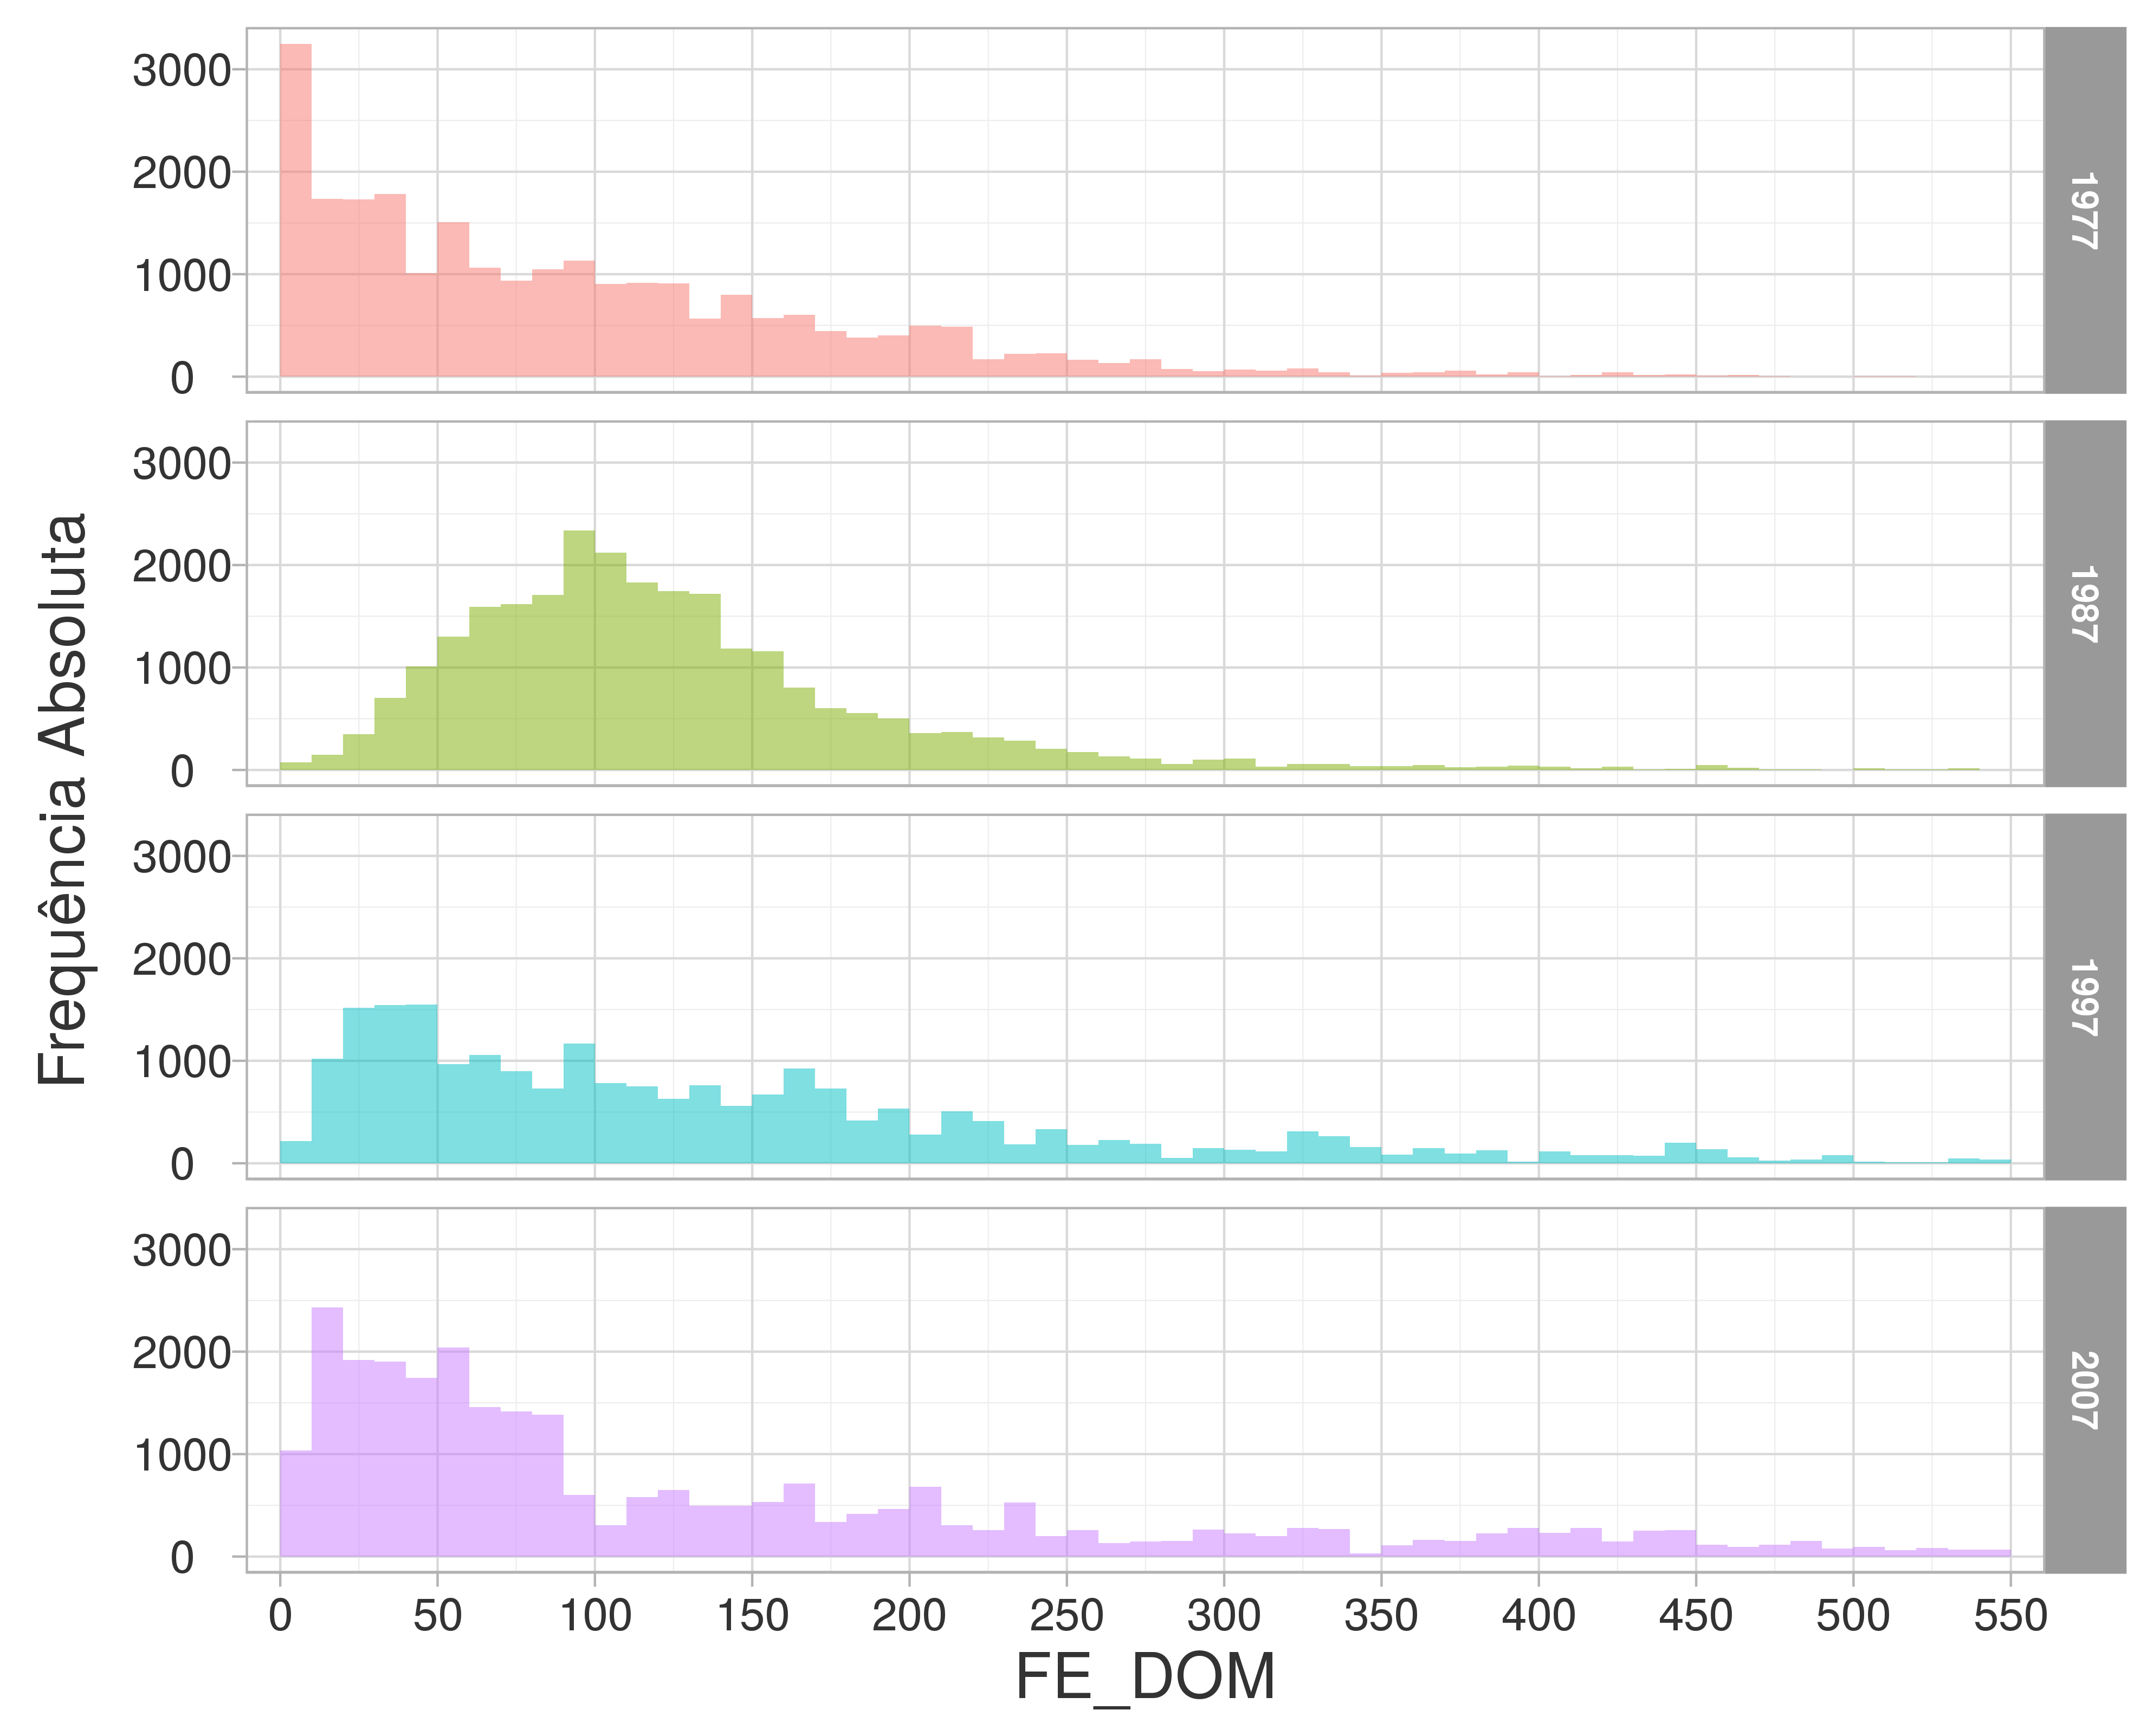
\includegraphics[width=1\textwidth]{./imagens/freq-abs-fe-dom.png}%
    \end{center}%
    %\fonte{Compilação própria}
\end{grafico}%


\clearpage

%\begin{table}[htb]
%\centering
%   \IBGEtab{%\renewcommand{\arraystretch}{1.5}%%\ABNTEXfontereduzida%
%        \renewcommand{\arraystretch}{1.5}
%        \caption{Estatísticas da variável ``FE_FAM''}
%        \label{tab:estat-fe-fam}
%    }{%
%
%    \begin{tabular}{cccccc}
%        \toprule
%        \textbf{ANO} & \textbf{Mínimo} & \textbf{1º Quartil} & \textbf{Mediana} & \textbf{3º Quartil} & \textbf{Máximo}  \\ \midrule \midrule
%        \textbf{1977}  & 0,50 & 24,77 &  68,49 & 137,90 & 1562,75 \\ \hline
%        \textbf{1987}  & 0,00 & 78,62 & 110,93 & 151,20 & 2210,00 \\ \hline
%        \textbf{1997}  & 1,00 & 49,26 & 109,54 & 200,05 & 2513,93 \\ \hline
%        \textbf{2007}  & 2,55 & 41,31 &  88,67 & 237,21 & 2256,41 \\ \hline
%        \textbf{Geral} & 0,00 & 48,00 &  99,37 & 172,85 & 2513,93 \\ \bottomrule
%        \textbf{ANO} & \textbf{Média} & \textbf{Desvio Padrão} & \textbf{Assimetria} & \textbf{Curtose} & \textbf{Nº de ``NA''}  \\ \midrule \midrule
%        \textbf{1977}  &  93,04 &  92,12 & 2,64 & 18,70 & 0 \\ \hline
%        \textbf{1987}  & 128,04 &  90,65 & 4,90 & 52,08 & 0 \\ \hline
%        \textbf{1997}  & 169,80 & 199,60 & 3,62 & 22,09 & 0 \\ \hline
%        \textbf{2007}  & 185,42 & 229,03 & 2,65 & 10,35 & 0 \\ \hline
%        \textbf{Geral} & 145,67 & 171,27 & 3,79 & 23,80 & 0 \\ \bottomrule
%        \end{tabular}
%    }
%
%\end{table}
%% Estatísticas para registros com F_FAM==1
%
%\begin{table}[htb]
%\centering
%   \IBGEtab{%\renewcommand{\arraystretch}{1.5}%%\ABNTEXfontereduzida%
%        \renewcommand{\arraystretch}{1.5}
%        \caption{Estatísticas da variável ``FE_PESS''}
%        \label{tab:estat-fe-pess}
%    }{%
%
%    \begin{tabular}{cccccc}
%        \toprule
%        \textbf{ANO} & \textbf{Mínimo} & \textbf{1º Quartil} & \textbf{Mediana} & \textbf{3º Quartil} & \textbf{Máximo}  \\ \midrule \midrule
%        \textbf{1977}  & 0,00 & 25,33 &  71,05 & 139,25 & 1562,75 \\ \hline
%        \textbf{1987}  & 0,00 & 79,46 & 111,78 & 151,24 & 2210,00 \\ \hline
%        \textbf{1997}  & 1,00 & 46,72 & 109,21 & 200,22 & 2516,28 \\ \hline
%        \textbf{2007}  & 2,92 & 48,25 & 111,45 & 296,24 & 2723,05 \\ \hline
%        \textbf{Geral} & 0,00 & 50,53 & 101,89 & 175,00 & 2723,05 \\ \bottomrule
%        \textbf{ANO} & \textbf{Média} & \textbf{Desvio Padrão} & \textbf{Assimetria} & \textbf{Curtose} & \textbf{Nº de ``NA''}  \\ \midrule \midrule
%        \textbf{1977}  &  95,10 &  94,15 & 2,76 & 20,84 & 0 \\ \hline
%        \textbf{1987}  & 128,58 &  90,56 & 4,78 & 49,15 & 0 \\ \hline
%        \textbf{1997}  & 170,00 & 203,37 & 3,69 & 23,14 & 0 \\ \hline
%        \textbf{2007}  & 213,72 & 260,38 & 2,81 & 12,60 & 0 \\ \hline
%        \textbf{Geral} & 148,76 & 177,83 & 4,14 & 29,04 & 0 \\ \bottomrule
%        \end{tabular}
%    }
%
%\end{table}
%% Estatísticas para registros com F_PESS==1

\clearpage
A variável \textbf{TIPO_DOM}, em 1977 e 1987, contava somente com as categorias particular e coletivo; já em 1997 e 2007 passou a existir também a categoria favela. Foram adotadas as categorias coletivo e particular, de forma que funcionasse como uma \textbf{dummy} indicativa de domicílio particular (1) ou não (0). Quem não respondeu foi tratado como ``NA'', encerrando 4 domicílios (23 registros) em 1987, conforme pode ser observado na Tabela \ref{tab:estat-tipo-dom}. Nota-se que o percentual de moradias unifamiliares sempre permaneceu, em média, superior a 90\%.

\begin{table}[htb]
\centering
   \IBGEtab{%\renewcommand{\arraystretch}{1.5}%%\ABNTEXfontereduzida%
        \renewcommand{\arraystretch}{1.5}
        \caption{Estatísticas da variável ``TIPO_DOM''}
        \label{tab:estat-tipo-dom}
    }{%

    \begin{tabular}{cccccc}
        \toprule
        \textbf{ANO} & \textbf{1977} & \textbf{1987} & \textbf{1997} & \textbf{2007} & \textbf{Total}\\ \midrule \midrule
        \textbf{TIPO\_DOM=0}       &    148 &    207 &  2.054 &  1.195 &   3.604 \\ \hline
        \textbf{TIPO\_DOM=1}       & 24.465 & 25.859 & 21.787 & 28.762 & 100.873 \\ \hline
        \textbf{TIPO\_DOM=``NA''}  &      0 &      4 &      0 &      0 &       4 \\ \bottomrule
        \end{tabular}
    }

\end{table}
% Estatísticas para registros com F_DOM==1

A variável \textbf{TOT_FAM}, um dado de contagem, indica quantas famílias existem no domicílio e tem suas estatísticas descritivas apresentadas na Tabela \ref{tab:estat-tot-fam}. O valor médio indica haver pouco mais de uma família por domicílio, sendo a maior média de 1997 - dado coerente com a menor porcentagem de domicílios individuais (~91\%) indicada pela variável TIPO_DOM. A Figura \ref{fig:box-plot-tot-fam} mostra que a influência dos \textit{outliers} diminui com o tempo, o que também se reflete na queda dos desvios padrão, que indica menor dispersão dos dados.


\begin{figure}[htb]%
    \caption{\label{fig:box-plot-tot-fam}Box plot da variável ``TOT_FAM'', por ano}%
    \begin{center}%
        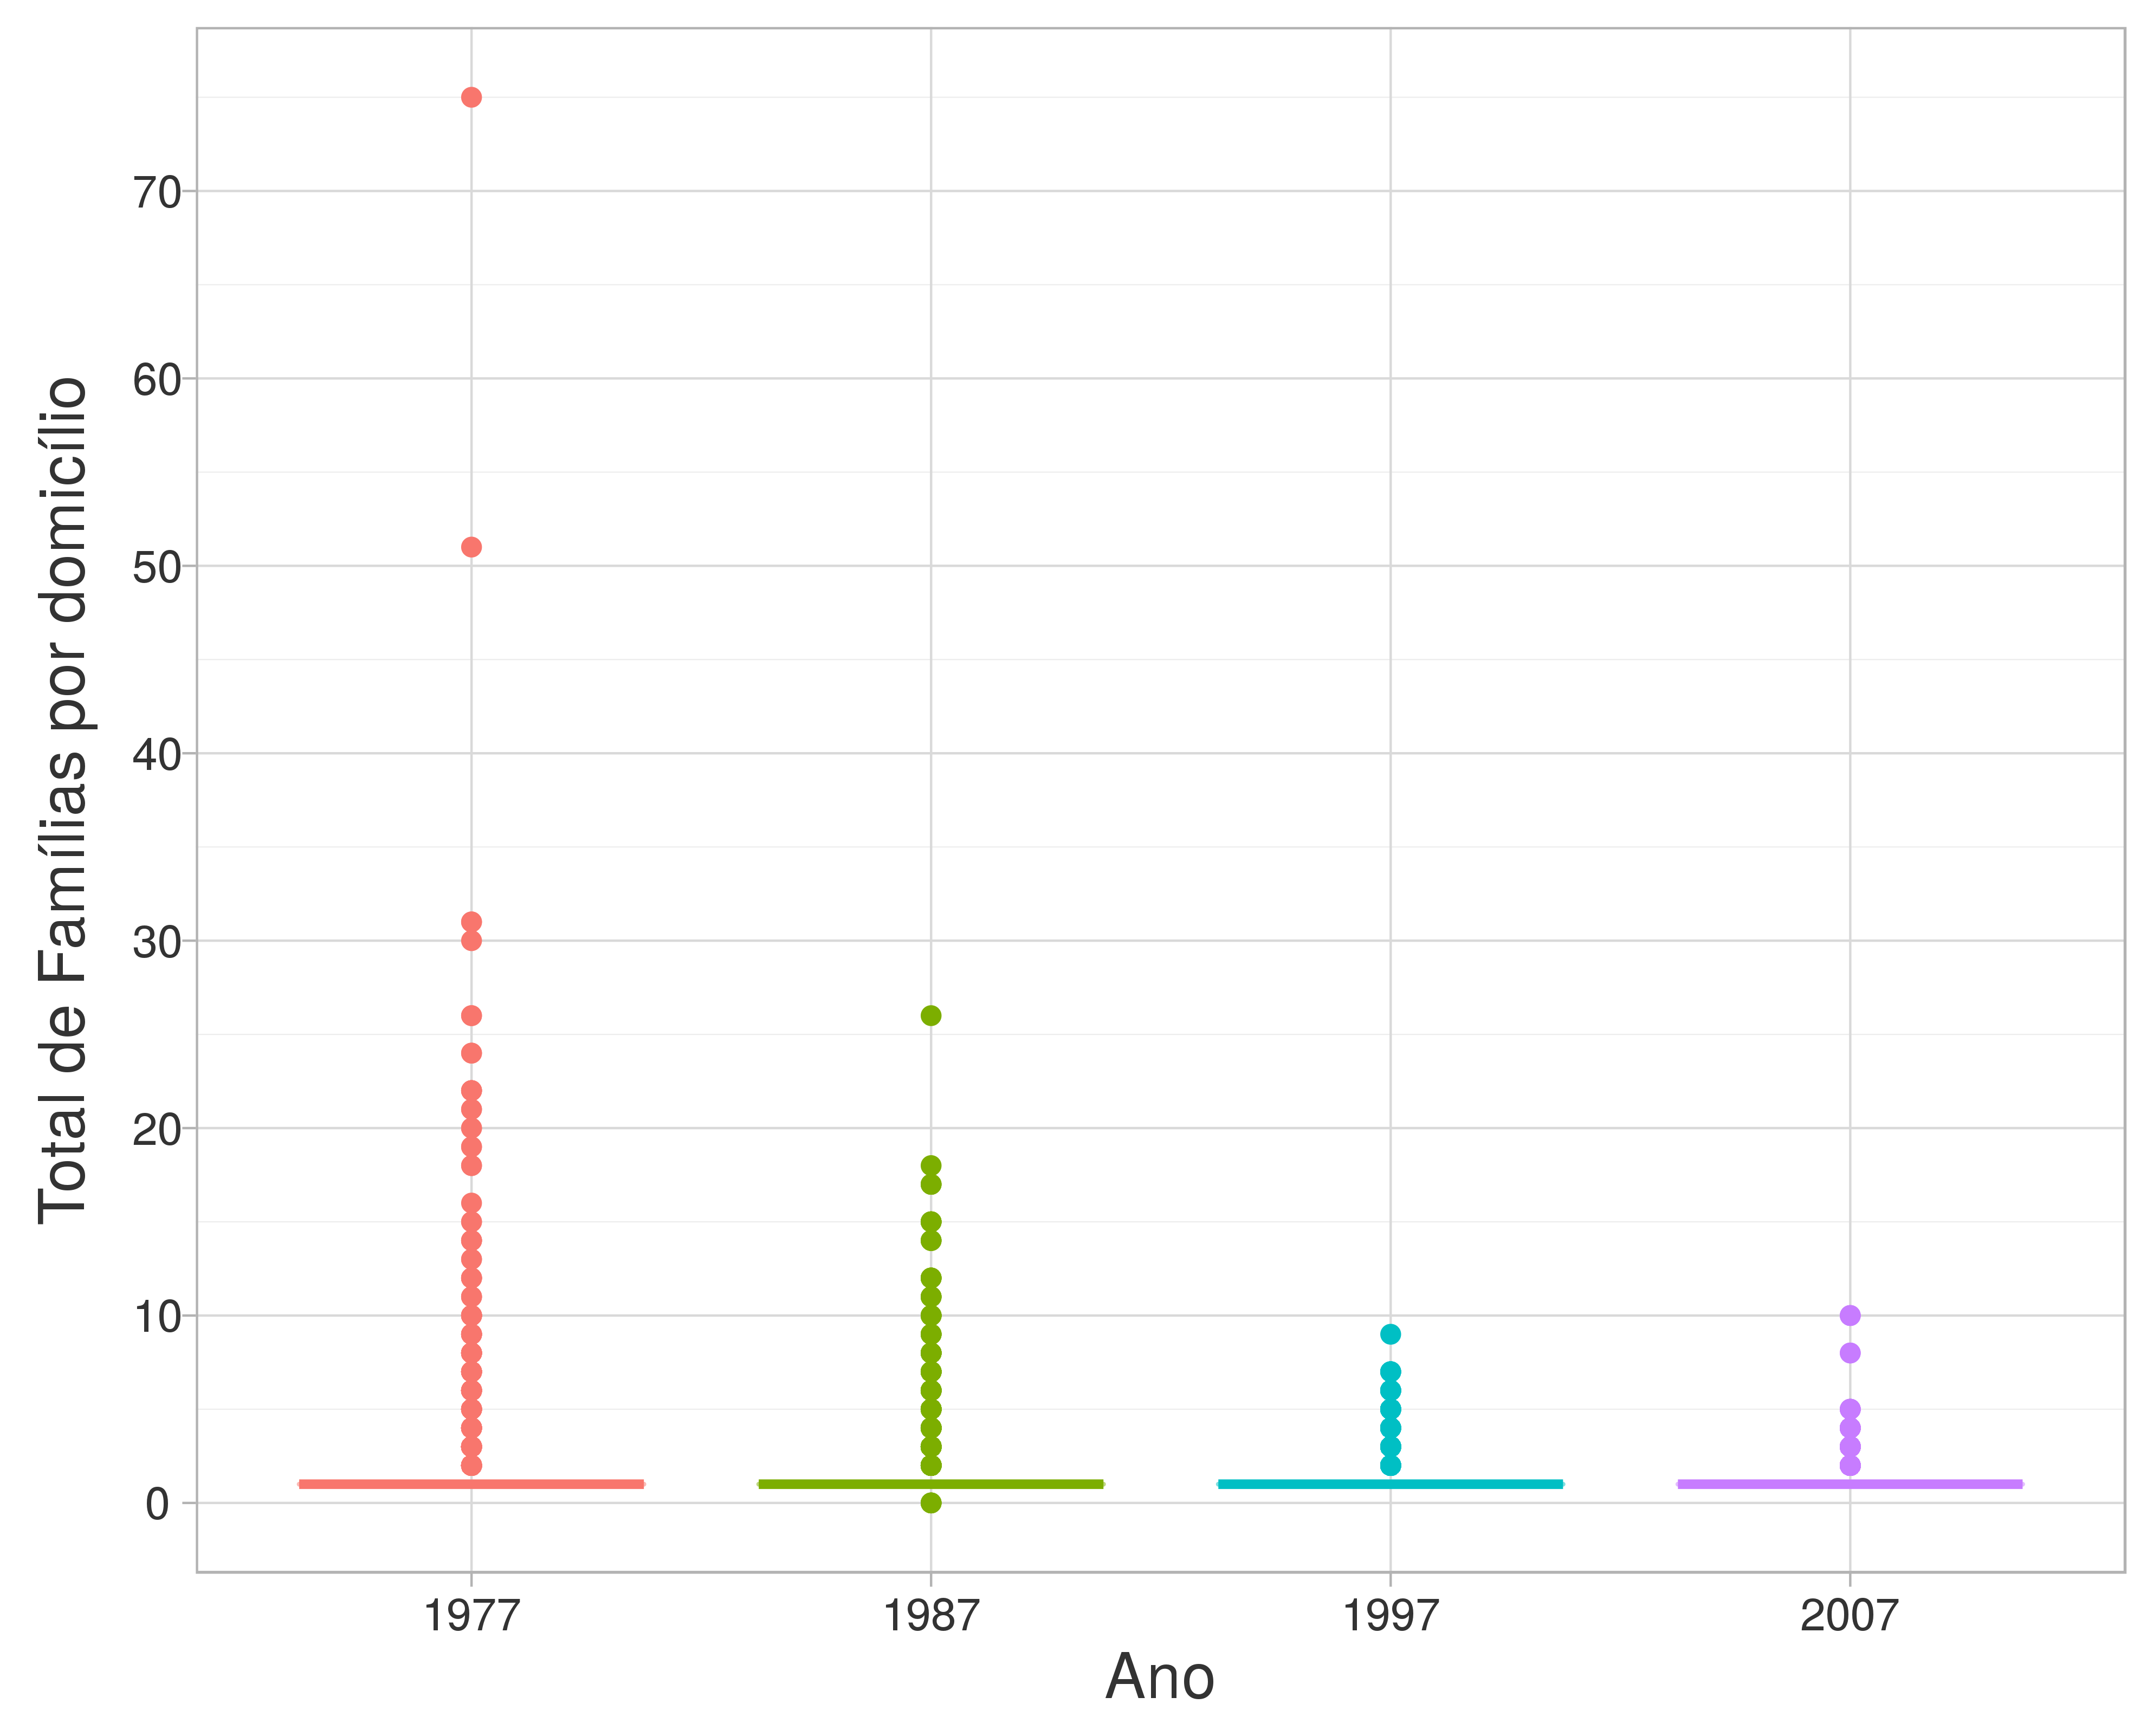
\includegraphics[width=1\textwidth]{./imagens/box-plot-tot-fam.png}%
    \end{center}%
    %\fonte{Compilação própria}
\end{figure}%

\begin{table}[htb]
\centering
   \IBGEtab{%\renewcommand{\arraystretch}{1.5}%%\ABNTEXfontereduzida%
        \renewcommand{\arraystretch}{1.5}
        \caption{Estatísticas da variável ``TOT_FAM''}
        \label{tab:estat-tot-fam}
    }{%

    \begin{tabular}{cccccc}
        \toprule
        \textbf{ANO} & \textbf{Média} & \textbf{Desvio Padrão} & \textbf{Assimetria} & \textbf{Curtose} & \textbf{Máximo}  \\ \midrule \midrule
        \textbf{1977}  & 1,08 & 0,99 & 33,70 & 1777,74 & 75 \\ \hline
        \textbf{1987}  & 1,12 & 0,61 & 13,72 & 306,37 & 26 \\ \hline
        \textbf{1997}  & 1,13 & 0,45 & 4,85 & 32,42 & 9 \\ \hline
        \textbf{2007}  & 1,03 & 0,23 & 14,00 & 346,13 & 10 \\ \hline
        \textbf{Geral} & 1,09 & 0,62 & 35,68 & 2734,92 & 75 \\ \bottomrule
        \end{tabular}
    }

\end{table}
% Estatísticas para registros com F_DOM==1


\newpage 

A variável \textbf{COND_MORA}, de natureza qualitativa, conta com três valores únicos, cujas frequências absolutas de registros são apresentada na Tabela \ref{tab:estat-cond-mora}. 
A categoria ``alugada'' (1) que em 1977 representava ~35\% da amostra, caiu para 23\% em 2007. A posse de residência (categoria ``própria'' - 2), subiu de 57\% para 68\% da amosta anual. A categoria ``outros'' (3), que abarca as categorias originais ``cedida'', ``outros'' e ``não se aplica'', oscila numa faixa próxima dos 10\%. Quem não respondeu foi tratado como ``NA'', encerrando 717 domicílios: 9 em 1977, 264 em 1987, 26 em 1997 e 460 em 2007.

\begin{table}[htb]
    \IBGEtab{%\renewcommand{\arraystretch}{1.5}%%\ABNTEXfontereduzida%
        \renewcommand{\arraystretch}{1.5}
        \caption{Estatísticas da variável ``COND_MORA''}
        \label{tab:estat-cond-mora}
    }{%

    \begin{tabular}{cccccc}
        \toprule
        \textbf{ANO} & \textbf{1977} & \textbf{1987} & \textbf{1997} & \textbf{2007} & \textbf{Total}\\ \midrule \midrule
        \textbf{COND_MORA=1}      &  9.174 &  7.967 &  5.168 &  7.268 & 29.577 \\ \hline
        \textbf{COND_MORA=2}      & 14.984 & 17.429 & 18.040 & 21.062 & 71.515 \\ \hline
        \textbf{COND_MORA=3}      &  1.990 &  2.557 &  3.611 &  1.830 &  2.065 \\ \hline
        \textbf{COND_MORA=``NA''} &      9 &    264 &     26 &    460 &    759 \\ \bottomrule
        \end{tabular}
    }

\end{table}
% Estatísticas para registros com F_FAM==1


Não foram mantidas no BDU as variáveis relativas aos bens de consumo, pois a função delas era servir de \emph{input} para determinar a renda atribuída (na ausência de declaração da renda), informação de que já se dispõe no banco de dados. Apenas os bens que são meios de transporte foram mantidos (automóveis, motocicletas e bicicletas) e serão explorados mais adiante.

Os valores monetários de renda familiar, renda individual e valor de estacionamento encontravam-se, em cada banco de dados, em um mês de referência diferente (segundo Quadro \ref{qua:atrib-renda}). Foram estudadas as possibilidades de correção pelos seguintes índices:

\begin{compactitem}
\item IPC-Brasil: índice de preços ao consumidor, que mede a variação de preços de um conjunto fixo de bens e serviços componentes de despesas habituais de famílias com nível de renda situado entre 1 e 33 salários mínimos mensais. Sua pesquisa de preços se desenvolve diariamente, cobrindo as sete principais capitais do país. Suas variações (DI, M e 10) referem-se ao período da coleta dos preços. A série histórica que se obteve de fontes oficiais (página da FGV e do Banco Central) não disponibilizava valores anteriores a 1989.

\item IGP: índice geral de preços, (a partir de 1950) é a média aritmética ponderada de três outros índices de preços (desde : Índice de Preços ao Produtor Amplo (50\%), Índice de Preços ao Consumidor (30\%) e Índice Nacional de Custo da Construção (10\%). O IGP-M/FGV se refere ao período do dia vinte e um do mês anterior ao dia vinte do mês de referência e o IGP-DI/FGV se refere ao período do dia um ao dia trinta do mês em referência. A série histórica que se obteve de fontes oficiais (página da FGV e do Banco Central) não disponibilizava valores anteriores a 1989 para o IGP-M, ao passo que o IGP-DI
\footnote{Metodologia do IGP-DI disponível em: \url{http://portalibre.fgv.br/lumis/portal/file/fileDownload.jsp?fileId=8A7C82C54DB5CA9F014DD9322ADD306E} Acesso em 30 de agosto de 2015} dispunha de valores para correção desde a década de 1940.

\item IPCA: índice geral de preços ao consumidor amplo, que mede a variação de preços de um conjunto fixo de bens e serviços componentes de despesas habituais de famílias com nível de renda situado entre 1 e 40 salários mínimos mensais. Sua pesquisa de preços se desenvolve diariamente, cobrindo as dez principais capitais do país e Brasília. A série histórica que se obteve de fontes oficiais (página do IBGE e do Banco Central) divulga valores após dezembro de 1979. Sua variação IPCA-E é ainda mais recente (1991) e tem divulgação trimestral.

\item INPC: índice nacional de preços ao consumidor amplo, que mede a variação de preços de um conjunto fixo de bens e serviços componentes de despesas habituais de famílias com nível de renda situado entre 1 e 5 salários mínimos mensais. Sua pesquisa de preços se desenvolve continuamente, cobrindo as dez principais capitais do país e Brasília. A série histórica que se obteve de fontes oficiais (página do IBGE e do Banco Central) divulga valores após março de 1979.

\end{compactitem}

Assim, pela abrangência histórica foi utilizado o IPG-DI para levar os valores de setembro de 1977 para setembro de 1987. Estes valores, bem como os advindos da OD de 1987, foram levados a outubro de 2007 sofrendo correção do INPC. Este mesmo índice foi utilizado para levar os valores de outubro de 1997 a outubro de 2007. Escolheu-se o INPC, dentro os demais disponíveis, devido à faixa de abrangência da renda familiar utilizada em sua determinação. Não se quis priorizar índices cujas cestas tivessem um perfil de consumo alto, dado que as politicas de transporte público devem priorizar especialmente as menores faixas de renda. A composição final dos deflatores utilizados é apresentada na Tabela \ref{tab:deflatores}.

\begin{table}[htb]
    \IBGEtab{%\renewcommand{\arraystretch}{1.5}%%\ABNTEXfontereduzida%
        \renewcommand{\arraystretch}{1.5}
        \caption{Deflatores utilizados para correção dos valores monetários para outubro/2007}
        \label{tab:deflatores}
    }{%

    \begin{tabular}{ccccc}
        \toprule
        \textbf{ANO} & \textbf{1977} & \textbf{1987} & \textbf{1997} & \textbf{2007}\\ \midrule \midrule
        \textbf{Deflator} & 0,44234590 & 0,09664666 & 1,94136464 & 1  \\ \bottomrule
        \end{tabular}
    }

\end{table}


A renda familiar (variável \textbf{REN_FAM}) tem seus maiores de média e mediana em 1977, conforme Tabela \ref{tab:estat-ren-fam}, talvez por reflexo da época do ``milagre econômico brasileiro'', %TODO por referencia aqui 
comumente atribuído ao período do final dos anos 1960 até a metade dos anos 1970.
Após isso, 1987 apresenta a menor média e também queda da mediana, pode ser devido à recessão que marcou o Brasil nos anos 1980, quando se registraram baixo crescimento do PIB, %TODO por referencia aqui
alto nível de desemprego, %TODO por referencia aqui
perda do poder de compra da população, %TODO por referencia aqui 
e índices de inflação extremamente elevados. %TODO por referencia aqui
Em 1997, as média da renda familiar sobe, porém a mediana continua a cair, o que pode significar uma recuperação do aquecimento econômico, porém, sem frear o aprofundamento das desigualdades. %TODO por referencia aqui
Com o valor da média de 2007, parece realmente estar ocorrendo uma recuperação econômica (aumento da renda média familiar) e também uma redução das desigualdades (aumento da mediana da renda média familiar) - ver Gráfico \ref{graf:freq-rel-ren-fam}.


\begin{table}[htb]
\centering
   \IBGEtab{%\renewcommand{\arraystretch}{1.5}%%\ABNTEXfontereduzida%
        \renewcommand{\arraystretch}{1.5}
        \caption{Estatísticas da variável ``REN_FAM''}
        \label{tab:estat-ren-fam}
    }{%
    \begin{tabular}{cccccc}
        \toprule
        \textbf{ANO} & \textbf{Mínimo} & \textbf{1º Quartil} & \textbf{Mediana} & \textbf{3º Quartil} & \textbf{Máximo}  \\ \midrule \midrule
        \textbf{1977}  & 0 & 1.351,51 & 2.534,08 & 4.796,58 &  42.234,2 \\ \hline
        \textbf{1987}  & 0 &   875,62 & 1.523,44 & 2.801,21 &  61.830,1 \\ \hline
        \textbf{1997}  & 0 &   330,03 & 1.203,65 & 2.912,05 & 172.781,0 \\ \hline
        \textbf{2007}  & 0 & 1.144,82 & 2.080,00 & 4.000,00 &  46.000,0 \\ \hline
        \textbf{Geral} & 0 &   935,73 & 1.801,63 & 3.582,21 & 172.181,0 \\ \bottomrule
        \textbf{ANO} & \textbf{Média} & \textbf{Desvio Padrão} & \textbf{Assimetria} & \textbf{Curtose} & \textbf{Nº de ``NA''}  \\ \midrule \midrule
        \textbf{1977}  & 4.037,27 & 4.724,88 & 3,56 &  18,74 & 0 \\ \hline
        \textbf{1987}  & 2.393,58 & 2.826,96 & 4,06 &  29,85 & 0 \\ \hline
        \textbf{1997}  & 2.453,89 & 4.148,06 & 7,20 & 149,78 & 0 \\ \hline
        \textbf{2007}  & 3.186,19 & 3.312,25 & 2,85 &  13,73 & 0 \\ \hline
        \textbf{Geral} & 3.009,86 & 3.845,58 & 4,74 &  63,49 & 0 \\ \bottomrule
        \end{tabular}
    }

\end{table}
% Estatísticas para registros com F_FAM==1

\begin{grafico}[htb]%
    \caption{\label{graf:freq-rel-ren-fam}Distribuição da variável ``REN_FAM'', por ano}%
    \begin{center}%
        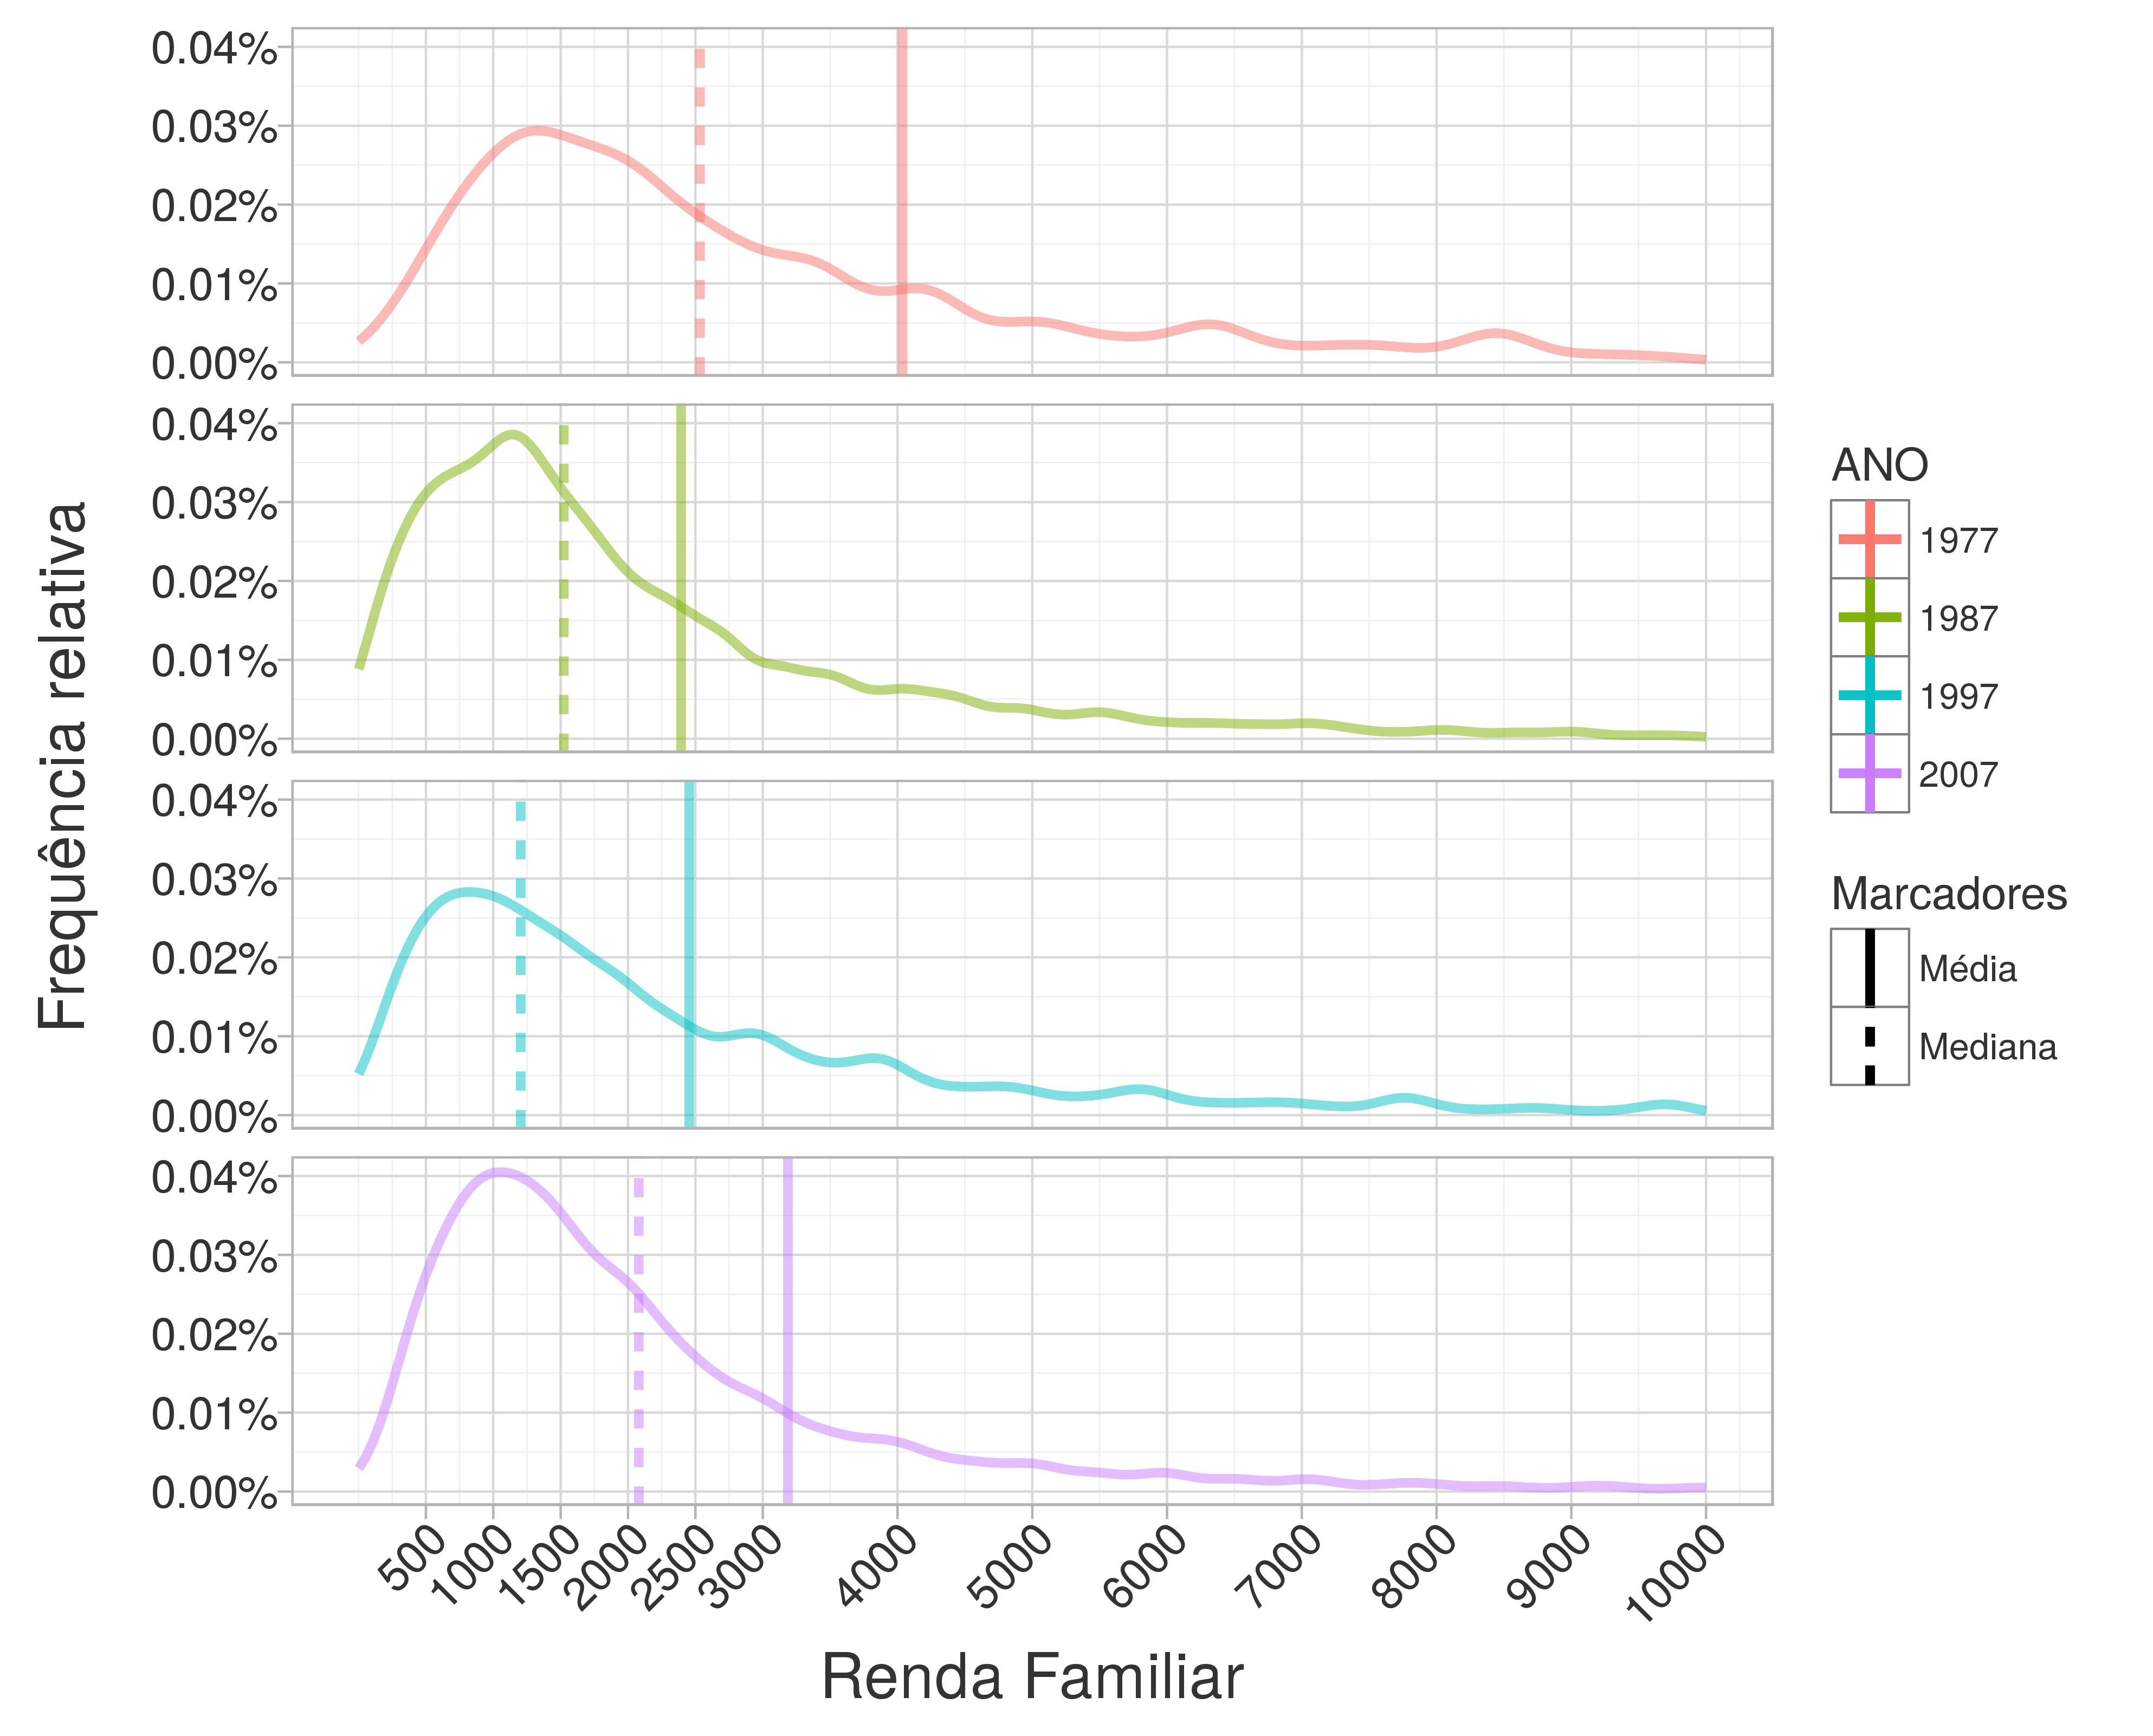
\includegraphics[width=1\textwidth]{./imagens/freq-rel-ren-fam.png}%
    \end{center}%
    %\fonte{Compilação própria}
\end{grafico}%

Para a construção do Gráfico \ref{graf:class-econ-ren-fam}, a partir da variável \textbf{FAIXA_REN_FAM}, foram retiradas as famílias que declararam renda nula. Posto isso, vê-se que as classes E e D, em 1977, correspondiam a 29\% da amostra. Em 1987 esse valor vai a 49\% e depois começa a decrescer para 45\% em 1997 e 37\% em 2007. A classe C (classe média) decresce de 1977 (~37\%) até 1997 (~33\%) e só aumenta novamente em 2007 (~36\%). Para estas classificações, foram utilizados sempre os valores em R\$ de outubro de 2007, bem como a classificação de classes econômicas vigente neste mesmo período.

\begin{grafico}[htb]%
    \caption{\label{graf:class-econ-ren-fam}Distribuição da variável ``FAIXA_REN_FAM'', por ano}%
    \begin{center}%
        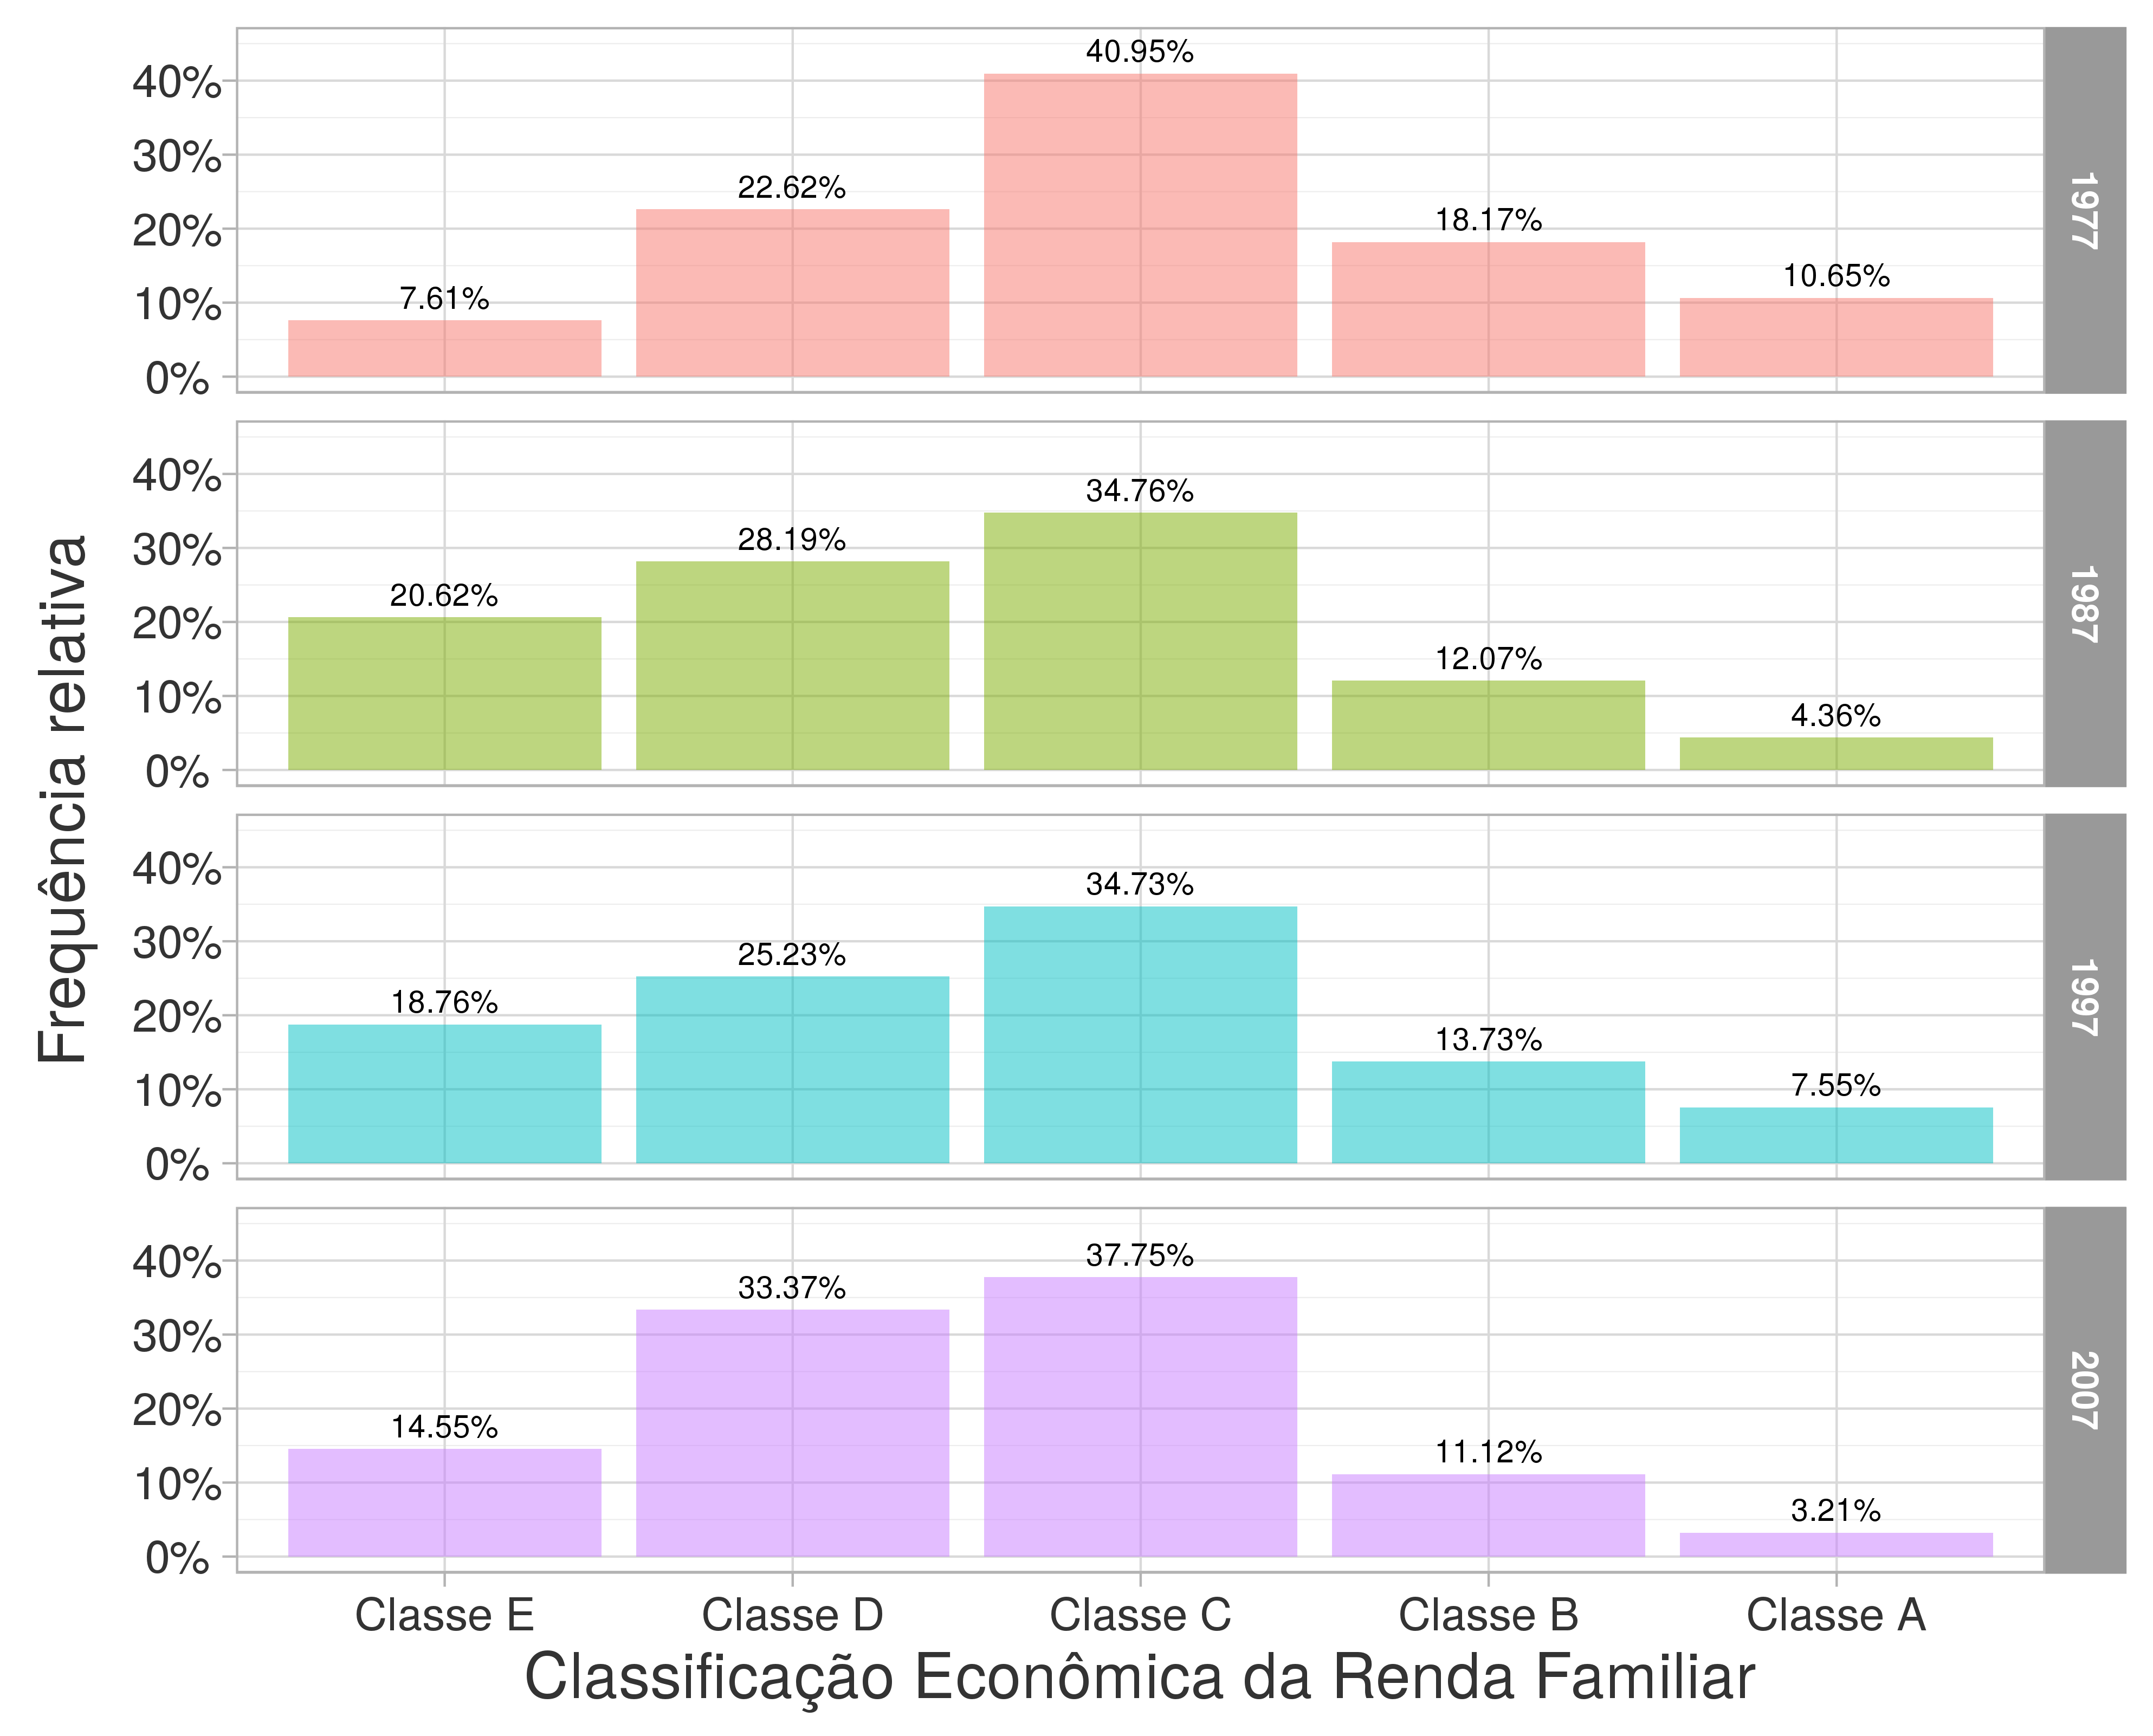
\includegraphics[width=1\textwidth]{./imagens/class-econ-ren-fam.png}%
    \end{center}%
    %\fonte{Compilação própria}
\end{grafico}%

\newpage

Uma das variáveis que são \textit{proxy} da renda é a quantidade de automóveis na família (\textbf{QT_AUTO}).
As Tabelas \ref{tab:estat-frota} e \ref{tab:venda-veic-br} mostram que a frota de automóveis de uso familiar vem crescendo tanto no Brasil como na RMSP, assim como a motorização familiar (número de veículos por família) ao longo do tempo. Isto é, mesmo com o crescimento populacional do período, a aquisição de carros pelas famílias aumenta em taxa ainda maior.
A média de automóveis por família aumentou com o passar do tempo, conforme observa-se na coluna \textit{média} da Tabela \ref{tab:estat-qt-auto}.

\begin{table}[htb]
    \IBGEtab{%\renewcommand{\arraystretch}{1.5}%%\ABNTEXfontereduzida%
        \renewcommand{\arraystretch}{1.5}
        \caption{Evolução da frota de automóveis na RMSP segundo as Pesquisas OD}
        \label{tab:estat-frota}
    }{%

    \begin{tabular}{ccccc}
        \toprule
        \textbf{ANO} & \textbf{1977} & \textbf{1987} & \textbf{1997} & \textbf{2007}\\ \midrule \midrule
        \textbf{Frota} & 1.391.832 & 2.014.474 & 3.092.238 & 3.545.263  \\ \bottomrule
        \end{tabular}
    }

    \nota{Segundo o Departamento Estadual de Trânsito de São Paulo, em 2007 o município de São Paulo contava com cerca de 4,5milhões de automóveis (Fonte: \url{http://www.detran.sp.gov.br/wps/wcm/connect/1eb3cf81-624b-4a71-b626-317730638e74/\%28Frota\%2B2008\%29.pdf?MOD=AJPERES&CACHEID=1eb3cf81-624b-4a71-b626-317730638e74}). Tal discrepância pode ocorrer porque as Pesquisas OD domiciliares tem seu número de viagens aferido (FE_VIAG deduzido) pelas viagens feitas realizadas nos sistemas de transportes de massa.}
    
\end{table}

\begin{table}[htb]
    \IBGEtab{%\renewcommand{\arraystretch}{1.5}%%\ABNTEXfontereduzida%
	    \renewcommand{\arraystretch}{1.5}
        \caption{Venda interna de veículos no Brasil entre 1960 e 2009}
		\label{tab:venda-veic-br}
    }{%
	    \begin{tabular}{p{2.00cm} P{4.0cm} P{4.0cm} P{4.0cm}}
            \toprule
	           \headerTabCenterCell{Ano} &
		       \headerCell{Autos} &
		       \headerCell{Total} &
		       \headerCell{Fator de crescimento (total)} \\
		    \midrule \midrule
		        1960&
		        40.980&
		        131.499&
		        1\\
		    \midrule
		        1970&
		        308.024&
		        416.704&
		        3,2\\
		    \midrule
		        1980&
		        739.028&
		        980.261&
		        7,5\\
		    \midrule
		        1990&
		        532.906&
		        712.741&
		        5,4\\
		    \midrule
		        2000&
		        1.176.774&
		        1.489.481&
		        11,3\\
		    \midrule
		        2009&
		        2.474.764&
		        3.141.240&
		        23,9\\
		    \bottomrule
		\end{tabular}
    }{%
		\fonte{Adaptado de \cite[p.29]{VASCONCELLOS2012}}
		}
\end{table}


\begin{table}[htb]
\centering
   \IBGEtab{%\renewcommand{\arraystretch}{1.5}%%\ABNTEXfontereduzida%
        \renewcommand{\arraystretch}{1.5}
        \caption{Estatísticas da variável ``QT_AUTO''}
        \label{tab:estat-qt-auto}
    }{%

    \begin{tabular}{cccccc}
        \toprule
        \textbf{ANO} & \textbf{Mínimo} & \textbf{1º Quartil} & \textbf{Mediana} & \textbf{3º Quartil} & \textbf{Máximo}  \\ \midrule \midrule
        \textbf{1977}  & 0 & 0 & 0 & 1 & 7 \\ \hline
        \textbf{1987}  & 0 & 0 & 0 & 1 & 9 \\ \hline
        \textbf{1997}  & 0 & 0 & 1 & 1 & 9 \\ \hline
        \textbf{2007}  & 0 & 0 & 1 & 1 & 8 \\ \hline
        \textbf{Geral} & 0 & 0 & 0 & 1 & 9 \\ \bottomrule
        \textbf{ANO} & \textbf{Média} & \textbf{Desvio Padrão} & \textbf{Assimetria} & \textbf{Curtose} & \textbf{Nº de ``NA''}  \\ \midrule \midrule
        \textbf{1977}  & 0,65 & 0,81 & 1,36 & 2,28 & 0 \\ \hline
        \textbf{1987}  & 0,57 & 0,77 & 1,59 & 4,09 & 0 \\ \hline
        \textbf{1997}  & 0,72 & 0,89 & 1,57 & 3,78 & 0 \\ \hline
        \textbf{2007}  & 0,78 & 0,86 & 1,19 & 1,99 & 0 \\ \hline
        \textbf{Geral} & 0,68 & 0,84 & 1,43 & 3,03 & 0 \\ \bottomrule
        \end{tabular}
    }

\end{table}
% Estatísticas para registros com F_FAM==1

Diversos estudos foram realizados para a construção de modelos desagregados que explicassem a posse de autos
\cite{RYAN1999, DARGAY1999, DARGAY2001, CHU2002, KARLAFTIS2002, PFEIFFER2005}.
É comum a utilização de variáveis como renda, número de trabalhadores, tamanho da família, número de estudantes, presença ou não de crianças na família, sexo e idade da pessoa responsável pela família. Embora não seja o foco deste estudo modelar a posse de autos pelas famílias, compreender o que influencia a motorização é importante porque a motorização influencia diretamente a mobilidade dos indivíduos.
\citeauthoronline{PFEIFFER2005} (\citeyear{PFEIFFER2005}), que analisam a evolução da motorização da RMSP entre 1987 e 1997, concluem que, para explicar a posse de autos ``\textit{as variáveis de estrutura familiar utilizadas na análise e modelagem da posse de autos perderam importância ao longo do tempo, assim como a própria renda familiar}''. Eles sugerem que isso pode ter de dado pela maior facilidade de financiamentos para aquisição de automóveis por uma família, ou ainda pela evolução das condições do transporte público, assim como da organização espacial da região metropolitana.

Segundo a Tabela \ref{tab:distr-autos-fam}, percebe-se que a proporção de famílias sem automóvel particular oscilou entre os anos, mantendo ainda assim um tendência de queda entre 1977 e 2007. Oscilação entre os anos também ocorreu na proporção das famílias com dois ou mais automóveis, com tendência de crescimento entre 1977 e 2007. O comportamento mais consistente com os cenários macro econômicos brasileiros foi o das famílias com um automóvel: tiveram leve queda na posse de um automóvel em 1987 (década de crise econômica), aumento de pouco mais de 10\% em 1997 (após a estabilização da moeda em 1994), e aumento tímido (0,3\%) em 2007.

As \textit{dummies} relativas à presença de automóveis na famílias foram divididas em: (i) presença de 1 automóvel e (ii) presença de 2 ou mais automóveis.
Segmentando as famílias segundo o sexo da pessoa responsável e analisando as frequências relativas da posse de auto através dessas \textit{dummies}, obtém-se o Gráfico \ref{graf:autos-sit-fam-sexo}. Nele, observa-se que as variações das taxas de motorização das famílias chefiadas por homens ou por mulheres são semelhantes, porém, as famílias da amostra com 2 ou mais automóveis, cujos responsáveis são homens, tiveram uma leve queda de 2 pontos percentuais.
Ademais, as famílias chefiadas por mulheres apresentam taxas de motorização ligeiramente mais altas (2\%) do que aquelas chefiadas por homens.
  
\begin{table}[htb]
    \IBGEtab{%\renewcommand{\arraystretch}{1.5}%%\ABNTEXfontereduzida%
        \renewcommand{\arraystretch}{1.5}
        \caption{Proporção das famílias segundo posse de automóveis}
        \label{tab:distr-autos-fam}
    }{%

    \begin{tabular}{ccccc}
        \toprule
        \textbf{ANO} & \textbf{1977} & \textbf{1987} & \textbf{1997} & \textbf{2007}\\ \midrule \midrule
        \textbf{\% de famílias sem auto} & 55,7 & 56,9 & 49,4 & 51,3  \\ \midrule
        \textbf{\% de famílias com 1 auto} & 34,1 & 33,0  & 37,3 & 37,6  \\ \midrule
        \textbf{\% de famílias com 2 ou mais autos} & 10,2 & 10,1 & 13,3 & 11,1 \\ \bottomrule
        \end{tabular}
    }

\end{table}
% Estatísticas para registros com F_FAM==1

\begin{grafico}[htb]%
    \caption{\label{graf:autos-sit-fam-sexo} Proporção de famílias com pessoa responsável do sexo feminino e do sexo masculino, segundo posse de automóveis, por ano}%
    \begin{center}%
        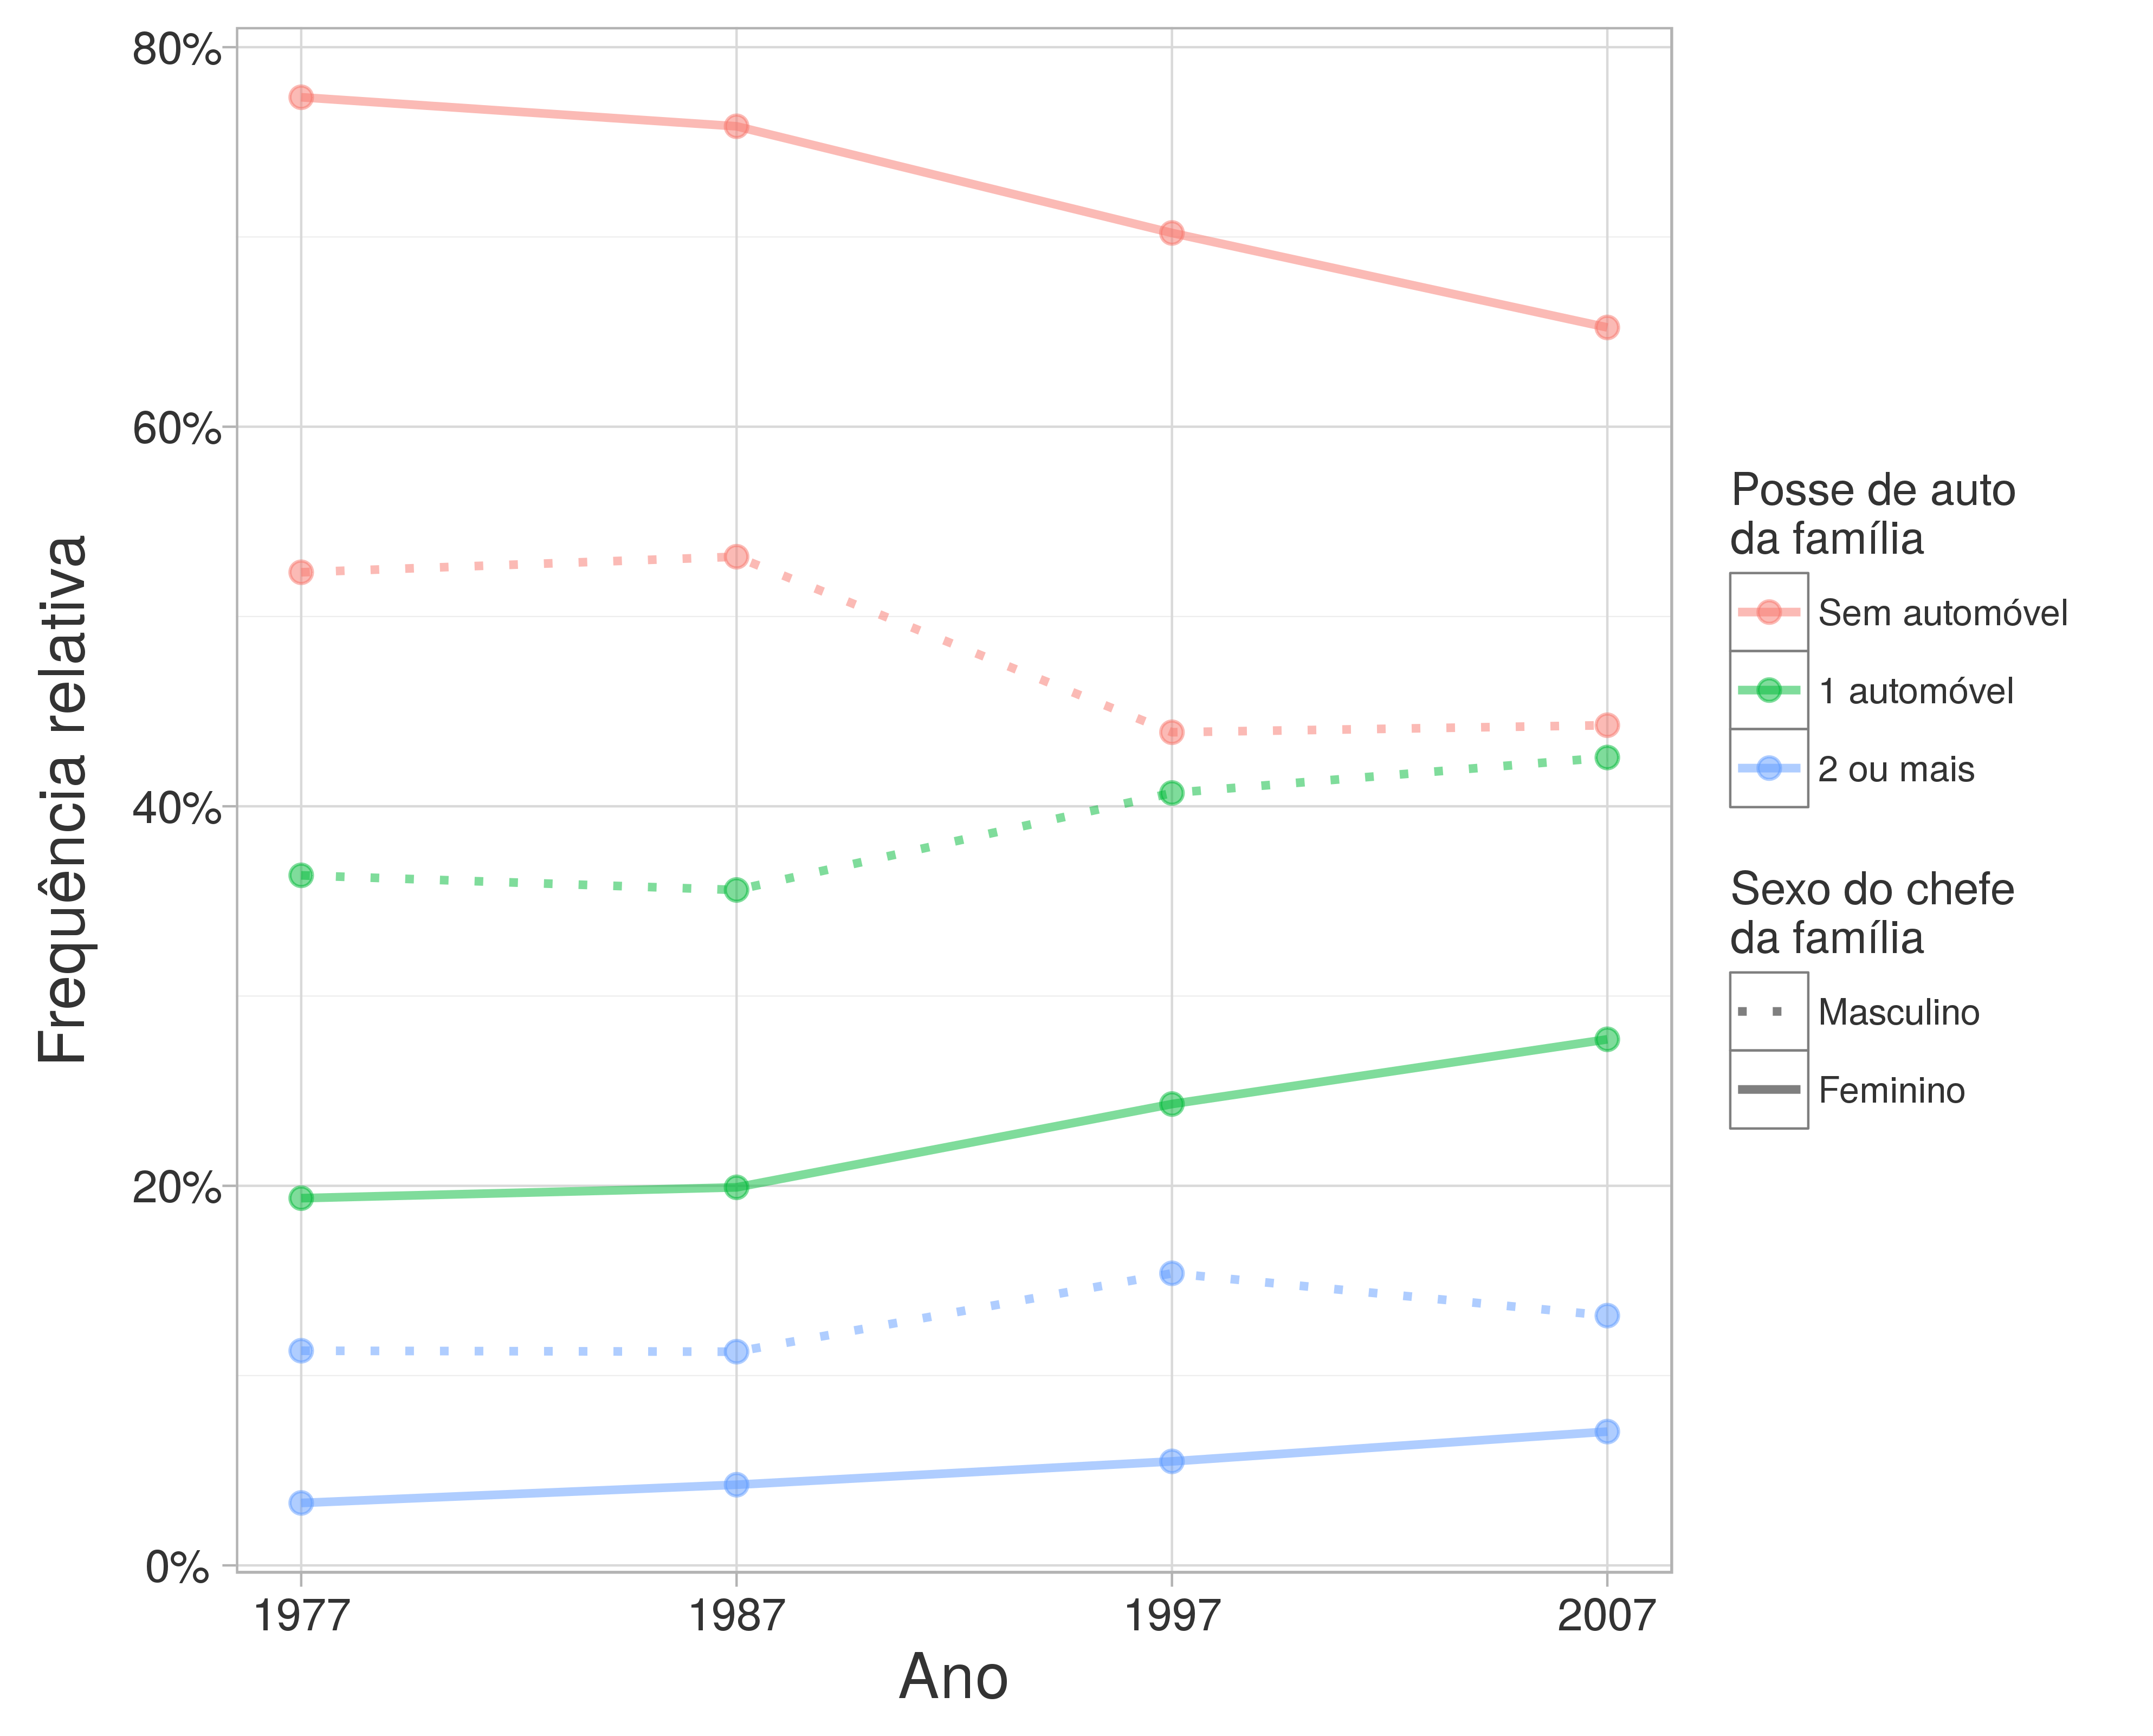
\includegraphics[width=1\textwidth]{./imagens/autos-sit-fam-sexo.png}%
    \end{center}%
    %\fonte{Compilação própria}
\end{grafico}%


A quantidade de motocicletas (\textbf{QT_MOTO}) e bicicletas (\textbf{QT_BICI}) foram levantadas apenas na Pesquisa OD de 2007, e tem suas estatísticas descritivas são apresentadas na Tabela \ref{tab:estat-qt-moto-bici}.
Percebe-se que, embora um meio de transporte individual motorizado mais barato, a incidência da posse de motocicletas é uma fenômeno mais raro, provavelmente devido ao risco associado a esse meio de transporte
\footnote{Segundo dados da CET o índice de acidentes com motociclistas...}. 
%TODO preencher nota de rodapé

Essa falta de segurança na condução do meio de transporte também ocorre com a bicicleta, porém, além de ser ainda mais barata que a motocicleta, ela não é motorizada e, por isso, comumente trafega nos passeios públicos e calçadas, onde o(a) condutor(a) sofre menor risco de colisão com meios motorizados de transporte (motocicletas, carros, ônibus e caminhões). Com a recente política municipal de incentivo à bicicleta como meio de transporte, por meio de investimentos em infraestrutura cicloviária, é possível que na Pesquisa OD de 2017 haja evoluções destes dados que mereçam investigação.
Vale lembrar que existe também a questão do status associado muito mais fortemente à posse do automóvel do que da motocicleta; e no caso das bicicletas, seu uso é associado à ideia de pobreza e falta de recursos suficientes para comprar um carro.
%TODO por referências aqui

\begin{table}[htb]
\centering
   \IBGEtab{%\renewcommand{\arraystretch}{1.5}%%\ABNTEXfontereduzida%
        \renewcommand{\arraystretch}{1.5}
        \caption{Estatísticas das variáveis ``QT_MOTO'' e ``QT_BICI''}
        \label{tab:estat-qt-moto-bici}
    }{%

    \begin{tabular}{cccccc}
        \toprule
        \textbf{2007} & \textbf{Mínimo} & \textbf{1º Quartil} & \textbf{Mediana} & \textbf{3º Quartil} & \textbf{Máximo}  \\ \midrule \midrule
        \textbf{motocicleta}  &  0 &  0 &  0 &  0 &  9 \\ \hline
        \textbf{bicicleta} &  0 &  0 &  0 &  1 &  9 \\ \bottomrule
        \textbf{ANO} & \textbf{Média} & \textbf{Desvio Padrão} & \textbf{Assimetria} & \textbf{Curtose} & \textbf{Nº de ``NA''}  \\ \midrule \midrule
        \textbf{motocicleta}  & 0,07 & 0,29 & 5,86 & 74,31 &      0 \\ \hline
        \textbf{bicicleta} & 0,46 & 0,8 & 2,27 & 7,5 & 0 \\ \bottomrule
        \end{tabular}
    }

\end{table}
% Estatísticas para registros com F_FAM==1

A variável \textbf{TOT_PESS}, um dado de contagem, indica quantas pessoas existem na família e tem suas estatísticas descritivas apresentadas na Tabela \ref{tab:estat-tot-pess}. Não haviam \textit{missing values} e o valor médio indica que o tamanho da família diminuiu, passando de pouco mais de 4 pessoas em 1977 para pouco menos de 3 pessoas por família em 2007.
Em comportamento análogo a TOT_FAM, a Figura \ref{fig:box-plot-tot-pess} indica que a influência dos \textit{outliers} de TOT_PESS diminui com o tempo, o que também se reflete na queda dos desvios padrão, que indica menor dispersão dos dados.

\begin{table}[htb]
\centering
   \IBGEtab{%\renewcommand{\arraystretch}{1.5}%%\ABNTEXfontereduzida%
        \renewcommand{\arraystretch}{1.5}
        \caption{Estatísticas da variável ``TOT_PESS''}
        \label{tab:estat-tot-pess}
    }{%

    \begin{tabular}{cccccc}
        \toprule
        \textbf{ANO} & \textbf{Média} & \textbf{Desvio Padrão} & \textbf{Assimetria} & \textbf{Curtose} & \textbf{Máximo}  \\ \midrule \midrule
        \textbf{1977}  & 4,13 & 2,09 & 0,99 & 1,78 & 18 \\ \hline
        \textbf{1987}  & 3,93 & 1,80 & 0,92 & 2,03 & 22 \\ \hline
        \textbf{1997}  & 3,68 & 1,73 & 0,82 & 1,68 & 17 \\ \hline
        \textbf{2007}  & 2,96 & 1,46 & 0,78 & 1,00 & 14 \\ \hline
        \textbf{Geral} & 3,65 & 1,83 & 1,00 & 2,10 & 22 \\ \bottomrule
        \end{tabular}
    }

\end{table}
% Estatísticas para registros com F_FAM==1


\begin{figure}[htb]%
    \caption{\label{fig:box-plot-tot-pess}Box plot da variável ``TOT_PESS'', por ano}%
    \begin{center}%
        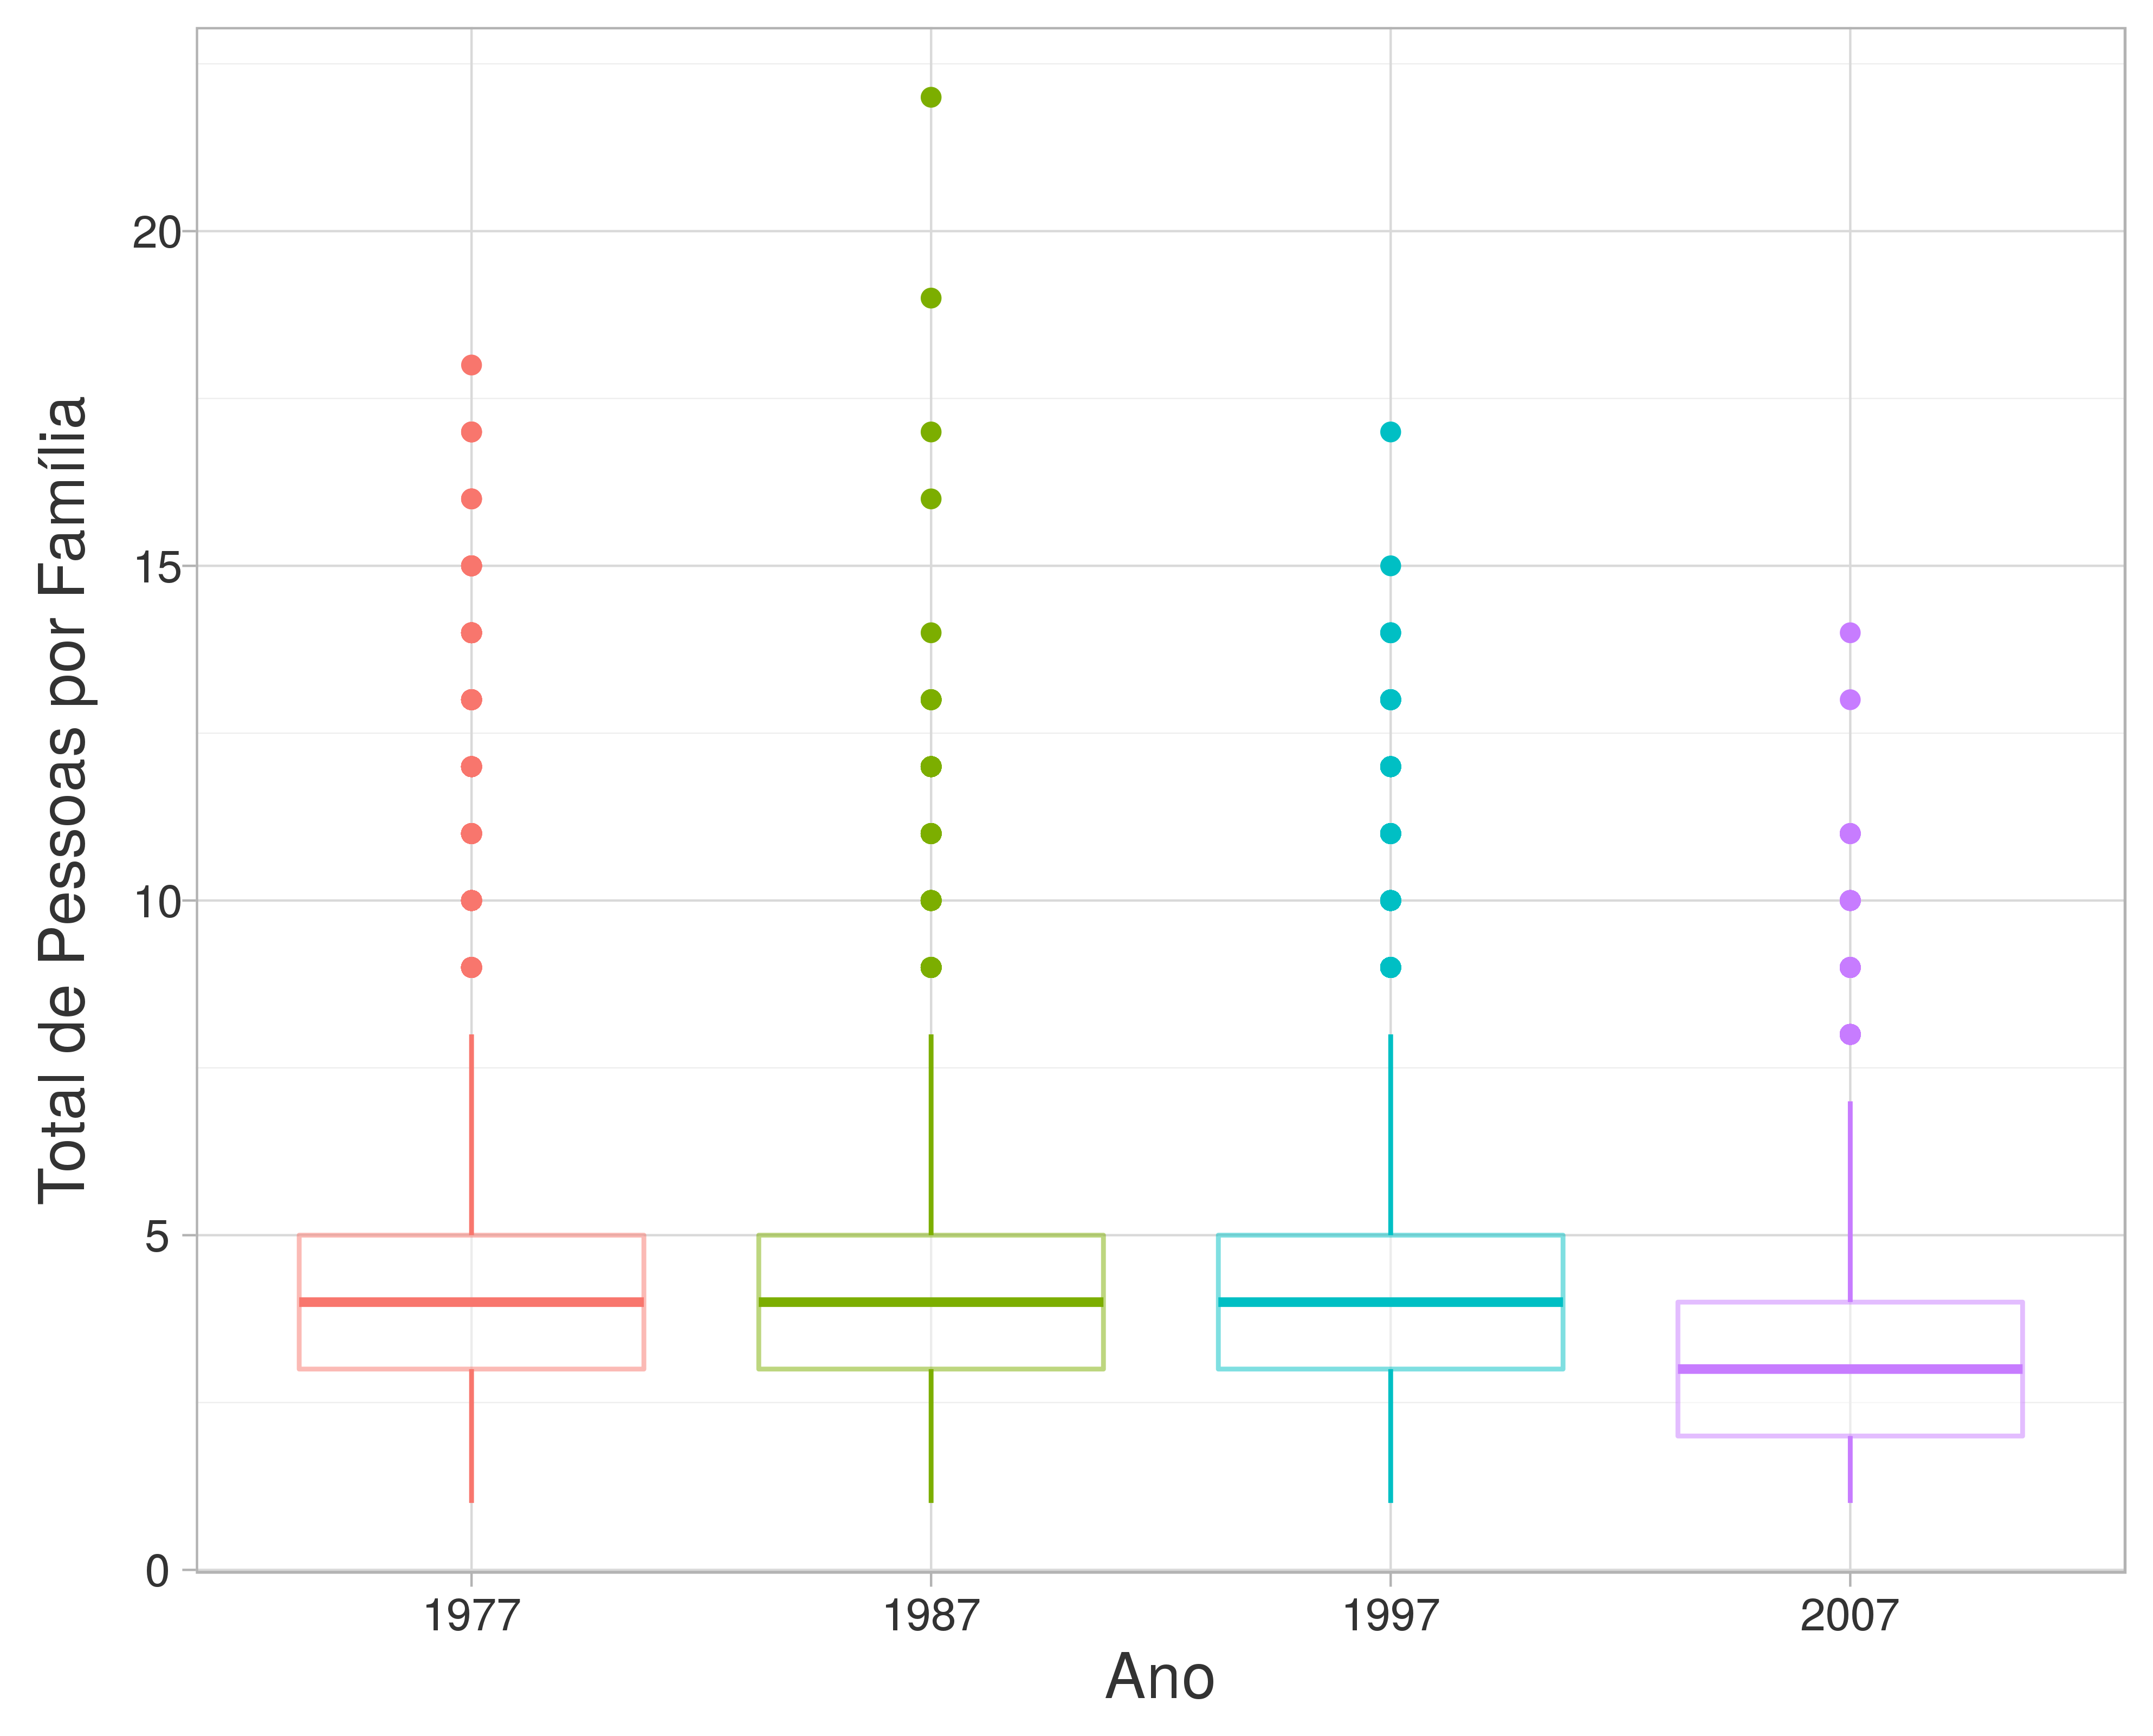
\includegraphics[width=1\textwidth]{./imagens/box-plot-tot-pess.png}%
    \end{center}%
    %\fonte{Compilação própria}
\end{figure}%

Percebe-se pelo Gráfico \ref{graf:pres-flh-idoso-fam} a tendência de diminuição geral nas porcentagens de famílias com filhos pequenos (até 9 anos) a partir de 1987, efeito que será percebido na faixa etária seguinte (entre 10 e 19 anos) em 1997. Essa diminuição da presença de dependentes jovens (crianças/adolescentes) mantém-se em 2007. Nos mesmos períodos de análise, ocorre o envelhecimento da população, efeito capturado no gráfico pela presença de idosos (acima de 60 ou de 70 anos) com taxas positivas de crescimento.

\begin{grafico}[htb]%
    \caption{\label{graf:pres-flh-idoso-fam}Proporção de famílias com presença de dependentes, por ano}%
    \begin{center}%
        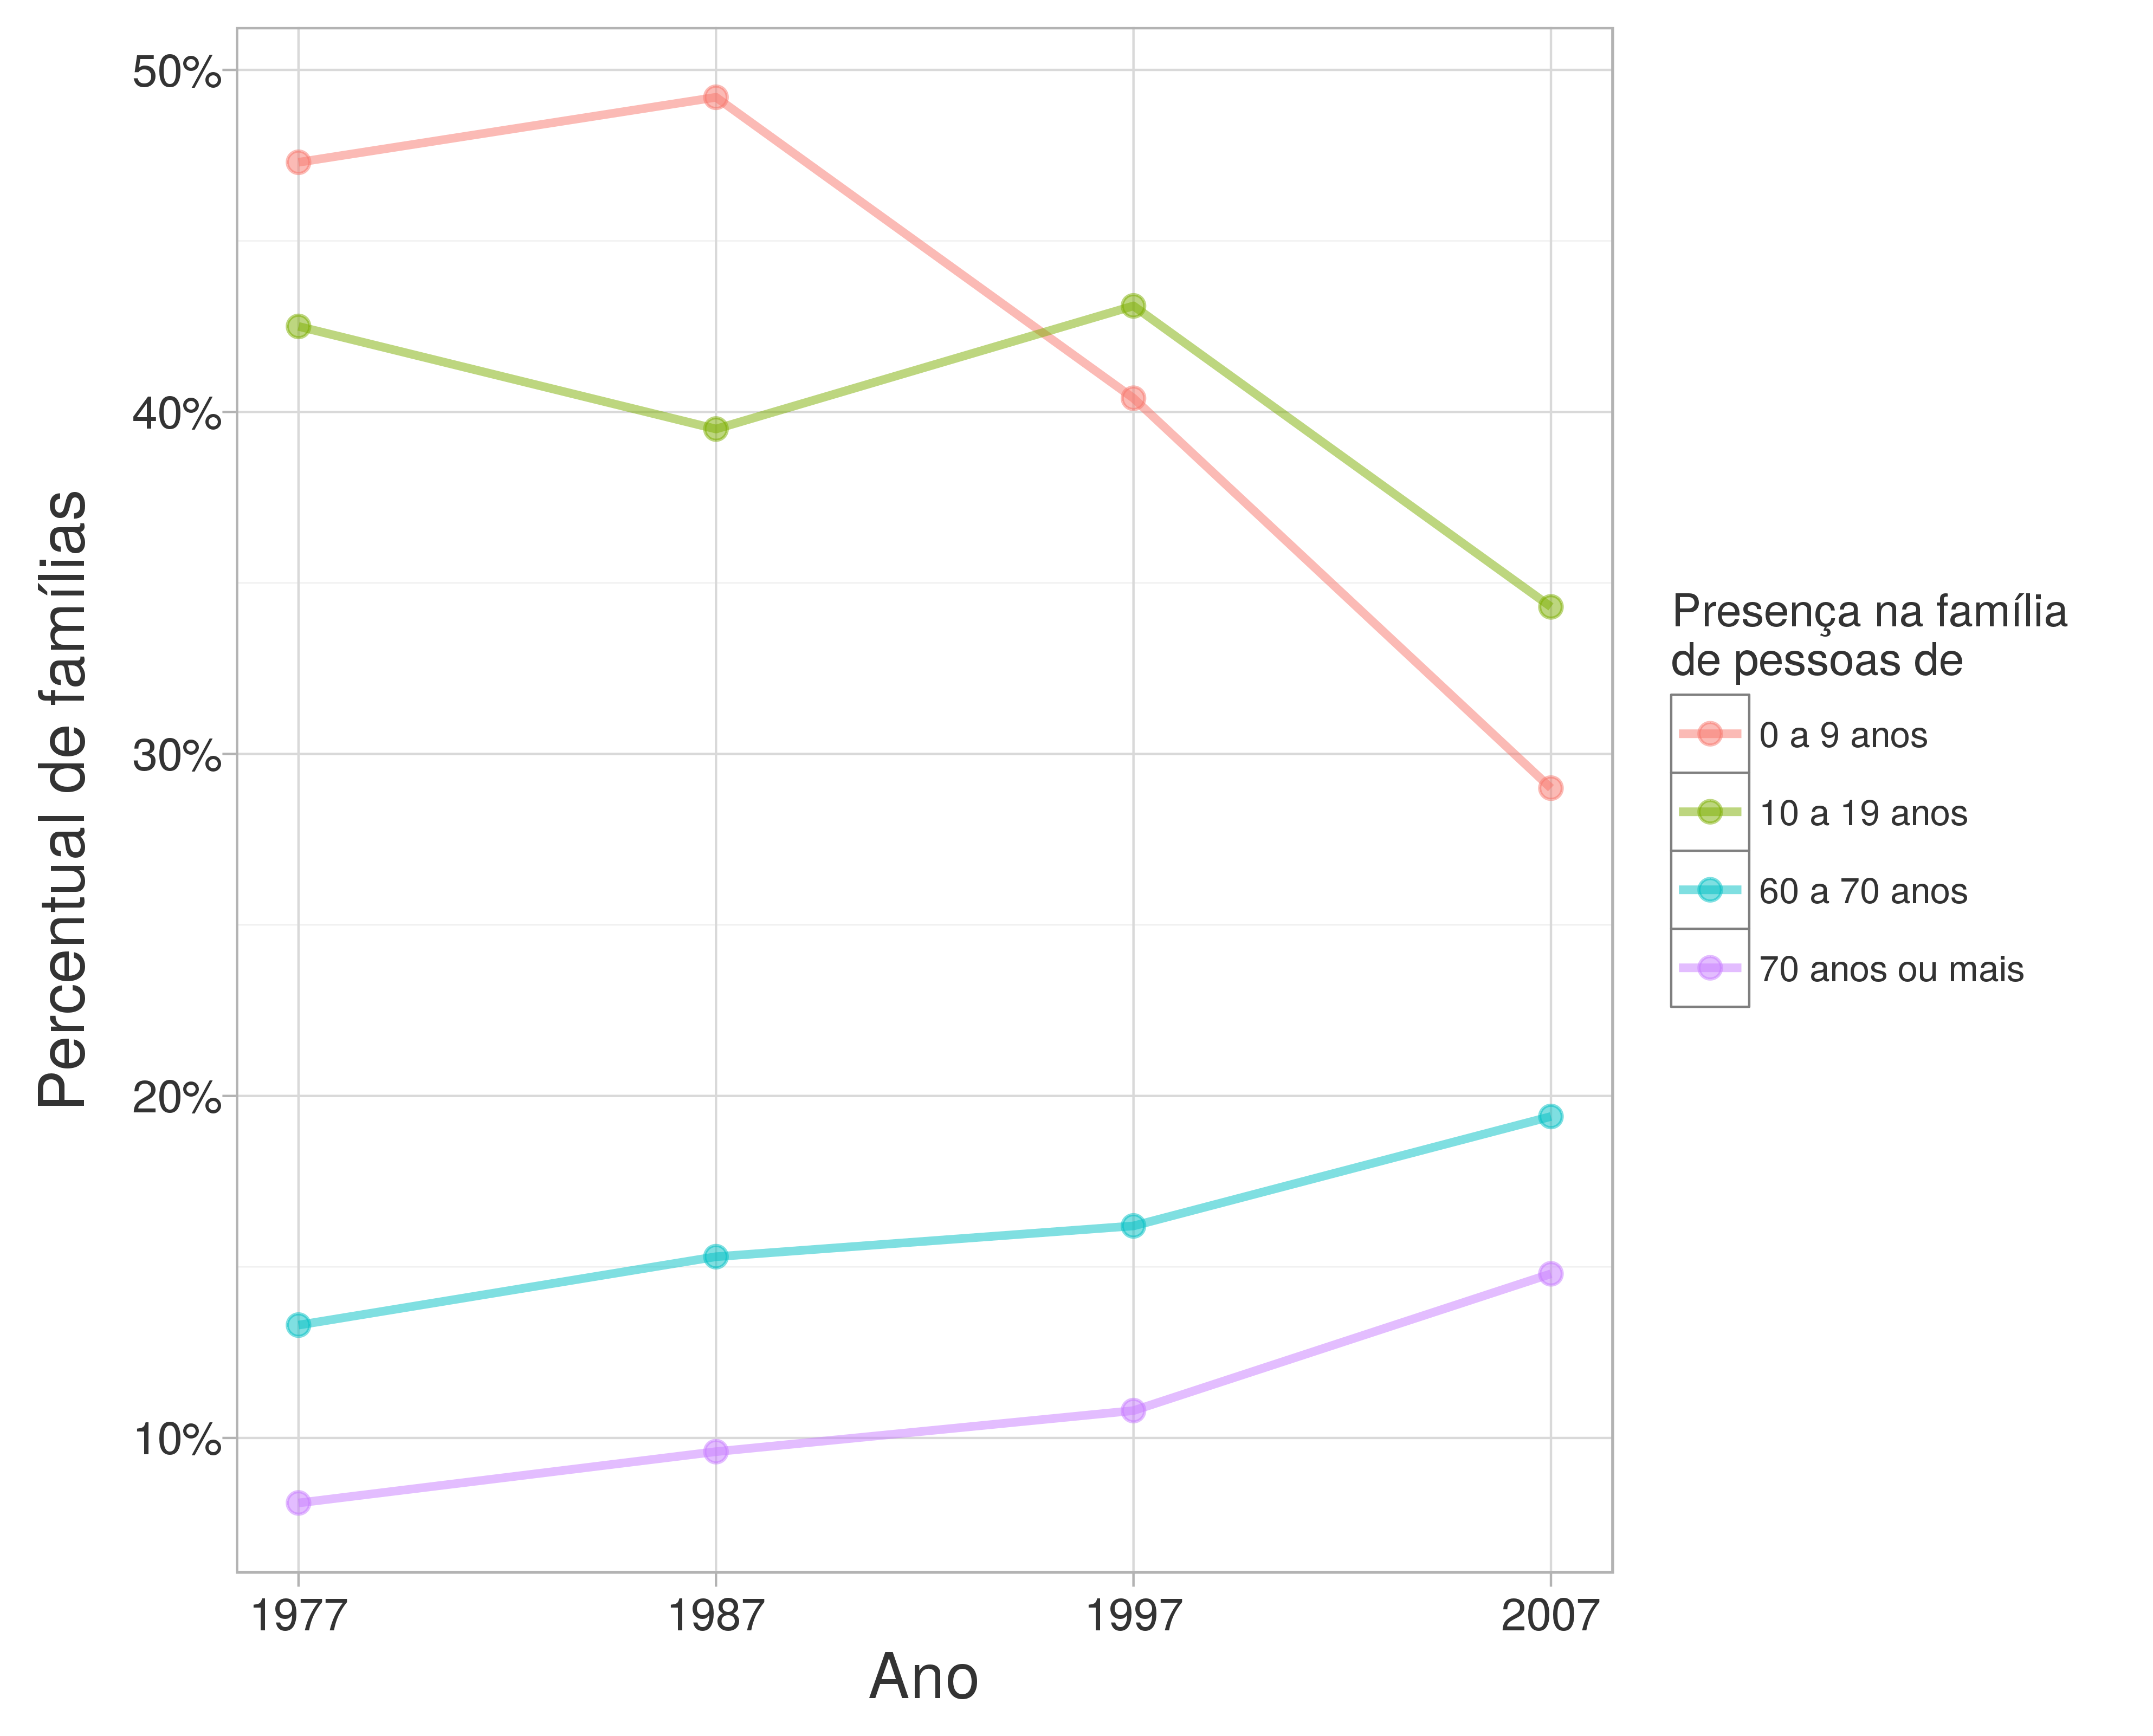
\includegraphics[width=1\textwidth]{./imagens/pres-flh-idoso-fam.png}%
    \end{center}%
    %\fonte{Compilação própria}
\end{grafico}%

Como um dos fatores do indivíduo que influencia seu padrão de deslocamentos está o estágio no ``ciclo de vida'' \cite{BILT1997}.
Isto é, as atividades desenvolvidas por uma pessoa depende em que fase da vida ela, e também os demais membros da família, se encontram. A variável \textbf{IDADE} é uma das variáveis que definem o ciclo de vida das pessoas. É possível perceber no Gráfico \ref{graf:distr-idade} que houve uma transição da pirâmide etária da RMSP, indicando envelhecimento da população tanto masculina como feminina.

\begin{grafico}[htb]%
    \caption{\label{graf:distr-idade}Distribuição da variável ``IDADE'' de respondentes, por ano e por sexo}%
    \begin{center}%
        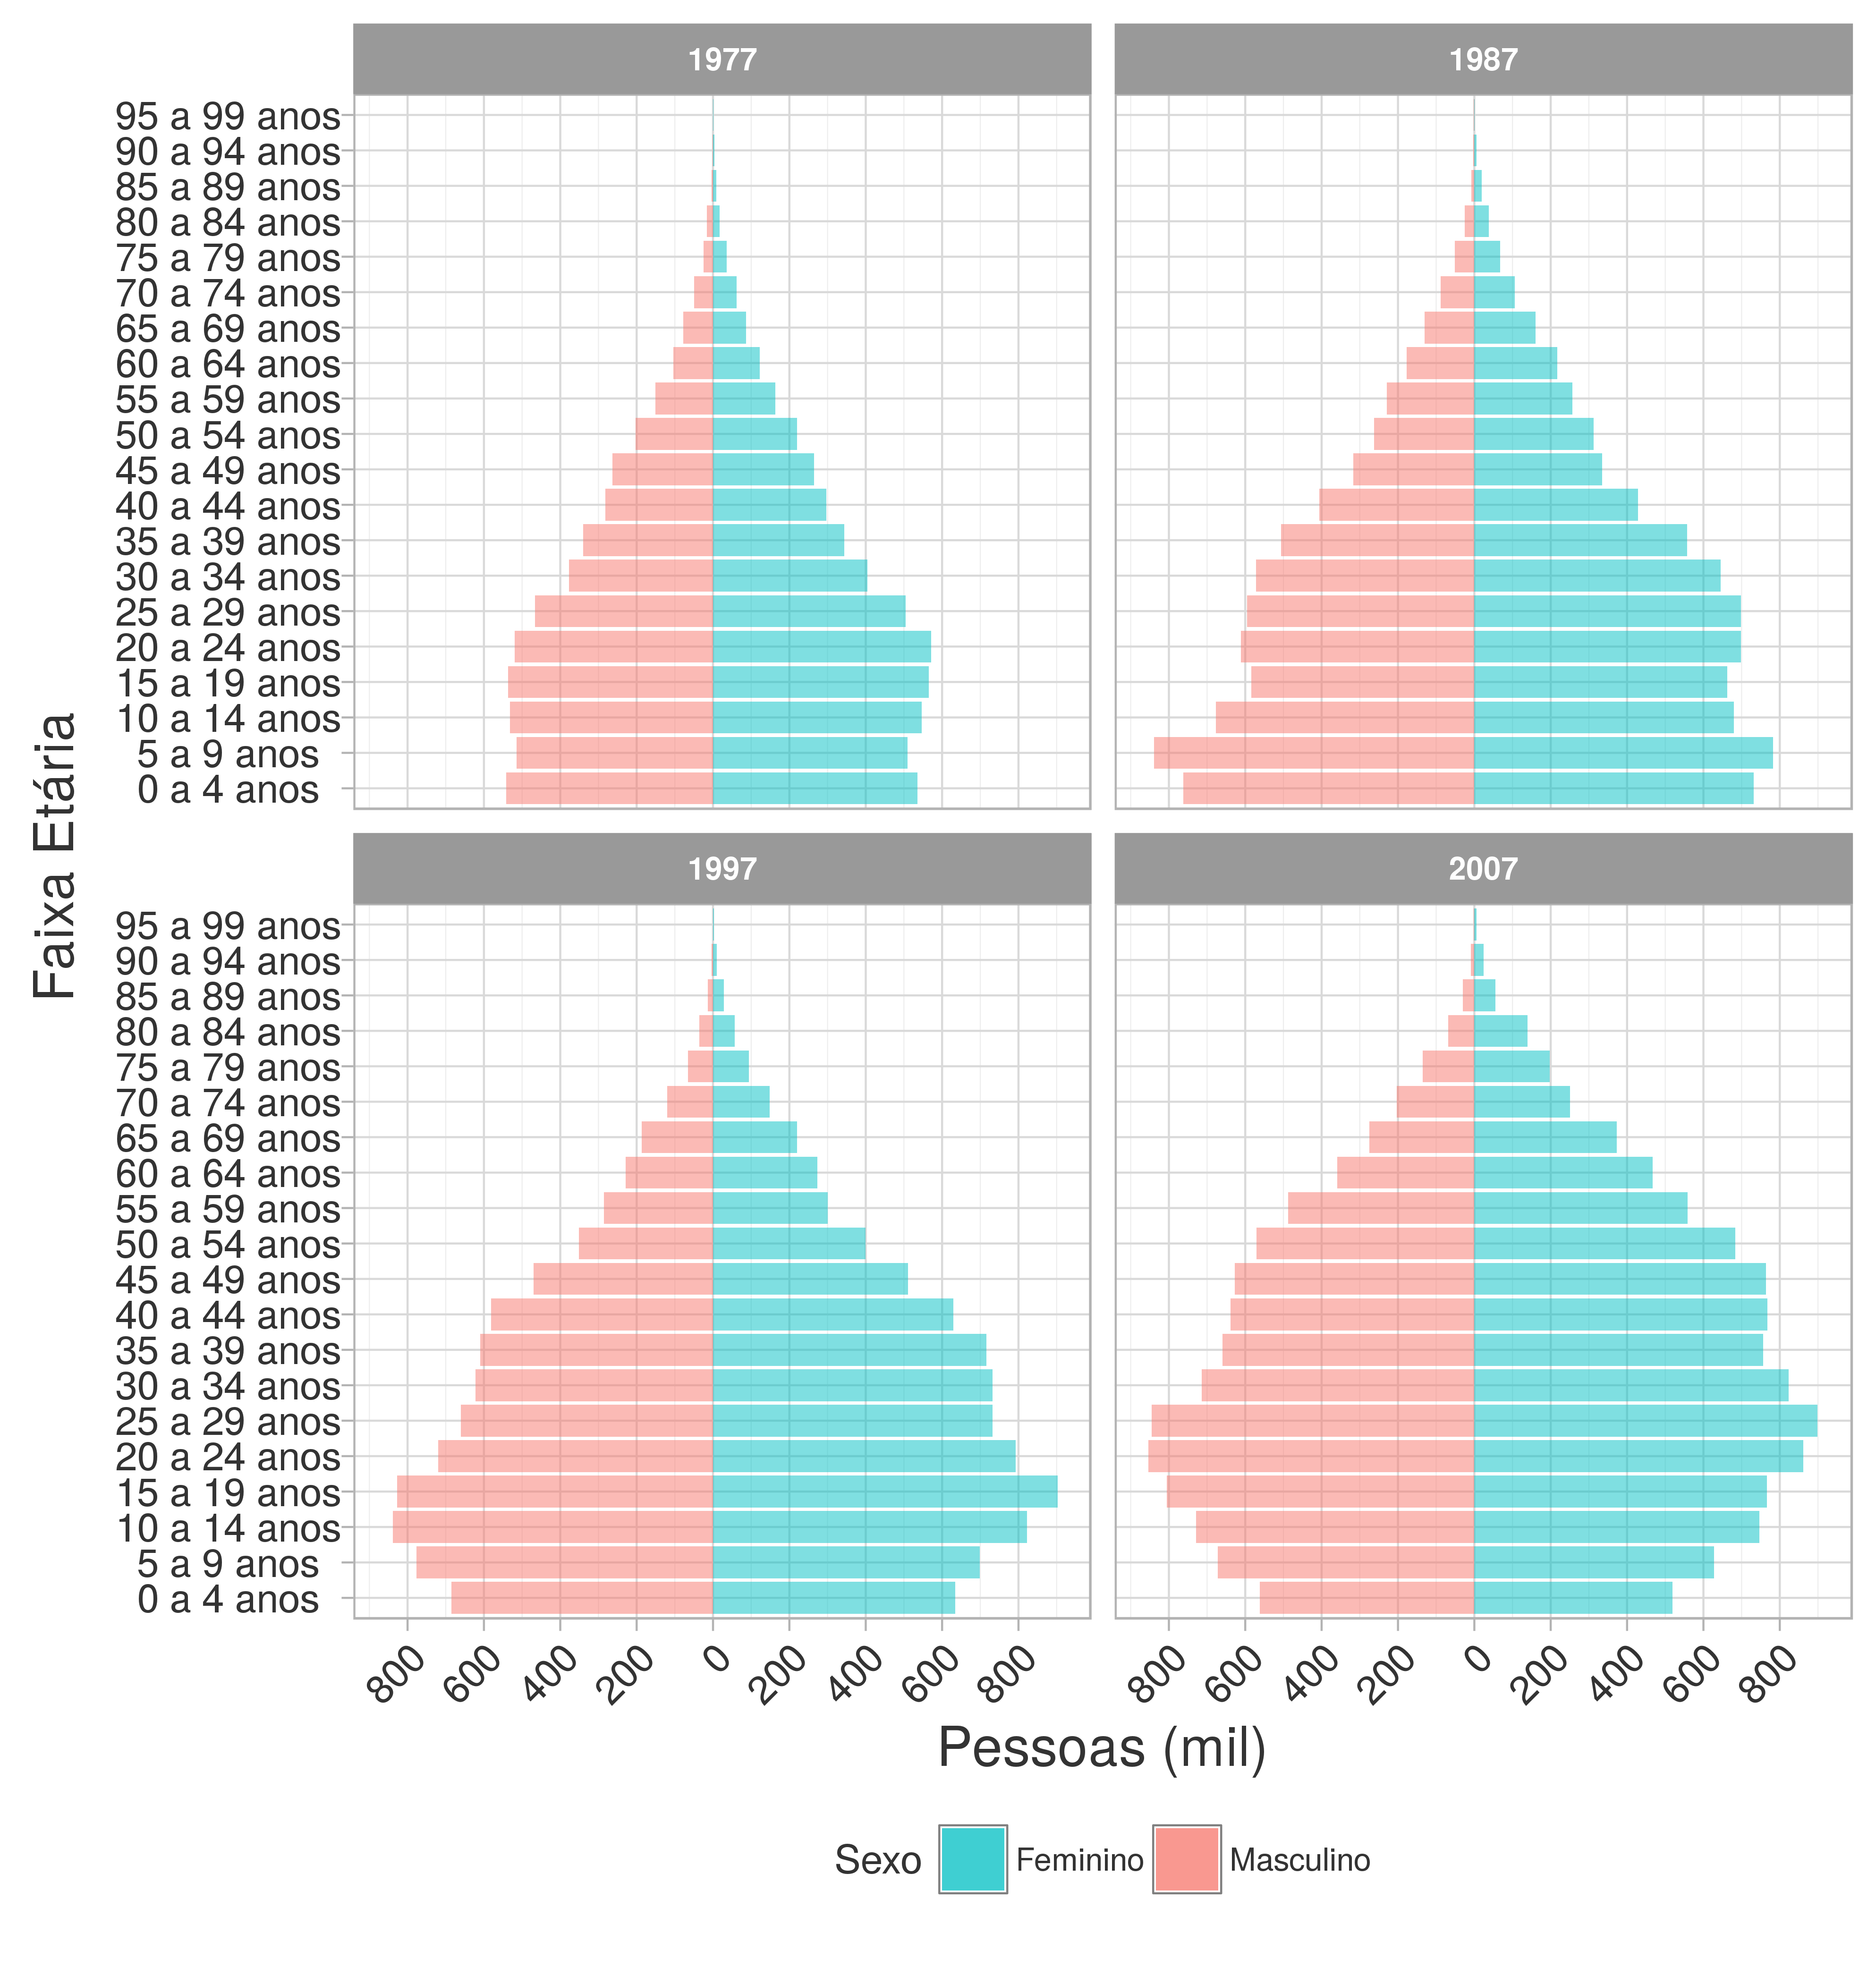
\includegraphics[width=1\textwidth]{./imagens/idade.png}%
    \end{center}%
%    \fonte{Compilação própria}
\end{grafico}%

Embora não exista relação identitária entre sexo e gênero, conforme já exposto na revisão de literatura, a variável \textbf{SEXO} é uma componente importante para compreender a categoria de análise gênero. Percebe-se na Tabela \ref{tab:prop-sexo} que em todos os anos a proporção de mulheres entrevistadas é superior à de homens, provavelmente devido ao fato de a pesquisa ser domiciliar e ser mais provável encontrar mulheres do que homens em casa.

\begin{table}[htb]
    \IBGEtab{%\renewcommand{\arraystretch}{1.5}%%\ABNTEXfontereduzida%
        \renewcommand{\arraystretch}{1.5}
        \caption{Frequências absoluta e relativa da variável SEXO, por ano}
        \label{tab:prop-sexo}
    }{%

    \begin{tabular}{ccccc}
        \toprule
        \textbf{ANO} & \textbf{1977} & \textbf{1987} & \textbf{1997} & \textbf{2007}\\ \midrule \midrule
        \textbf{\ quantidade de pessoas do sexo masculino na amostra} & 52.162 & 53.176 & 47.326 & 42.289 \\ \midrule
        \textbf{\% de pessoas do sexo masculino} & 48,3 & 48,0 & 47,9 & 46,3  \\ \midrule
%        \textbf{\% de pessoas do sexo masculino expandido} & 48,7 & 48,0 & 48,1 & 47,3  \\ \midrule        
        \textbf{\ quantidade de pessoas do sexo feminino na amostra} & 55.866 & 57.637 & 51.454 & 49.116  \\ \midrule
        \textbf{\% de pessoas do sexo feminino}  & 51,7 & 52,0 & 52,1 & 53,7  \\ \bottomrule
%        \textbf{\% de pessoas do sexo feminino expandido}  & 51,3 & 52,0 & 51,9 & 52,7 \\ \bottomrule
        \end{tabular}
    }

\end{table}
% Estatísticas para registros com F_PESS==1

Observando a variável situação familiar (\textbf{SIT_FAM}), nota-se que para as mulheres houve uma mudança ao longo dessas três décadas - ver Gráfico \ref{graf:distr-sit-fam}. Em 1977, era mais frequente elas ocuparem a posição de filhas (41,8\%), em seguida de cônjuges (36,3\%). A posição de ``pessoa responsável'' pela família é a quarta categoria mais frequente (6,3\%), de seis. Tal distribuição permanece semelhante em 1987. Em 1997, no entanto, a posição de ``pessoa responsável'' pela família (11,1\%) já quase se equipara à posição de ``outro parente/agregado(a)'' (11,3\%). Em 2007, se aproxima de um quarto proporção das mulheres entrevistadas que são responsáveis por suas famílias (22,6\%), representando aumento demais de 3,5 vezes em relação aos percentuais de 1977. O percentual de mulheres cônjuges/companheiras pouco se altera ao longo do tempo, permanecendo na faixa dos 35\%. Há diminuição da posição de empregado(a) doméstico(a) para as mulheres (da ordem da metade). Existe, também, queda da frequência daqueles que se declaram na posição de filho(a) ou enteado(a) tanto para homens como para mulheres - em ordem de grandeza próxima: cerca de 10\% para mulheres e 9\% para homens. Isso pode ser reflexo da diminuição das taxas de fecundidade%
\footnote{Por ``taxa de fecundidade total'' entende-se o número médio de filhos que teria uma mulher de uma coorte hipotética (15 e 49 anos de idade) ao final de seu período reprodutivo. Fonte: IBGE. Disponível em: \url{http://www.ibge.gov.br/home/estatistica/populacao/condicaodevida/indicadoresminimos/conceitos.shtm\#tf}} 
da população (ver Tabela \ref{tab:taxa-fecund}). Entre os homens percebe-se que houve crescimento entre aqueles com posição de ``pessoas responsável'' de cerca de 3,5\%, e também dos que declaram-se cônjuge/companheiro (cerca de 20 vezes) - esta última constatação é coerente com o fato de mais mulheres serem a principal fonte de renda doméstica, ou seja, a ``pessoa responsável'' da família.

\begin{table}[htb]
    \IBGEtab{%\renewcommand{\arraystretch}{1.5}%%\ABNTEXfontereduzida%
	    \renewcommand{\arraystretch}{1.5}
        \caption{Evolução das taxas de fecundidade no Brasil, de 1970 a 2010}
		\label{tab:taxa-fecund}
    }{%
	    \begin{tabular}{P{5.00cm} P{1.50cm} P{1.50cm} P{1.50cm} P{1.50cm} P{1.50cm}}
            \toprule
	           \headerTabCenterCell{Ano} &
   	           \headerTabCenterCell{1970} &
   	           \headerTabCenterCell{1980} &
   	           \headerTabCenterCell{1991} &
   	           \headerTabCenterCell{2000} &
   	           \headerTabCenterCell{2010} \\
		    \midrule \midrule
				Taxa de fecundidade (Brasil)&
				5,8&
				4,4&
				2,7&
				2,4&
		        1,9\\
			\midrule
				Taxa de fecundidade (Sudeste)&
				4,6&
				3,2&
				2,4&
				2,1&
		        1,7\\
			\midrule
				Taxa de fecundidade (São Paulo)&
				3,94&
				3,24&
				2,28&
				2,05&
		        1,67\\
			\bottomrule	
		\end{tabular}
    }{%
		\fonte{Compilação a partir de dados dos censos do IBGE disponíveis em \url{http://seculoxx.ibge.gov.br/populacionais-sociais-politicas-e-culturais/busca-por-palavra-chave/populacao/810-fecundidade} Acesso em 17 de novembro de 2014}
		\nota{Ao analisar as taxas de fecundidades para as Grandes Regiões, nota-se que o Sudeste tem os menores percentuais de mulheres que tiveram filhos em todos os subgrupos etários.}
		}
\end{table}

Tem-se como uma das hipótese deste trabalho que houve evolução dos padrões de mobilidade por gênero.
Articular as variáveis sexo e situação familiar é uma melhor estratégia para tentar utilizar o gênero como categoria de análise.
Assim, a transformação dos papeis sociais desempenhados por homens e mulheres dentro do núcleo familiar ao longo das últimas décadas pode ter alterado de maneira significativa os respectivos padrões de mobilidade.

\begin{grafico}[htb]%
    \caption{\label{graf:distr-sit-fam}Distribuição da variável ``SIT_FAM'', por ano e por sexo}%
    \begin{center}%
        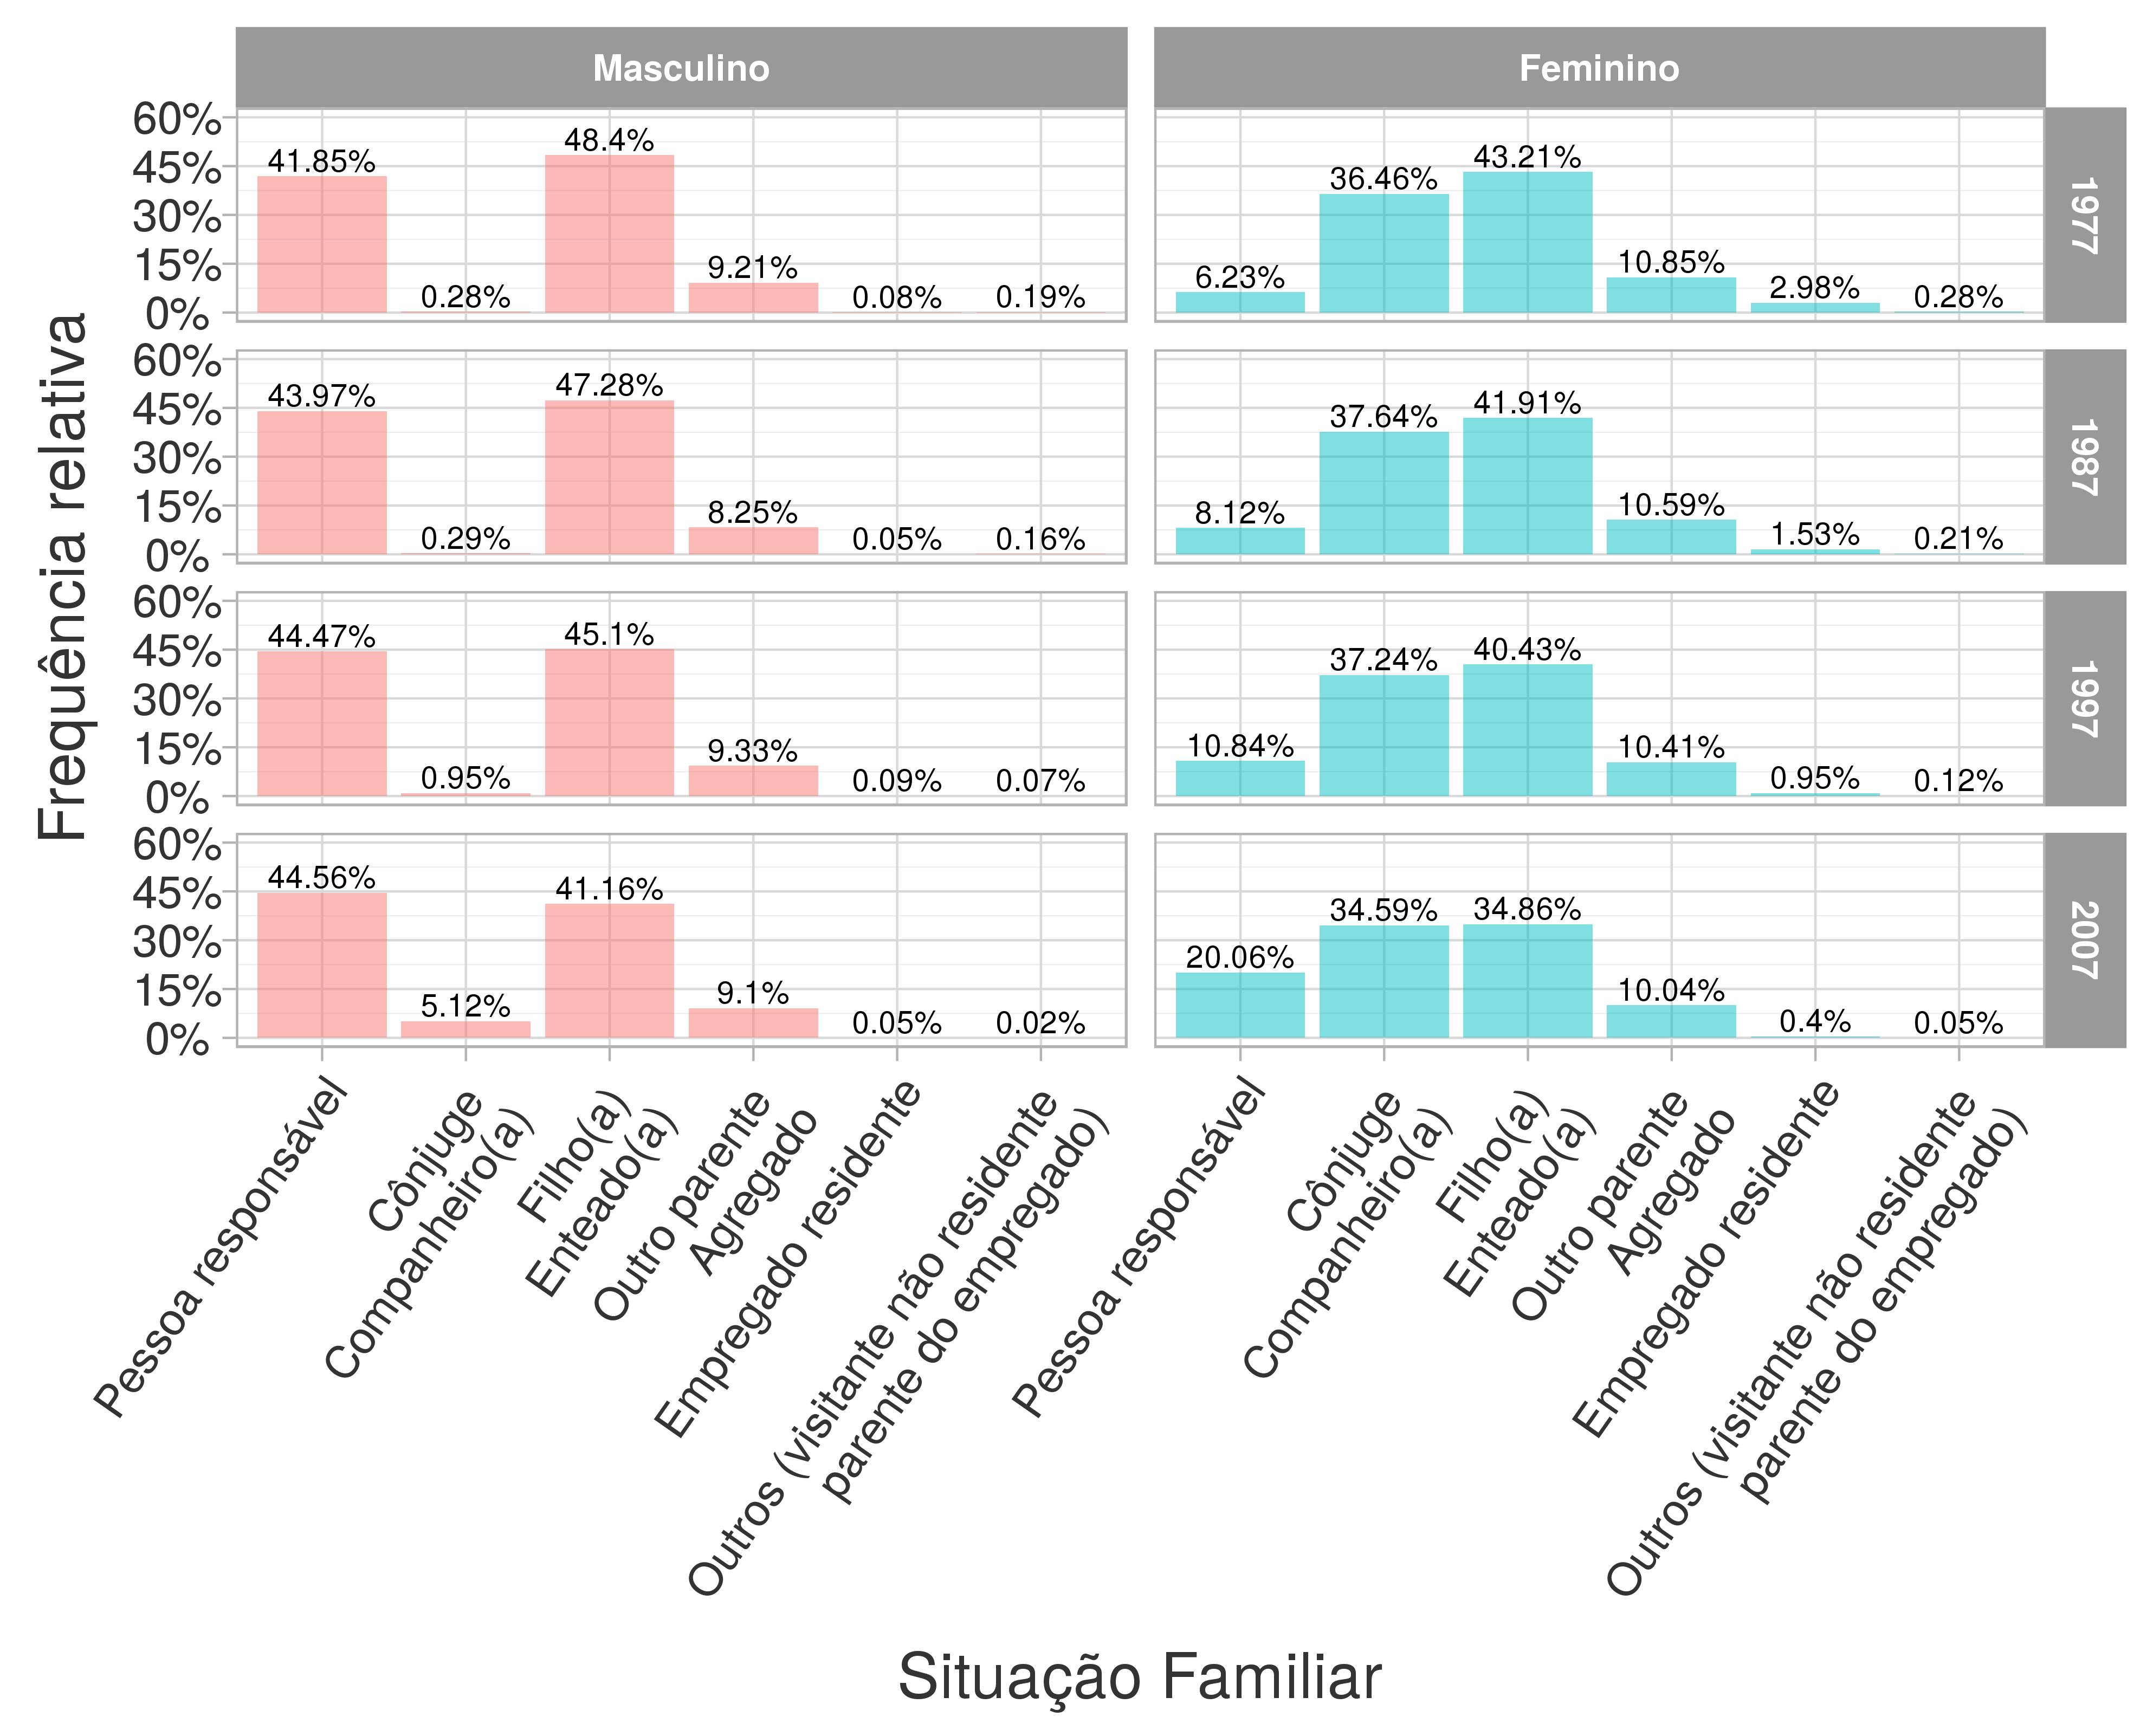
\includegraphics[width=1\textwidth]{./imagens/sit-fam.png}%
    \end{center}%
%    \fonte{Compilação própria}
\end{grafico}%

\citeauthoronline{BILT1997} (\citeyear{BILT1997}), a partir da análise de trabalhos de diversos autores, para compreender melhor o comportamento das pessoas em relação à participação em atividades e a consequente geração de viagens, 
elenca como conceito importante, além do estágio no ciclo de vida familiar e dos papéis sociais, o estilo de vida.
Duas das variáveis que auxiliam a caracterizar o estilo de vida da pessoa respondente é saber se ela estuda e se ela trabalha.

A variável \textbf{TRABALHA} foi construída a partir da variável OCUP da seguinte maneira: se a categoria da ocupação fosse 1, correspondente a ``tem trabalho'', a variável recebia valor 1, caso contrário, recebia valor 0.
A variável \textbf{ESTUDA} conta com as categorias sim (1) e não (0). Em 1987, 1997 e 2007 esta variável existe, mas somente com a categoria ``não'' em comum. Assim, as demais alternativas de resposta tornaram-se simplesmente ``sim'', independente das subdivisões que apresentassem. Para 1977, ano em que essa variável não existe, ela foi preenchida segundo o seguinte critério: a pessoa foi considerada estudante se o campo ``Zona da escola'' dela não fosse vazio ou igual a zero. Preferiu-se não utilizar a categoria ``estudante'' da variável ocupação para não perder a informação de quem estuda e trabalha, pois neste caso, estudante não seria a ocupação principal da pessoa e sim ``tem trabalho''.

% Fazendo o seguinte:
% od %>% filter(SERV_PAS_DEST==1, ZONA_DEST==ZONA_ESC, SUBZONA_DEST==SUBZONA_ESC, ANO==1) %>% select(ESTUDA, ID_PESS) %>% count(ID_PESS)
% Obtive: 72 pessoas que podem ter sido registrados erroneamnte domo estudantes em 1977

As Tabelas \ref{tab:prop-estuda} e \ref{tab:prop-trabalha} indicam as frequências das \textit{dummies} TRABALHA e ESTUDA, por ano e por sexo, em relação à população (aplicados os fatores de expansão).
Percebe-se que o percentual de trabalhadores(as) aumenta na população devido à maior participação feminina no mercado de trabalho, dado que os percentuais dos trabalhadores permanecem no mesmo patamar (24\% da população). Segmentando por sexo, vê-se que houve um aumento de quase 20\% na participação feminina no mercado de trabalho e pouco mais de 2\% de incremento na masculina.
Analisando as proporções de mulheres e homens estudantes, nota-que que houve pequeno crescimento entre 1977 e 1997 (3,2\% feminino e 2,5\% masculino) seguido de leve queda (1,5\% pra ambos sexos). A expectativa era de ter havido um grande crescimento percentual do número de estudantes, especialmente mulheres, para o período observado. O crescimento tímido pode dever-se ao fato de que, embora a população da RMSP tenha elevado seus níveis de escolarização, o crescimento (desacelerando) e o envelhecimento (em ascensão) da população implicam haver mais gente fora da faixa etária escolar do que dentro dela. As quedas no percentual de estudantes pode estar relacionada tanto ao envelhecimento da população quanto à saturação do sistema de ensino, cuja obrigatoriedade de oferta pública limita-se à Educação Básica (9 anos de Ensino Fundamental e 3 anos de Ensino Médio). 


\begin{table}[htb]
    \IBGEtab{%\renewcommand{\arraystretch}{1.5}%%\ABNTEXfontereduzida%
        \renewcommand{\arraystretch}{1.5}
        \caption{Frequências da variável TRABALHA, por ano e sexo}
        \label{tab:prop-trabalha}
    }{%

    \begin{tabular}{ccccc}
        \toprule
        \textbf{ANO} & \textbf{1977} & \textbf{1987} & \textbf{1997} & \textbf{2007}\\ \midrule \midrule
        \textbf{\% de trabalhadoras relativo ao total da população} & 9,78 & 12,18 & 16,27 & 19,88  \\ \midrule
        \textbf{\% de trabalhadores relativo ao total da população} & 24,42 & 24,73 & 24,61 & 24,82  \\ \midrule
        \textbf{\% de trabalhadoras relativo ao total de mulheres} & 19,08 & 23,44 & 31,38 & 37,76  \\ \midrule
        \textbf{\% de trabalhadores relativo ao total de homens} & 50,12 & 51,50 & 51,13 & 52,42  \\ \midrule
        \textbf{\% de trabalhadores(as) relativo ao total da população} & 34,20 & 36,91 & 40,89 & 44,70  \\ \bottomrule
        \end{tabular}
    }

\end{table}
% Estatísticas para registros com F_PESS==1

%No campo OCUP (35) as classificações de cada ano são bastante diferentes. Assim, decidiu-se por discriminar quem não respondeu, quem é estudante, quem é dono(a) de casa, que é aposentado(a), quem não tem ocupação (como por exemplo, crianças), quem está desempregado(a), quem está em licença e quem trabalha (em todas opções possíveis dadas em todas as Pesquisas OD).
%
%\begin{table}[htb]
%    \IBGEtab{%\renewcommand{\arraystretch}{1.5}%%\ABNTEXfontereduzida%
%        \renewcommand{\arraystretch}{1.5}
%        \caption{Estatísticas da variável ``OCUP''}
%        \label{tab:estat-ocup}
%    }{%
%
%    \begin{tabular}{cccccc}
%        \toprule
%        \textbf{ANO} & \textbf{1977} & \textbf{1987} & \textbf{1997} & \textbf{2007} & \textbf{Total}\\ \midrule \midrule
%        \textbf{OCUP=1}  &  3.666 & 41.082 & 41.474 & 43.838 & 163.060 \\ \hline
%        \textbf{OCUP=2}  &    736 &    668 &    447 &    574 &   2.425 \\ \hline
%        \textbf{OCUP=3}  &  3.869 &  6.664 &  7.553 & 13.125 &  31.211 \\ \hline
%        \textbf{OCUP=4}  &  2.256 &  3.304 &  6.297 &  6.500 &  18.357 \\ \hline
%        \textbf{OCUP=5}  & 16.519 & 17.118 &  8.604 &  6.717 &  48.958 \\ \hline
%        \textbf{OCUP=6}  & 22.571 & 20.283 & 11.484 &  7.082 &  61.420 \\ \hline
%        \textbf{OCUP=7}  & 20.415 & 21.409 & 22.921 & 13.569 &  78.314 \\ \hline
%        \textbf{OCUP=NA} &  4.996 &    285 &      0 &      0 &   5.281 \\ \bottomrule
%        \end{tabular}
%    }
%
%\end{table}
%% Estatísticas para registros com F_PESS==1
%
%No campo SETOR_ATIV (36), nos anos em que há opção de indicar o setor de mais de um trabalho (caso a pessoa tenha mais de um trabalho), foi considerado o setor do primeiro trabalho.
%
%\begin{table}[htb]
%    \IBGEtab{%\renewcommand{\arraystretch}{1.5}%%\ABNTEXfontereduzida%
%        \renewcommand{\arraystretch}{1.5}
%        \caption{Estatísticas da variável ``SETOR_ATIV''}
%        \label{tab:estat-setor-ativ}
%    }{%
%
%    \begin{tabular}{cccccc}
%        \toprule
%        \textbf{ANO} & \textbf{1977} & \textbf{1987} & \textbf{1997} & \textbf{2007} & \textbf{Total}\\ \midrule \midrule
%        \textbf{SETOR_ATIV=1}  &    252 &    252 &    394 &    163 &   1.061 \\ \hline
%        \textbf{SETOR_ATIV=2}  &  1.248 &  1.012 &  2.350 &  1.483 &   6.093 \\ \hline
%        \textbf{SETOR_ATIV=3}  & 12.381 & 12.391 &  6.002 &  4.676 &  35.450 \\ \hline
%        \textbf{SETOR_ATIV=4}  &  7.992 &  7.785 &  9.389 &  7.900 &  33.066 \\ \hline
%        \textbf{SETOR_ATIV=5}  &  3.336 &  3.745 &  1.693 &  1.544 &  10.318 \\ \hline
%        \textbf{SETOR_ATIV=6}  &    952 &  1.069 &  2.023 &  1.534 &   5.578 \\ \hline
%        \textbf{SETOR_ATIV=7}  & 13.618 & 16.948 & 10.522 & 15.353 &  56.441 \\ \hline
%        \textbf{SETOR_ATIV=8}  &    165 &    158 &  9.385 &      0 &   9.708 \\ \hline
%        \textbf{SETOR_ATIV=9}  & 63.086 & 67.171 & 57.022 & 12.130 & 199.409 \\ \hline
%        \textbf{SETOR_ATIV=NA} &  4.998 &    282 &      0 & 46.622 &  51.902 \\ \bottomrule
%        \end{tabular}
%    }
%
%\end{table}
%% Estatísticas para registros com F_PESS==1

\begin{table}[htb]
    \IBGEtab{%\renewcommand{\arraystretch}{1.5}%%\ABNTEXfontereduzida%
        \renewcommand{\arraystretch}{1.5}
        \caption{Frequências da variável ESTUDA, por ano e sexo}
        \label{tab:prop-estuda}
    }{%

    \begin{tabular}{ccccc}
        \toprule
        \textbf{ANO} & \textbf{1977} & \textbf{1987} & \textbf{1997} & \textbf{2007}\\ \midrule \midrule
        \textbf{\% de estudantes mulheres relativo ao total da população} & 11,94 & 12,88 & 15,17 & 13,75  \\ \midrule
        \textbf{\% de estudantes homens relativo ao total da população} & 12,55 & 12,92 & 14,99 & 13,42  \\ \midrule
        \textbf{\% de estudantes mulheres relativo ao total de mulheres} & 23,30 & 24,79 & 29,25 & 26,12  \\ \midrule
        \textbf{\% de estudantes homens relativo ao total de homens} & 25,74 & 26,90 & 31,15 & 28,35  \\ \midrule
        \textbf{\% de estudantes relativo ao total da população} & 24,49 & 25,80 & 30,17 & 27,18  \\ \bottomrule
        \end{tabular}
    }

\end{table}
% Estatísticas para registros com F_PESS==1

\newpage
No Gráfico \ref{graf:distr-grau-instr} nota-se que em 1977 tanto homens como mulheres dispunham de pouco tempo de escolaridade - cerca de três quartos da população ou era analfabeta ou possuía no máximo o fundamental incompleto. Nessa época, nos três níveis de instrução superiores a esse os homens tinham índices maiores que as mulheres. O grau de instrução (\textbf{GRAU_INSTR}) da população vai aumentando e em 1987, o grau de escolarização feminino é levemente superior ao masculino nas categorias ``fundamental completo / médio incompleto'' e ``médio completo / superior incompleto''. Na categoria ``superior completo'' o grau de instrução masculino é um pouco superior, situação que se inverte em 2007. Neste último ano de análise, as mulheres apresentam maiores percentuais nos dois níveis de maior grau de instrução e os homens, nos dois níveis de menor grau de instrução.

%Mesmo assim, as marcas para ambos são bastante semelhantes e indicam esforços de políticas públicas no sentido de universalizar os Ensinos Fundamental e Médio no Brasil \ref{tab:grau-instr-ef-em}.
%
%\begin{table}[htb]
%    \IBGEtab{%\renewcommand{\arraystretch}{1.5}%%\ABNTEXfontereduzida%
%	    \renewcommand{\arraystretch}{1.5}
%        \caption{Crescimento de matrículas no Ensino Fundamental e Ensino Médio, no Brasil, entre 1975 e 2005}
%		\label{tab:grau-instr-ef-em}
%    }{%
%	    \begin{tabular}{P{2.00cm} P{4.00cm} P{4.00cm}}
%            \toprule
%	           \headerTabCenterCell{Ano} &
%   	           \headerTabCenterCell{Matrículas no Ensino Fundamental} &
%   	           \headerTabCenterCell{Matrículas no Ensino Médio}\\
%		    \midrule \midrule
%				1975&
%		    	100*&
%				100*\\
%			\midrule
%				1980&
%				115,6&
%		        113,1\\
%			\midrule
%				1990&
%				141,0**&
%		        180,8\\
%			\midrule
%				1996&
%				169,5&
%		        296,4\\
%			\midrule
%				2000&
%				182,7&
%		        423,2\\
%			\midrule
%				2005&
%				171,5&
%		        466,5\\
%			\bottomrule	
%		\end{tabular}
%    }{%
%		\fonte{Adaptado de \citeauthoronline{OLIVEIRA2007} (\citeyear{OLIVEIRA2007})}
%		\nota{* Tomou-se por referência o ano de 1975 (1975=100). 
%		** O valor refere-se ao ano de 1989.}
%	}
%\end{table}

\begin{grafico}[htb]%
    \caption{\label{graf:distr-grau-instr} Distribuição da variável ``GRAU_INSTR'', por ano e por sexo}%
    \begin{center}%
        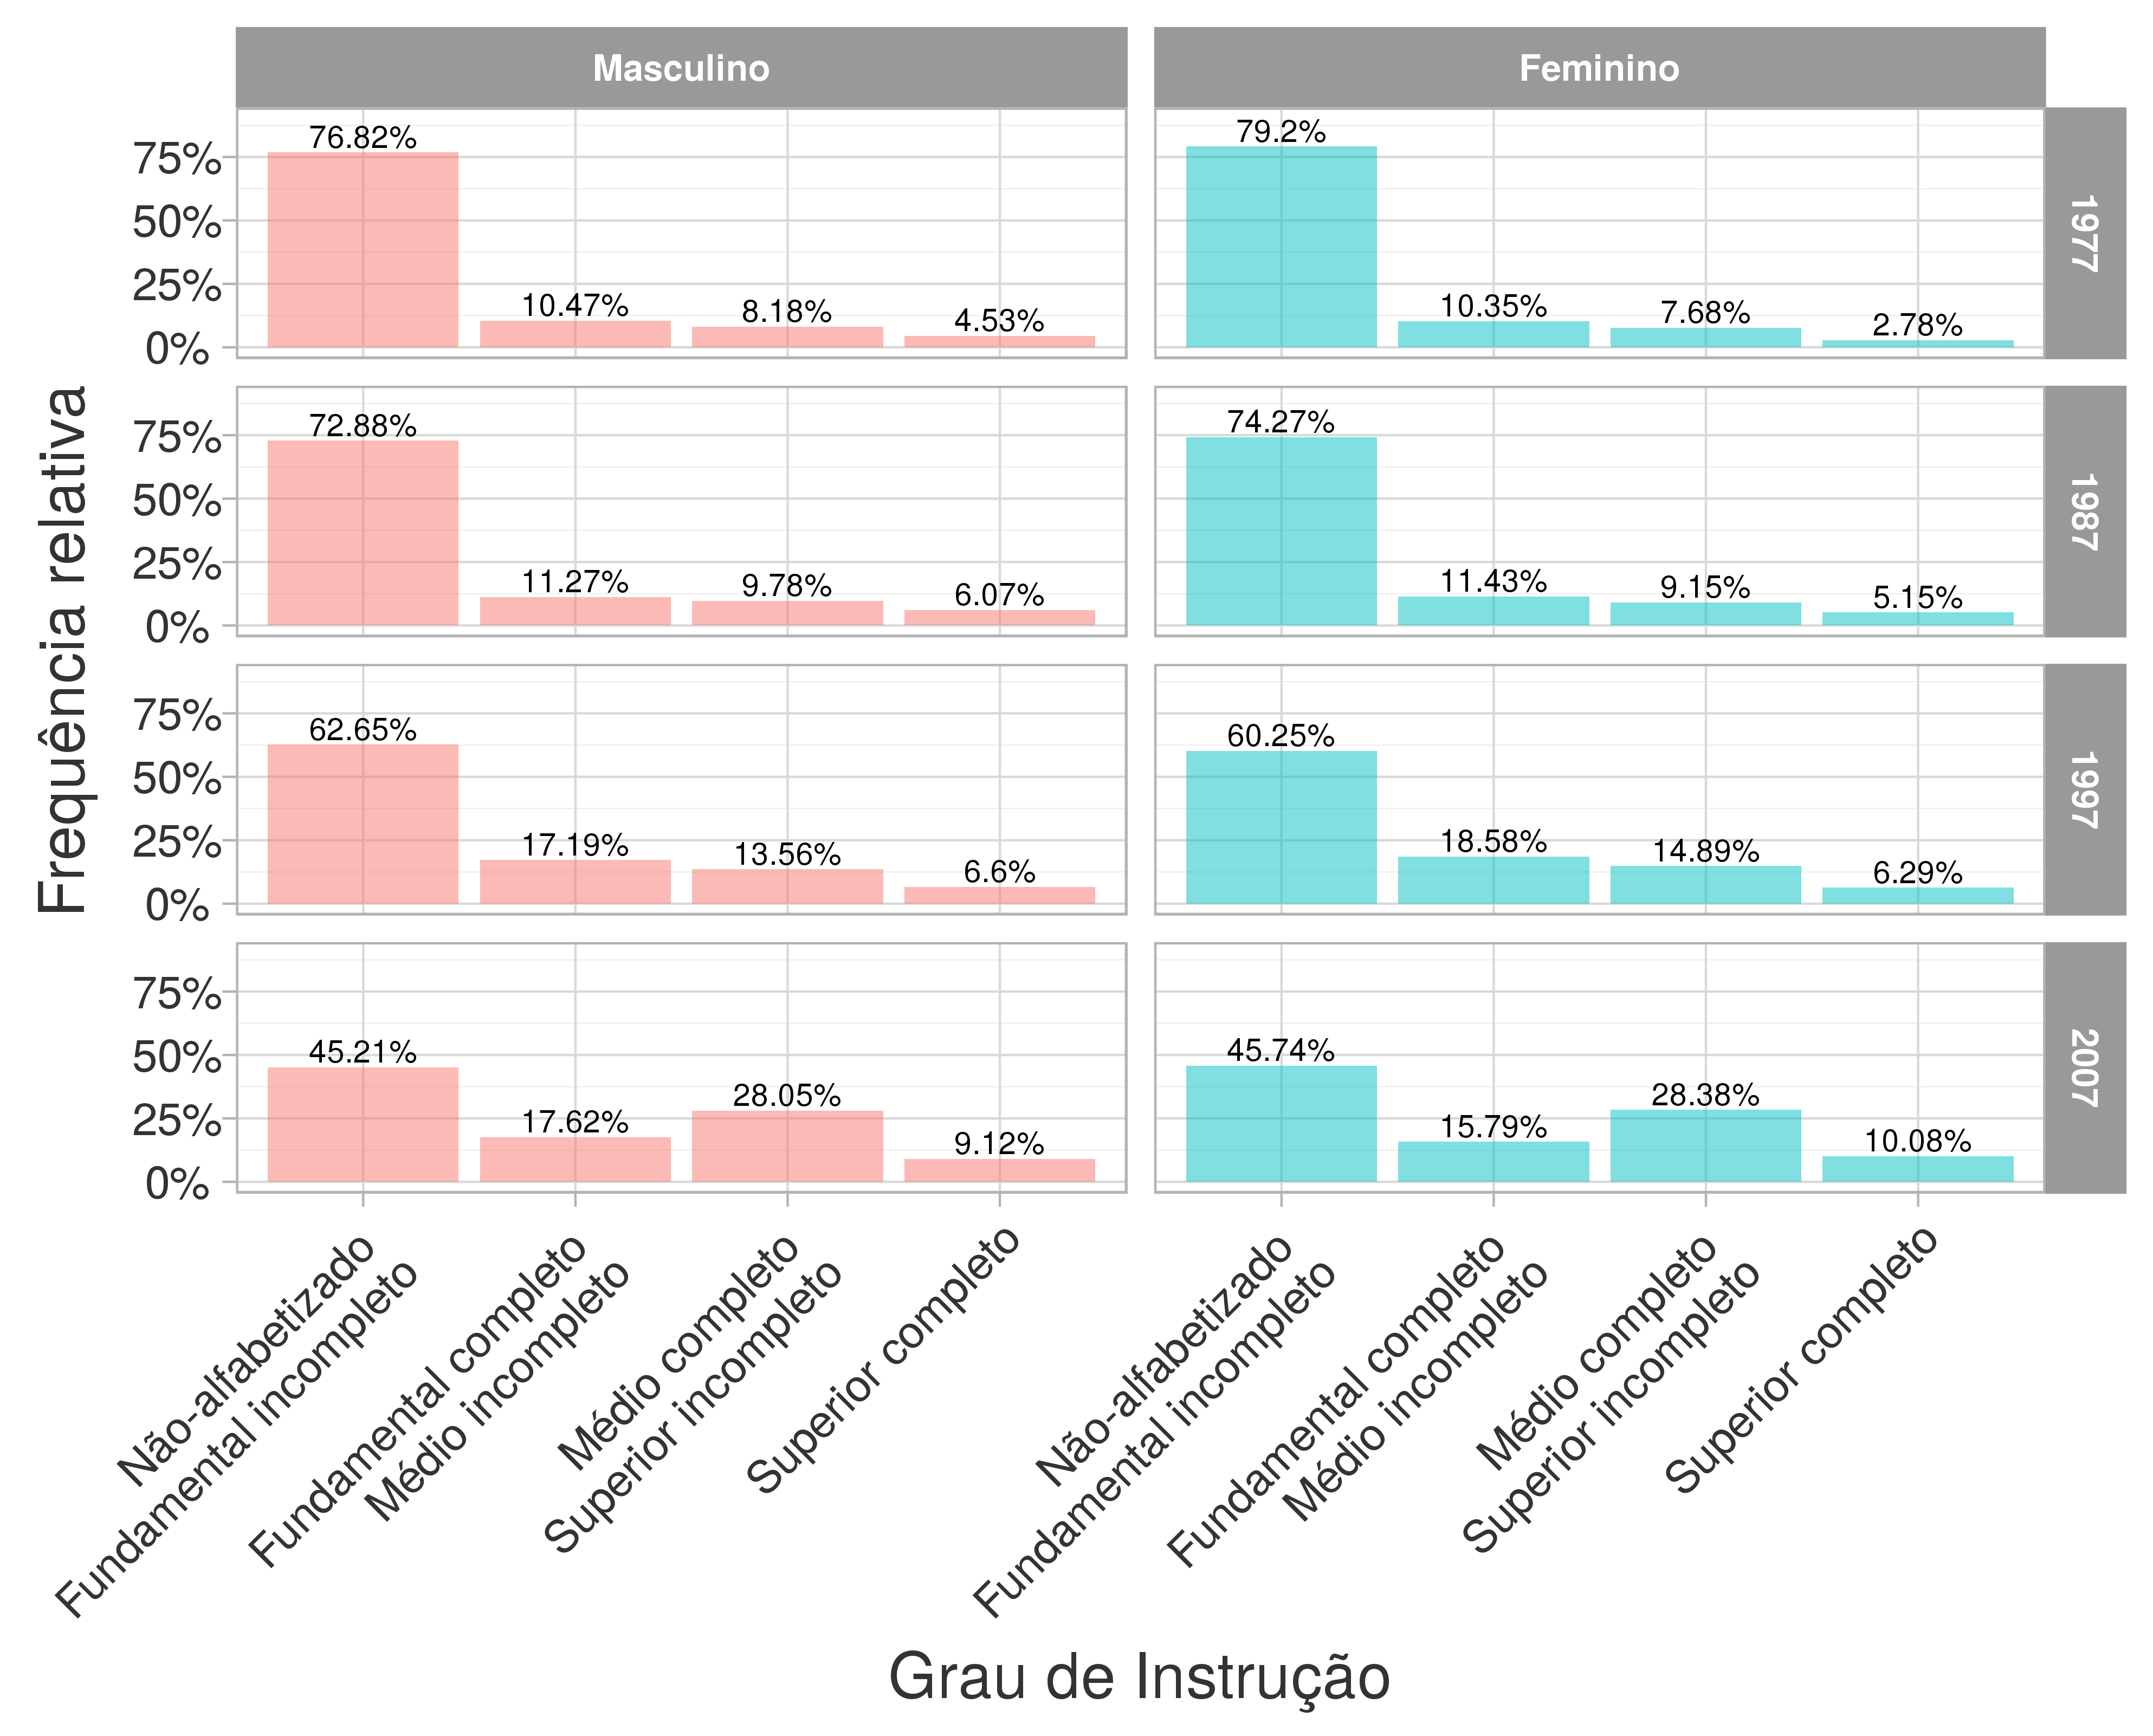
\includegraphics[width=1\textwidth]{./imagens/grau-instr.png}%
    \end{center}%
%    \fonte{Compilação própria}
\end{grafico}%

A elevação do grau de instrução entre 1977 e 2007 influencia não apenas as viagens motivo trabalho (por eventual aumento da empregabilidade) mas também as viagens motivo escola, realizadas por um contingente de pessoas cada vez maior, mais diverso e contendo mais faixas etárias.
A maior participação feminina no mercado de trabalho além de impactar as rendas (individual e familiar) deve influenciar bastante as viagens motivo trabalho. 

A renda individual (variável \textbf{REN_IND}) tem seu comportamento de médias e medianas análogo ao da renda familiar. Explora-se aqui, então, as rendas individuais de quem tem 10 anos ou mais
\footnote{Foi adotada essa idade como limite de corte porque o IBGE produz estatísticas de ``valor do rendimento nominal médio mensal e mediano mensal para pessoas de 10 anos ou mais de idade, total e com rendimento''. Fonte: \url{http://www.sidra.ibge.gov.br/bda/tabela/listabl.asp?c=1381&z=cd&o=7} Acesso em 15 de janeiro de 2016}, 
segmentando por sexo e e por duas situações familiares: pessoa responsável e cônjuge/companheiro(a).
Em todos anos, a renda individual média masculina é superior à feminina para a mesma situação familiar, conforme Tabela \ref{tab:estat-ren-ind}. 
Em 1977, quando pessoa responsável pela família, o homem ganhava 2,5 vezes mais que a mulher em mesma condição. Essa marca vem caindo (cada vez mais devagar) até que, em 2007, eles ganham 1,5 vezes mais do que elas.
Para a situação de cônjuges, a relação entre as rendas médias masculina e feminina giram em média em torno de dois, oscilando para 1,8 em 1987 e 2,4 em 1997. Ou seja, homens cônjuges em geral ganham cerco do dobro das mulheres cônjuges e essa situação pouco se alterou com o passar das décadas.

\begin{table}[htb]
\centering
   \IBGEtab{%\renewcommand{\arraystretch}{1.5}%%\ABNTEXfontereduzida%
        \renewcommand{\arraystretch}{1.5}
        \caption{Estatísticas da variável ``REN_IND''}
        \label{tab:estat-ren-ind}
    }{%

    \begin{tabular}{ccccccc}
        \toprule
        \textbf{Homem} & \multicolumn{3}{c}{\textbf{pessoa responsável}} & \multicolumn{3}{c}{\textbf{cônjuge/companheiro}} \\ \hline
        \textbf{ANO}   & \textbf{Média} & \textbf{Desvio Padrão} & \textbf{Mediana} & \textbf{Média} & \textbf{Desvio Padrão} & \textbf{Mediana} \\ \midrule \midrule
        \textbf{1977}  & 2.762,85 & 3.910,71 & 1.478,21 &   703,24 & 1.461,49 &   0,00 \\ \hline
        \textbf{1987}  & 1.610,76 & 2.146,33 &   985,80 &   522,67 &   953,85 &  99,64 \\ \hline
        \textbf{1997}  & 1.769,16 & 3.272,09 &   873,61 & 1.143,30 & 2.115,36 & 485,34 \\ \hline
        \textbf{2007}  & 1.265,37 & 2.330,39 &   600,00 & 1.147,71 & 2.396,79 & 300,00 \\ \hline                
        \textbf{Total} & 1.869,37 & 3.059,03 &   970,68 & 1.098,29 & 2.280,25 & 291,73 \\\bottomrule

        \textbf{Mulher} & \multicolumn{3}{c}{\textbf{pessoa responsável}} & \multicolumn{3}{c}{\textbf{cônjuge/companheira}} \\ \hline
        \textbf{ANO}   & \textbf{Média} & \textbf{Desvio Padrão} & \textbf{Mediana} & \textbf{Média} & \textbf{Desvio Padrão} & \textbf{Mediana} \\ \midrule \midrule
        \textbf{1977}  & 1.098,95 & 2.108,50 & 506,81 & 306,95 & 1.097,29 & 0,00 \\ \hline
        \textbf{1987}  &   807,79 & 1.398,68 & 397,99 & 284,87 &   872,94 & 0,00 \\ \hline
        \textbf{1997}  & 1.034,83 & 1.923,79 & 465,93 & 478,78 & 1.332,07 & 0,00 \\ \hline
        \textbf{2007}  &   866,43 & 1.661,52 & 380,00 & 498,39 & 1.204,76 & 0,00 \\ \hline                
        \textbf{Total} &   926,53 & 1.752,55 & 388,27 & 383,26 & 1.131,58 & 0,00 \\\bottomrule

    \end{tabular}
    
    }

\end{table}
% Estatísticas para registros com F_PESS==1, filtors em IDADE (>9), SEXO e SIT_FAM
% Não expandido com FE_PESS

\begin{grafico}[htb]%
    \caption{\label{graf:clas-econ-ren-ind}Distribuição da variável ``FAIXA_REN_IND'', por ano}%
        \begin{center}%
        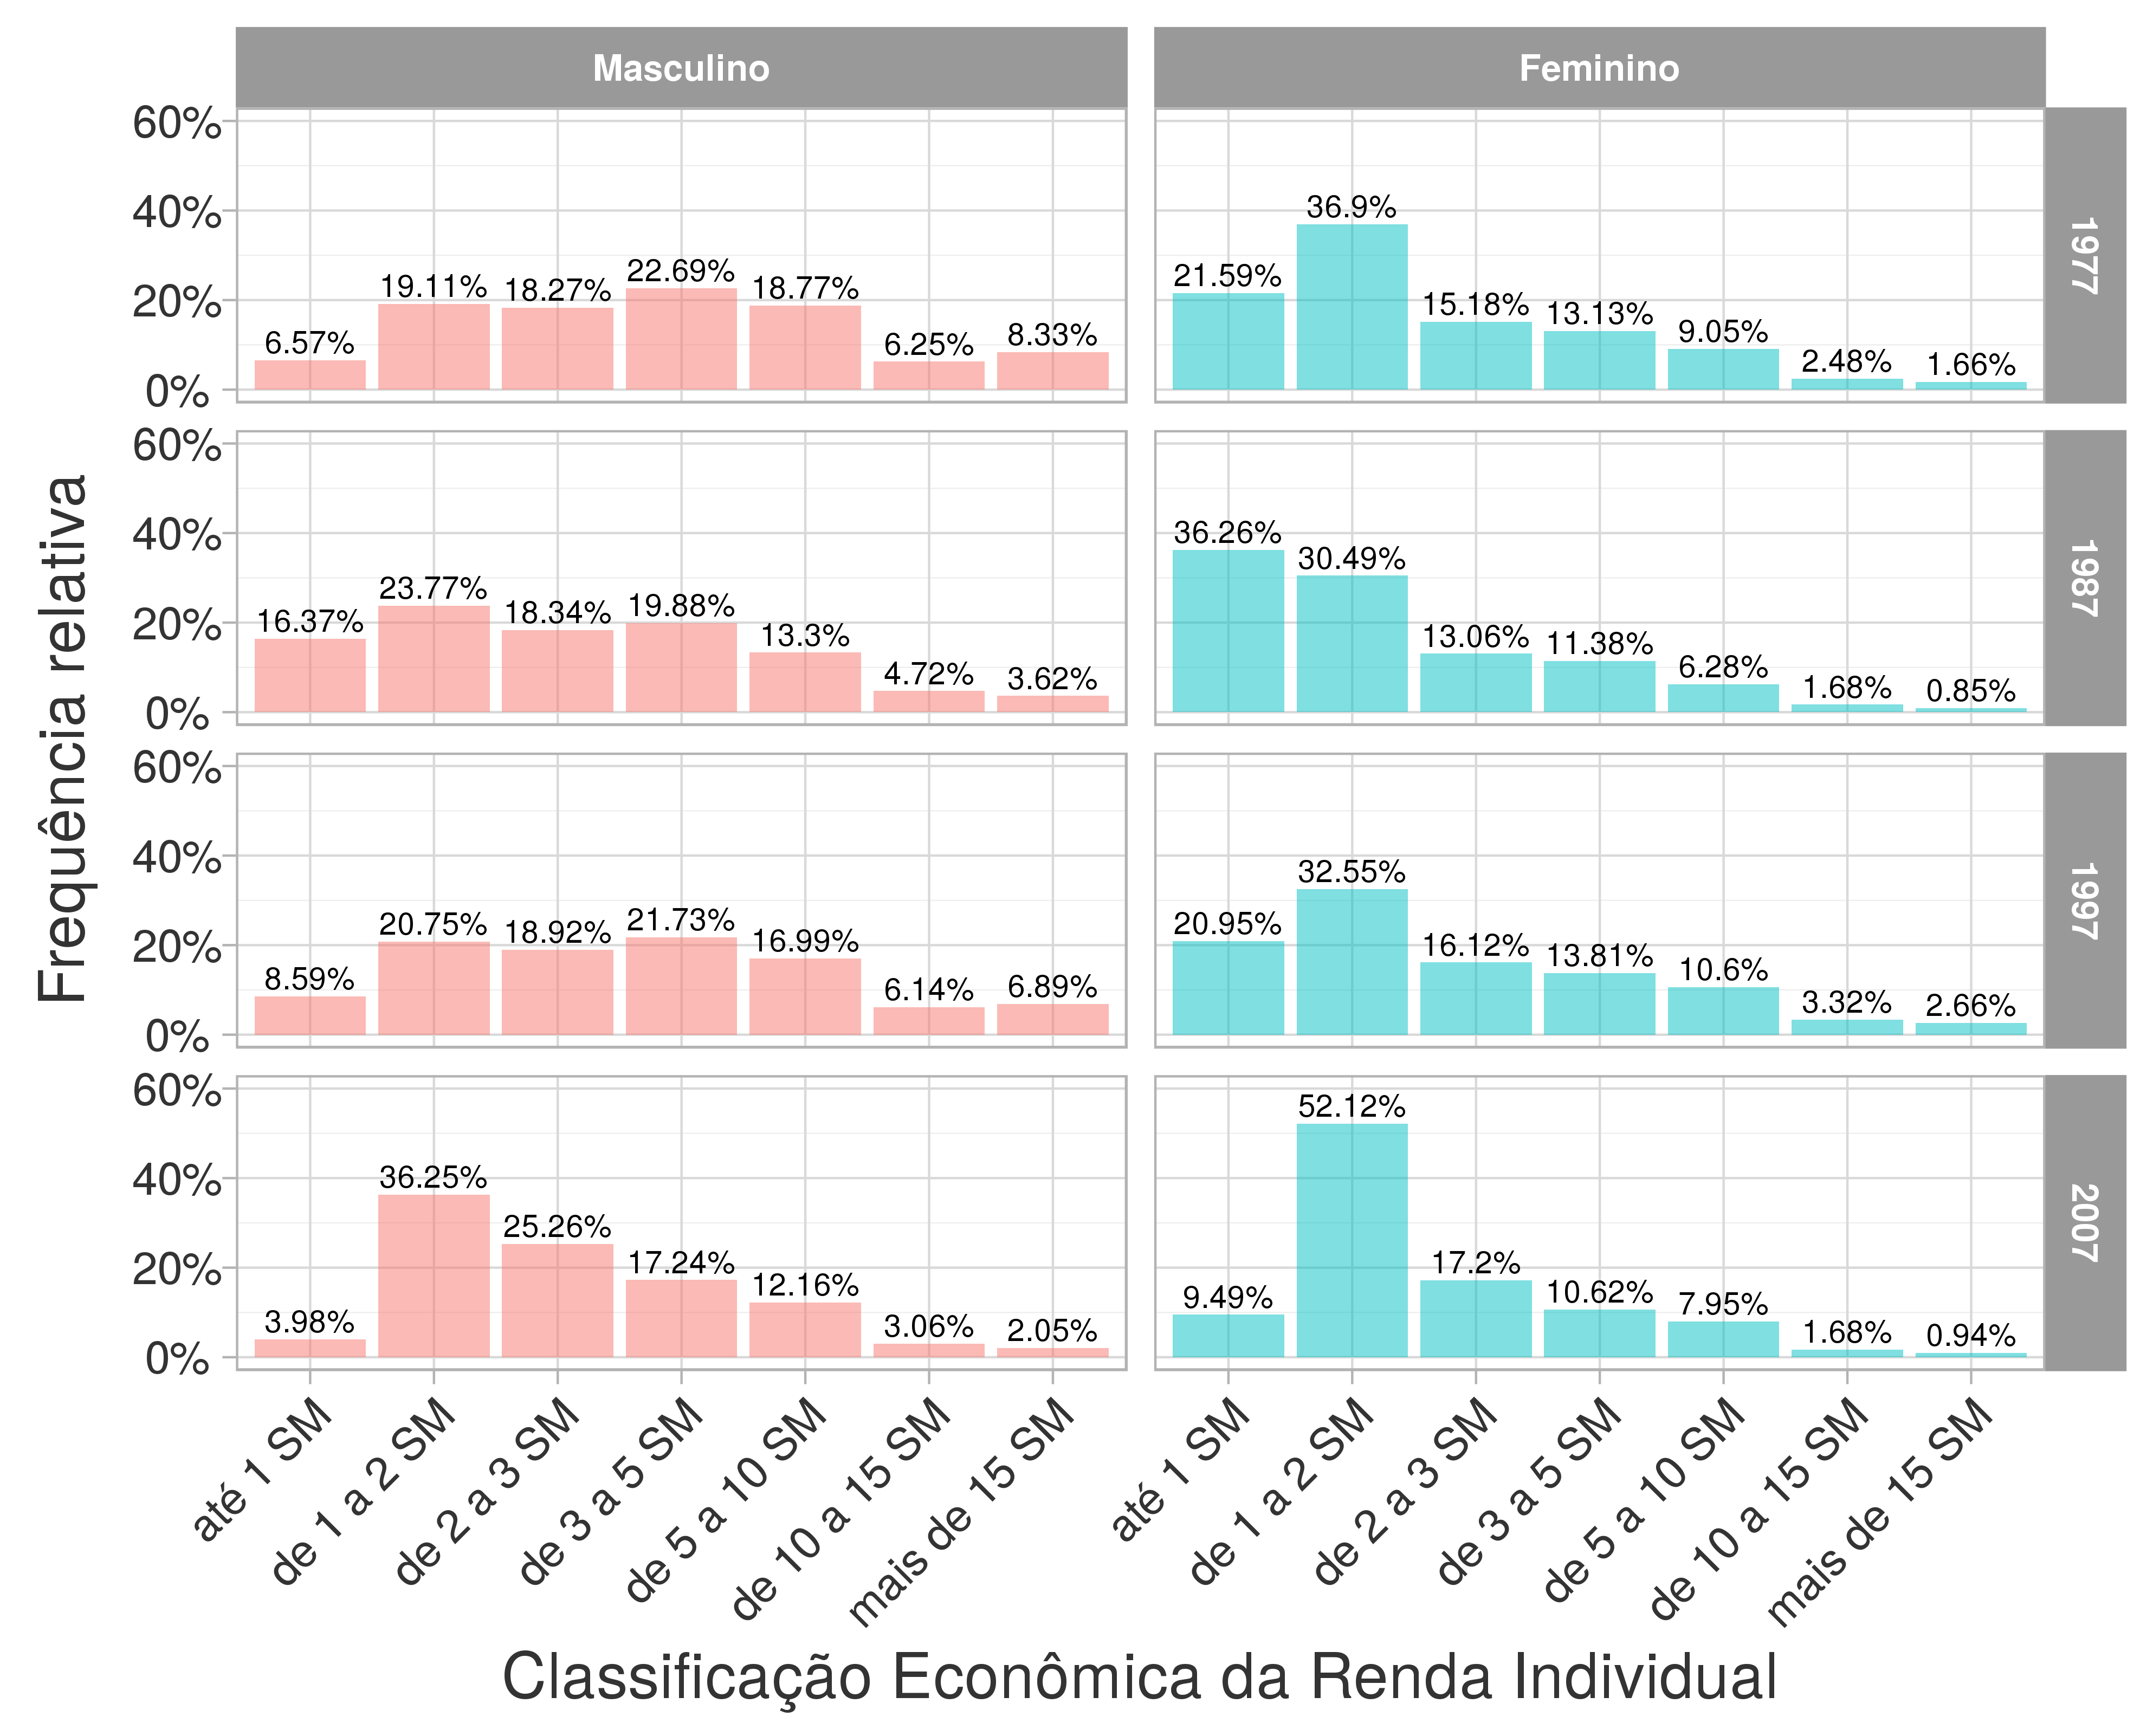
\includegraphics[width=1\textwidth]{./imagens/clas-econ-ren-ind.png}%
    \end{center}%
    %\fonte{Compilação própria}
\end{grafico}%

Pelo Gráfico \ref{graf:clas-econ-ren-ind} percebe-se que houve um aumento de quem ganhava até 1 salário mínimo entre 1977 e 1987. De 1987 para 2007 a proporção de pessoas que têm rendimentos nessa faixa salarial vem decrescendo. De 1977 a 1997 a faixa de rendimento de 1 a 2 salários mínimos ficou próxima dos 25\% e, em 2007, cresceu aproximadamente 10\%. A faixa de rendimento de 2 a 3 salários mínimos subiu cerca de 3\% entre 1977 e 2007, o mesmo que a faixa de rendimentos de 3 a 5 salários mínimos diminuiu no período.


\clearpage

\section{Análises Preliminares}\label{sec:analises-preliminares}

O grupo de análises que se segue busca compreender como é o comportamento das pessoas e das famílias em termo de viagens realizadas, em cada ano e diferencialmente entre os anos, olhando para tanto variáveis como:
\begin{compactitem}
\item número de viagens;
\item modos de viagem;
\item motivos de viagens;
\item duração das viagens;
\item distâncias das viagens.
\end{compactitem}

A variável \textbf{TOT_VIAG} representa o número total de viagens realizadas pela pessoa. Não existem \textit{missing values} neste campo, os valores mínimos para todos anos e ambos sexo são 0, bem como também são 0 os valores do primeiro quartil (25\%). Os valores das demais estatísticas (considerando os fatores de expansão para a população) estão apresentados na Tabela \ref{tab:estat-tot-viag}. Conforme já era de se esperar, para quem faz viagem no dia da pesquisa (número de viagem é não nulo) existe a predominância do valor 2, ou seja, são pessoas que saem de suas residências com um propósito único (trabalhar, estudar, fazer compras) e depois retornam à residência após a atividade.
Percebe-se que, independente do sexo, o número médio de viagens por pessoa em relação a 1977 caiu um pouco em 1987 e 1997 (de 1,67 para 1,64) e subiu novamente em 2007 (para 1,70). Os desvios padrão caíram ao longo do tempo, indicando tendência de menor dispersão dos dados. Os valores de assimetria são positivos, indicando maior concentração à esquerda e cauda longa à direita da distribuição. Os valores de curtose evidenciam não tratar-se de distribuição normal.

Analisando esses dados segmentados por sexo, vê-se que as medianas são iguais. O número médio e máximo de viagens para mulheres é sempre inferior ao dos homens, para o mesmo ano. Os valores de assimetria para o sexo feminino e o masculino são positivos e convergem para o valor geral com o passar das décadas. 
A diferença entre o número médio de viagens de mulheres e homens vem diminuindo.

\begin{table}[htb]
\centering
   \IBGEtab{%\renewcommand{\arraystretch}{1.5}%%\ABNTEXfontereduzida%
        \renewcommand{\arraystretch}{1.5}
        \caption{Estatísticas da variável ``TOT_VIAG'', por ano e por sexo}
        \label{tab:estat-tot-viag}
    }{%

    \begin{tabular}{ccccccc}
        \toprule
        \textbf{Geral} & \multicolumn{3}{c}{\textbf{}} & \multicolumn{3}{c}{\textbf{}} \\ \hline
        \textbf{ANO}   & \textbf{Média} & \textbf{Desvio Padrão} & \textbf{Mediana} & \textbf{Máximo} & \textbf{Assimetria} & \textbf{Curtose} \\ \midrule \midrule
        \textbf{1977}  & 1,67 & 1,75 & 2,00 & 24 & 1,48 & 4,71 \\ \hline
        \textbf{1987}  & 1,64 & 1,61 & 2,00 & 24 & 1,37 & 4,80 \\ \hline
        \textbf{1997}  & 1,64 & 1,60 & 2,00 & 21 & 1,36 & 4,38 \\ \hline
        \textbf{2007}  & 1,70 & 1,48 & 2,00 & 18 & 1,09 & 3,53 \\\bottomrule          

        \textbf{Sexo Feminino} & \multicolumn{3}{c}{\textbf{}} & \multicolumn{3}{c}{\textbf{}} \\ \hline
        \textbf{ANO}   & \textbf{Média} & \textbf{Desvio Padrão} & \textbf{Mediana} & \textbf{Máximo} & \textbf{Assimetria} & \textbf{Curtose} \\ \midrule \midrule
        \textbf{1977}  & 1,35 & 1,58 & 2,00 & 16 & 1,35 & 3,16 \\ \hline
        \textbf{1987}  & 1,42 & 1,58 & 2,00 & 19 & 1,40 & 4,14 \\ \hline
        \textbf{1997}  & 1,52 & 1,62 & 2,00 & 18 & 1,48 & 5,00 \\ \hline
        \textbf{2007}  & 1,61 & 1,51 & 2,00 & 17 & 1,10 & 2,88 \\\bottomrule
        
        \textbf{Sexo Masculino} & \multicolumn{3}{c}{\textbf{}} & \multicolumn{3}{c}{\textbf{}} \\ \hline
        \textbf{ANO}   & \textbf{Média} & \textbf{Desvio Padrão} & \textbf{Mediana} & \textbf{Máximo} & \textbf{Assimetria} & \textbf{Curtose} \\ \midrule \midrule
        \textbf{1977}  & 2,01 & 1,85 & 2,00 & 24 & 1,52 & 5,31 \\ \hline
        \textbf{1987}  & 1,88 & 1,61 & 2,00 & 24 & 1,41 & 5,83 \\ \hline
        \textbf{1997}  & 1,78 & 1,58 & 2,00 & 21 & 1,26 & 3,87 \\ \hline
        \textbf{2007}  & 1,81 & 1,44 & 2,00 & 18 & 1,12 & 4,48 \\\bottomrule             
       
    \end{tabular}
    }{%
%		\fonte{Elaboração própria}
	}
\end{table}
% Estatísticas para registros com F_PESS==1, filtro por SEXO
% Expandido com FE_PESS

Ao considerar apenas quem faz viagens, os valores mínimos para todos anos e ambos sexo passam para 1, bem como também são 1 os valores do primeiro quartil (25\%). Os valores das demais estatísticas (considerando os fatores de expansão para a população) estão apresentados na Tabela \ref{tab:estat-tot-viag-nao-nula}.
Para todos anos e para ambos sexos, as médias passaram para valores superiores a 2 e há uma tendência de diminuição do número de viagens por pessoa com o passar do tempo.
Os desvios padrão caíram ao longo do tempo para as mulheres e para o conjunto de homens e mulheres, indicando menor dispersão dos dados. Os valores de assimetria aumentaram e continuaram positivos, indicando maior concentração à esquerda e cauda longa à direita da distribuição. Os valores de curtose também aumentaram e a distribuição continua não sendo aderente à normalidade.
Na segmentação por sexo, as medianas e a quantidade máxima de viagens permanecem iguais.
Entretanto, o número médio de viagens para mulheres era superior ao dos homens em 1977 e 1987. Já em 1997 e em 2007, a média delas passa a ser inferior à deles.

\begin{table}[htb]
\centering
   \IBGEtab{%\renewcommand{\arraystretch}{1.5}%%\ABNTEXfontereduzida%
        \renewcommand{\arraystretch}{1.5}
        \caption{Estatísticas da variável ``TOT_VIAG'', por ano e por sexo, considerando apenas quem fez viagem}
        \label{tab:estat-tot-viag-nao-nula}
    }{%

    \begin{tabular}{ccccccc}
        \toprule
        \textbf{Geral} & \multicolumn{3}{c}{\textbf{}} & \multicolumn{3}{c}{\textbf{}} \\ \hline
        \textbf{ANO}   & \textbf{Média} & \textbf{Desvio Padrão} & \textbf{Mediana} & \textbf{Máximo} & \textbf{Assimetria} & \textbf{Curtose} \\ \midrule \midrule
        \textbf{1977}  & 2,75 & 1,44 & 2,00 & 24 & 2,70 & 11,75 \\ \hline
        \textbf{1987}  & 2,61 & 1,27 & 2,00 & 24 & 3,01 & 14,66 \\ \hline
        \textbf{1997}  & 2,58 & 1,27 & 2,00 & 21 & 2,89 & 12,59 \\ \hline
        \textbf{2007}  & 2,49 & 1,11 & 2,00 & 18 & 2,94 & 12,77 \\\bottomrule          

        \textbf{Sexo Feminino} & \multicolumn{3}{c}{\textbf{}} & \multicolumn{3}{c}{\textbf{}} \\ \hline
        \textbf{ANO}   & \textbf{Média} & \textbf{Desvio Padrão} & \textbf{Mediana} & \textbf{Máximo} & \textbf{Assimetria} & \textbf{Curtose} \\ \midrule \midrule
        \textbf{1977}  & 2,85 & 1,57 & 2,00 & 16 & 2,65 & 11,19 \\ \hline
        \textbf{1987}  & 2,61 & 1,29 & 2,00 & 19 & 3,08 & 15,47 \\ \hline
        \textbf{1997}  & 2,56 & 1,26 & 2,00 & 18 & 2,73 & 10,55 \\ \hline
        \textbf{2007}  & 2,47 & 1,09 & 2,00 & 17 & 3,10 & 15,08 \\\bottomrule
        
        \textbf{Sexo Masculino} & \multicolumn{3}{c}{\textbf{}} & \multicolumn{3}{c}{\textbf{}} \\ \hline
        \textbf{ANO}   & \textbf{Média} & \textbf{Desvio Padrão} & \textbf{Mediana} & \textbf{Máximo} & \textbf{Assimetria} & \textbf{Curtose} \\ \midrule \midrule
        \textbf{1977}  & 2,62 & 1,23 & 2,00 & 24 & 2,55 &  9,84 \\ \hline
        \textbf{1987}  & 2,60 & 1,24 & 2,00 & 24 & 2,90 & 13,40 \\ \hline
        \textbf{1997}  & 2,59 & 1,29 & 2,00 & 21 & 3,06 & 14,56 \\ \hline
        \textbf{2007}  & 2,52 & 1,13 & 2,00 & 18 & 2,79 & 10,71 \\\bottomrule             
       
    \end{tabular}
    }{%
%		\fonte{Elaboração própria}
	}
\end{table}
% Estatísticas para registros com F_PESS==1, filtro por SEXO
% Expandido com FE_PESS

Foram feitos testes t para avaliar se as médias de mulheres e de homens eram estatisticamente diferentes, em cada ano, tanto considerando quem não fez viagem (TOT_VIAG=0), com desconsiderando esse caso. Os p-valores resultantes foram todos inferiores a 0,05, logo, rejeitou-se a hipótese nula de que as médias seriam iguais (nível de confiança de 95\%).
Foram feitos testes t para avaliar se as médias entre os anos eram diferentes, para o grupo de mulheres, , tanto considerando quem não fez viagem (TOT_VIAG=0), com desconsiderando esse caso. Também aqui os p-valores resultantes foram todos inferiores a 0,05, logo, rejeitou-se a hipótese nula de que as médias seriam iguais (nível de confiança de 95\%). 
Portanto, ao considerar o efeito de quem não sai de casa, o número médio de viagens das mulheres sempre é menor que o dos homens, para um dado ano, e realmente houve aumento no número médio de viagens das mulheres, da ordem de 0,1 viagem/ano.
Ao desconsiderar o efeito de quem não sai de casa, o número médio de viagens das mulheres tornou-se menor que o dos homens em 1997 e o número médio de viagens de homens e mulheres cai com o tempo.

O Gráfico \ref{graf:distr-num-viag} apresenta a distribuição de viagens (considerando os fatores de expansão para a população) até o limite de 6 viagens, corte feito apenas para melhorar a visualização do gráfico, já que a cauda é bastante longa. 
Deste gráfico, vale destacar a relação entre as viagens nulas (quem não sai de casa) e as viagens de ida e volta (valores iguais a 2). Para homens, o número de viagens nulo é menos frequente que o número de viagens de valor 2 para todos anos de análise. Já para as mulheres, em 1977 as viagens nulas eram a maioria, indicando certa fixitude delas na residência. Essa porcentagem vai diminuindo e a porcentagem no número de viagens igual a 2 vai crescendo, ficam próximas em 1997 e, em 2007, inverte-se a situação observada em 1977.
Provavelmente devido à maior participação no mercado de trabalho, as mulheres ganharam mobilidade, restringindo-se menos ao espaço doméstico.

\begin{grafico}[htb]%
    \caption{\label{graf:distr-num-viag}Distribuição da variável ``TOT_VIAG'' por ano e por sexo}%
    \begin{center}%
        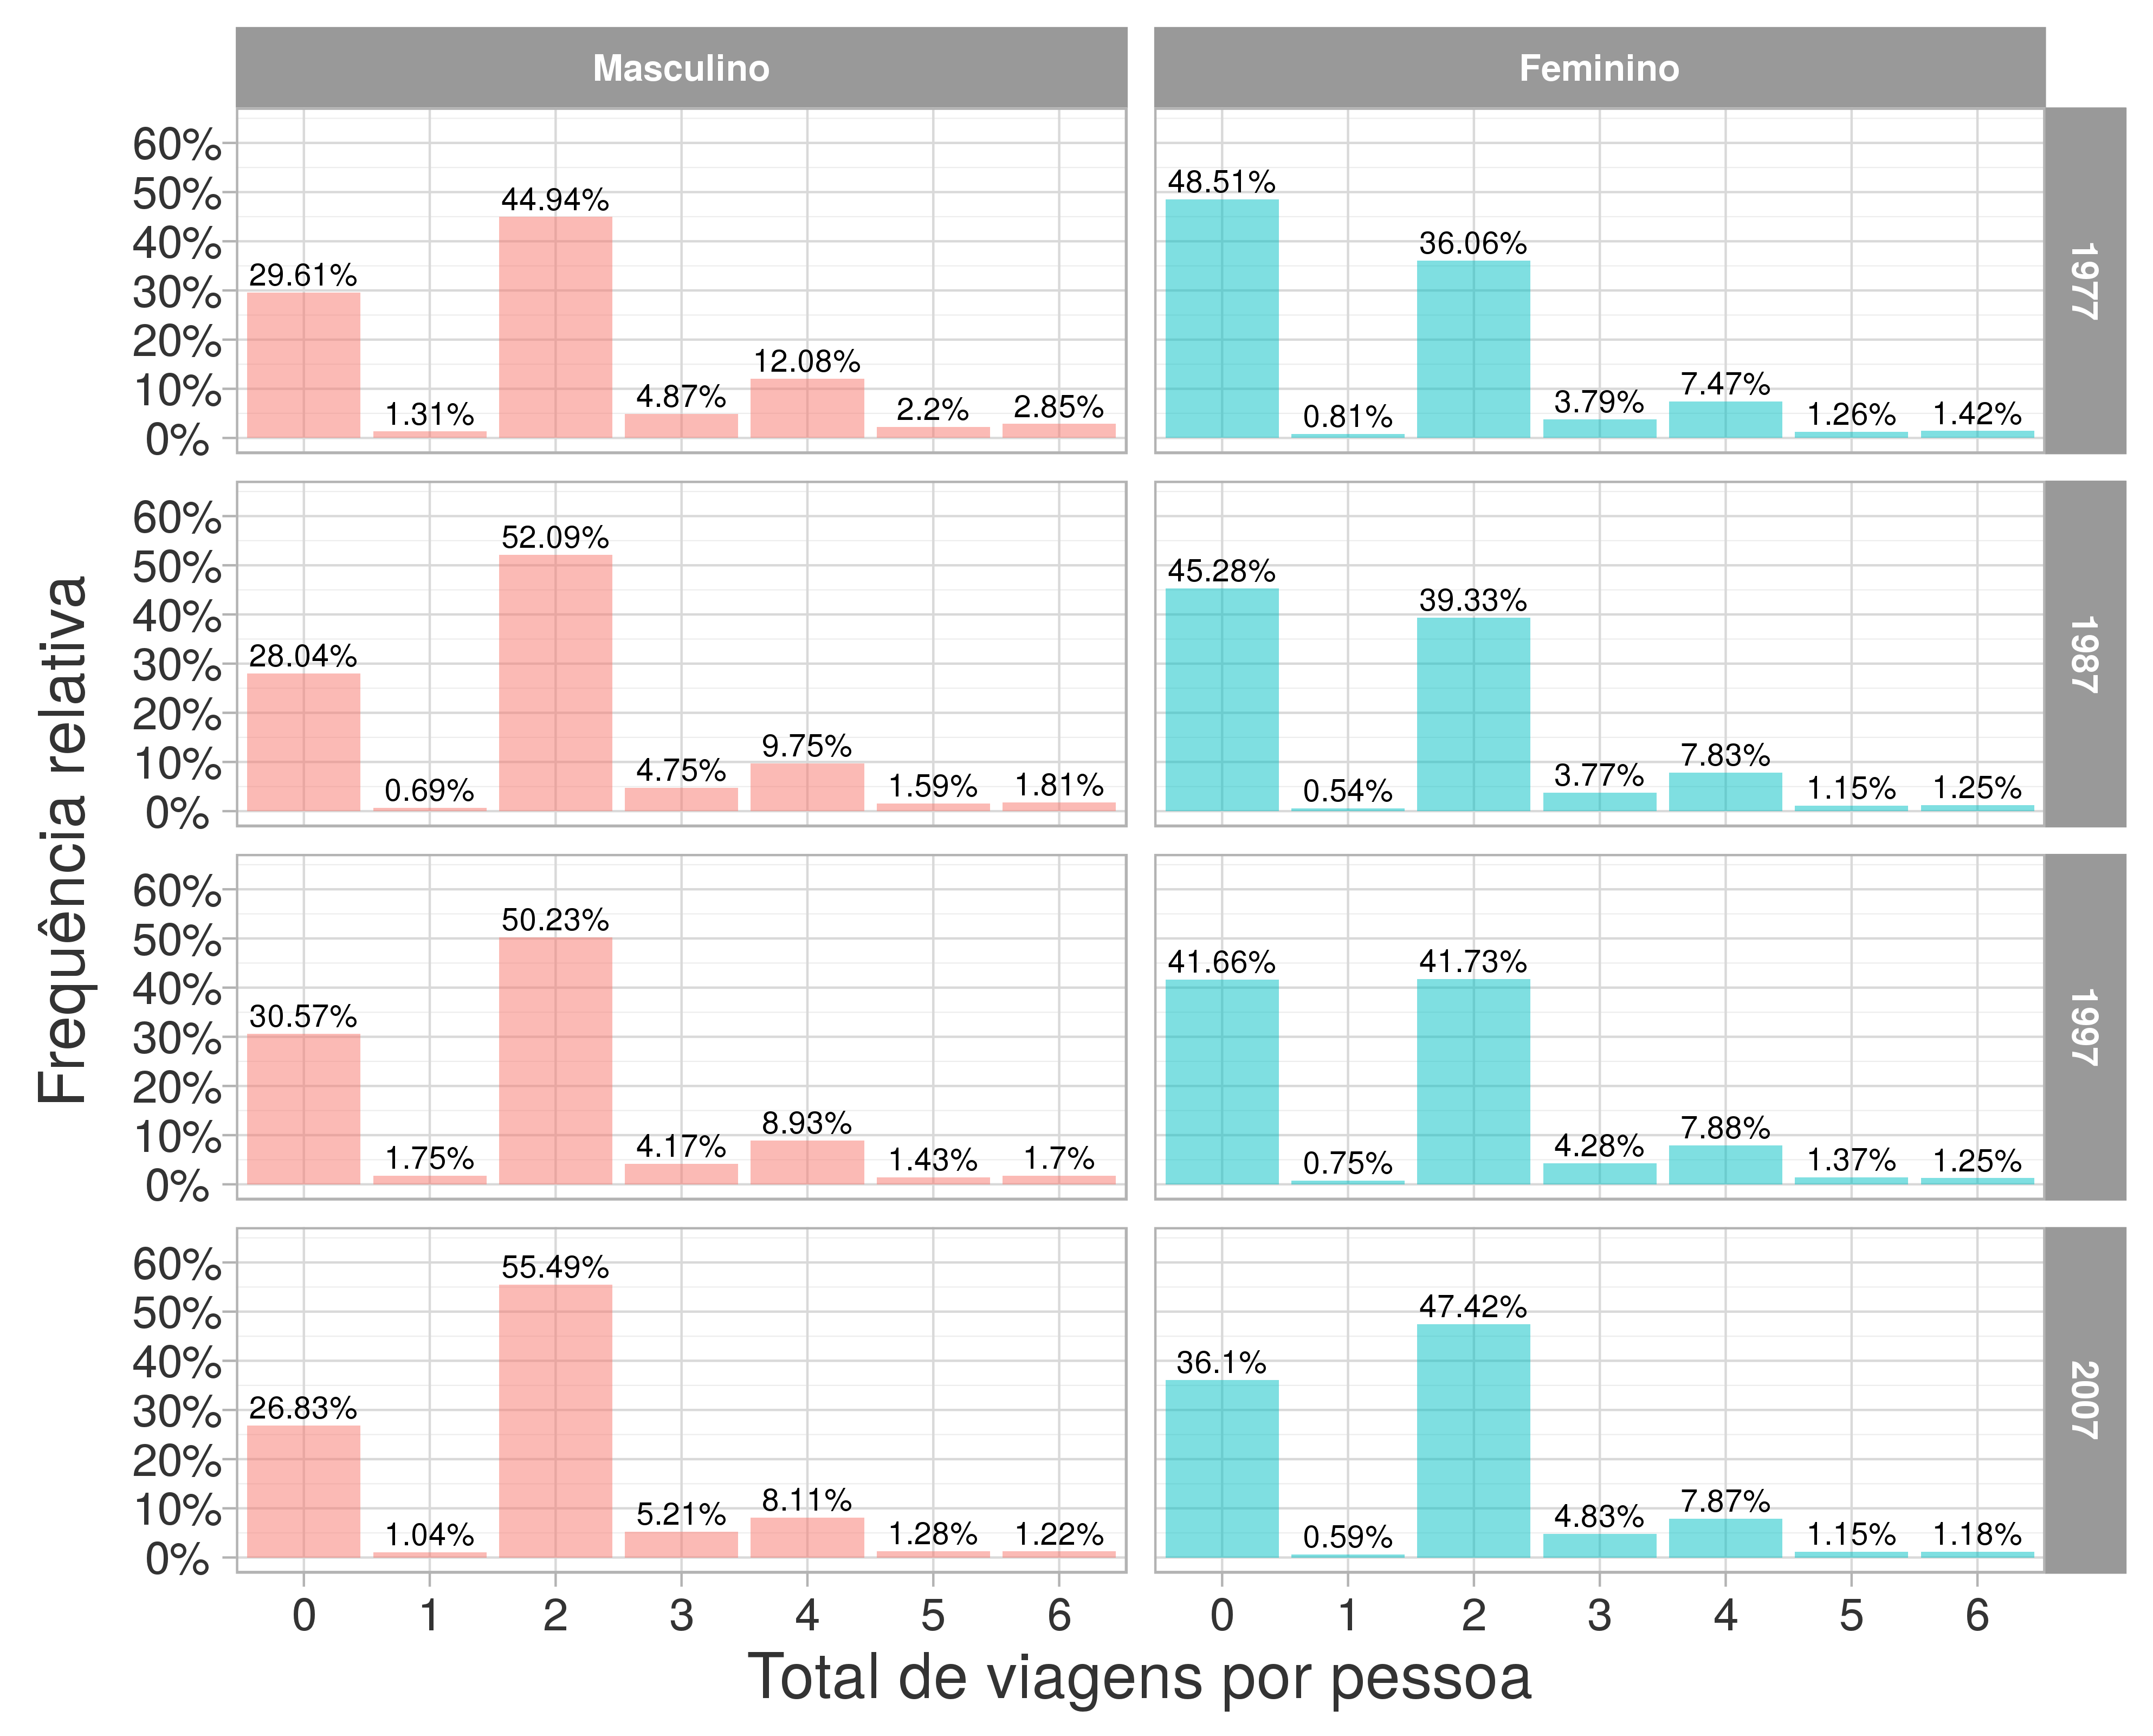
\includegraphics[width=1\textwidth]{./imagens/tot-viag-pess.png}%
    \end{center}%
%    \fonte{Compilação própria}
\end{grafico}%
% Estatísticas para registros com F_PESS==1 e SEXO
% Expandido com FE_PESS

\newpage
Ao focar no agregado da família, os valores das principais estatísticas (considerando os fatores de expansão para a população) da variável \textbf{FAM_VIAG_TOT} estão apresentados na Tabela \ref{tab:estat-fam-viag-tot}.
O número médio de viagens da família com ao longo do tempo, comportamento consistente tanto com a queda do número médio de viagens por pessoa (Tabelas \ref{tab:estat-tot-viag} e \ref{tab:estat-tot-viag-nao-nula}) quanto com a diminuição do tamanho da família (Tabela \ref{tab:estat-tot-pess}).
Aqui também os desvios padrão caem ao longo do tempo (tendência de menor dispersão de dados) e os valores de assimetria são positivos (maior concentração à esquerda e cauda longa à direita da distribuição). Os valores de curtose indicam que a distribuição não é normal.
Ao retirar aquelas famílias com total de viagens nulo (ninguém fez viagem), não se observam diferenças nas tendências das estatísticas, à exceção da mediana que em 1997 era 7 em 1997 e passa para 6 ao inserir famílias cujo total de viagens é zero.

\begin{table}[htb]
\centering
   \IBGEtab{%\renewcommand{\arraystretch}{1.5}%%\ABNTEXfontereduzida%
        \renewcommand{\arraystretch}{1.5}
        \caption{Estatísticas da variável ``FAM_VIAG_TOT'', por ano}
        \label{tab:estat-fam-viag-tot}
    }{%

    \begin{tabular}{ccccccc}
        \toprule
        \textbf{} & \multicolumn{5}{c}{\textbf{Considerando famílias em que há pela menos viagem}} & \multicolumn{1}{c}{\textbf{}} \\ \hline
        \textbf{ANO}   & \textbf{Média} & \textbf{Desvio Padrão} & \textbf{Mediana} & \textbf{Máximo} & \textbf{Assimetria} & \textbf{Curtose} \\ \midrule \midrule
        \textbf{1977}  & 8,97 & 6,00 & 8,00 & 59 & 1,36 & 2,90 \\ \hline
        \textbf{1987}  & 8,04 & 5,14 & 7,00 & 50 & 1,39 & 3,43 \\ \hline
        \textbf{1997}  & 7,68 & 4,80 & 7,00 & 45 & 1,29 & 2,85 \\ \hline
        \textbf{2007}  & 7,11 & 4,31 & 6,00 & 68 & 1,52 & 6,84 \\\bottomrule          

        \textbf{} & \multicolumn{5}{c}{\textbf{Considerando inclusive família em que ninguém fez viagem}} & \multicolumn{1}{c}{\textbf{}} \\ \hline
        \textbf{ANO}   & \textbf{Média} & \textbf{Desvio Padrão} & \textbf{Mediana} & \textbf{Máximo} & \textbf{Assimetria} & \textbf{Curtose} \\ \midrule \midrule
        \textbf{1977}  & 8,58 & 6,14 & 8,00 & 59 & 1,27 & 2,62 \\ \hline
        \textbf{1987}  & 7,71 & 5,28 & 7,00 & 50 & 1,27 & 3,05 \\ \hline
        \textbf{1997}  & 7,22 & 5,00 & 6,00 & 45 & 1,14 & 2,39 \\ \hline
        \textbf{2007}  & 6,62 & 4,53 & 6,00 & 68 & 1,28 & 5,38 \\\bottomrule

    \end{tabular}
    }{%
%		\fonte{Elaboração própria}
	}
\end{table}
% Estatísticas para registros com F_FAM==1, filtro por ANO
% Expandido com FE_FAM

\newpage
Nos campos MODO1, MODO2, MODO3 e MODO4 a categoria ``ônibus de linha'' inclui as categorias originais ``ônibus trólebus'', ``trólebus'', ``ônibus diesel'', ``ônibus'', ``ônibus município de São Paulo'', ``ônibus outros municípios'' e ``ônibus metropolitano''. A categoria ``ônibus escolar/empresa'' inclui também as categorias originais ``ônibus fretado'', ``escolar'', ``transporte escolar``. A categoria ``lotação/van'' inclui as categorias originais ``lotação/perua'', ``microônibus/van município de São Paulo'', ``microônibus/van outros municípios'' e ``microônibus/van metropolitano''. Vale destacar que para os anos de 1977 e 1987 foram levantados no máximo três modos, e para os anos 1997 e 2007, no máximo quatro modos para cada viagem.

Na Tabela \ref{tab:estat-modos} foram agrupados em ``alta capacidade'' os modos metroferroviários (metrô e trem), em ``ônibus'' todos os tipos de ônibus (de linha, escolar, de empresas, lotações e vans), em ``passageiro de automóvel'' os passageiros de automóvel particular e também de táxis, em ``Outros'' as viagens realizadas por motocicletas e bicicletas pois estas foram diagnosticadas apenas para 2007. Nesta tabela estão apresentadas as frequências relativas destes agrupamentos para o \textbf{MODO1} (primeiro modo utilizado na viagem) e também para o \textbf{MODO2} (segundo modo utilizado), buscando avaliar a divisão modal por ano, para quem realizou viagem. Assim, para o primeiro modo o total soma 100\% em todos anos, mas o total por ano do segundo modo em diante não necessariamente, porque nem todas viagens utilizaram mais de um modo.


\begin{table}[htb]
\centering
   \IBGEtab{%\renewcommand{\arraystretch}{1.5}%%\ABNTEXfontereduzida%
        \renewcommand{\arraystretch}{1.5}
        \caption{Frequência relativa das variáveis ``MODO1'' e ``MODO2'', por ano}
        \label{tab:estat-modos}
    }{%

    \begin{tabular}{cccccccc}
        \toprule
        \textbf{MODO 1} & \textbf{Alta}       & \textbf{}       & \textbf{Dirigindo} &  \textbf{Passageiro}  & \textbf{}     & \textbf{}  & \textbf{} \\
        \textbf{ANO}    & \textbf{Capacidade} & \textbf{Ônibus} & \textbf{Automóvel} & \textbf{de Automóvel} & \textbf{A pé} & \textbf{Outros} & \textbf{Total} \\ \midrule \midrule
        \textbf{1977}  & 3,0\% & 41,7\% & 15,4\% & 11,3\% & 28,0\% & 0,8\% & 100\% \\ \hline
        \textbf{1987}  & 4,7\% & 30,5\% & 17,2\% &  9,7\% & 36,2\% & 1,7\% & 100\% \\ \hline
        \textbf{1997}  & 6,4\% & 28,9\% & 20,5\% & 10,8\% & 34,4\% & 1,3\% & 100\% \\ \hline
        \textbf{2007}  & 7,0\% & 31,8\% & 19,2\% &  8,6\% & 33,1\% & 2,9\% & 100\% \\\bottomrule          

        \textbf{MODO 2}      & \textbf{Alta}       & \textbf{}       & \textbf{Dirigindo} &  \textbf{Passageiro}  & \textbf{}     & \textbf{}  & \textbf{} \\
        \textbf{ANO}   & \textbf{Capacidade} & \textbf{Ônibus} & \textbf{Automóvel} & \textbf{de Automóvel} & \textbf{A pé} & \textbf{Outros} & \textbf{Total} \\ \midrule \midrule
        \textbf{1977}  & 2,0\% & 7,0\% & 0,1\% & 0,2\% & - & 0,0\% &  9,2\% \\ \hline
        \textbf{1987}  & 3,6\% & 6,5\% & 0,1\% & 0,1\% & - & 0,0\% & 10,3\% \\ \hline
        \textbf{1997}  & 3,5\% & 5,9\% & 0,0\% & 0,1\% & - & 0,0\% &  9,5\% \\ \hline
        \textbf{2007}  & 4,2\% & 8,2\% & 0,1\% & 0,1\% & - & 0,0\% & 12,5\% \\\bottomrule    
      
    \end{tabular}
    }{%
%		\fonte{Elaboração própria}
	}
\end{table}
% Estatísticas para registros com F_VIAG==1
% Expandido com FE_VIAG

Em relação à utilização do automóvel, sua proporção sobe cerca de 5\% de 1977 até 1997 e cai pouco mais de 1\% em 2007, talvez por conta dos congestionamentos cada vez mais frequentes e da evolução do sistema de transporte coletivo público da RMSP. Quando utilizado, o carro é quase sempre o único modo da viagem.
Os ônibus têm uma queda de $\sim$ 13\% pontos percentuais entre 1977 e 1997, com recuperação de $\sim$ 3\% em 2007. Quem deixou de utilizar o ônibus nas primeiras 3 décadas passou a utilizar a caminhada como método de deslocamento ($\sim$ 6\%), ou o carro ($\sim$ 5\%) o ainda o transporte coletivo de alta capacidade ($\sim$ 3\%).
Os modos metrô e trem vêm recebendo um incremento de viagens década a década, saindo de 3\% em 1977 para 7\% em 2077. A contribuição baixa deste modo, apesar de sua alta capacidade, deve-se provavelmente à cobertura insuficiente de pouca capilaridade no tecido urbano.
Vale ressaltar que ``alta capacidade'' é o único modo que tem sua utilização ainda muito presente como segundo modo (relação MODO1/MODO2 $\sim$ 1,5) - as viagens de ônibus são reduzidas pelo menos da ordem de um quarto, as de carro e outros caem a quase 0\% no segundo modo.
Isto significa que as viagens com metrô e trem são mais frequentemente precedidas de viagens com outro modo (principalmente ônibus), funcionando como tronco numa lógica de sistema tronco-alimentador.
As viagens a pé aumentaram percentualmente entre 1977 e 1997 e caíram em 2007, talvez pelas distâncias necessárias de viagem dado o crescimento da área metropolitana de São Paulo. Conforme o conceito de viagem a pé anteriormente exposto, não haverá modo a pé nos modos 2, 3 ou 4.
As tabelas de contingência dos modos 3 e 4 não serão apresentadas por serem pouco significativos no contexto geral: o modo 3 varia de 0,9\% (em 1977) a 2,8\% (2007) do total de viagens, sendo predominante o modo ônibus; o modo 4, só existente em 1997 e 2007, corresponde ao total de 0,4\% das viagens realizadas.

Os Gráficos \ref{graf:freq-modo1} e \ref{graf:freq-modo2} apresentam a segmentação por sexo dos modos 1 e 2 de viagem, respectivamente.
No primeiro modo de viagem, as viagens a pé são o modo mais frequente para as mulheres em 1987, 1997 e 2007, somente em 1977 o ônibus era mais frequentemente utilizado por elas.
Para os homens o modo mais frequente em 1977 e 2007 é o ônibus, e em 1987 e 1997, a pé.
O modo outros é o menos frequente em 1977, 1987 e 1997 para ambos sexos; em 2007, eles superam a alta capacidade, provavelmente porque a expressividade do transporte por motocicleta e bicicleta passou a ser mais expressiva e foi incluída na categoria outros.
Comparando ambos sexos por categoria do primeiro modo:
\begin{compactitem}[]
\item (i) As mulheres sempre fizeram mais viagens a pé que os homens: a diferença de 6,7 pontos percentuais de 1977 aumenta para 11,3 em 1987, cai para 7,9 em 1997 e sobe novamente em 2007 para 8,8\%.
\item (ii) A utilização feminina do ônibus é quase sempre superior á masculina, exceto em 1987, ano em que as proporções praticamente se igualam e desde quando a diferença vem aumentando com o tempo.
\item (iii) É na utilização do automóvel em que residem as diferenças mais gritantes entre os gêneros: homens predominantemente motoristas e mulheres, passageiras. O destaque aqui reside no fato que entre 1997 e 2007, dentro do grupo de mulheres, elas passaram a dirigir mais do que ser passageiras de automóvel.
\item (iv) O transporte de alta capacidade gira em torno de 2,5\% a 5,5\% do \textit{share} modal, com o homem tendo uma utilização um pouco mais frequente dentro do seu grupo do que as mulheres, mais devido ao trem (cujos percentuais dos homens são sempre superiores aos das mulheres) do que ao Metrô (onde os percentuais das mulheres supera o dos homens a partir de 1997).
\end{compactitem}

\begin{grafico}[htb]%
    \caption{\label{graf:freq-modo1}Proporção das viagens do sexo feminino e do sexo masculino, segundo o primeiro modo da viagem, por ano}%
    \begin{center}%
        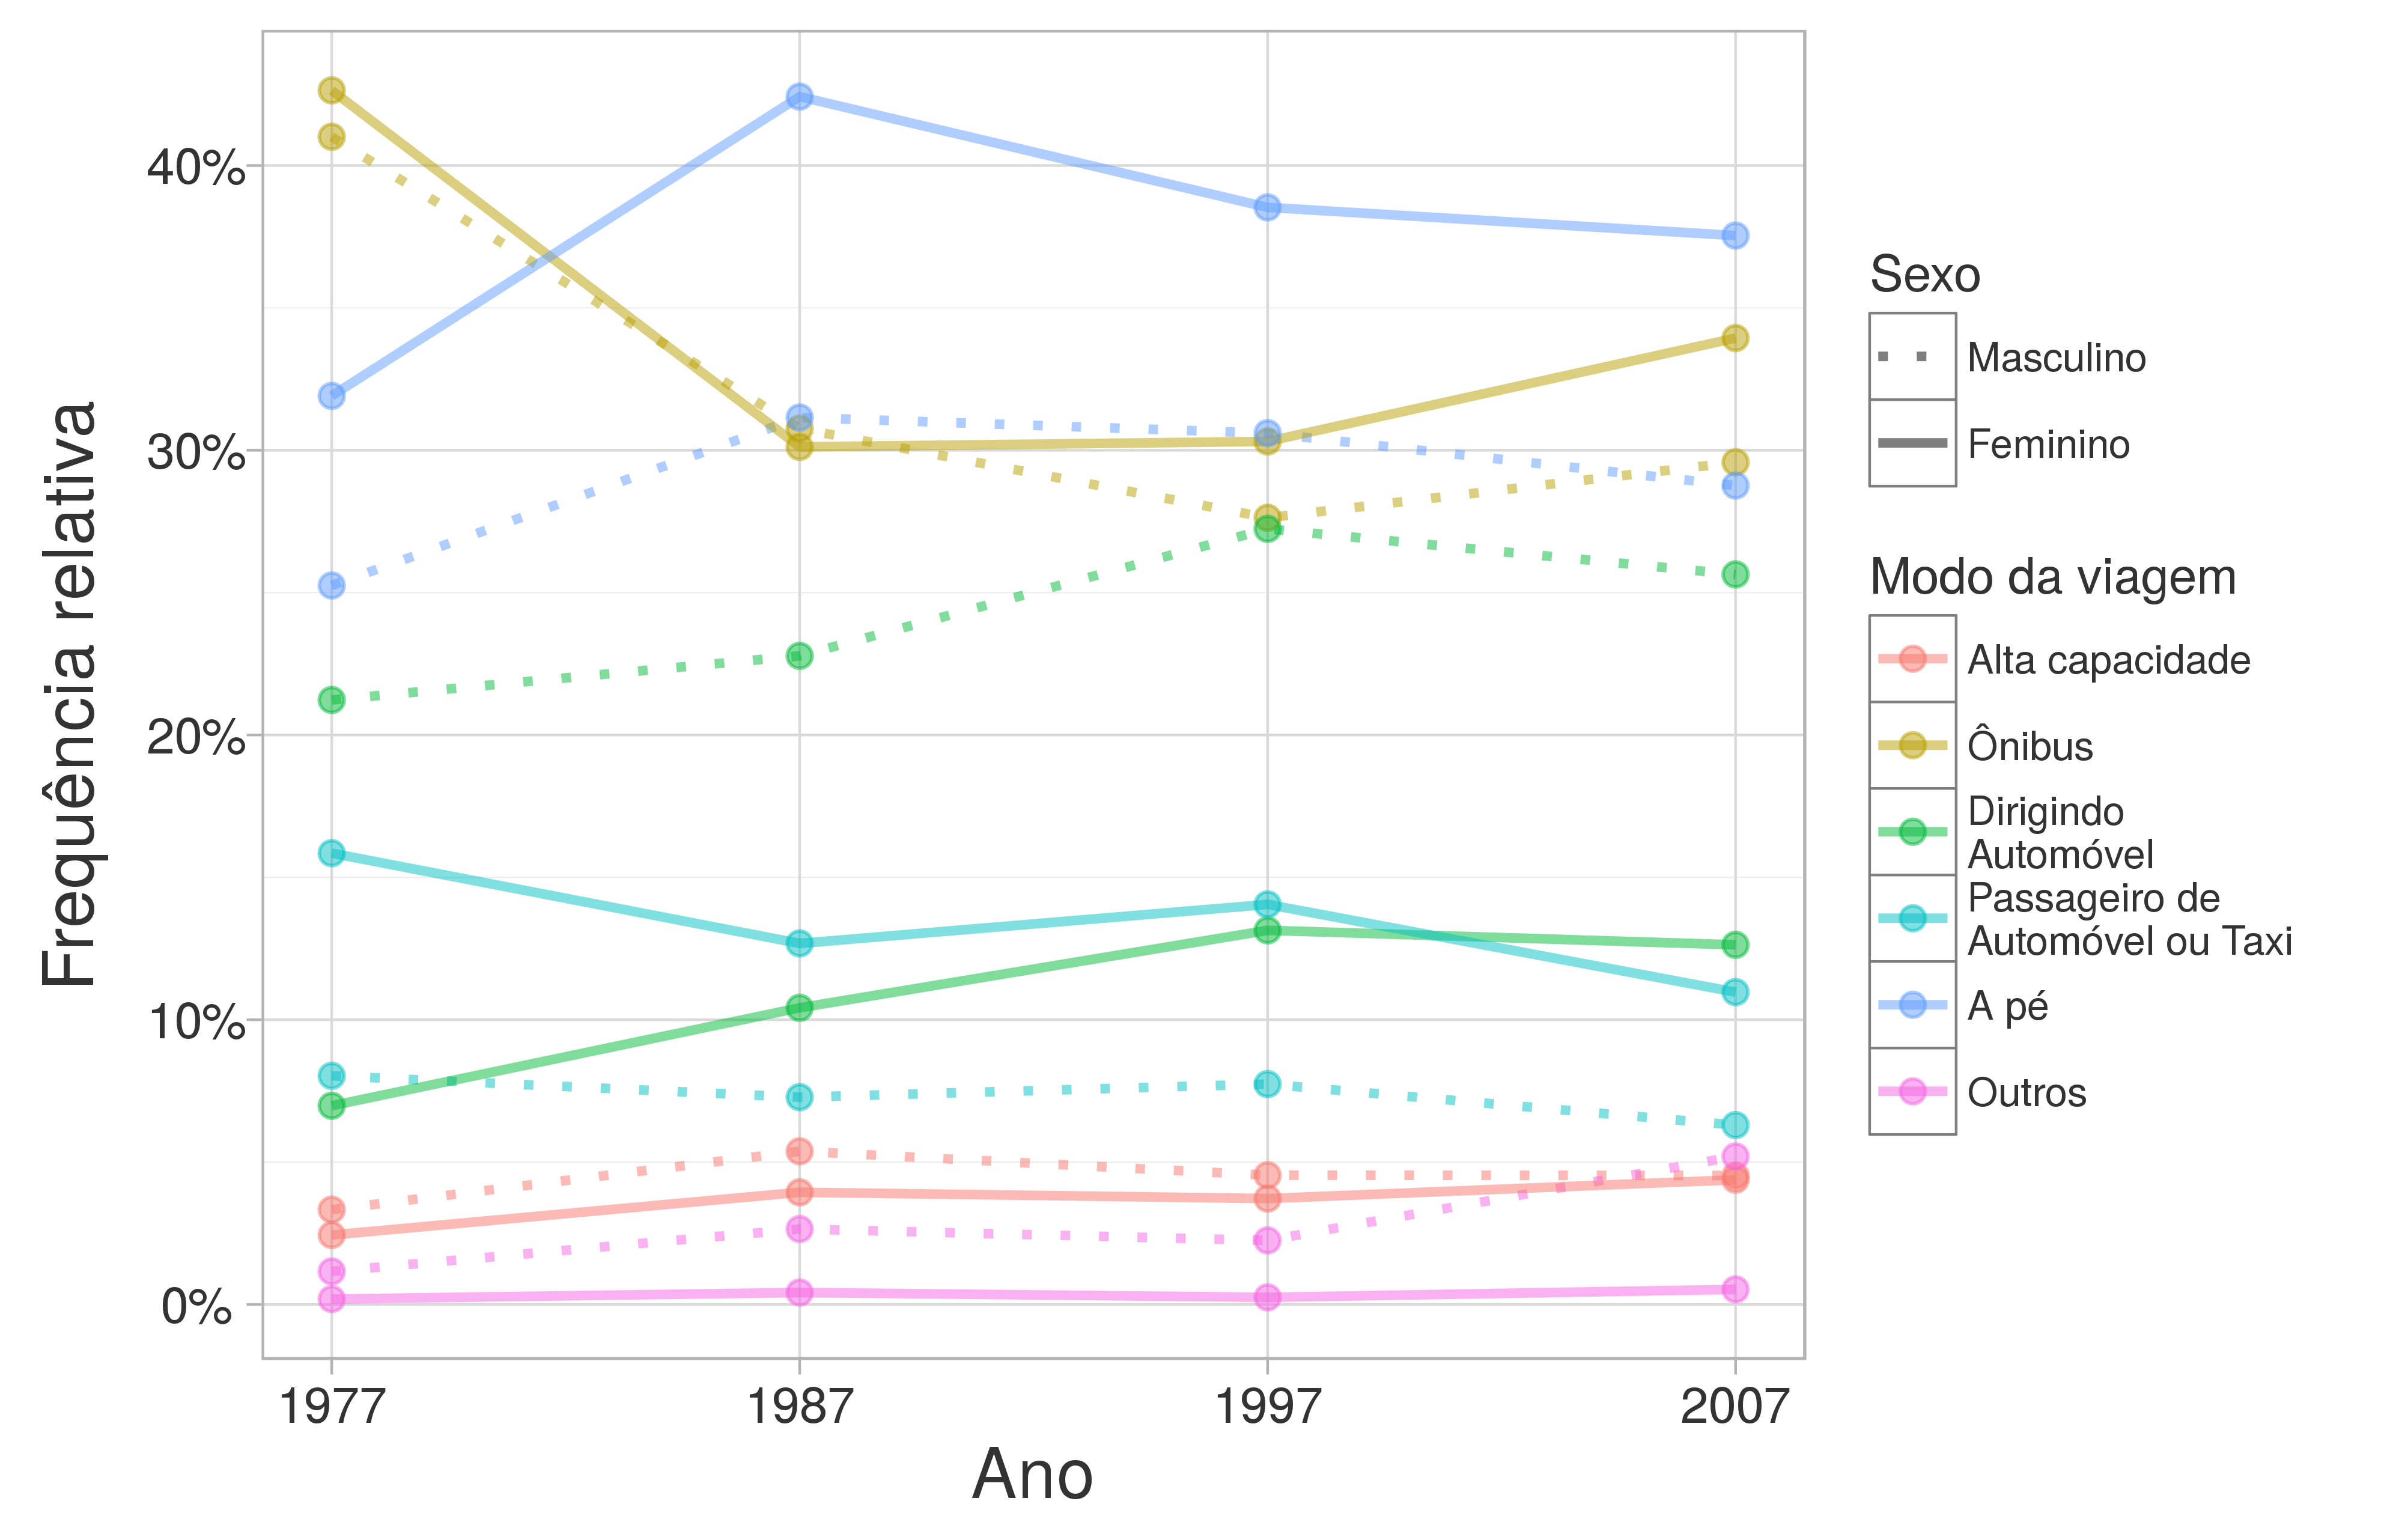
\includegraphics[width=1\textwidth]{./imagens/freq-modo1.png}%
    \end{center}%
%    \fonte{Compilação própria}
\end{grafico}%
% Estatísticas para registros com F_VIAG==1 e SEXO
% Expandido com FE_VIAG

Analisando agora as categorias do segundo modo, por sexo:
\begin{compactitem}[]
\item (i)  As duas categorias que apresentam relevância como segundo modo de transporte equivalem aos modos coletivos ônibus e alta capacidade (metrô e trem), os demais modos ou não foram considerados (por exemplo, a pé) ou não são muito significativos (automóvel e outros).
\item (ii) A utilização feminina do ônibus, como segundo modo da viagem, é inferior à masculina entre 1977 e 1997, ao contrário do que ocorria com o primeiro modo. Em 2007 a situação se altera, quando pessoas do sexo feminino passam a utilizar mais frequentemente o ônibus.
\item (iii) A frequência do uso de alta capacidade é mais expressiva no conjunto do modo 2, embora ainda seja menor que a do ônibus em todos os anos e para ambos sexos.
\item(iv) Para as mulheres, de 1977 para 1987, parece ter havido uma troca modal no segundo modo: houve queda de $\sim$ 1\% no uso do ônibus e aumento também de $\sim$ 1\% no uso de alta capacidade. Foi nesse período em que houve a primeira expansão da rede metroferroviária para a zona leste (trecho Sé-Penha).
\end{compactitem}

\begin{grafico}[htb]%
    \caption{\label{graf:freq-modo2}Proporção das viagens do sexo feminino e do sexo masculino, segundo o segundo modo da viagem, por ano}%
    \begin{center}%
        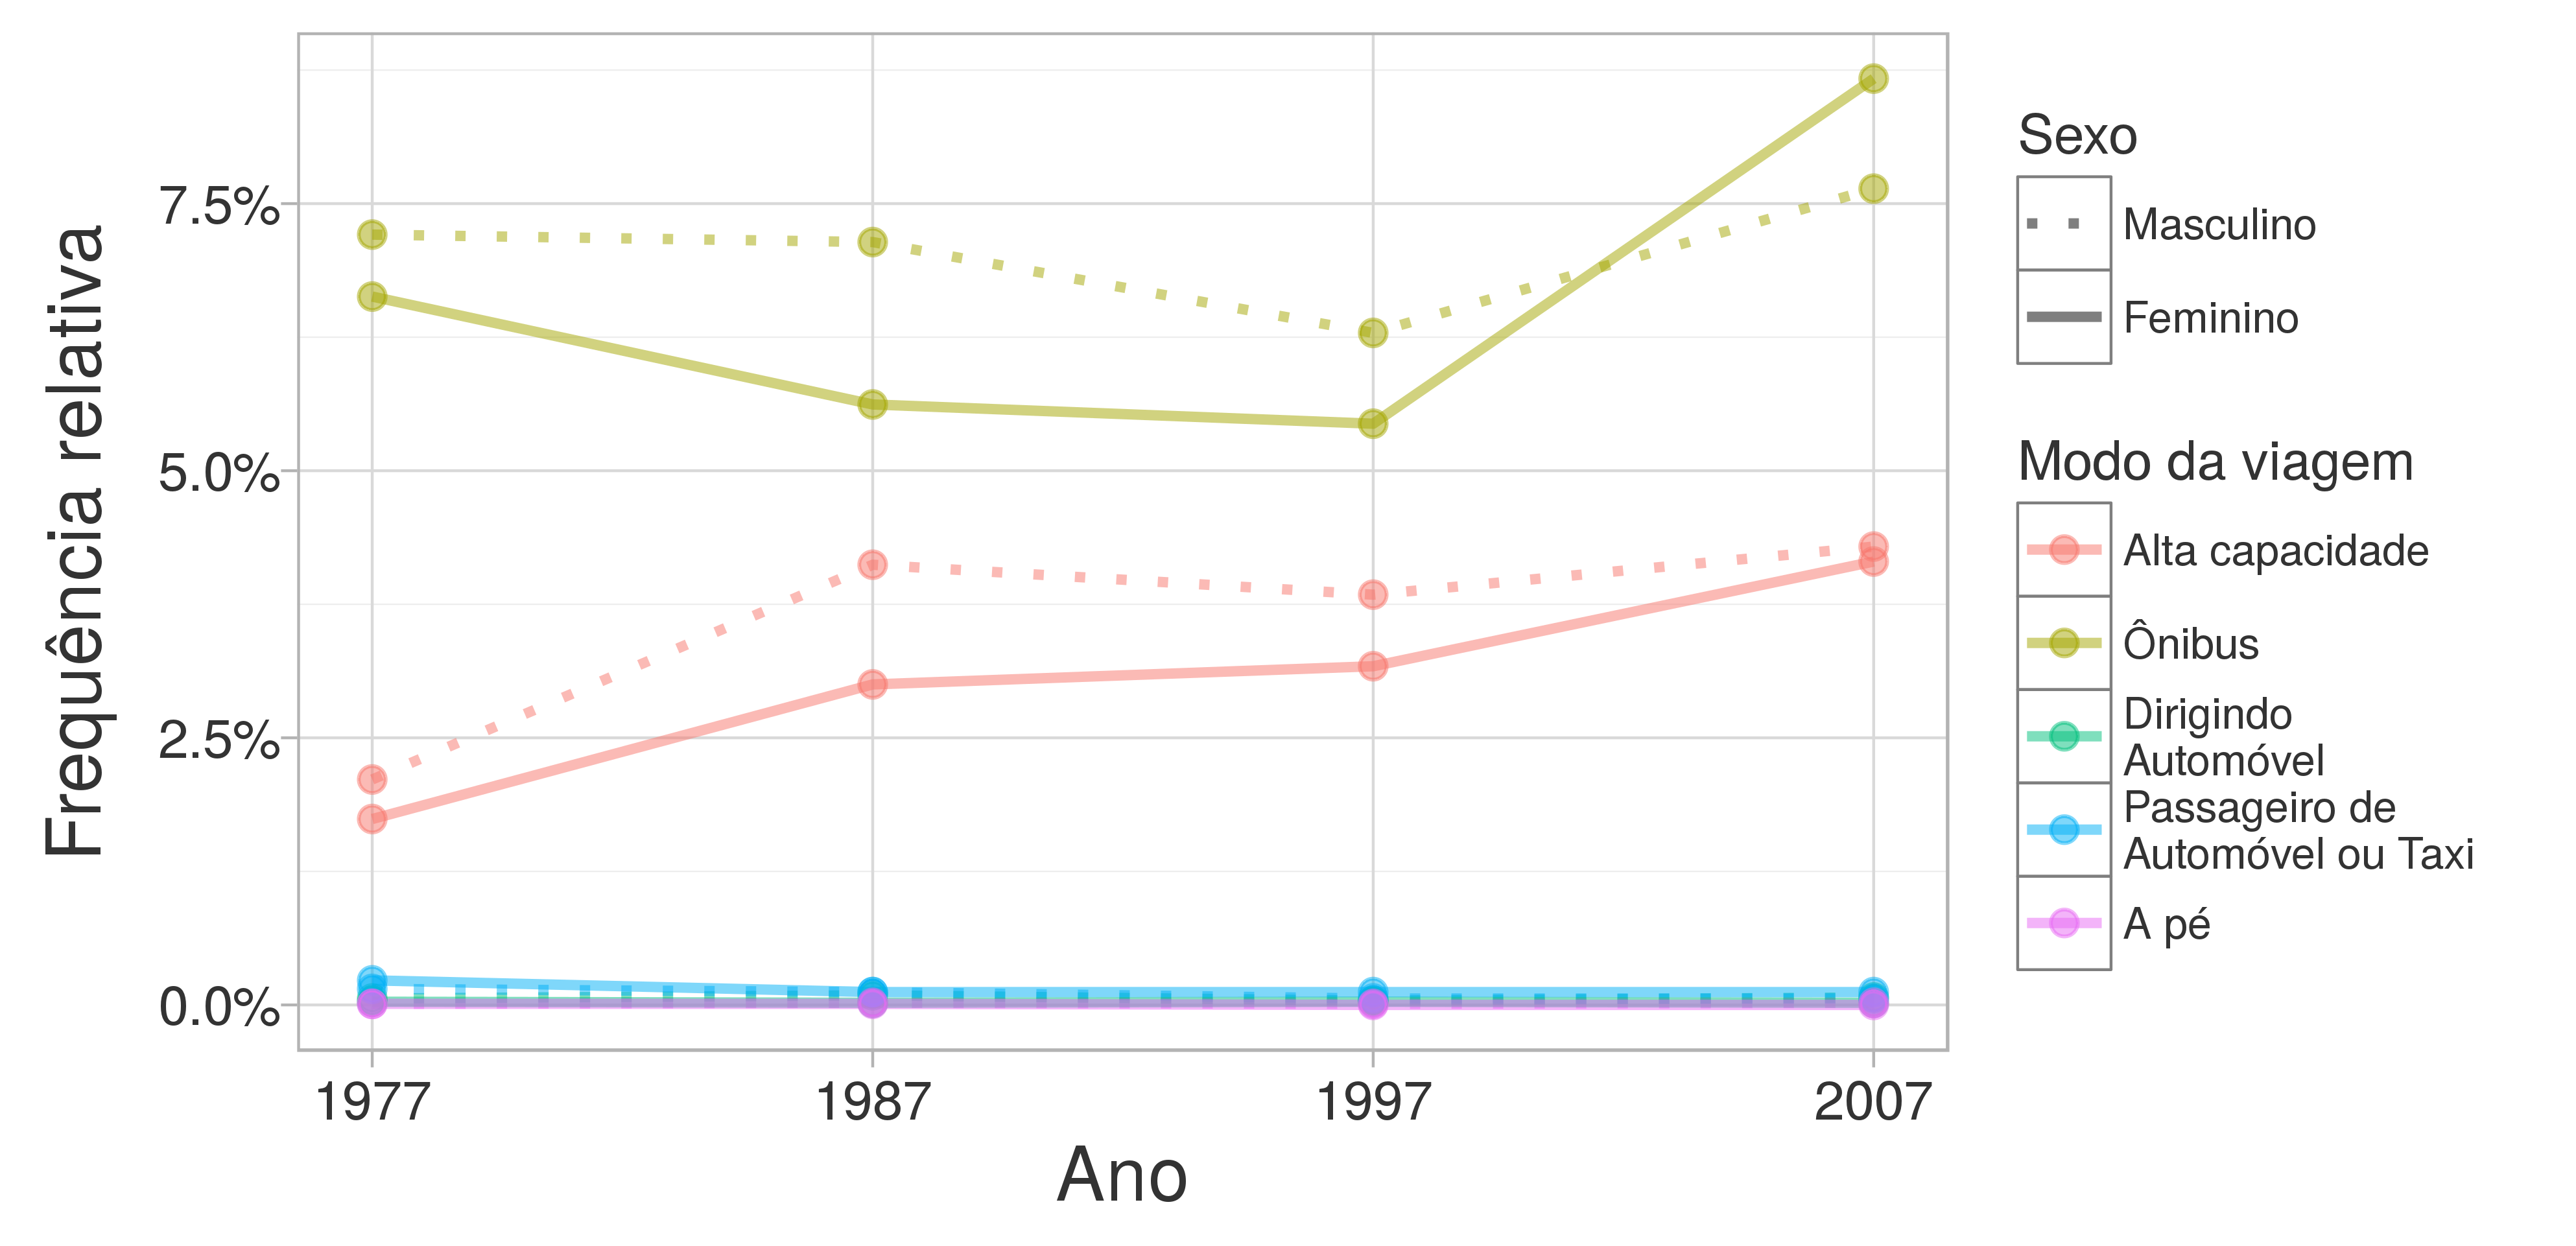
\includegraphics[width=1\textwidth]{./imagens/freq-modo2.png}%
    \end{center}%
%    \fonte{Compilação própria}
\end{grafico}%
% Estatísticas para registros com F_VIAG==1 e SEXO
% Expandido com FE_VIAG

\clearpage

É possível também analisar os modos agregando os modos em ``coletivo'', ``individual'' e ``a pé'', o que já fora feito na variável \textbf{TIPO_VIAG}, cujas frequências relativas são apresentadas na Tabela \ref{tab:estat-tipo-viag}.
O transporte individual cresceu de 1977 a 1997 e recuou um pouco em 2007.
O transporte coletivo decresceu entre 1977 e 1987, mas a uma taxa bem maior que o crescimento do individual, o que significa que essas viagens deixaram de ser feitas de transporte coletivo para, principalmente, serem feitas a pé ou, com menor frequência, de carro.
Entre 1987 a 1997 tanto o transporte coletivo como o modo a pé sofrem ligeiras quedas (em torno de 2 pontos percentuais), período em que o transporte individual aumenta sua taxa de crescimento. Neste ano o cenário da divisão modal fica quase equitativamente dividido com cerca de um terço para cada uma das três categorias.
Em 2007 a forma de deslocamento a pé sofre ligeira queda ($\sim$ 1\%), o transporte individual também cai ($\sim$ 2,5\%) e essas viagens passam a ser feitas pelo transporte coletivo que assume proporção um pouco superior à que tinha em 1987.

\begin{table}[htb]
\centering
   \IBGEtab{%\renewcommand{\arraystretch}{1.5}%%\ABNTEXfontereduzida%
        \renewcommand{\arraystretch}{1.5}
        \caption{Frequência relativa da variável ``TIPO_VIAG'', por ano}
        \label{tab:estat-tipo-viag}
    }{%

    \begin{tabular}{cccc}
        \toprule
        \textbf{ANO}   & \textbf{Coletivo} & \textbf{Individual} & \textbf{A pé} \\ \midrule \midrule
        \textbf{1977}  & 45,0\%            & 27,0\%              & 28,0\%  \\ \hline
        \textbf{1987}  & 35,6\%            & 28,2\%              & 36,2\%  \\ \hline
        \textbf{1997}  & 33,3\%            & 32,3\%              & 34,4\%  \\ \hline
        \textbf{2007}  & 36,5\%            & 29,5\%              & 33,1\%  \\ \bottomrule          
    \end{tabular}
    }{%
%		\fonte{Elaboração própria}
	}
\end{table}
% Estatísticas para registros com F_VIAG==1
% Expandido com FE_VIAG

O Gráfico \ref{graf:freq-tipo-viag} apresentam a segmentação por sexo do modo (agregado) de viagem.
Comparando ambos sexos por categoria do primeiro modo:
\begin{compactitem}[]
\item (i) Em 1977, 45,4\% das mulheres usavam o transporte coletivo, 31,9\% deslocavam-se a pé e 22,7\% usavam transporte individual. Em 1987, para elas, o transporte individual permanece no mesmo patamar ($\sim$ 23,2\%) e ocorre uma migração do coletivo para o a pé com 34,4\% e 42,4\%, respectivamente.
\item (ii) Em 1977, 44,7\% dos homens usavam o transporte coletivo, 30,1\% o individual e 25,3\% deslocavam-se a pé. Em 1987, para eles, o transporte individual cresceu ($\sim$ 32,3\%) e as viagens a pé também ($\sim$ 31,2\%) indicando uma migração do transporte coletivo (36,5\%) para estes modos.
\item (iii) Entre 1987 e 1997, a proporção de mulheres a usar o transporte coletivo permanece inalterada, mas ocorre uma migração do modo a pé para o transporte individual.
\item (iv) Entre 1987 e 1997, a proporção de homens a usar o transporte individual continua aumentando (para 37\%), superando a participação do coletivo (32,4\%), enquanto as viagens a pé permanecem no mesmo patamar.
\item (v) Entre 1997 e 2007, a proporção do uso feminino do transporte coletivo cresce (para 38,7\%) indicando migração para este modo das viagens advindas, especialmente, do transporte individual (que cai para 23,6\%) e, em menor medida, do modo a pé (com 37,5\%). 
\item (vi) Entre 1997 e 2007, a proporção do uso masculino do transporte coletivo também cresce (para 34,4\%) indicando migração para este modo das viagens advindas tanto do transporte individual (que cai para 35,4\%) como do modo a pé (com 28,8\%).
\end{compactitem}
% Em 2007 não fecha 100% porque havia no banco uns casos de TIPO_VIAG=4, cujo significado desconheço pois valor não consta do layout

\begin{grafico}[htb]%
    \caption{\label{graf:freq-tipo-viag}Proporção das viagens do sexo feminino e do sexo masculino, segundo o modo da viagem (agregado), por ano}%
    \begin{center}%
        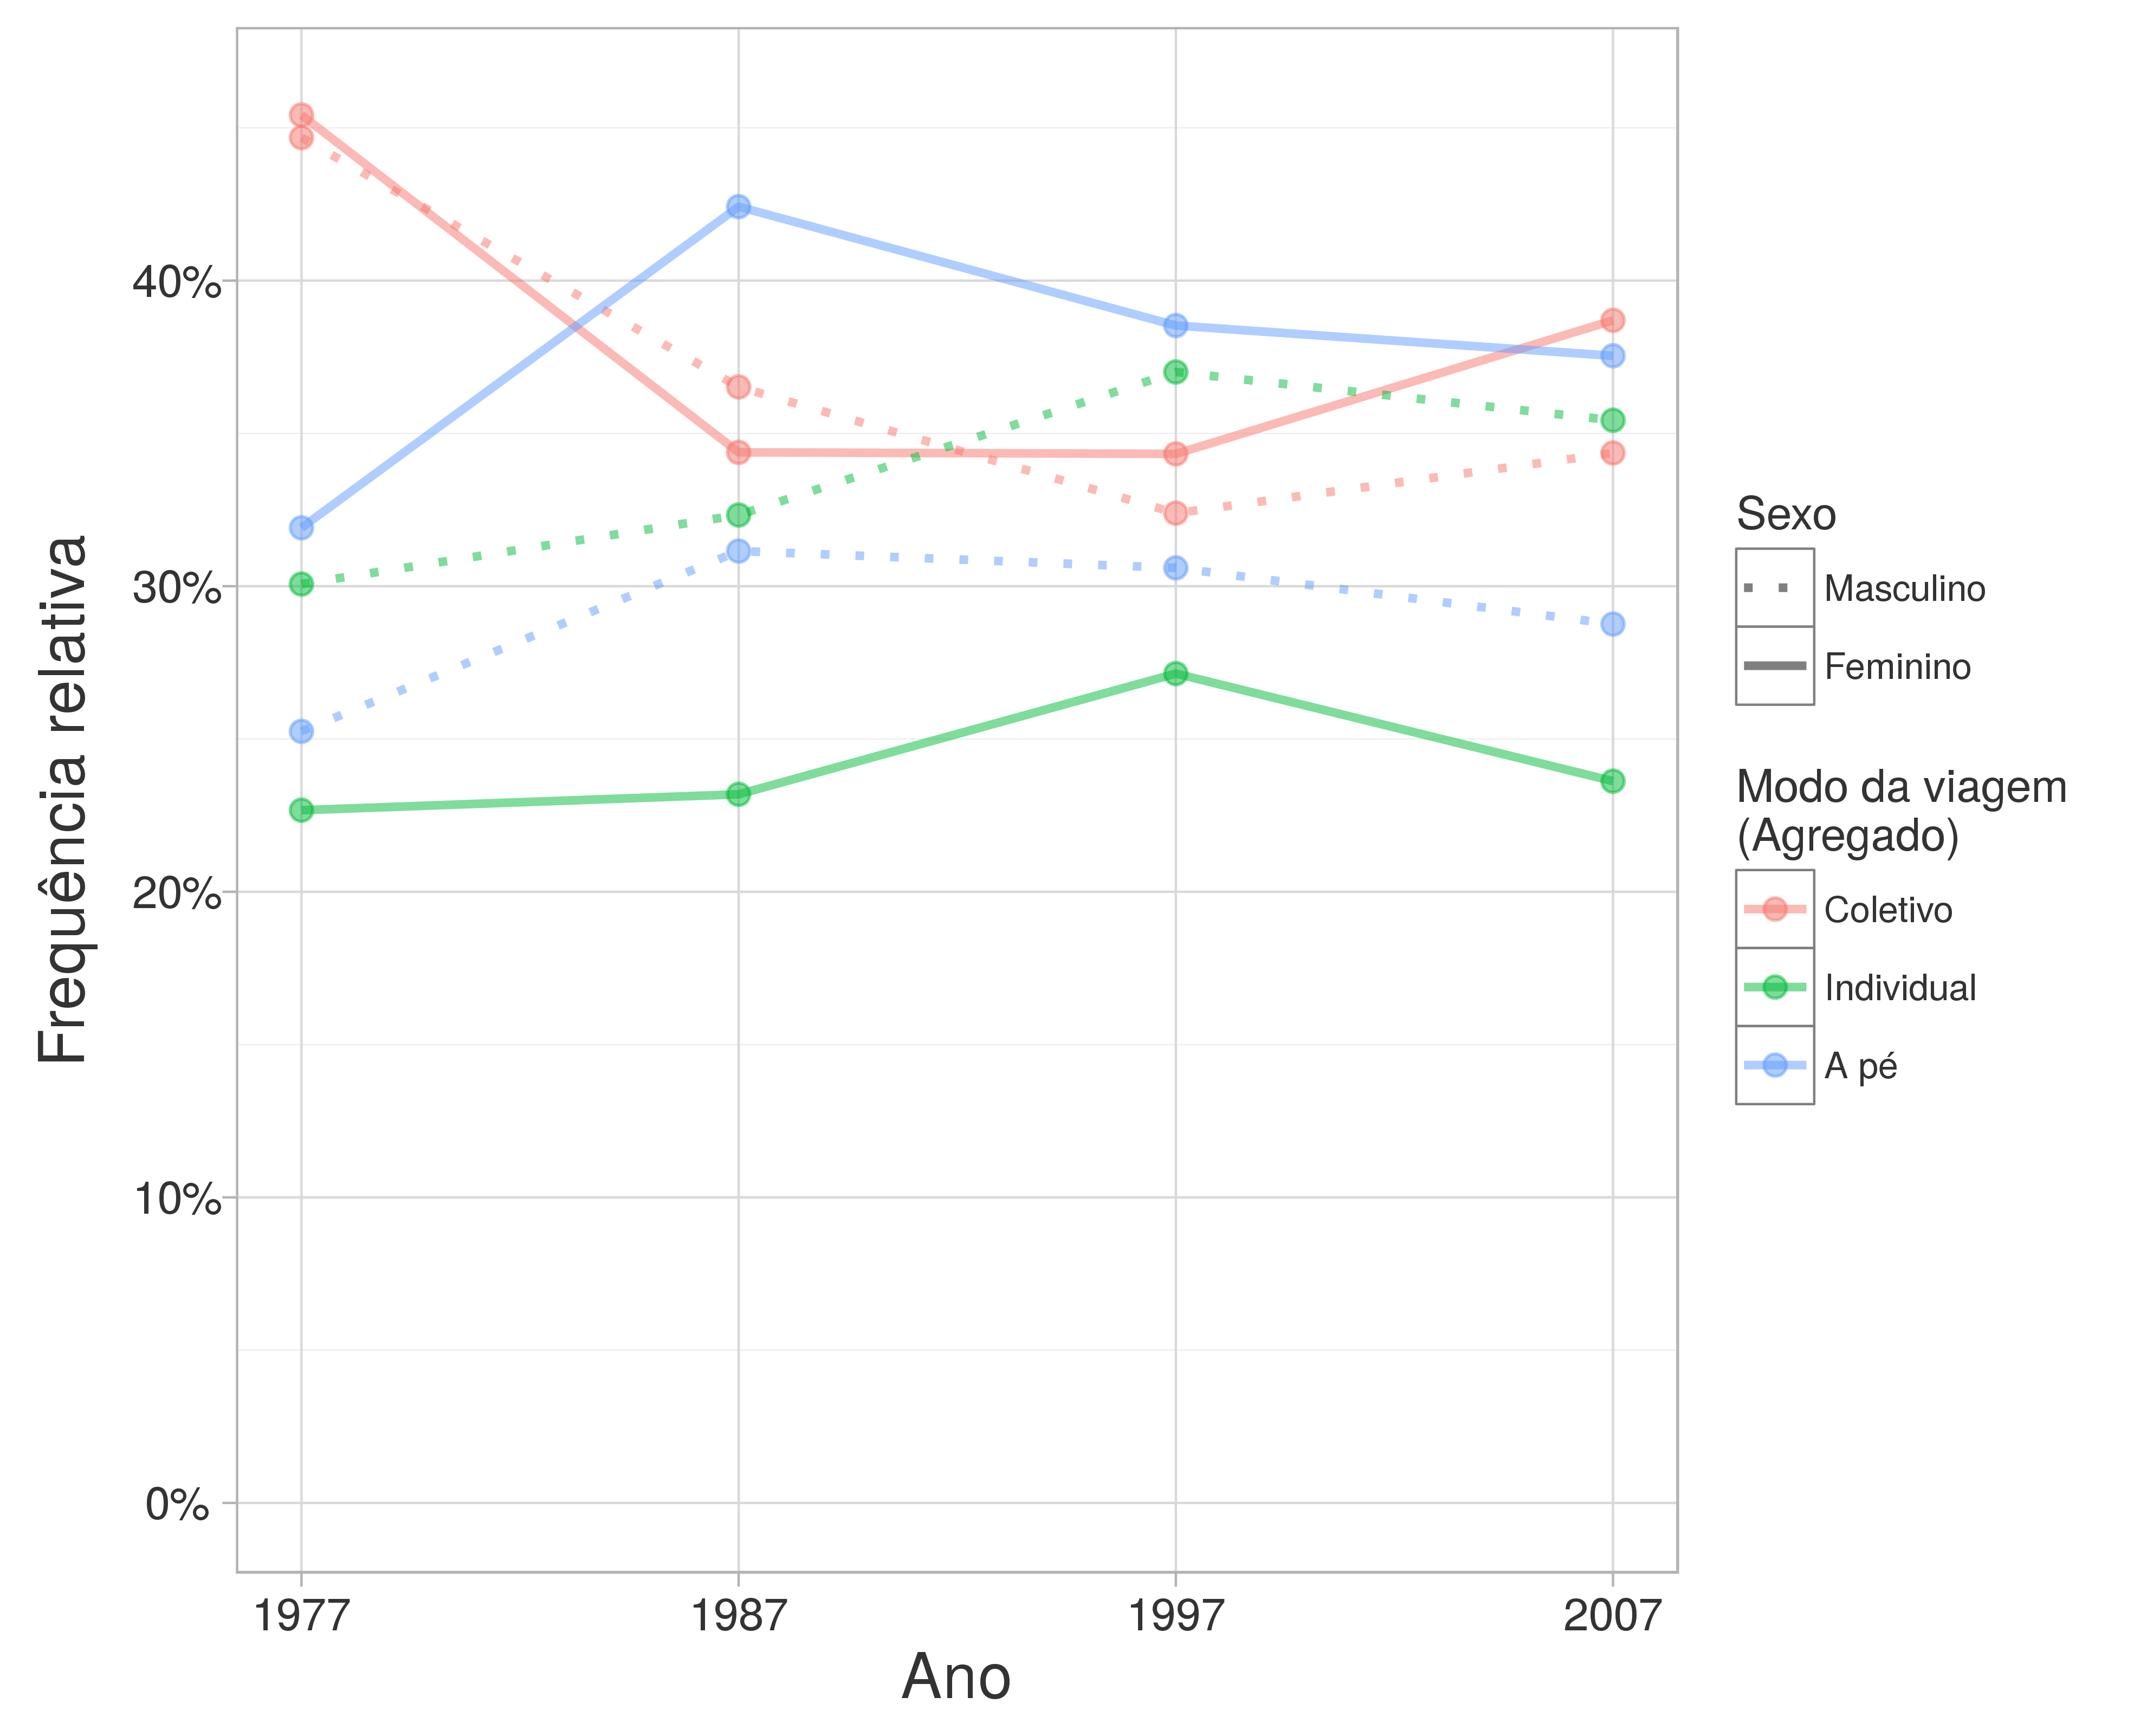
\includegraphics[width=1\textwidth]{./imagens/freq-tipo-viag.png}%
    \end{center}%
%    \fonte{Compilação própria}
\end{grafico}%
% Estatísticas para registros com F_VIAG==1 e SEXO
% Expandido com FE_VIAG

Para as variáveis de motivo (\textbf{MOTIVO_ORIG} e \textbf{MOTIVO_DEST}) foi criada a categoria ``servir passageiro''. Para tanto, olhava-se a variável de cada OD ``servir passageiro na origem''; caso fosse afirmativo (1), a categoria adotada é ``servir passageiro'', porque o que motiva esse deslocamento é o motivo de outrem, não o da pessoa respondente. Caso contrário, adota-se o motivo de origem indicado originalmente na base de dados. Tal procedimento foi realizado com as bases de 1997 e 2007. A base de 1977 já conta com a categoria ``servir passageiro''. A base de 1987 é a única que não possui informações suficientes para identificar esse motivo de viagem.

Será explorada a variável motivo no destino porque essa variável indica a atividade fim que gerou o deslocamento.
A Tabela \ref{tab:estat-motivo-dest} foi feita expandindo as viagens com o FE_VIAG, consequentemente consideradas apenas as viagens realizadas (cujo FE_VIAG não foram iguais a zero).
Observa-se que o motivo ``residência'' corresponde à maior parte das viagens (cerca de 45\%) realizadas, se alterando pouco ao longo dos anos - resultado próximo ao esperado (pouco menos de 50\%) dado que o comportamento de deslocamentos da demanda tem a residência como base, ou seja, é para onde a maior parte das pessoas retornam após executar alguma outra atividade.
O segundo motivo mais frequente é ``trabalho'' girando em torno dos 23,5\% e também oscilando pouco (1\%) ao longo dos anos, seguido por ``educação'', que cresce de 1977 (13,2\%) para 1987 (16,9\%) e depois decresce em 1997 (14\%) e se mantém em 2007 (14\%).
Assim, trabalho, educação e residência são os motivos de pouco mais de 80\% das viagens em todos os anos.
A proporção das viagens motivo ``manutenção-compras'' cresce de 1977 (3,9\%) para 1987 (4,5\%) e praticamente retorna ao mesmo patamar em 1997 (3,8\%), caindo um mais um pouco em 2007 (3,6\%).
O percentual de viagens motivo ``lazer/outros'' vem diminuindo com o tempo, cerca de 2 pontos percentuais por década.
O percentual de viagens ``servir passageiro'', por sua vez, vem aumentando com o tempo, saindo de 1,0\% em 1977 para 7,0\% em 2007.

\begin{table}[htb]
\centering
   \IBGEtab{%\renewcommand{\arraystretch}{1.5}%%\ABNTEXfontereduzida%
        \renewcommand{\arraystretch}{1.5}
        \caption{Frequência relativa da variável ``MOTIVO_DEST'', por ano}
        \label{tab:estat-motivo-dest}
    }{%

    \begin{tabular}{ccccccc}
        \toprule
        \textbf{}   & \textbf{Servir} & \textbf{} & \textbf{} & \textbf{} & \textbf{Manutenção/} & \textbf{Lazer/} \\
        \textbf{ANO}   & \textbf{Passageiro} & \textbf{Trabalho} & \textbf{Educação} & \textbf{Residência} & \textbf{compras} & \textbf{Outros} \\ \midrule \midrule
        \textbf{1977}  & 1,0\% & 24,4\% & 13,2\% & 44,6\% & 3,9\% & 12,9\% \\ \hline
        \textbf{1987}  &   -   & 22,6\% & 16,9\% & 45,7\% & 4,5\% & 10,3\% \\ \hline
        \textbf{1997}  & 6,4\% & 22,3\% & 14,0\% & 44,9\% & 3,8\% &  8,6\% \\ \hline
        \textbf{2007}  & 7,0\% & 23,7\% & 14,0\% & 45,0\% & 3,6\% &  6,7\% \\\bottomrule          
      
    \end{tabular}
    }{%
%		\fonte{Elaboração própria}
	}
\end{table}
% Estatísticas para registros com F_VIAG==1
% Expandido com FE_VIAG

%\begin{table}[htb]
%    \IBGEtab{%\renewcommand{\arraystretch}{1.5}%%\ABNTEXfontereduzida%
%        \renewcommand{\arraystretch}{1.5}
%        \caption{Estatísticas da variável ``MOTIVO_DEST''}
%        \label{tab:estat-motivo-dest}
%    }{%
%
%    \begin{tabular}{cccccc}
%        \toprule
%        \textbf{ANO} & \textbf{1977} & \textbf{1987} & \textbf{1997} & \textbf{2007} & \textbf{Total}\\ \midrule \midrule
%        \textbf{MOTIVO_DEST=1}  & 13.688 & 12.629 &  5.663 &  4.434 &  36.414 \\ \hline
%        \textbf{MOTIVO_DEST=2}  &  9.159 &  8.374 &  8.439 &  7.536 &  33.508 \\ \hline
%        \textbf{MOTIVO_DEST=3}  & 19.248 & 20.345 & 22.984 & 29.239 &  91.816 \\ \hline
%        \textbf{MOTIVO_DEST=4}  & 26.363 & 31.161 & 28.970 & 27.589 & 114.083 \\ \hline
%        \textbf{MOTIVO_DEST=5}  &  4.310 &  4.618 &  4.166 &  4.652 &  17.746 \\ \hline
%        \textbf{MOTIVO_DEST=6}  &  2.675 &  3.464 &  3.391 &  3.954 &  13.484 \\ \hline
%        \textbf{MOTIVO_DEST=7}  & 11.940 & 10.306 &  6.465 &  5.419 &  34.130 \\ \hline
%        \textbf{MOTIVO_DEST=8}  & 83.660 & 83.720 & 73.315 & 75.217 & 315.912 \\ \hline
%        \textbf{MOTIVO_DEST=9}  & 16.374 &  8.501 & 10.141 & 11.625 &  46.641 \\ \hline
%        \textbf{MOTIVO_DEST=NA} &     24 &      0 &      0 &      0 &      24 \\ \bottomrule
%        \end{tabular}
%    }
%
%\end{table}
%% Estatísticas para registros com F_VIAG==1

Ao observar o Gráfico \ref{graf:freq-motivos}, que dentro de cada ano segmenta por sexo os motivos de viagens, percebe-se que as proporções das viagens motivo ``trabalho'' femininas são sempre inferiores às masculinas e essa diferença vem diminuindo com o tempo por conta da maior participação das mulheres no mercado de trabalho.
As proporções das viagens motivo ``educação'' femininas são sempre superiores às masculinas e essa diferença vem diminuindo e em 2007 essa diferença não chega a 1\%.
As viagens motivo ``lazer / outros'' cai para ambos sexos sendo as porcentagens das viagens femininas superiores às masculinas em todos os períodos.
As viagens motivo ``manutenção / compras'' são sempre mais frequentes para mulheres do que para homens e a diferença entre ambos caiu de 4,05 ponto percentuais em 1977, quando as mulheres faziam 2,8 vezes mais viagens deste tipo do que os homens, para 2,25 pontos percentuais em 2007, quando as mulheres passaram a fazer quase o dobro (1,9 vezes) deste tipo de viagem que os homens.
As viagens motivo ``servir passageiro'' são menos representativas do total para ambos sexos e sempre mais frequentes para mulheres do que para homens. Excluindo 1987, cujos dados não estavam disponíveis nesta categoria, a relação entre o percentual feminino e o masculino era de 2,3  em 1977, passou para 1,8 em 1997 e para 1,5 em 2007.

\begin{grafico}[htb]%
    \caption{\label{graf:freq-motivos}Proporção das viagens do sexo feminino e do sexo masculino, segundo o motivo de destino, por ano}%
    \begin{center}%
        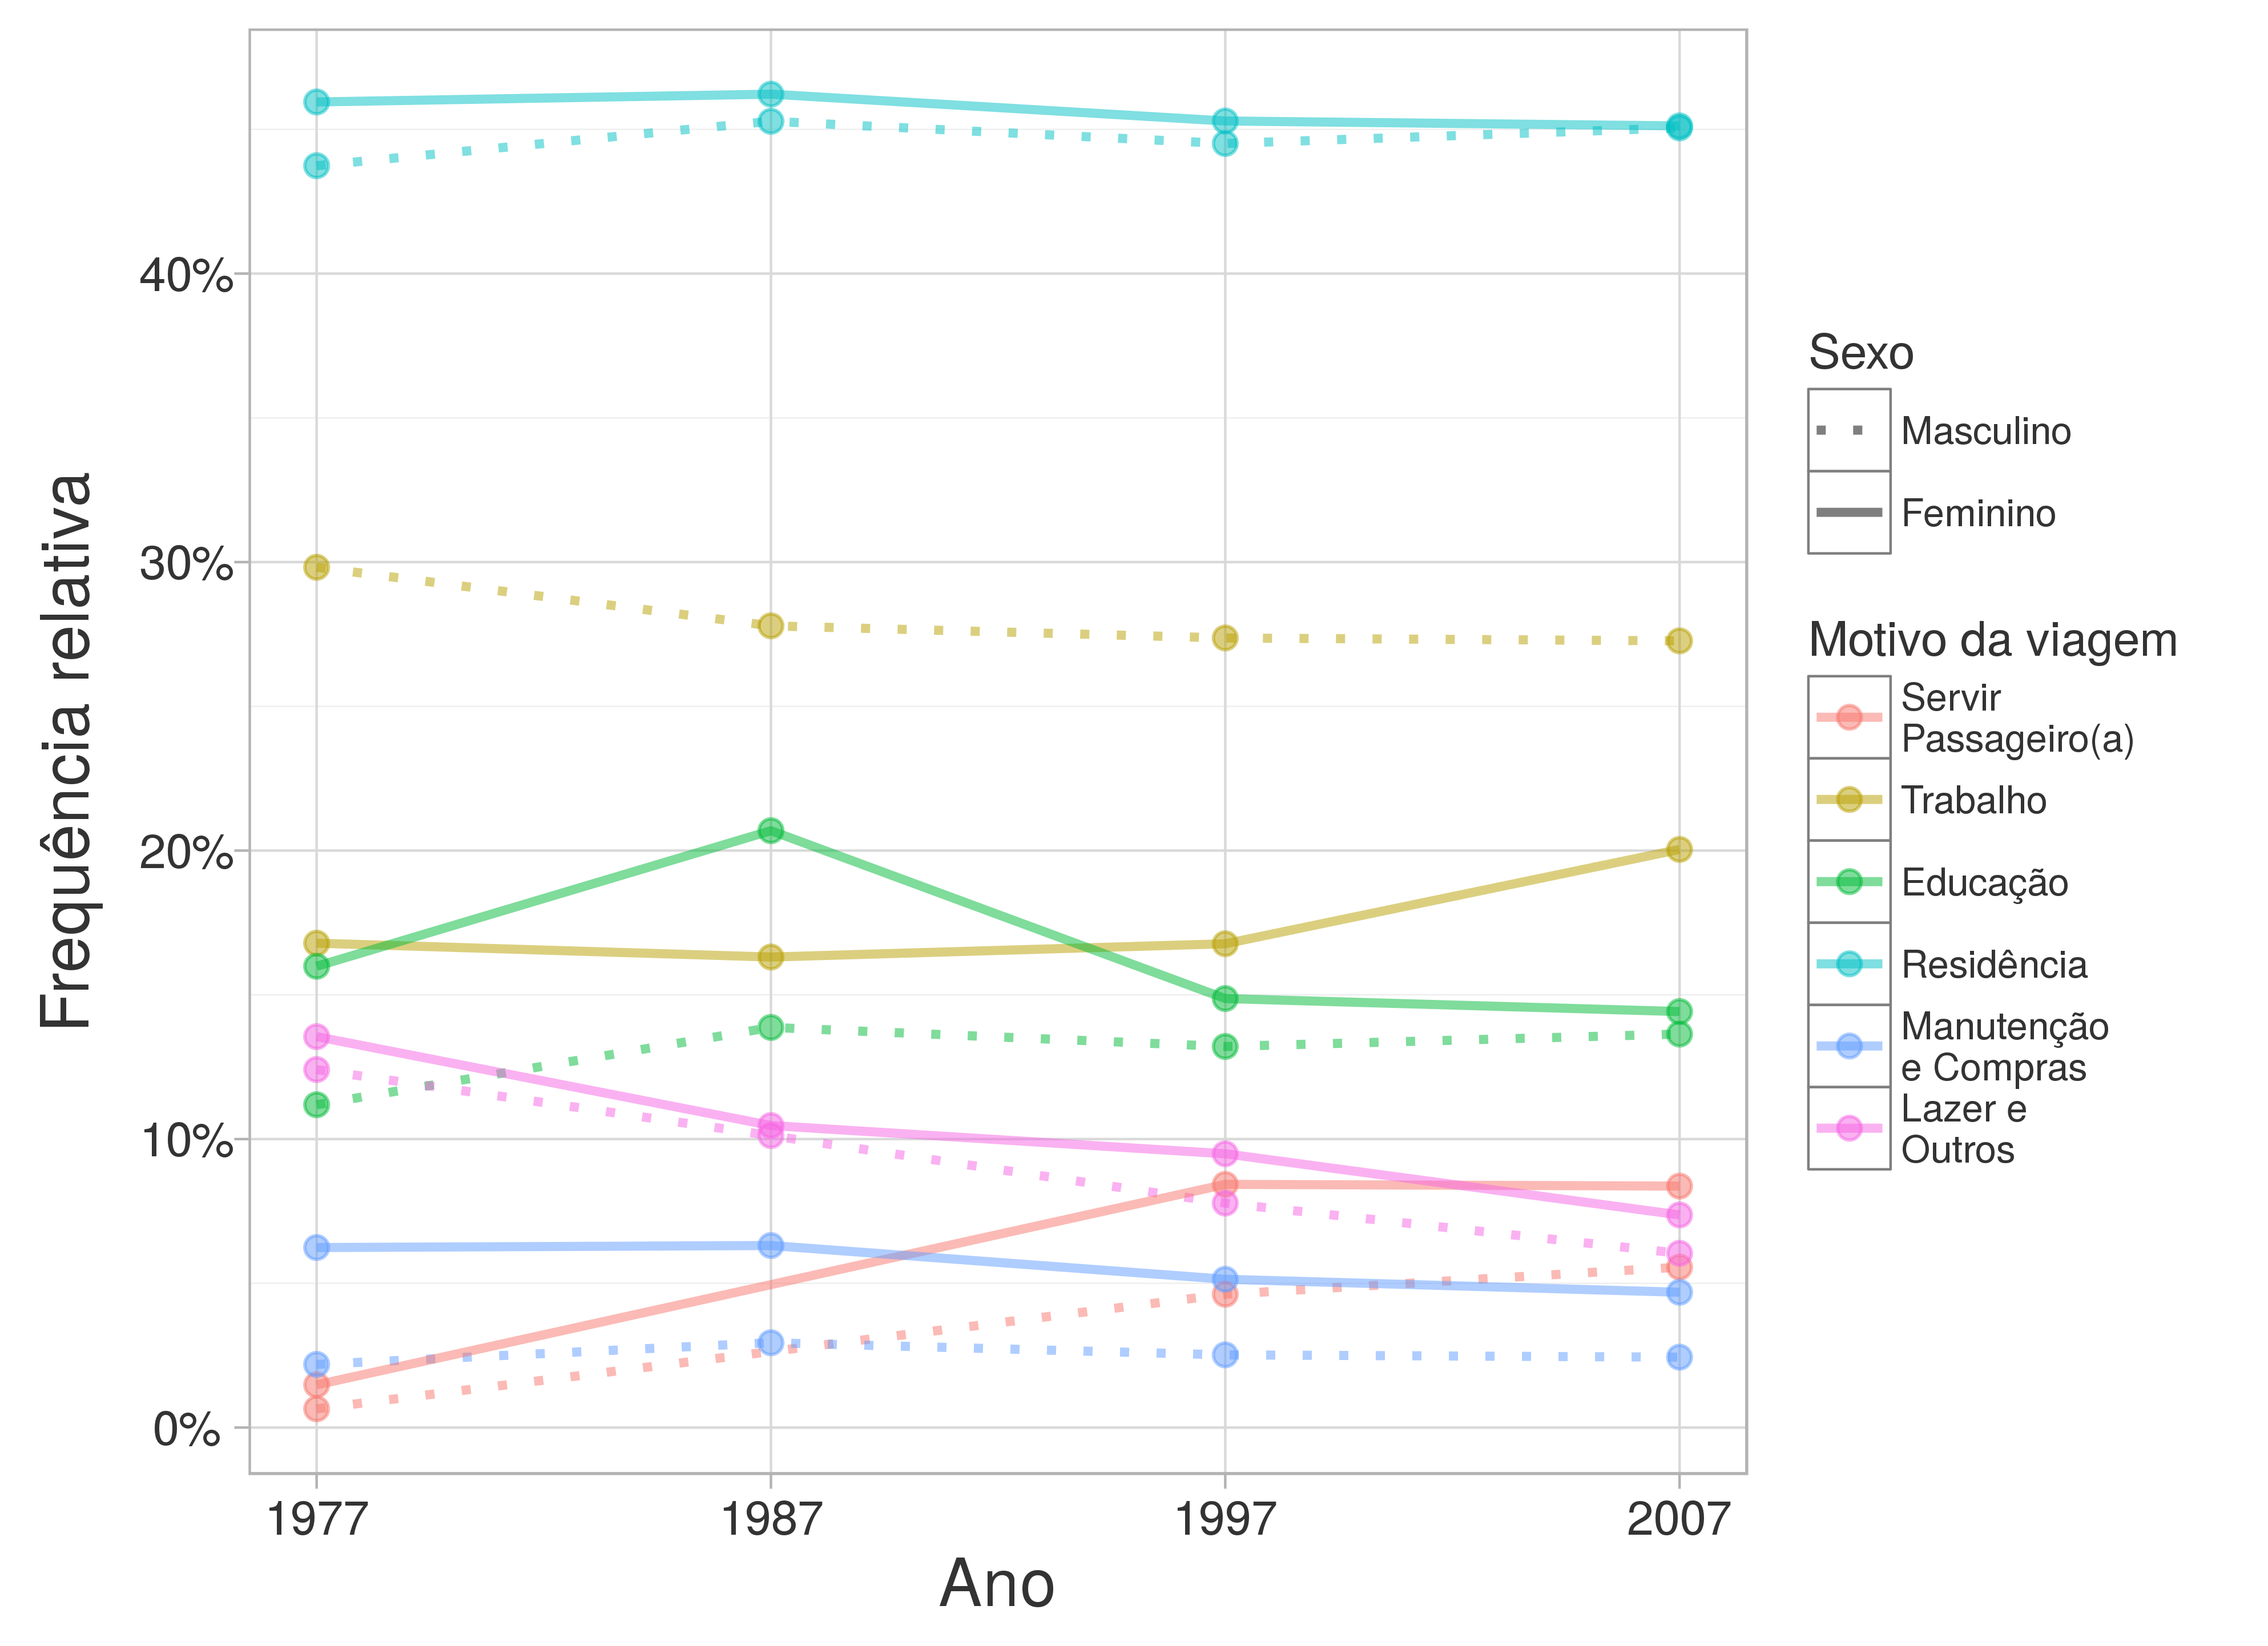
\includegraphics[width=0.9\textwidth]{./imagens/freq-motivo.png}%
    \end{center}%
%    \fonte{Compilação própria}
\end{grafico}%
% Estatísticas para registros com F_VIAG==1 e SEXO
% Expandido com FE_VIAG

%A variável \textbf{DURACAO} representa a duração total da viagem de uma pessoa, a duração média por pessoa é o somatório das durações dividido pelo número total de viagens de cada pessoa.
%Não existem \textit{missing values} neste campo, os valores mínimos para todos anos e ambos sexo são 0, bem como também são 0 os valores do primeiro quartil (25\%). Os valores das demais estatísticas (considerando os fatores de expansão para a população) estão apresentados na Tabela \ref{tab:estat-dur-med-viag}. Conforme já era de se esperar, para quem faz viagem no dia da pesquisa (número de viagem é não nulo) existe a predominância do valor 2, ou seja, são pessoas que saem de suas residências com um propósito único (trabalhar, estudar, fazer compras) e depois retornam à residência após a atividade.
%Percebe-se que, independente do sexo, o número médio de viagens por pessoa em relação a 1977 caiu um pouco em 1987 e 1997 (de 1,67 para 1,64) e subiu novamente em 2007 (para 1,70). Os desvios padrão caíram ao longo do tempo, indicando tendência de menor dispersão dos dados. Os valores de assimetria são positivos, indicando maior concentração à esquerda e cauda longa à direita da distribuição. Os valores de curtose evidenciam não tratar-se de distribuição normal.
%Analisando esses dados segmentados por sexo, vê-se que as medianas são iguais. O número médio e máximo de viagens para mulheres é sempre inferior ao dos homens, para o mesmo ano. Os valores de assimetria para o sexo feminino e o masculino são positivos e convergem para o valor geral com o passar das décadas. 
%A diferença entre o número médio de viagens de mulheres e homens vem diminuindo.

%\begin{table}[htb]
%\centering
%   \IBGEtab{%\renewcommand{\arraystretch}{1.5}%%\ABNTEXfontereduzida%
%        \renewcommand{\arraystretch}{1.5}
%        \caption{Estatísticas da variável ``PESS_DURACAO_MED'', por ano e por sexo}
%        \label{tab:estat-dur-med-viag}
%    }{%
%
%    \begin{tabular}{ccccccc}
%        \toprule
%        \textbf{Geral} & \multicolumn{3}{c}{\textbf{}} & \multicolumn{3}{c}{\textbf{}} \\ \hline
%        \textbf{ANO}   & \textbf{Média} & \textbf{Desvio Padrão} & \textbf{Mediana} & \textbf{Máximo} & \textbf{Assimetria} & \textbf{Curtose} \\ \midrule \midrule
%        \textbf{1977}  & 21,31 & 28,96 & 10,00 & 240 & 2,06 & 5,74 \\ \hline
%        \textbf{1987}  & 22,41 & 30,04 & 10,00 & 360 & 1,95 & 4,68 \\ \hline
%        \textbf{1997}  & 23,22 & 31,07 & 12,50 & 315 & 1,99 & 4,75 \\ \hline
%        \textbf{2007}  & 29,16 & 35,94 & 16,25 & 240 & 1,68 & 2,94 \\\bottomrule          
%
%        \textbf{Sexo Feminino} & \multicolumn{3}{c}{\textbf{}} & \multicolumn{3}{c}{\textbf{}} \\ \hline
%        \textbf{ANO}   & \textbf{Média} & \textbf{Desvio Padrão} & \textbf{Mediana} & \textbf{Máximo} & \textbf{Assimetria} & \textbf{Curtose} \\ \midrule \midrule
%        \textbf{1977}  & 16,49 & 25,70 &  5,00 & 240 & 1,80 & 4,41 \\ \hline
%        \textbf{1987}  & 17,55 & 26,68 &  5,00 & 360 & 1,66 & 3,16 \\ \hline
%        \textbf{1997}  & 19,89 & 28,67 & 10,00 & 300 & 1,82 & 3,93 \\ \hline
%        \textbf{2007}  & 26,49 & 34,93 & 15,00 & 240 & 1,55 & 2,45 \\\bottomrule
%        
%        \textbf{Sexo Masculino} & \multicolumn{3}{c}{\textbf{}} & \multicolumn{3}{c}{\textbf{}} \\ \hline
%        \textbf{ANO}   & \textbf{Média} & \textbf{Desvio Padrão} & \textbf{Mediana} & \textbf{Máximo} & \textbf{Assimetria} & \textbf{Curtose} \\ \midrule \midrule
%        \textbf{1977}  & 26,39 & 31,24 & 16,67 & 240 & 2,41 & 7,94 \\ \hline
%        \textbf{1987}  & 26,80 & 32,49 & 16,67 & 310 & 2,32 & 7,22 \\ \hline
%        \textbf{1997}  & 27,66 & 33,09 & 15,00 & 315 & 2,17 & 5,71 \\ \hline
%        \textbf{2007}  & 32,13 & 36,81 & 20,00 & 240 & 1,82 & 3,54 \\\bottomrule             
%       
%    \end{tabular}
%    }{%
%%		\fonte{Elaboração própria}
%	}
%\end{table}
%% Estatísticas para registros com F_PESS==1, filtro por SEXO
%% Expandido com FE_PESS
%
%\begin{table}[htb]
%\centering
%   \IBGEtab{%\renewcommand{\arraystretch}{1.5}%%\ABNTEXfontereduzida%
%        \renewcommand{\arraystretch}{1.5}
%        \caption{Estatísticas da variável ``PESS_DURACAO_MED'', por ano e por sexo, considerando somente quem fez viagem com duração superior a 4 minutos}
%        \label{tab:estat-dur-med-viag-maisde4}
%    }{%
%
%    \begin{tabular}{ccccccc}
%        \toprule
%        \textbf{Geral} & \multicolumn{3}{c}{\textbf{}} & \multicolumn{3}{c}{\textbf{}} \\ \hline
%        \textbf{ANO}   & \textbf{Média} & \textbf{Desvio Padrão} & \textbf{Mediana} & \textbf{Máximo} & \textbf{Assimetria} & \textbf{Curtose} \\ \midrule \midrule
%        \textbf{1977}  & 35,50 & 29,92 & 27,50 & 240 & 1,83 & 4,76 \\ \hline
%        \textbf{1987}  & 36,00 & 31,02 & 26,25 & 360 & 1,67 & 3,58 \\ \hline
%        \textbf{1997}  & 36,90 & 32,11 & 26,67 & 315 & 1,73 & 3,57 \\ \hline
%        \textbf{2007}  & 43,05 & 36,20 & 30,00 & 240 & 1,47 & 2,16 \\\bottomrule          
%
%        \textbf{Sexo Feminino} & \multicolumn{3}{c}{\textbf{}} & \multicolumn{3}{c}{\textbf{}} \\ \hline
%        \textbf{ANO}   & \textbf{Média} & \textbf{Desvio Padrão} & \textbf{Mediana} & \textbf{Máximo} & \textbf{Assimetria} & \textbf{Curtose} \\ \midrule \midrule
%        \textbf{1977}  & 32,39 & 28,00 & 23,33 & 235 & 1,97 & 5,64 \\ \hline
%        \textbf{1987}  & 33,48 & 28,88 & 22,50 & 360 & 1,88 & 5,10 \\ \hline
%        \textbf{1997}  & 34,48 & 30,39 & 25,00 & 300 & 1,82 & 3,90 \\ \hline
%        \textbf{2007}  & 41,79 & 35,87 & 30,00 & 240 & 1,53 & 2,37 \\\bottomrule
%        
%        \textbf{Sexo Masculino} & \multicolumn{3}{c}{\textbf{}} & \multicolumn{3}{c}{\textbf{}} \\ \hline
%        \textbf{ANO}   & \textbf{Média} & \textbf{Desvio Padrão} & \textbf{Mediana} & \textbf{Máximo} & \textbf{Assimetria} & \textbf{Curtose} \\ \midrule \midrule
%        \textbf{1977}  & 37,89 & 31,10 & 30,00 & 240 & 1,73 & 4,22 \\ \hline
%        \textbf{1987}  & 38,89 & 32,39 & 30,00 & 310 & 1,52 & 2,71 \\ \hline
%        \textbf{1997}  & 39,10 & 33,44 & 30,00 & 315 & 1,65 & 3,25 \\ \hline
%        \textbf{2007}  & 44,27 & 36,48 & 30,00 & 240 & 1,42 & 1,99 \\\bottomrule             
%       
%    \end{tabular}
%    }{%
%%		\fonte{Elaboração própria}
%	}
%\end{table}
%% Estatísticas para registros com F_PESS==1, filtro por SEXO
%% Expandido com FE_PESS

%\begin{grafico}[htb]%
%    \caption{\label{graf:distr-duracao}Distribuição da variável ``PESS_DURACAO_MED'' por ano e por sexo}%
%    \begin{center}%
%        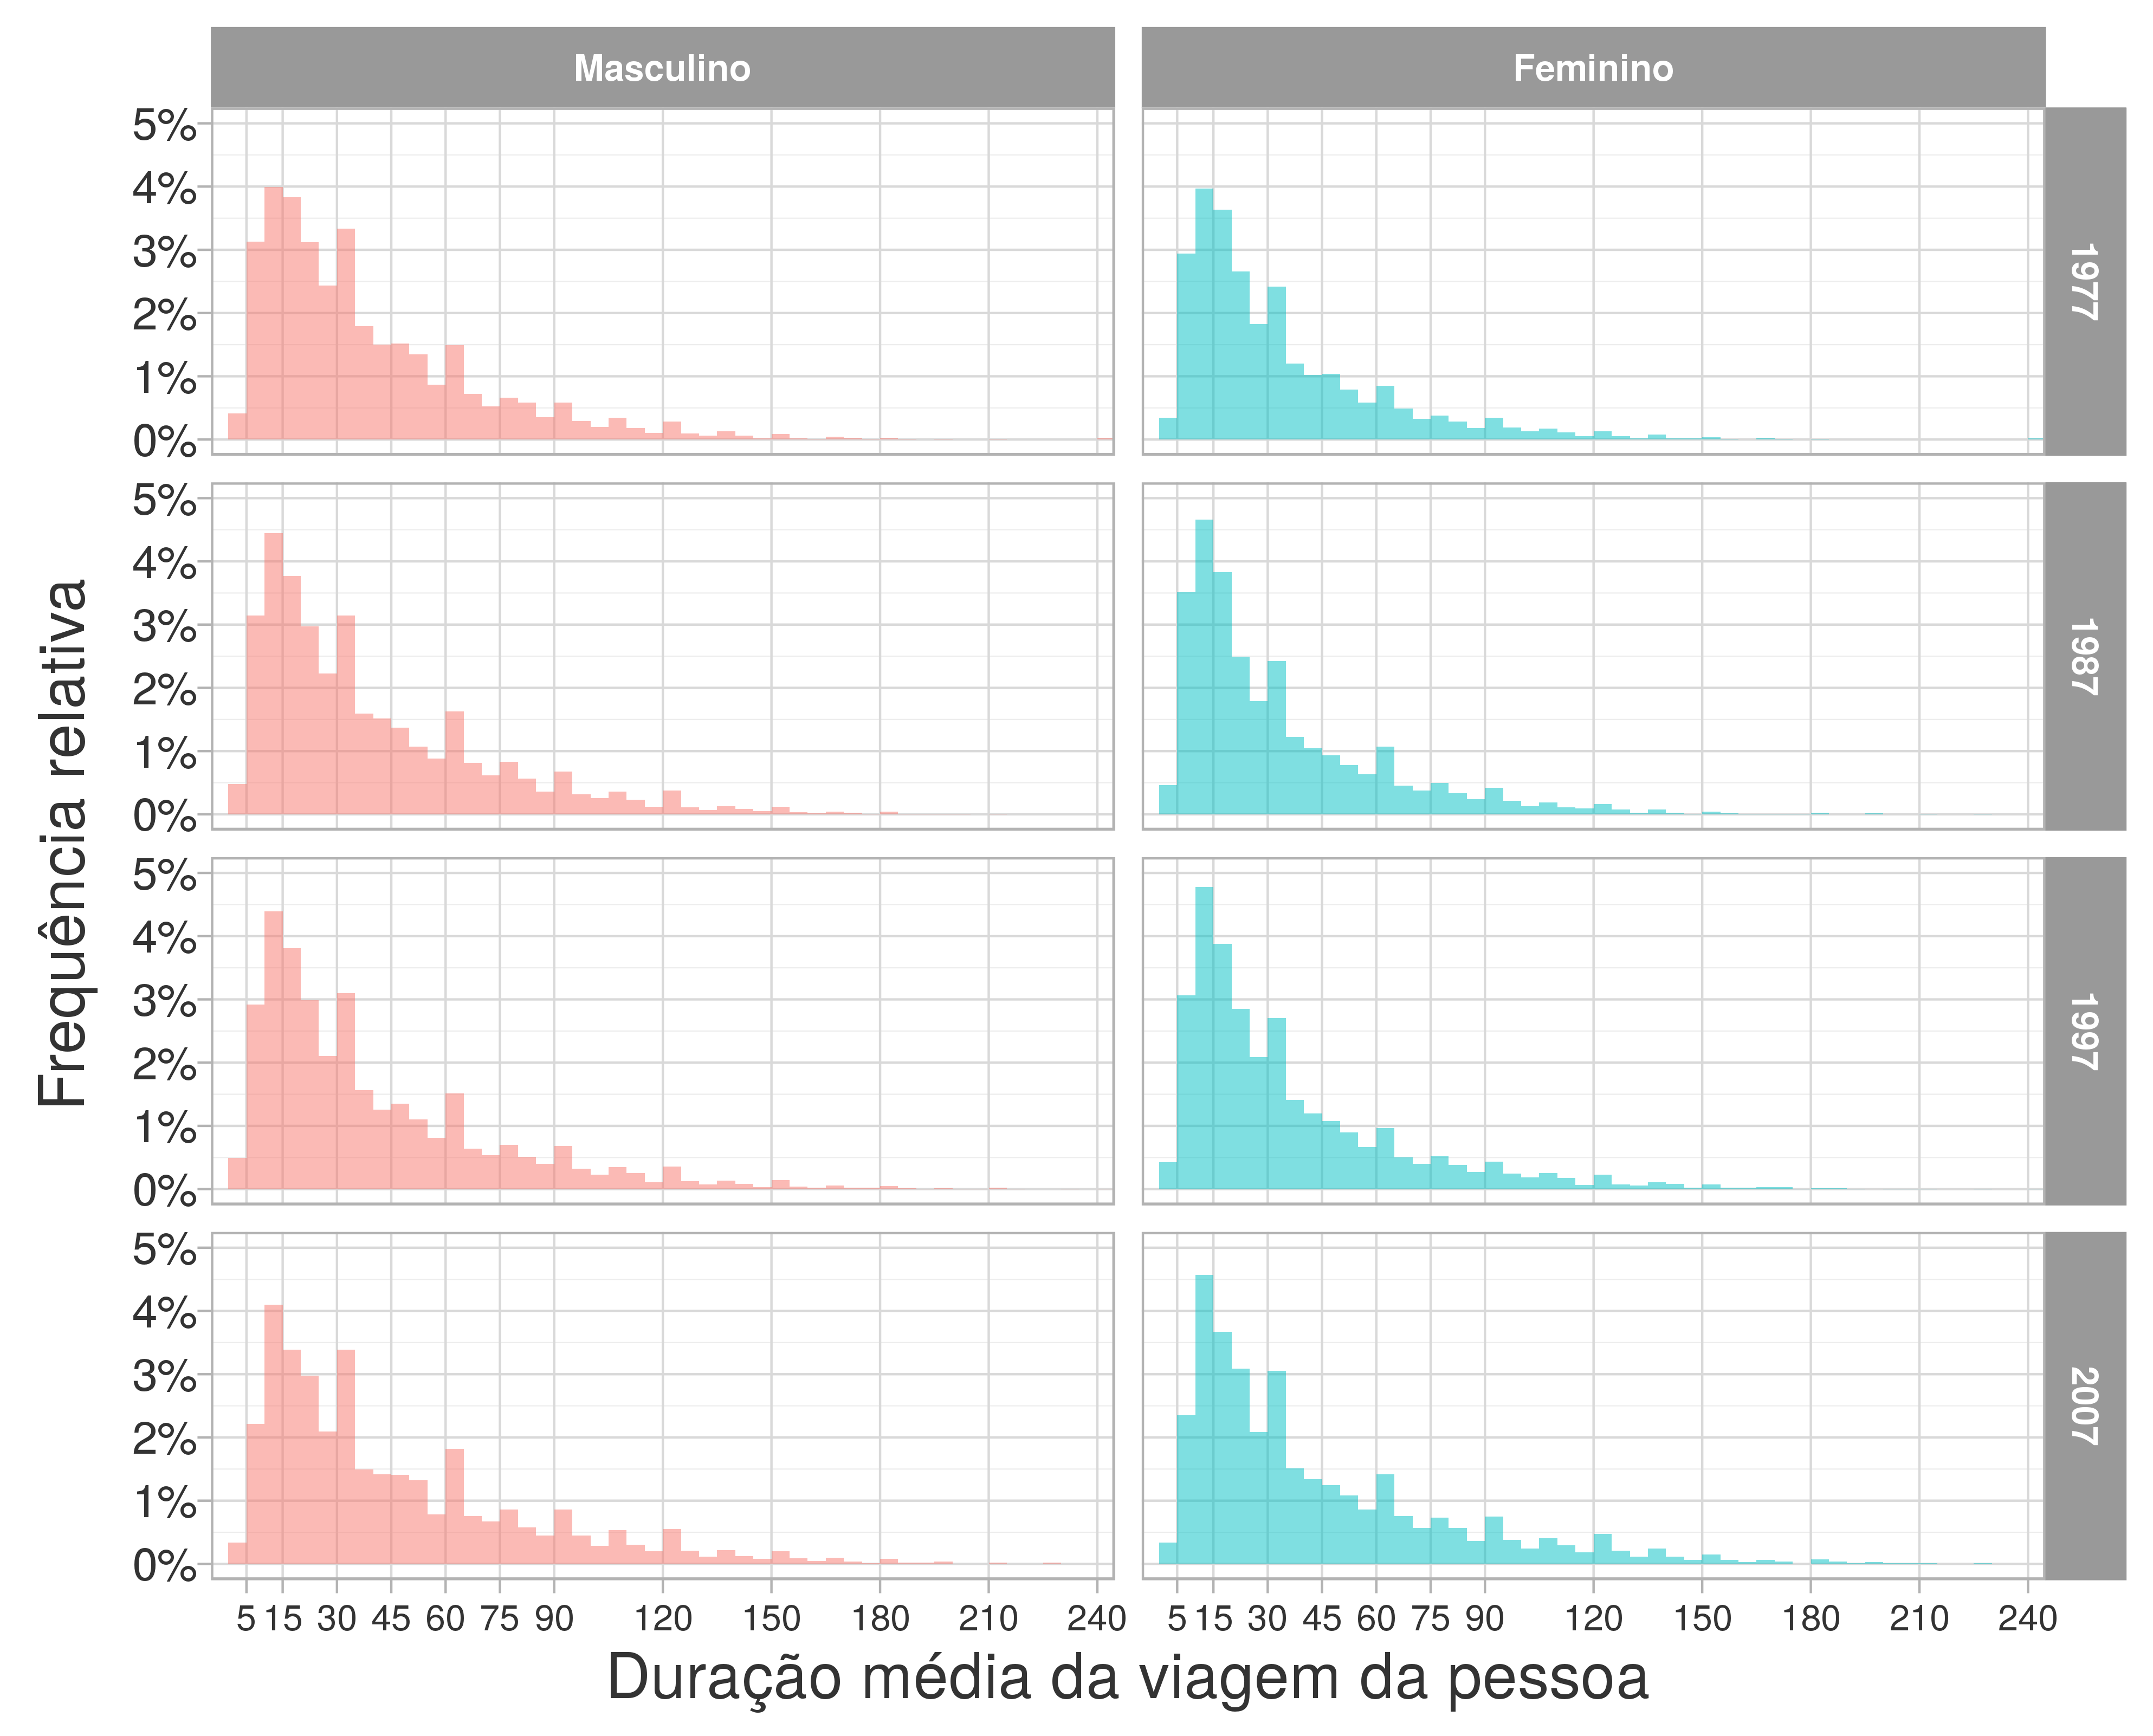
\includegraphics[width=1\textwidth]{./imagens/pess-duracao-med.png}%
%    \end{center}%
%%    \fonte{Compilação própria}
%\end{grafico}%
%% Estatísticas para registros com F_PESS==1 e SEXO
%% Expandido com FE_PESS

%\begin{table}[htb]
%\centering
%   \IBGEtab{%\renewcommand{\arraystretch}{1.5}%%\ABNTEXfontereduzida%
%        \renewcommand{\arraystretch}{1.5}
%        \caption{Estatísticas da variável ``FAM_DURACAO_TOT'', por ano}
%        \label{tab:estat-fam-duracao-tot}
%    }{%
%
%    \begin{tabular}{ccccccc}
%        \toprule
%        \textbf{} & \multicolumn{6}{c}{\textbf{Considerando famílias em que a duração média é superior a 4 minutos}} \\ \hline
%        \textbf{ANO}   & \textbf{Média} & \textbf{Desvio Padrão} & \textbf{Mediana} & \textbf{Máximo} & \textbf{Assimetria} & \textbf{Curtose} \\ \midrule \midrule
%        \textbf{1977}  & 293,14 & 222,68 & 240,00 & 2090 & 1,59 & 3,87 \\ \hline
%        \textbf{1987}  & 265,22 & 199,68 & 220,00 & 2703 & 1,69 & 5,23 \\ \hline
%        \textbf{1997}  & 256,91 & 187,29 & 215,00 & 1890 & 1,42 & 2,87 \\ \hline
%        \textbf{2007}  & 279,18 & 201,34 & 240,00 & 3035 & 1,72 & 9,02 \\\bottomrule          
%
%        \textbf{} & \multicolumn{6}{c}{\textbf{Considerando inclusive família em que ninguém fez viagem}} \\ \hline
%        \textbf{ANO}   & \textbf{Média} & \textbf{Desvio Padrão} & \textbf{Mediana} & \textbf{Máximo} & \textbf{Assimetria} & \textbf{Curtose} \\ \midrule \midrule
%        \textbf{1977}  & 270,74 & 220,08 & 220,00 & 2090 & 1,55 & 3,86 \\ \hline
%        \textbf{1987}  & 251,07 & 200,59 & 210,00 & 2703 & 1,68 & 5,71 \\ \hline
%        \textbf{1997}  & 240,13 & 193,64 & 200,00 & 1890 & 1,37 & 2,87 \\ \hline
%        \textbf{2007}  & 242,07 & 194,09 & 205,00 & 3035 & 1,58 & 7,25 \\\bottomrule
%
%    \end{tabular}
%    }{%
%%		\fonte{Elaboração própria}
%	}
%\end{table}
%% Estatísticas para registros com F_FAM==1, filtro por ANO
%% Expandido com FE_FAM

%O Gráfico \ref{graf:distr-dur-viag} foi construído considerando-se apenas as viagens cuja duração fosse igual ou superior a 5 minutos. Em todos os anos, para homens e para mulheres, percebem-se alguns picos que ocorrem nos valores múltiplos de cinco minutos. Isso porque a duração de viagem é aquela percebida e declarada pelo(a) respondente. Em 1977, a duração das viagens mais curtas (como 5 e 30 minutos) era menos frequente entre as mulheres (13\% e 14\%, respectivamente) do que entre os homens (26\% e 15\%). Em 1987 as viagens de 5 minutos passam a ser mais frequentes entre mulheres (32\%) do que entre homens (26,5\%). Essa situação se inverte em 1997 e retorna em 2007.
%Em todos os anos as viagens mais longas (de 60 e 90 minutos) são mais frequentes entre os homens do que entre as mulheres.
%Na Tabela \ref{tab:dur-med-viag} são apresentadas as durações médias de viagens para homens e mulheres. As médias de homens são superiores às das mulheres, ao nível de significância estatística de 5\%. É possível perceber que a duração média de viagem para ambos vem crescendo e a diferença entre esses grupos vem diminuindo.


A variável \textbf{DURACAO} tem suas principais estatísticas apresentadas na Tabela \ref{tab:estat-duracao}.
Não existem \textit{missing values} neste campo e, desconsiderando quem não fez viagem (duração igual a 0 minutos), os valores mínimos para todos anos e ambos sexo são 1 minuto.
As medianas da duração, independente do sexo, saem de 30 minutos em 1977 para 20 minutos em 1987 e 1997 e retornam para o valor 30 em 2007.
Os valores de assimetria são todos positivos, indicando maior concentração à esquerda e cauda longa à direita da distribuição.
Os valores de curtose evidenciam não se tratar de distribuição normal.
O tempo médio geral de viagem vai de 1977 para 1987 e daí em diante só aumenta, comportamento semelhante ao segmento feminino.
Os tempos médios das viagens do homens cresce sistematicamente década a década, da ordem de 1 minuto entre 1977, 1987 e 1997. Já 2007 o acréscimo no tempo médio de viagem masculino subiu 4,5 minutos - tal efeito pode ser explicado pela expansão urbana da RMSP.
Analisando esses dados segmentados por sexo, vê-se que as medianas das mulheres são sempre 5 minutos a menos que as dos homens. 
A diferença entre as durações médias das viagens de mulheres e de homens cresce de quase 0,5 minuto em 1977 para pouco mais de 5,5 minutos em 1987 e vem diminuindo desde então.
Foram feitos teste t para avaliar se eram estatisticamente significantes (intervalo de confiança de 95\%) as médias entre os sexos, no mesmo ano; e entre os anos, para o mesmo sexo. Todas médias foram estatisticamente diferentes umas das outras.

\begin{table}[htb]
\centering
   \IBGEtab{%\renewcommand{\arraystretch}{1.5}%%\ABNTEXfontereduzida%
        \renewcommand{\arraystretch}{1.5}
        \caption{Estatísticas da variável ``DURACAO'', por ano}
        \label{tab:estat-duracao}
    }{%

    \begin{tabular}{ccccccc}
        \toprule
        \textbf{Total} & \multicolumn{6}{c}{\textbf{}} \\ \hline
        \textbf{ANO}   & \textbf{Média} & \textbf{Desvio Padrão} & \textbf{Mediana} & \textbf{Máximo} & \textbf{Assimetria} & \textbf{Curtose} \\ \midrule \midrule
        \textbf{1977}  & 36,07 & 31,99 & 30 & 240 & 1,74 & 3,78 \\ \hline
        \textbf{1987}  & 33,27 & 31,99 & 20 & 360 & 1,92 & 4,97 \\ \hline
        \textbf{1997}  & 34,13 & 33,52 & 20 & 370 & 1,94 & 4,54 \\ \hline
        \textbf{2007}  & 39,29 & 37,22 & 30 & 299 & 1,74 & 3,37 \\\bottomrule          

        \textbf{Sexo feminino} & \multicolumn{6}{c}{\textbf{}} \\ \hline
        \textbf{ANO}   & \textbf{Média} & \textbf{Desvio Padrão} & \textbf{Mediana} & \textbf{Máximo} & \textbf{Assimetria} & \textbf{Curtose} \\ \midrule \midrule
        \textbf{1977}  & 34,09 & 30,54 & 25 & 240 & 1,81 & 4,12 \\ \hline
        \textbf{1987}  & 30,15 & 29,76 & 20 & 360 & 2,08 & 5,89 \\ \hline
        \textbf{1997}  & 31,97 & 31,67 & 20 & 315 & 2,02 & 4,78 \\ \hline
        \textbf{2007}  & 37,96 & 36,72 & 25 & 299 & 1,81 & 3,68 \\\bottomrule     

        \textbf{Sexo Masculino} & \multicolumn{6}{c}{\textbf{}} \\ \hline
        \textbf{ANO}   & \textbf{Média} & \textbf{Desvio Padrão} & \textbf{Mediana} & \textbf{Máximo} & \textbf{Assimetria} & \textbf{Curtose} \\ \midrule \midrule
        \textbf{1977}  & 34,47 & 32,89 & 30 & 240 & 1,69 & 3,53 \\ \hline
        \textbf{1987}  & 35,83 & 33,50 & 25 & 360 & 1,80 & 4,36 \\ \hline
        \textbf{1997}  & 36,11 & 35,02 & 25 & 370 & 1,86 & 4,25 \\ \hline
        \textbf{2007}  & 40,61 & 37,67 & 30 & 270 & 1,67 & 3,11 \\\bottomrule             

    \end{tabular}
    }{%
%		\fonte{Elaboração própria}
	}
\end{table}
% Estatísticas para registros com F_FAM==1, filtro por ANO
% Expandido com FE_FAM

Com o intuito de melhor explorar as durações médias das viagens analisando modos e motivos, foram elaborados os Gráficos \ref{graf:duracao-modo}, \ref{graf:duracao-coletivo} e \ref{graf:duracao-motivo}.
O Gráfico \ref{graf:duracao-modo} apresenta as durações médias do transporte coletivo, individual e a pé, para homens e para mulheres. Verifica-se que:
\begin{compactitem}[]
\item (i) As durações médias de homens e mulheres são muito próximas para as viagens a pé, girando em torno de 15 minutos para ambos.
\item (ii) A duração média no transporte individual cai um pouco de 1977 para 1987 (de 23,0 para 20,4 min para mulheres e de 27,07 para 25,7 min para homens).
\item (iii) A duração média no transporte individual aumenta de 1987 para 2007 (7,3 min para mulheres e 8,1 min para homens).
\item (iv) A duração média no transporte coletivo aumenta entre 1977 e 2007 para ambos sexos, sendo a taxa mais acentuada de 1997 para 2007. 
\item (v) As diferenças nas durações médias nas viagens feitas por transporte coletivo entre mulheres e homens aumenta de 1977 (4,2 min) para 1987 (6,3 min) e depois decresce nas décadas seguintes (6,0 min em 1997 e 3,2 min em 2007).
\end{compactitem}

\begin{grafico}[htb]%
    \caption{\label{graf:duracao-modo}Durações médias de viagem por ano e por sexo, segundo os modos (agregados)}%
    \begin{center}%
        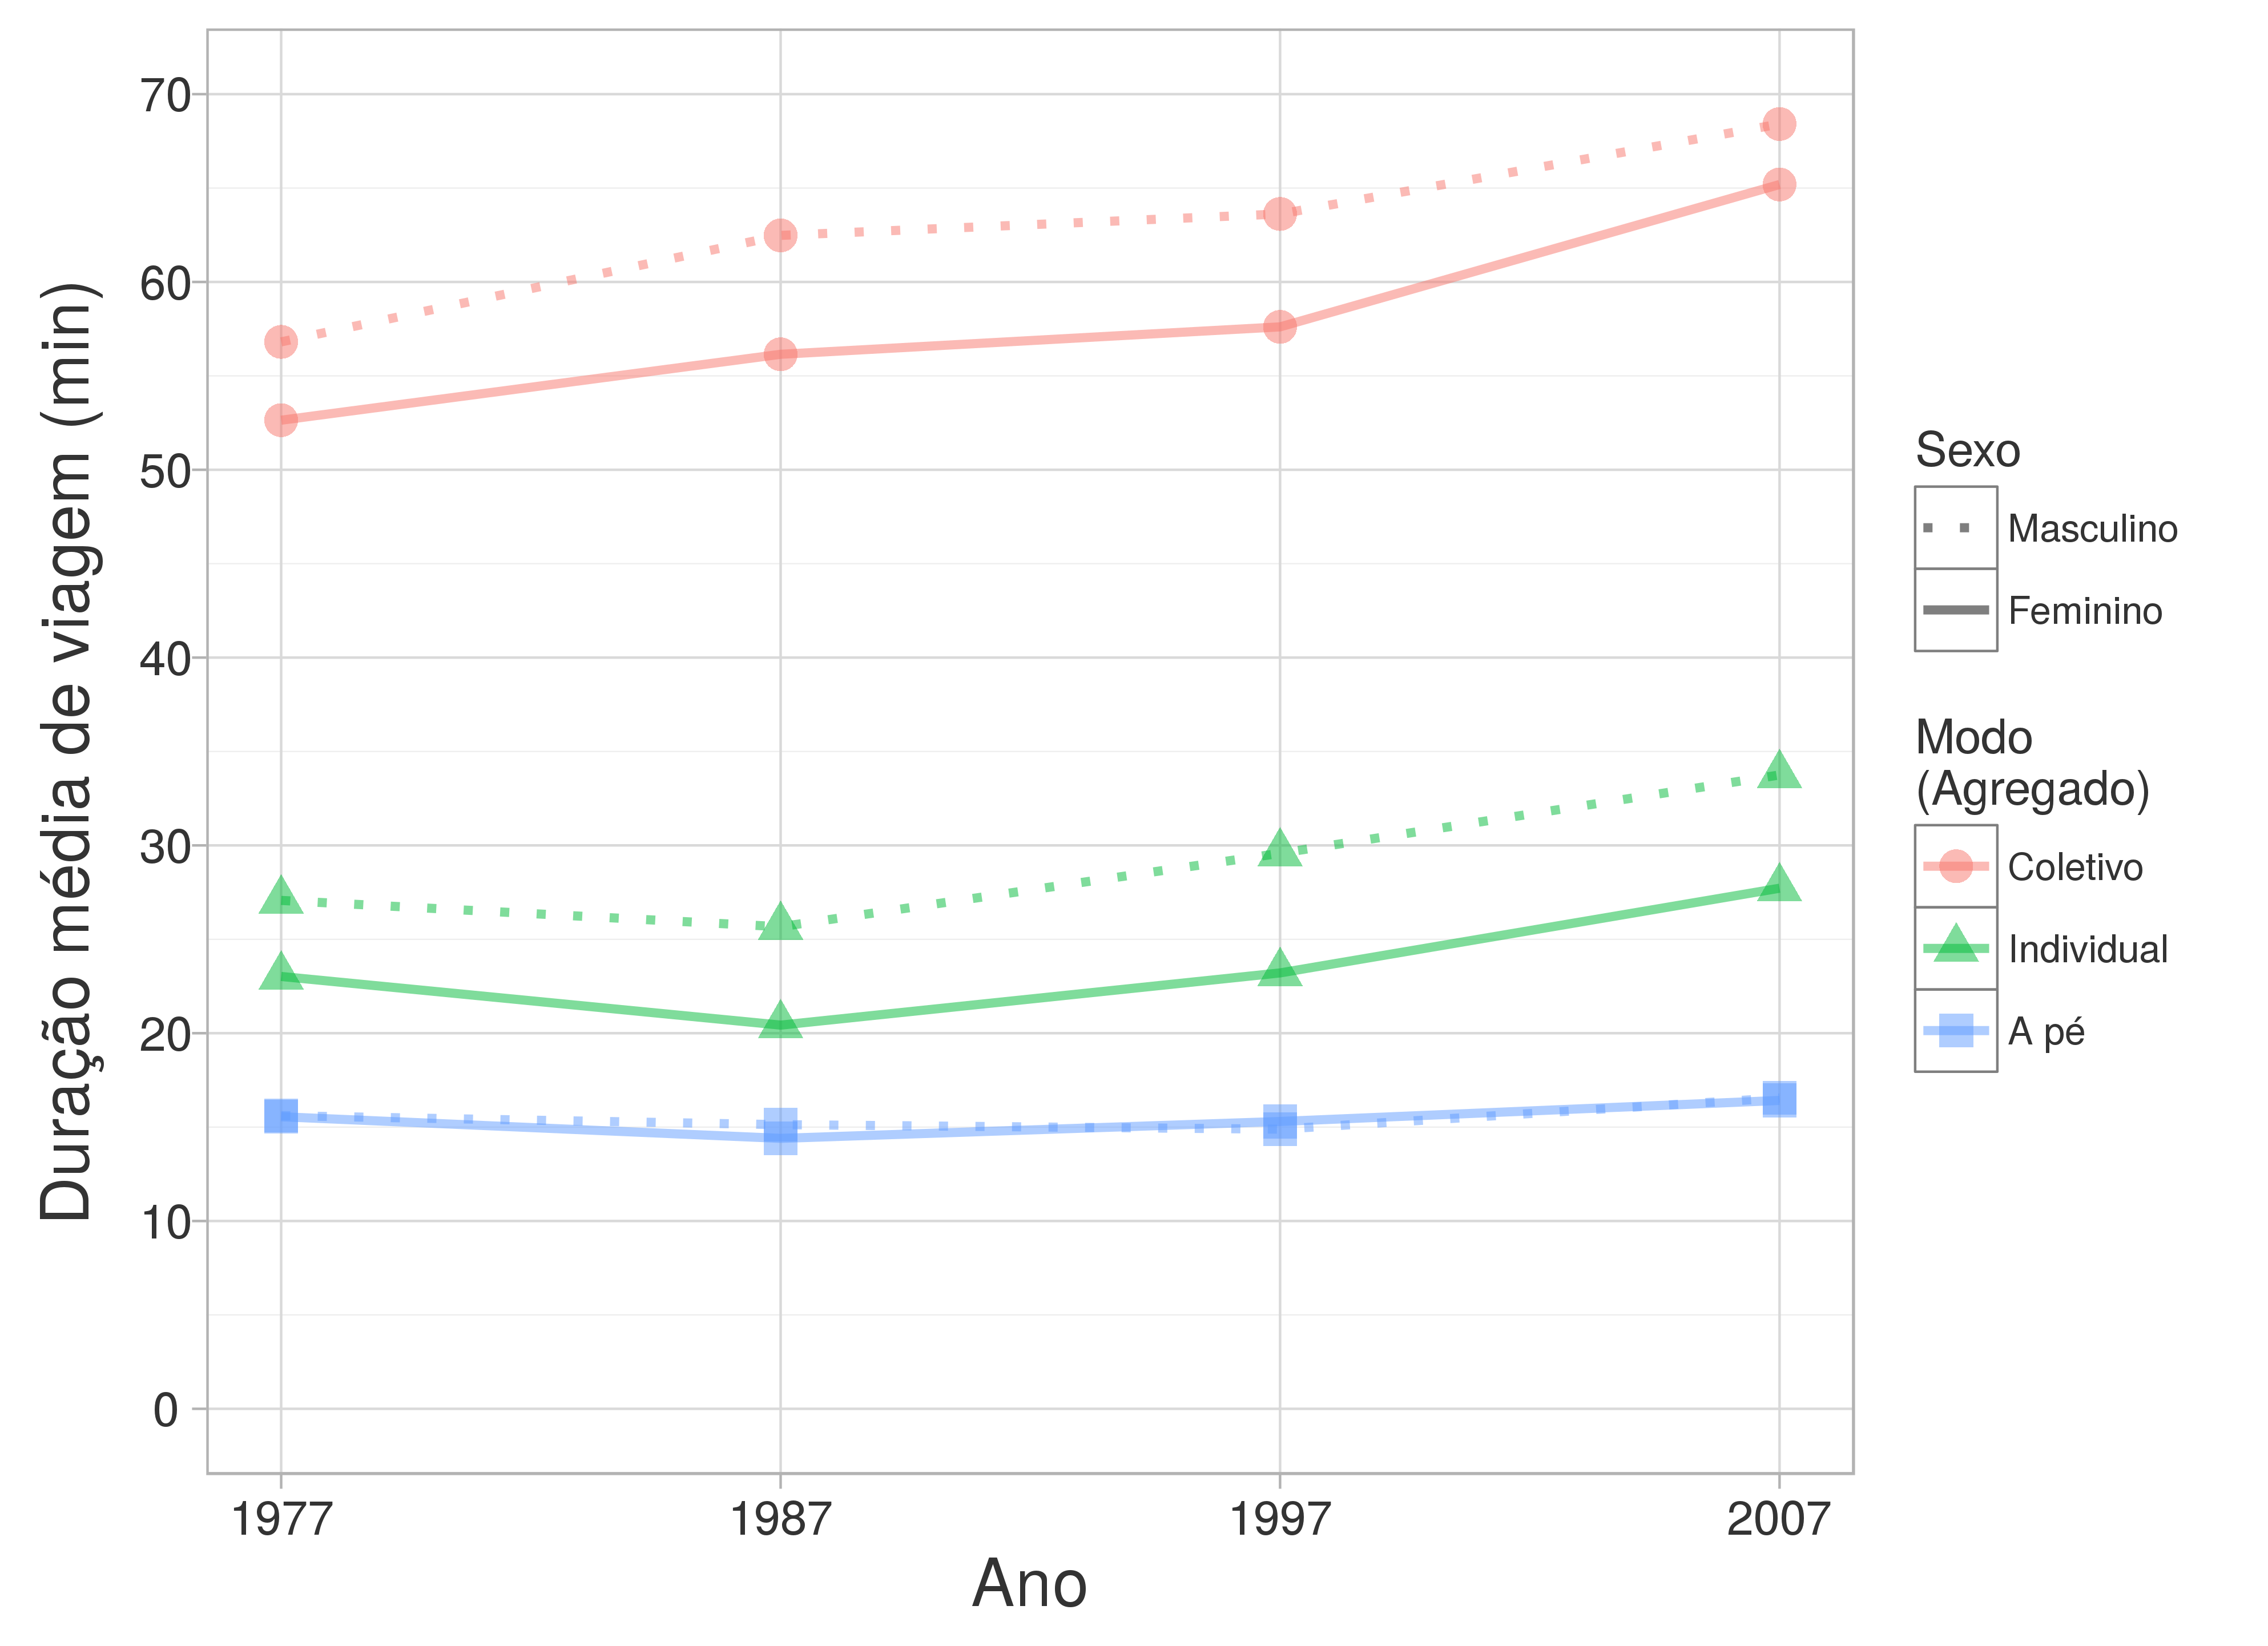
\includegraphics[width=1\textwidth]{./imagens/duracao-modo.png}%
    \end{center}%
%    \fonte{Compilação própria}
\end{grafico}%
% Estatísticas para registros com F_VIAG==1 e SEXO
% Expandido com FE_VIAG

O Gráfico \ref{graf:duracao-coletivo} apresenta as durações médias dos modos de transporte coletivo (ônibus de linha, ônibus de empresa/escolar, lotação/perua/van/microônibus, Metrô e trem), para homens e para mulheres - foram separados os modos de alta capacidade dos demais para facilitar a compreensão dos gráficos. Verifica-se que:
\begin{compactitem}[]
\item (i) A duração média do trem é superior a todos outros modos, inclusive o Metrô, com médias gerais caindo de 83,3 min em 1977 para 80,8 min em 1987 e crescendo para 89,5 min em 1997. Em 2007, esse valor permanece no mesmo patamar de 1997 (91,2 min).
\item (ii) Para o trem, a duração média feminina é inferior à masculina em 1977 (diferença de 2,9 min) e 1987 (diferença de 2,1 min), supera a masculina em 1997 (por 1,5 min) e distancia da masculina em 2007 (diferença de 8,0 min).
\item (iii) A duração média das viagens de Metrô crescem sistematicamente, pelo menos 6 min por década, de 1977 (53,8 min) a 2007 (74,4 min).
\item (iv) Para o Metrô, a duração média feminina é superior à masculina em 1977 (diferença de 1,3 min) e em 2007 (diferença de 1,7 min). A situação é inversa, com durações médias das viagens masculinas superiores às femininas em 1987 (diferença de 3,8 min) e 1997 (diferença de 5,0 min).
\item (v) A duração média das viagens dos ônibus de linha crescem sistematicamente, 5 min entre 1977 e 1987, 0,9 min entre 1987 e 1997, e 8,8 min entre 1997 e 2007.
\item (vi) Para ônibus de linha, a duração média feminina é inferior à masculina - a diferença é de 4,0 min em 1977, de 6,9 min em 1987, de 6,3 min em 1997 e de 3,9 min em 2007.
\item (vii) A duração média das viagens de lotações/vans crescem de 1977 (54,1 min) para 1987 (60,8 min), caem em 1997 (49,9 min) e sobem novamente em 2007 (66,3 min).
\item (viii) Para viagens de lotações/vans, a duração média feminina era inferior à masculina em 1977 (diferença de 6,4 min) e em 2007 (diferença 9,4 de min). A situação é inversa em 1987, com diferenças de 7,7 min entre os sexos. E, em 1997, as durações médias são estatisticamente iguais.
\item (ix) A duração média das viagens de ônibus escolar/fretado são as menores entre os transportes coletivos, para ambos sexos variando numa faixa de 40,9 a 44,2 min.
\item (x) Para viagens de ônibus escolar/fretado, a duração média feminina é sempre inferior à masculina - a diferença é de 6,8 min em 1977, de 7,2 min em 1987, de 7,1 min em 1997 e de 2,9 min em 2007.
\end{compactitem}

\begin{grafico}[htb]%
    \caption{\label{graf:duracao-coletivo}Durações médias de viagem por ano e por sexo, segundo os modos coletivos}%
    \begin{center}%
        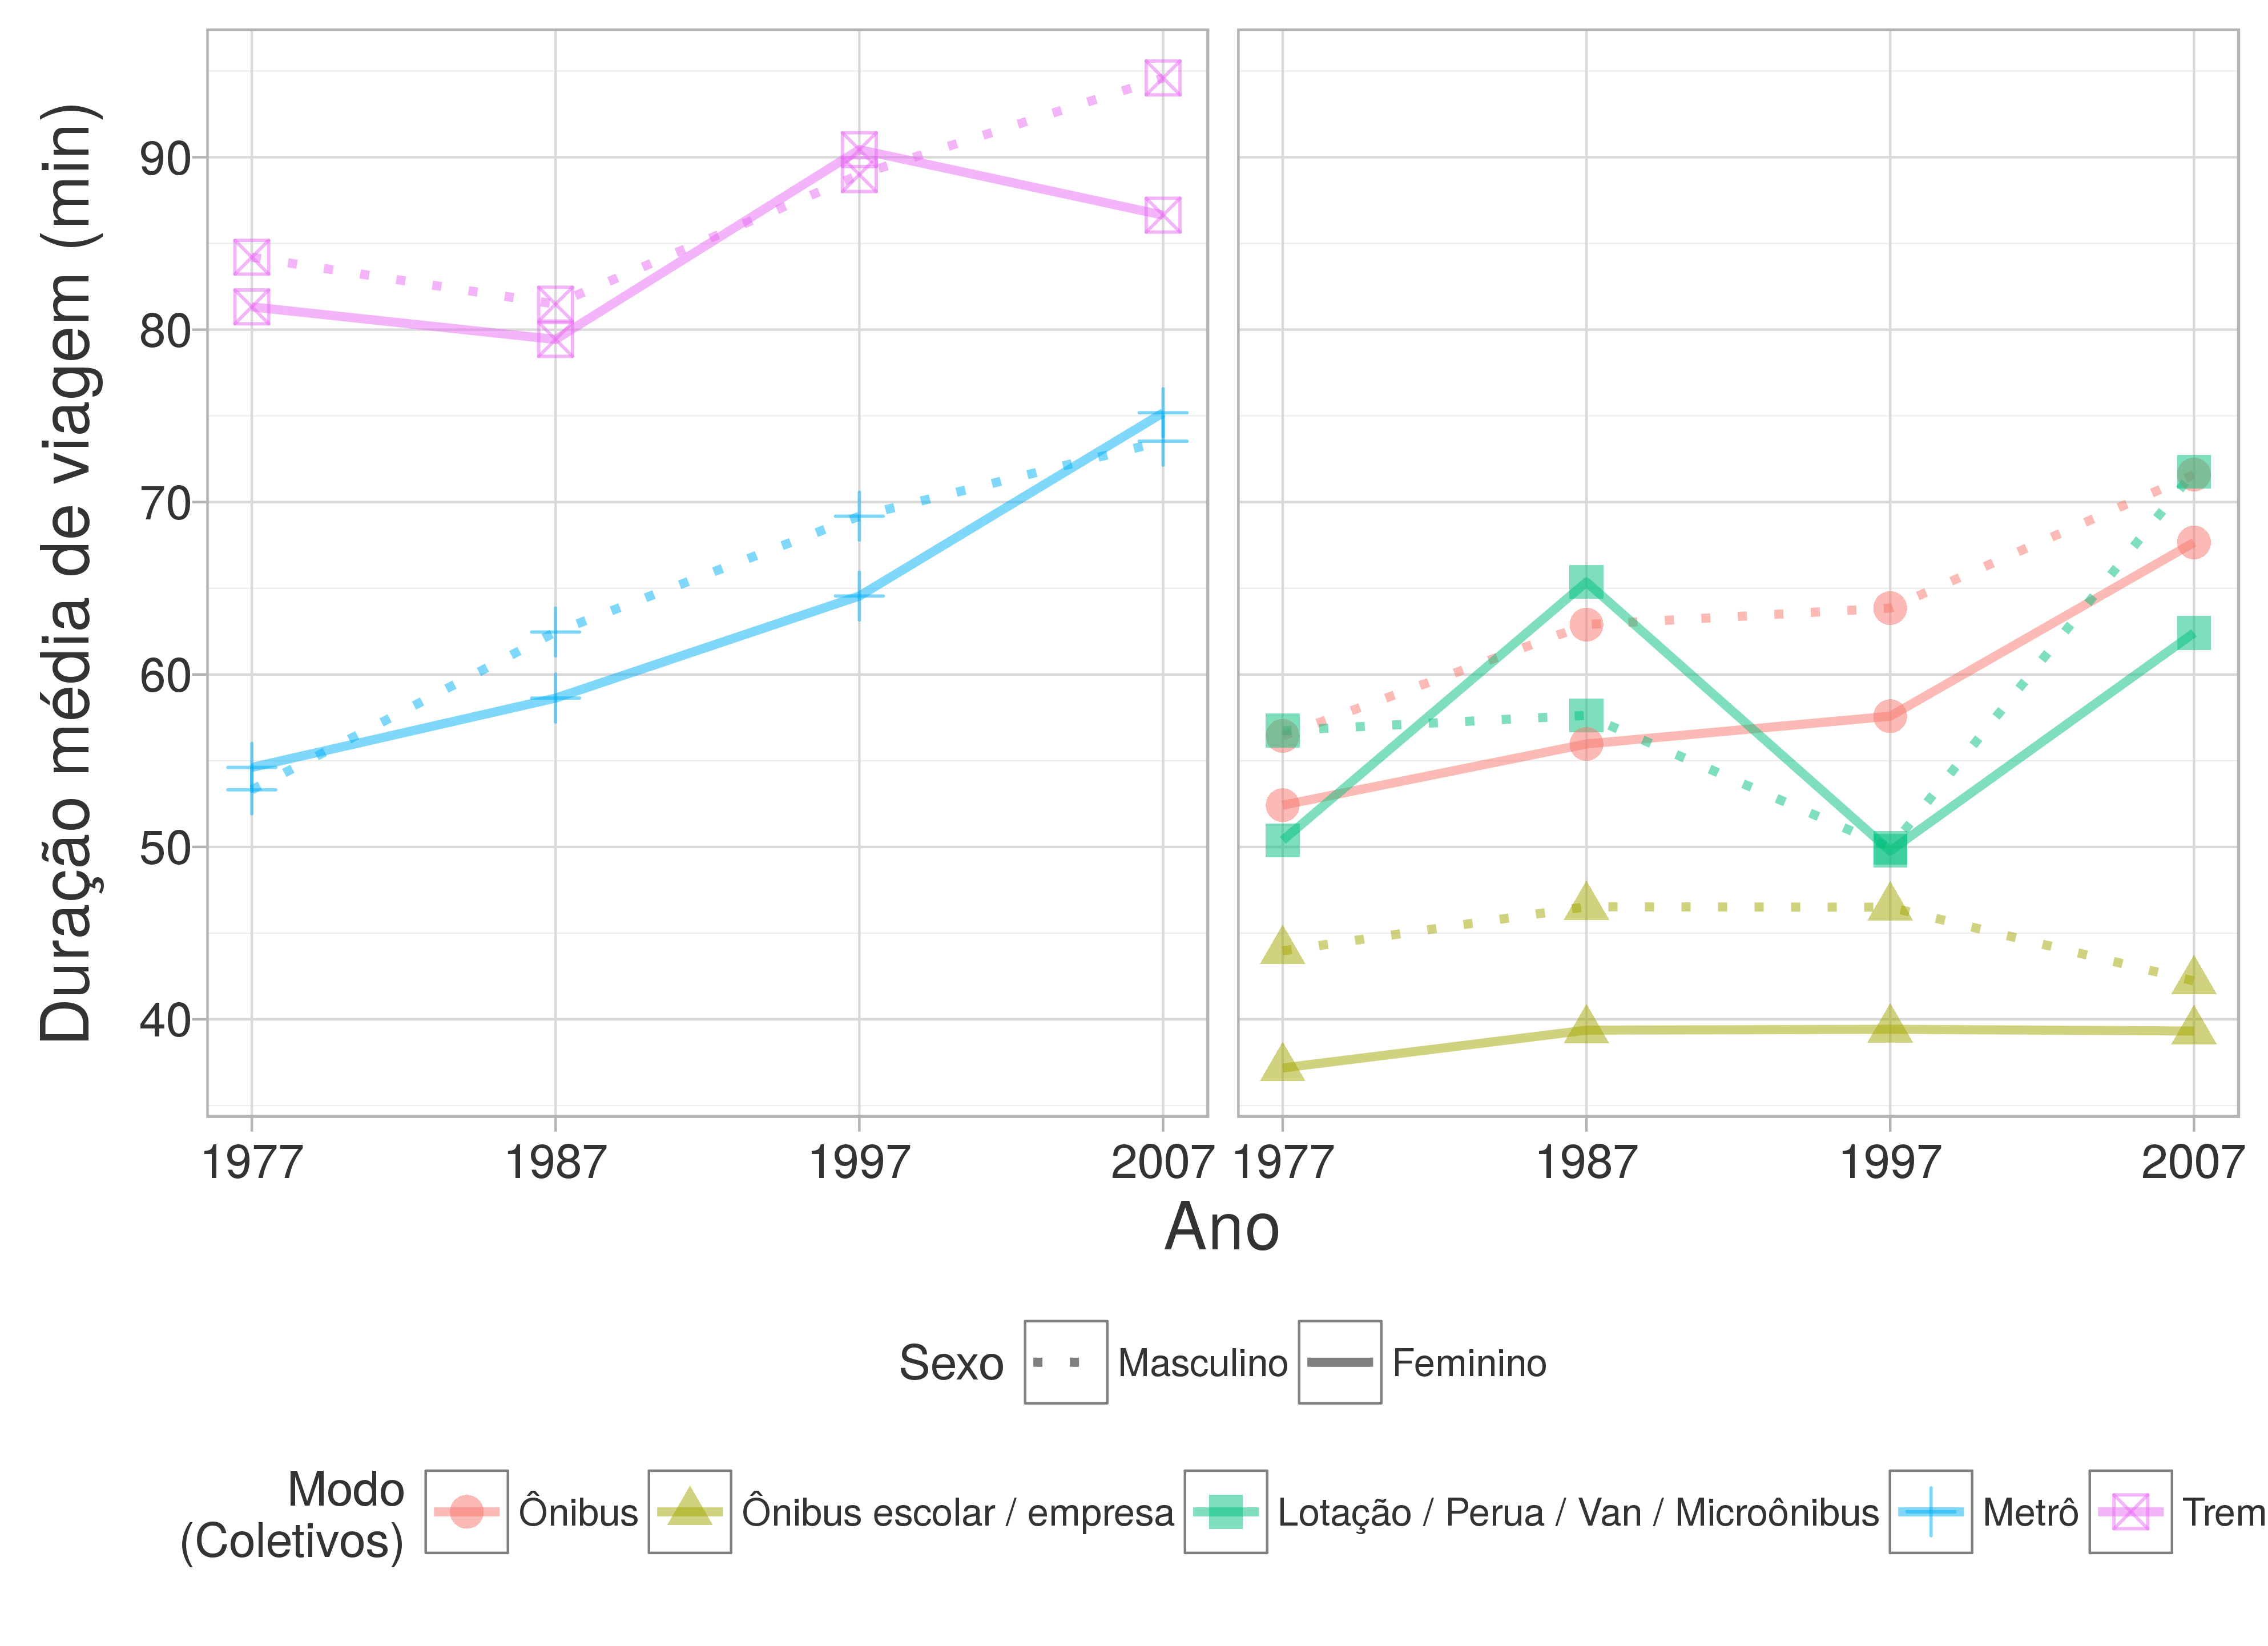
\includegraphics[width=1\textwidth]{./imagens/duracao-coletivo.png}%
    \end{center}%
%    \fonte{Compilação própria}
\end{grafico}%
% Estatísticas para registros com F_VIAG==1 e SEXO
% Expandido com FE_VIAG

O Gráfico \ref{graf:duracao-motivo} apresenta as durações médias por motivo de viagem (trabalho, educação, servir passageiro, manutenção/compras e lazer/outros), para homens e para mulheres. Verifica-se que:
\begin{compactitem}[]
\item (i) A duração média da viagem motivo trabalho (de natureza compulsória) é superior a de todos outros motivos. Ela permanece no mesmo patamar entre 1977 (40,9 min) e 1987 (40,8 min), sobe um pouco em 1997 (42,7 min) e continua a subir em 2007 (48,9 min).
\item (ii) Para o motivo trabalho, a duração média feminina é estatisticamente igual à masculina em 1977, inferior, em 1987 (diferença de 2,5 min) e em 1997 (diferenças de 1,3 min) e levemente superior em 2007 (0,7 min).
\item (iii) A duração média das viagens motivo educação decresce de 1977 (20,9 min) para 1987 (18,3 min), a partir de quando sobem até 2007 (26,1 min).
\item (iv) Para o motivo educação, a duração média feminina é praticamente igual à masculina em 1977 e em 1997 (diferenças de menos de 0,4 min), levemente inferior à masculina em 1987 (diferença de 0,9 min) e superior em 2007 (diferença de 0,6 min).
\item (v) A duração média das viagens motivo manutenção/compras decresce de 1977 (35,2 min) para 1987 (33,9 min), a partir de quando sobem até 2007 (38,0 min).
\item (vi) Para viagens motivo manutenção/compras, a duração média feminina é inferior à masculina - a diferença é de 1,9 min em 1977, de 0,7 min em 1987, de 3,3 min em 1997 e de 0,7 min em 2007.
\item (vii) A duração média das viagens motivo lazer/outros decresce de 1977 (34,3 min) para 1987 (32,9 min), a partir de quando sobem até 2007 (35,6 min).
\item (viii) Para o motivo lazer/outros, a duração média feminina é praticamente igual à masculina em 1997, sendo antes disso inferior à masculina (diferenças de 0,6 e 2,4 min para 1977 e 1987, respectivamente) e depois disso superior à masculina (diferença de 0,9 min em 2007).
\item (ix) A duração média das viagens motivo servir passageiro decresce de 1977 (37,2 min) para 1997 (20,4 min), a partir de quando sobem até 2007 (23,1 min). Vale destacar que em 1987 não havia o modo servir passageiro.
\item (x) Para viagens motivo servir passageiro,  a duração média feminina é estatisticamente igual à masculina em 1977, e inferior em 1997 (diferenças de 1,6 min) e em 2007 (diferenças de 2,7 min).
\end{compactitem}


\begin{grafico}[htb]%
    \caption{\label{graf:duracao-motivo}Durações médias de viagem por ano e por sexo, segundo o motivo da viagem}%
    \begin{center}%
        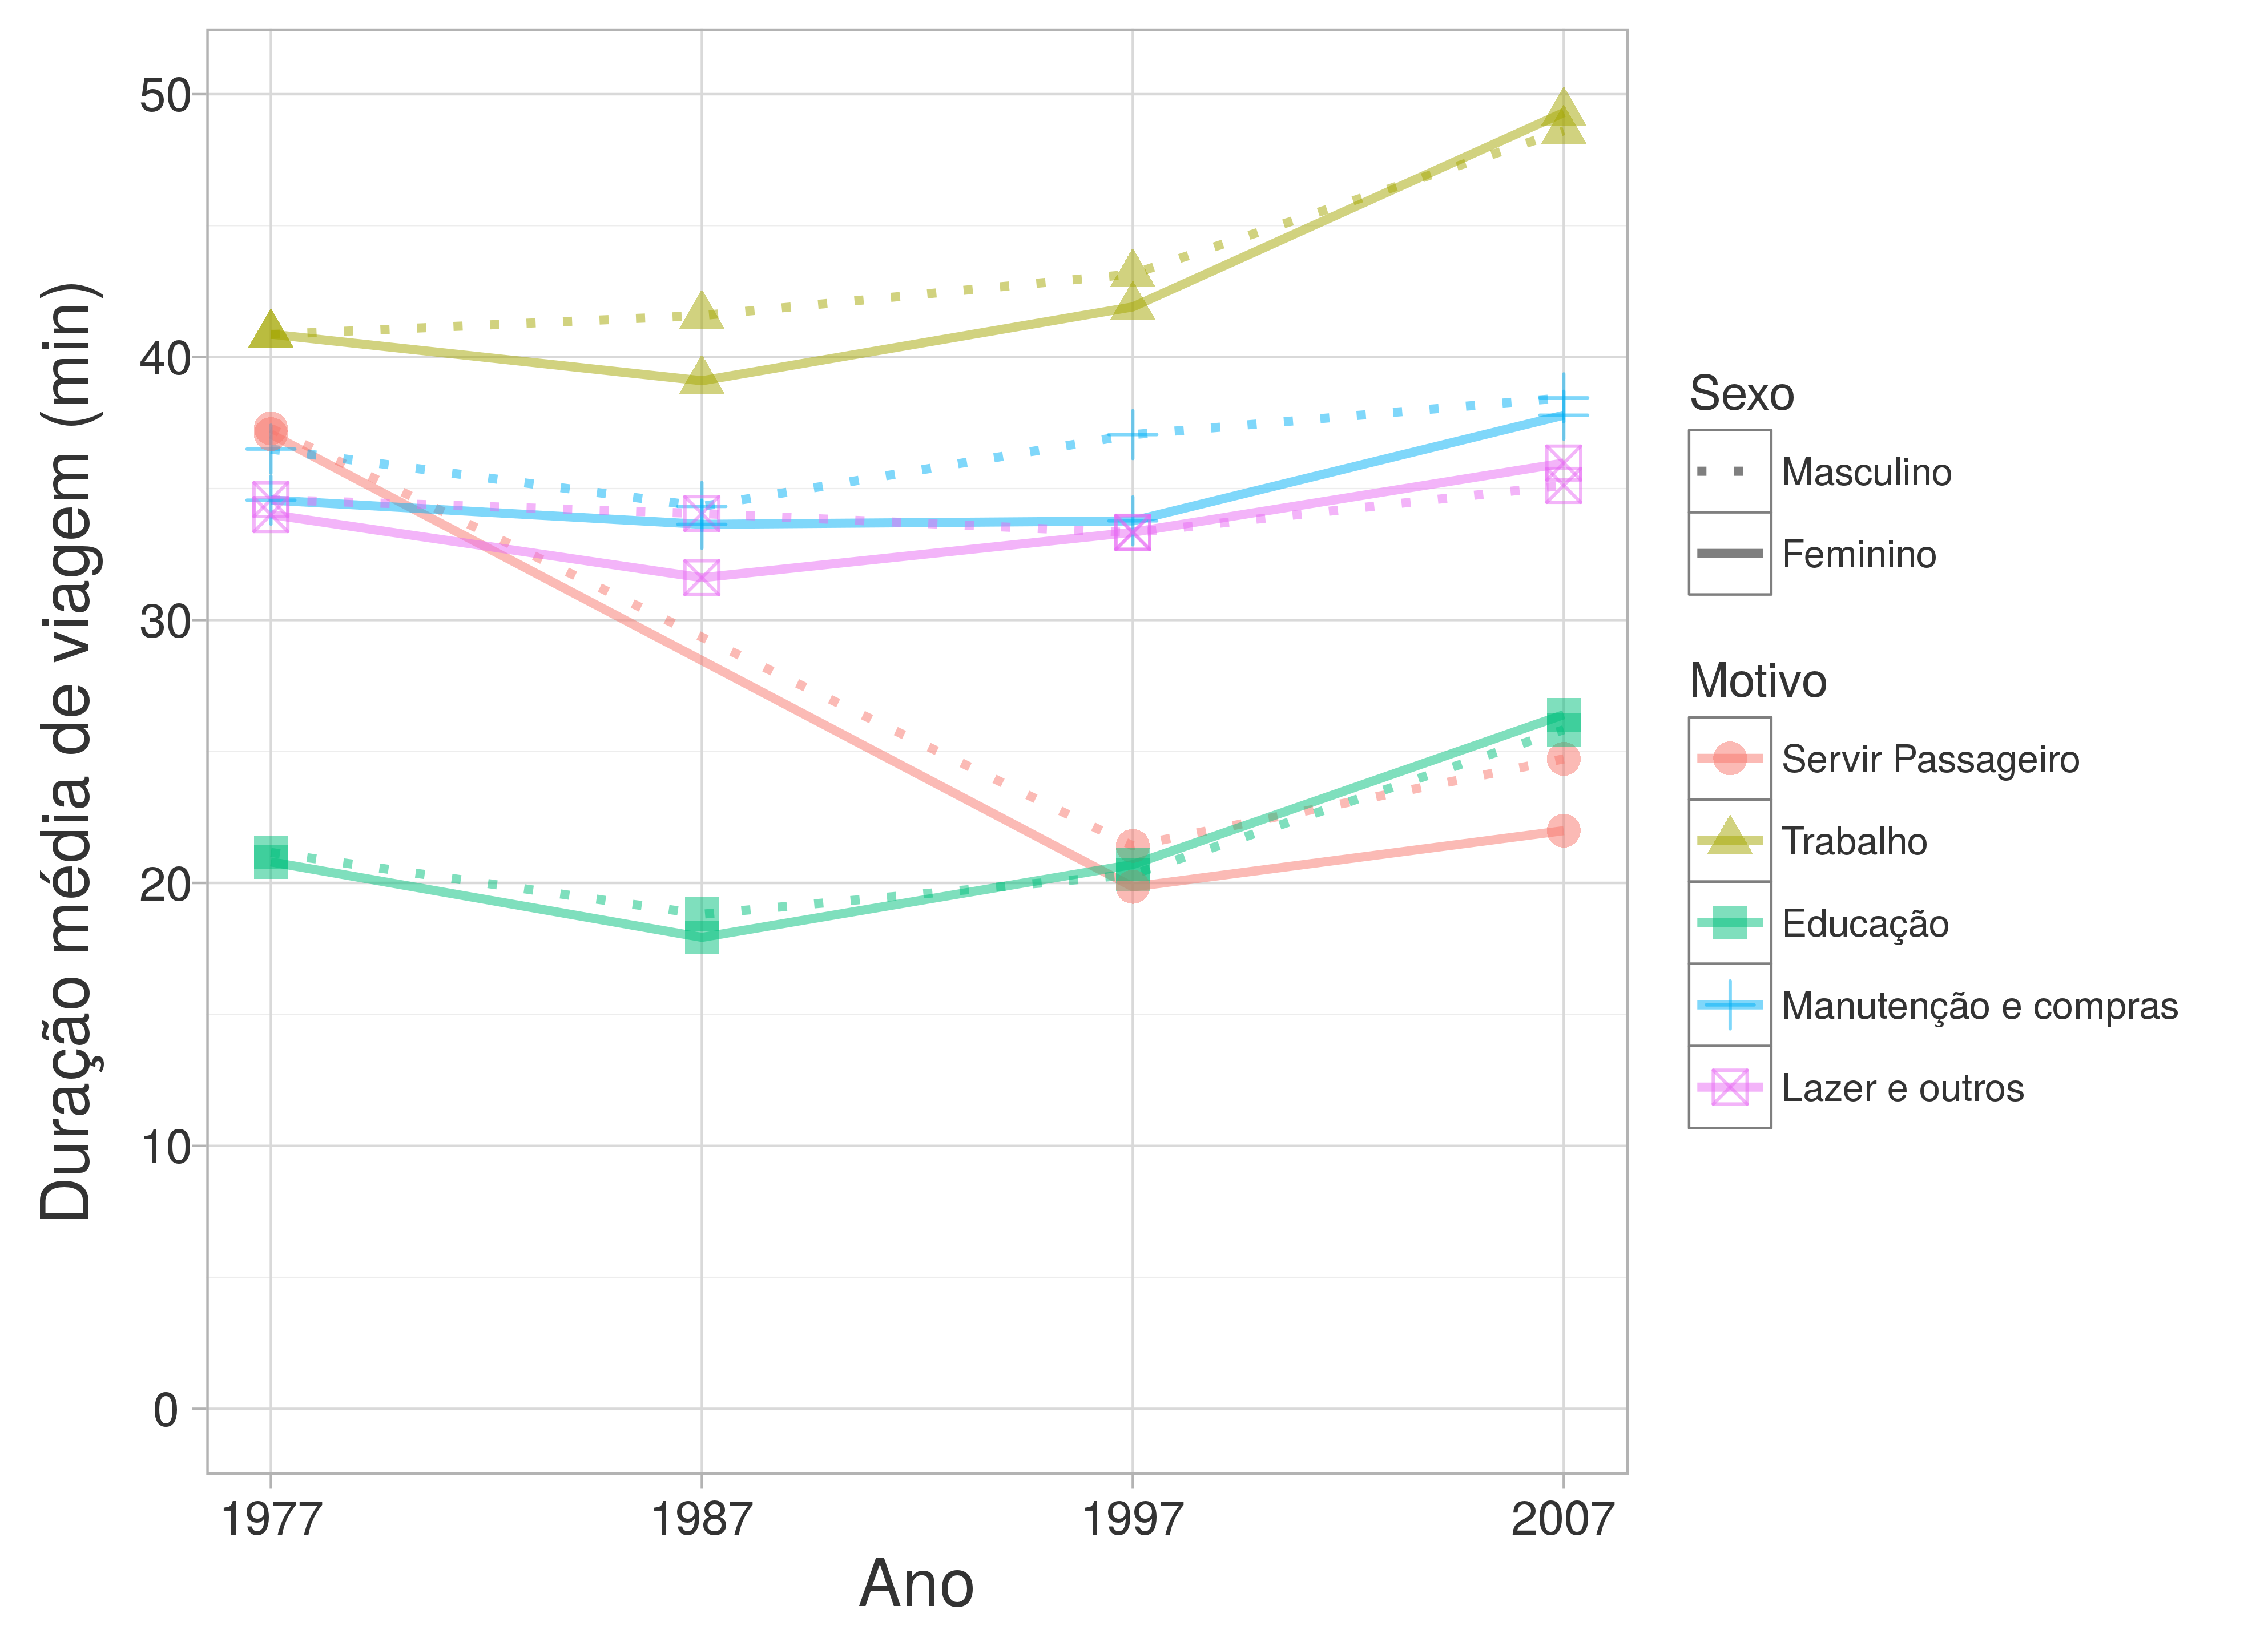
\includegraphics[width=1\textwidth]{./imagens/duracao-motivo.png}%
    \end{center}%
%    \fonte{Compilação própria}
\end{grafico}%
% Estatísticas para registros com F_VIAG==1 e SEXO
% Expandido com FE_VIAG

%TODO ?? Fazer DURACAO (médias) por faixas etárias / situação familliar
%Tendo em vista ainda as questões apontadas na revisão de literatura a respeito da mobilidade/imobilidade das pessoas e formas de mensurá-la, pretende-se avaliar a distância média das viagens em função das variáveis sexo, idade, renda familiar, renda individual, estado civil e presença de filhos da família \cite{ROSENBLOOM2006,SHEARMUR2006,HANSON2010}.

Em “Estatísticas sob Suspeita”, \citeauthoronline{CARRASCO2012} (\citeyear{CARRASCO2012}, p.100-101) propõe indicadores com base na experiência das mulheres e, especificamente, no capítulo relativo ao acesso à mobilidade e ao planejamento territorial, recomenda a formulação e consideração dos seguintes indicadores quando da formulação de políticas públicas:
motivos dos deslocamentos, meio utilizado nos deslocamentos e distâncias dos deslocamentos, entre outros.
Anteriormente foram apresentados os panoramas de motivos e modos, agora, serão exploradas as distâncias de deslocamento.

A variável de distância da viagem (\textbf{DIST_VIAG}) contém a distância euclidiana entre as coordenadas de origem e as coordenadas de destino, com as limitações que a determinação dessas coordenadas impõem, já que foram calculadas a partir dos centroides das subzonas ou zonas (na ausência das subzonas). Ou seja, para 1977, as distâncias representadas são apenas as inter-zonais, pois não haviam dados disponíveis nem de subzonas nem de coordenadas. Para 1987 e 1997, cujos mapas de subzonas foram disponibilizados, as distâncias representadas são a inter-subzonas. Ainda para 1997, diversas distâncias de viagens não foram possíveis de ser calculadas porque o \textit{shapefile} obtido junto ao Metrô-SP não continha todas subzonas indicadas no banco de dados da Pesquisa OD correspondente. E para 2007, mediante a disponibilidade de melhores recursos tecnológico, as distâncias apresentadas são mais precisas e obtidas diretamente das coordenadas. Assim, os valores, análises e eventuais resultados decorrentes das distâncias de viagem precisam ser olhados com parcimônia. As principais estatísticas desta variável, cuja unidade é quilômetros, são apresentadas na Tabela \ref{tab:estat-distancia}.

Não existem \textit{missing values} neste campo e, considerando apenas viagens com distância superior a zero, independentemente do sexo, os valores mínimos são: 0,37 km para 1977, 0,35 km para 1987, 0,23 km para 1997 e 0,01 para 2007.
As medianas da distância de viagem, também independente do sexo, crescem ao longo do período analisado, saindo de 5,62 km em 1977 para 5,79 km em 2007.
Os valores de assimetria são todos positivos, indicando maior concentração à esquerda e cauda longa à direita da distribuição.
Os valores de curtose evidenciam não se tratar de distribuição normal.
A distância média geral de viagem sempre aumenta no período analisado: 0,5 km de 1977 para 1987, 0,13 km de 1987 para 1997 e 0,44 km de 1997 para 2007.

Analisando esses dados segmentados por sexo, observa-se que as distâncias médias das viagens do homens cresce década a década e é sempre superior às das mulheres.
As distâncias médias das viagens das mulheres também cresce no período saindo de 6,64 km em 1977 e chegando a 7,80 km em 2007, valor inferior média masculina em 1977.
As diferenças entre os valores médios de mulheres e homens gira em torno de 1,5 km: 1,2 km para 1977, 1,6 km para 1987, 1,7 km para 1997 e 1,3 km para 2007.
Foram feitos teste t para avaliar se as médias entre os sexos, para o mesmo ano, e entre os anos, para o mesmo sexo, eram diferentes. Com um intervalo de confiança de 95\%, todos o p-valores obtidos indicavam ser possível rejeitar a hipótese nula de que a diferença entre as médias estadas eram iguais a zero.

\begin{table}[htb]
\centering
   \IBGEtab{%\renewcommand{\arraystretch}{1.5}%%\ABNTEXfontereduzida%
        \renewcommand{\arraystretch}{1.5}
        \caption{Estatísticas da variável ``DIST_VIAG'', por ano}
        \label{tab:estat-distancia}
    }{%

    \begin{tabular}{ccccccc}
        \toprule
        \textbf{Total} & \multicolumn{6}{c}{\textbf{}} \\ \hline
        \textbf{ANO}   & \textbf{Média} & \textbf{Desvio Padrão} & \textbf{Mediana} & \textbf{Máximo} & \textbf{Assimetria} & \textbf{Curtose} \\ \midrule \midrule
        \textbf{1977}  & 7,40 & 6,06 & 5,62 &  70,38 & 1,91 & 5,71 \\ \hline
        \textbf{1987}  & 7,90 & 6,92 & 5,67 & 107,33 & 1,90 & 5,31 \\ \hline
        \textbf{1997}  & 8,03 & 7,64 & 5,69 &  82,27 & 1,86 & 4,85 \\ \hline
        \textbf{2007}  & 8,47 & 8,15 & 5,79 &  84,10 & 1,73 & 4,05 \\ \bottomrule          

        \textbf{Sexo feminino} & \multicolumn{6}{c}{\textbf{}} \\ \hline
        \textbf{ANO}   & \textbf{Média} & \textbf{Desvio Padrão} & \textbf{Mediana} & \textbf{Máximo} & \textbf{Assimetria} & \textbf{Curtose} \\ \midrule \midrule
        \textbf{1977}  & 6,64 & 5,47 & 5,04 &  65,91 & 2,00 & 6,62 \\ \hline
        \textbf{1987}  & 6,92 & 6,26 & 4,82 & 107,33 & 2,09 & 6,75 \\ \hline
        \textbf{1997}  & 7,09 & 6,89 & 4,90 &  82,27 & 1,95 & 5,27 \\ \hline
        \textbf{2007}  & 7,80 & 7,73 & 5,16 &  82,67 & 1,80 & 4,42 \\ \bottomrule     

        \textbf{Sexo Masculino} & \multicolumn{6}{c}{\textbf{}} \\ \hline
        \textbf{ANO}   & \textbf{Média} & \textbf{Desvio Padrão} & \textbf{Mediana} & \textbf{Máximo} & \textbf{Assimetria} & \textbf{Curtose} \\ \midrule \midrule
        \textbf{1977}  & 7,89 & 6,37 & 6,08 & 70,38 & 1,83 & 5,15 \\ \hline
        \textbf{1987}  & 8,57 & 7,26 & 6,31 & 81,19 & 1,78 & 4,59 \\ \hline
        \textbf{1997}  & 8,82 & 8,13 & 6,36 & 81,05 & 1,76 & 4,34 \\ \hline
        \textbf{2007}  & 9,08 & 8,48 & 6,44 & 84,10 & 1,66 & 3,71 \\ \bottomrule             

    \end{tabular}
    }{%
%		\fonte{Elaboração própria}
	}
\end{table}
% Estatísticas para registros com F_FAM==1, filtro por ANO
% Expandido com FE_FAM

Com o intuito de melhor explorar as distâncias médias das viagens analisando modos e motivos, foram elaborados os Gráficos \ref{graf:distancia-modo}, \ref{graf:distancia-coletivo} e \ref{graf:distancia-motivo}.
O Gráfico \ref{graf:distancia-modo} apresenta as distâncias médias de viagem do transporte coletivo, individual e a pé, para homens e para mulheres. Verifica-se que:
\begin{compactitem}[]
\item (i) As distâncias médias de homens e mulheres são muito próximas para as viagens a pé ($\sim$ 75 m), sequer sendo estatisticamente significativa a diferença em 1997.
\item (ii) A distância média no transporte individual sobe em taxas crescentes a cada década (0,2 km de 1977 para 1987, 0,3 km de 1987 para 1997, e 0,5 km de 1997 para 2007).
\item (iii)  As diferenças nas distâncias médias de viagem feitas por transporte individual entre mulheres e homens aumenta de 1977 (1,7 km) para 1987 (1,9 km) e para 1997 (2,2 km), depois decresce em 2007 (2,1 km).
\item (iv) A distância média no transporte coletivo aumenta entre 1977 e 2007 para ambos sexos, sendo que o ritmo de crescimento vem diminuindo: diferença de 1,1 km entre 1977 e 1987, diferença de 0,5 km entre 1987 e 1997 e diferença de 0,4 km entre 1997 e 2007.
\item (v)  As diferenças nas distâncias médias de viagem feitas por transporte coletivo entre mulheres e homens aumenta de 1977 (1,3 km) para 1987 (1,7 km) e para 1997 (2,0 km), depois decresce em 2007 (1,4 km).
\end{compactitem}

\begin{grafico}[htb]%
    \caption{\label{graf:distancia-modo}Distâncias médias de viagem por ano e por sexo, segundo os modos (agregados)}%
    \begin{center}%
        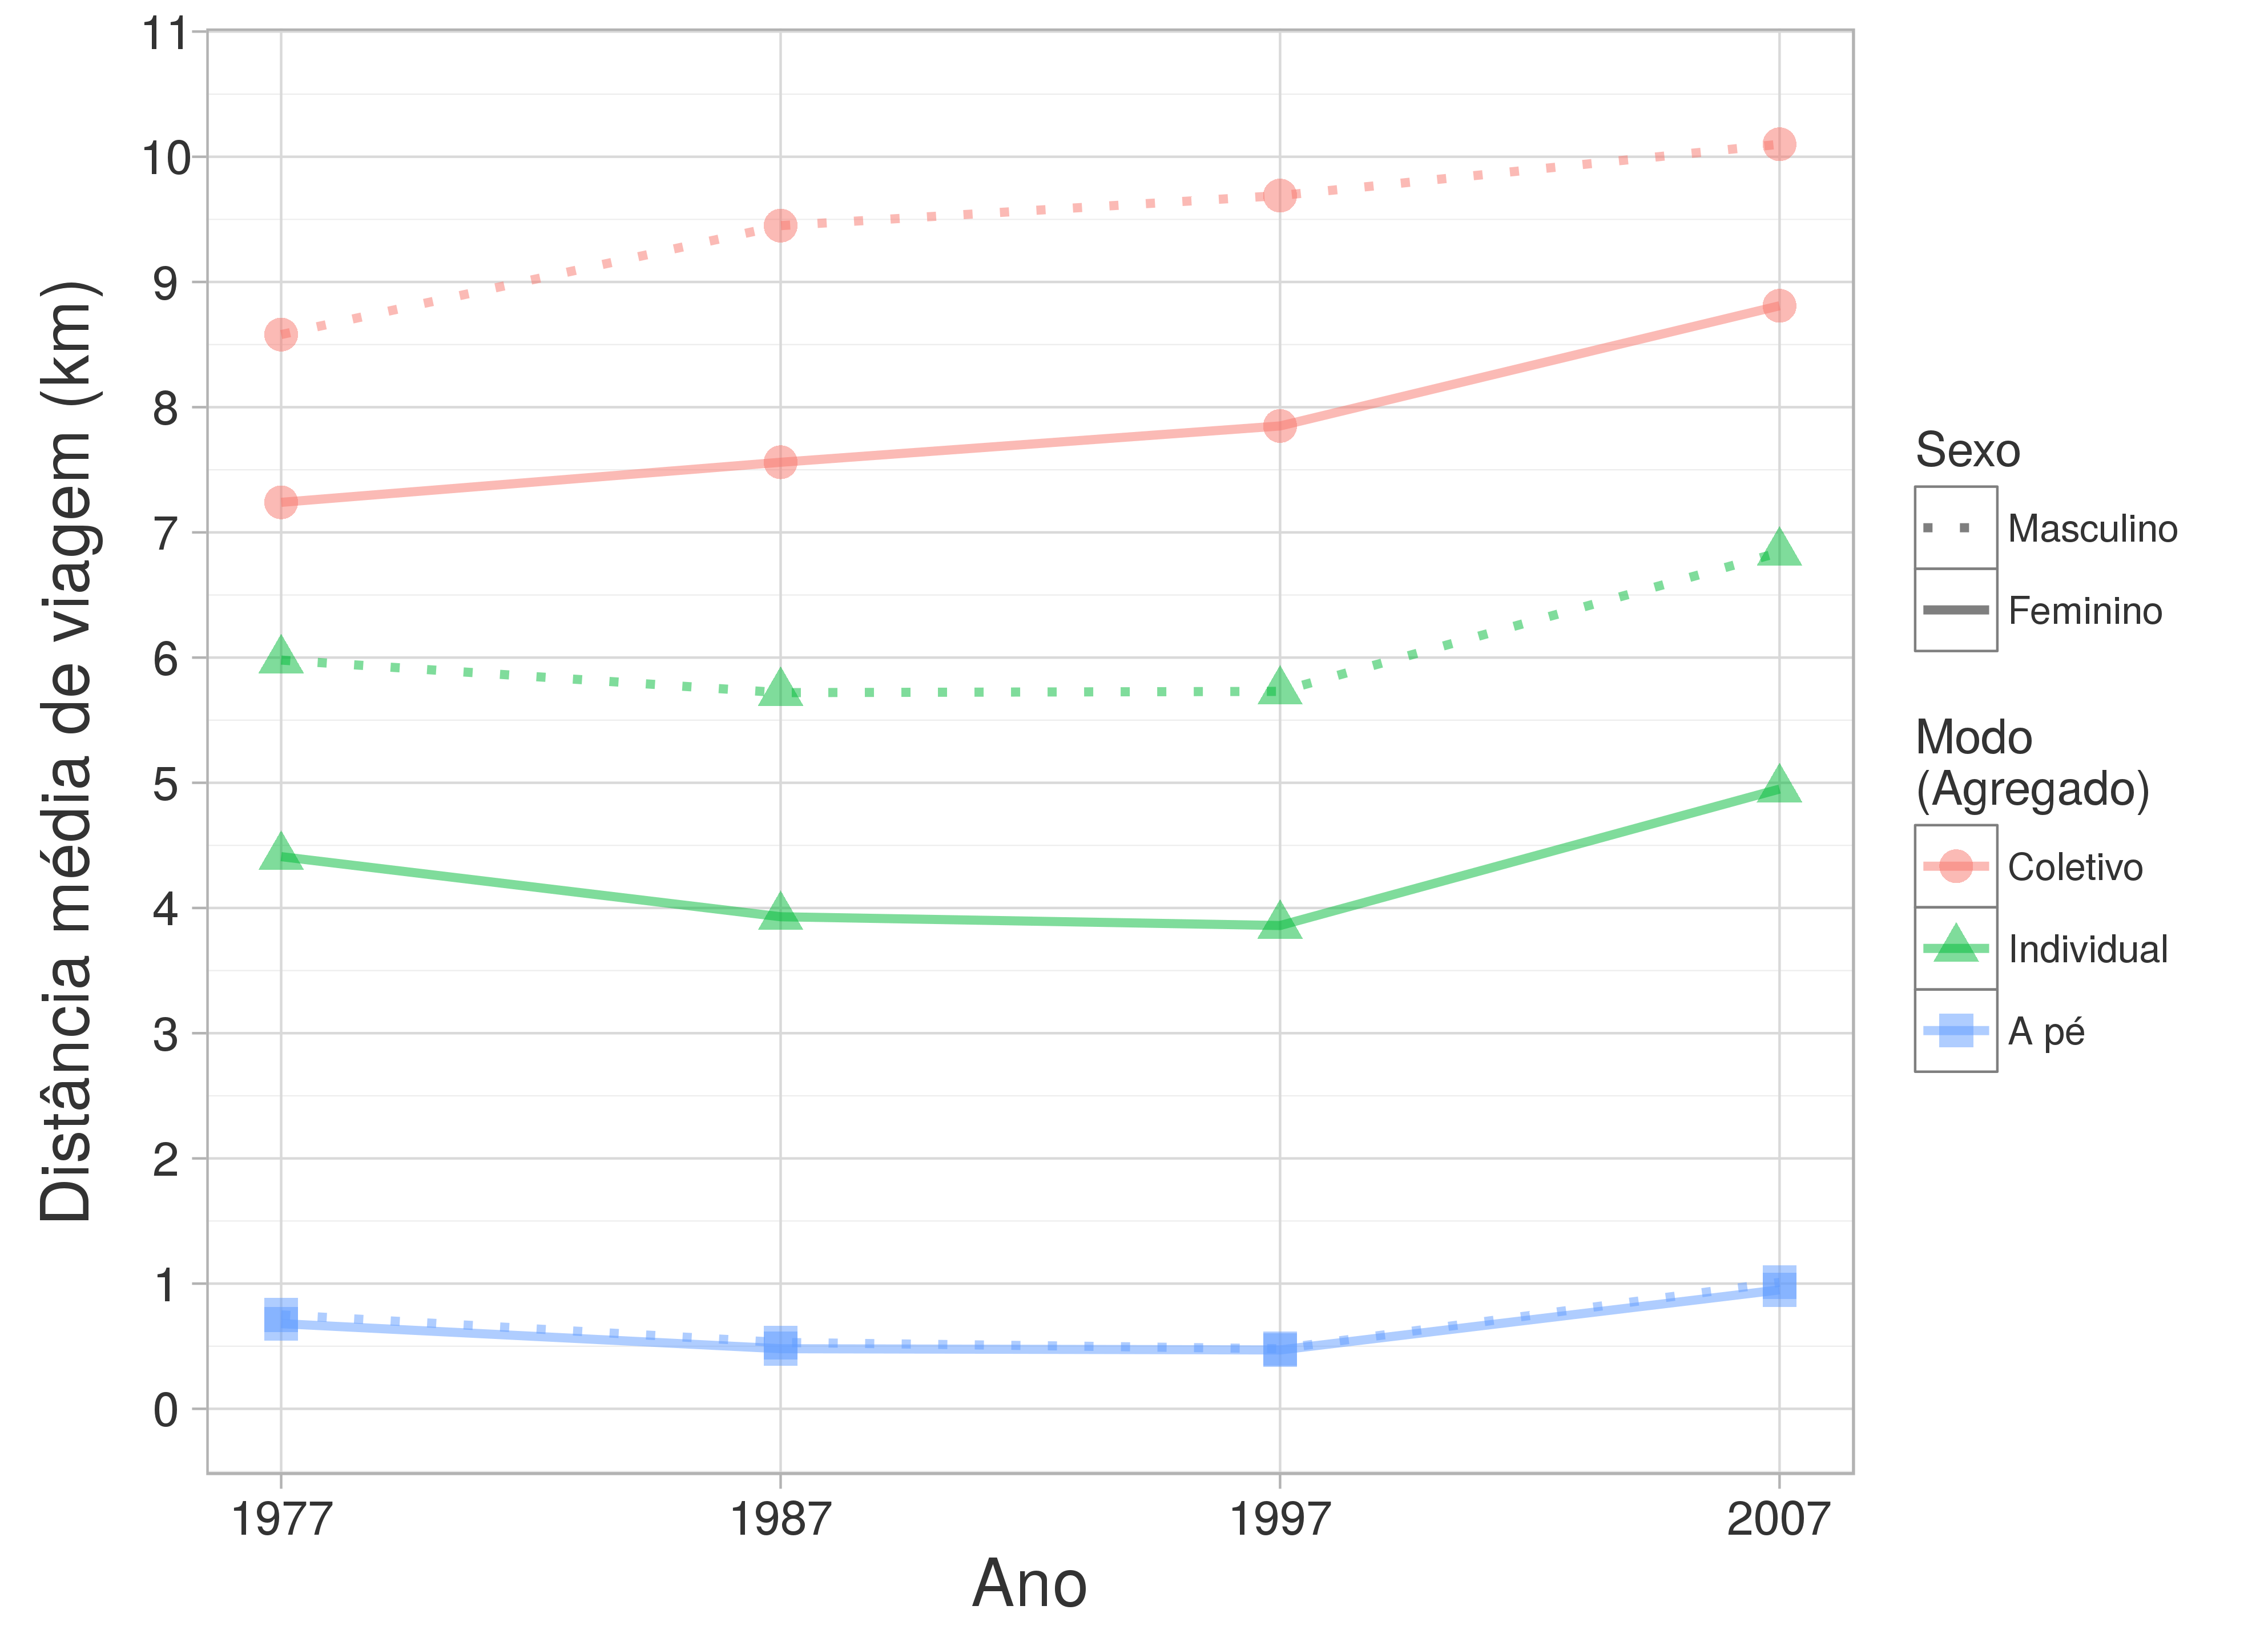
\includegraphics[width=1\textwidth]{./imagens/distancia-modo.png}%
    \end{center}%
%    \fonte{Compilação própria}
\end{grafico}%
% Estatísticas para registros com F_VIAG==1 e SEXO
% Expandido com FE_VIAG

\newpage

O Gráfico \ref{graf:distancia-coletivo} apresenta as distâncias médias dos modos de transporte coletivo (ônibus de linha, ônibus de empresa/escolar, lotação/perua/van/microônibus, Metrô e trem), para homens e para mulheres - foram separados os modos de alta capacidade dos demais para facilitar a compreensão dos gráficos. Verifica-se que:
\begin{compactitem}[]
\item (i) As distâncias médias de viagem de trem são superiores às de todos outros modos, inclusive o Metrô, com médias gerais caindo de 17,9 km em 1977 para 17,4 km em 1987, crescendo para 19,6 km em 1997 e tornando a cair em 2007 (19,4 km).
\item (ii) Para o trem, a distância média feminina só é superior à masculina em 1977 (diferença de 0,5 km), em 1987, 1997 e 2007 as médias delas são inferiores às deles (diferenças de 0,5 km, 1,8 km e 1,3 km, respectivamente).
\item (iii) As distâncias médias de viagem de Metrô crescem década a década, saindo 8,2 km em 1977, passando por 10,7 km em 1987, 12,0 km em 1977 e chegando a 13,4 km em 2007.
\item (iv) Para metrô, a distância média de viagem feminina é inferior à masculina, com diferenças de 0,3 km em 1977, 1,2 km em 1987, 1,5 km em 1997 e 0,5 km em 2007.
\item (v) As distâncias médias de viagem de ônibus de linha crescem sistematicamente, 0,8 km entre 1977 e 1987, 0,5 km entre 1987 e 1997, e 0,6 km entre 1997 e 2007.
\item (vi) Para ônibus de linha, as distâncias médias de viagem femininas são inferiores às masculinas, com diferenças de 1,1 km em 1977, 1,5 km em 1987, 1,7 km em 1997 e 1,3 km em 2007.
\item (vii) As distâncias médias de viagem de lotações/vans oscilam em torno de 10,9 km: sobem de 10,7 km em 1977 para 13,2 km em 1987, caem para 9,3 km em 1997 e tornando a aumentar em 2007 (10,5 km).
\item (viii) Para lotações/vans, as distâncias médias de viagem femininas são inferiores às masculinas exceto em 1987, com diferenças de 0,9 km em 1977, 4,1 km em 1987 (a mais para mulheres), 1,3 km em 1997 e 2,0 km em 2007.
\item (ix) As distâncias médias de viagem de ônibus escolar/fretado entre 1977 e 1987 não são estatisticamente diferentes. Há um crescimento nos valores de 1987 (8,8 km) para 1997 (9,1 km) e queda em 2007 (7,8 km).

\item (x) Para ônibus escolar/fretado, as distâncias médias de viagem femininas são inferiores às masculinas, com diferenças de 2,6 km em 1977, 2,3 km em 1987, 1,2 km em 1997 e 1,8 km em 2007.

\end{compactitem}

\begin{grafico}[htb]%
    \caption{\label{graf:distancia-coletivo}Distâncias médias de viagem por ano e por sexo, segundo os modos coletivos}%
    \begin{center}%
        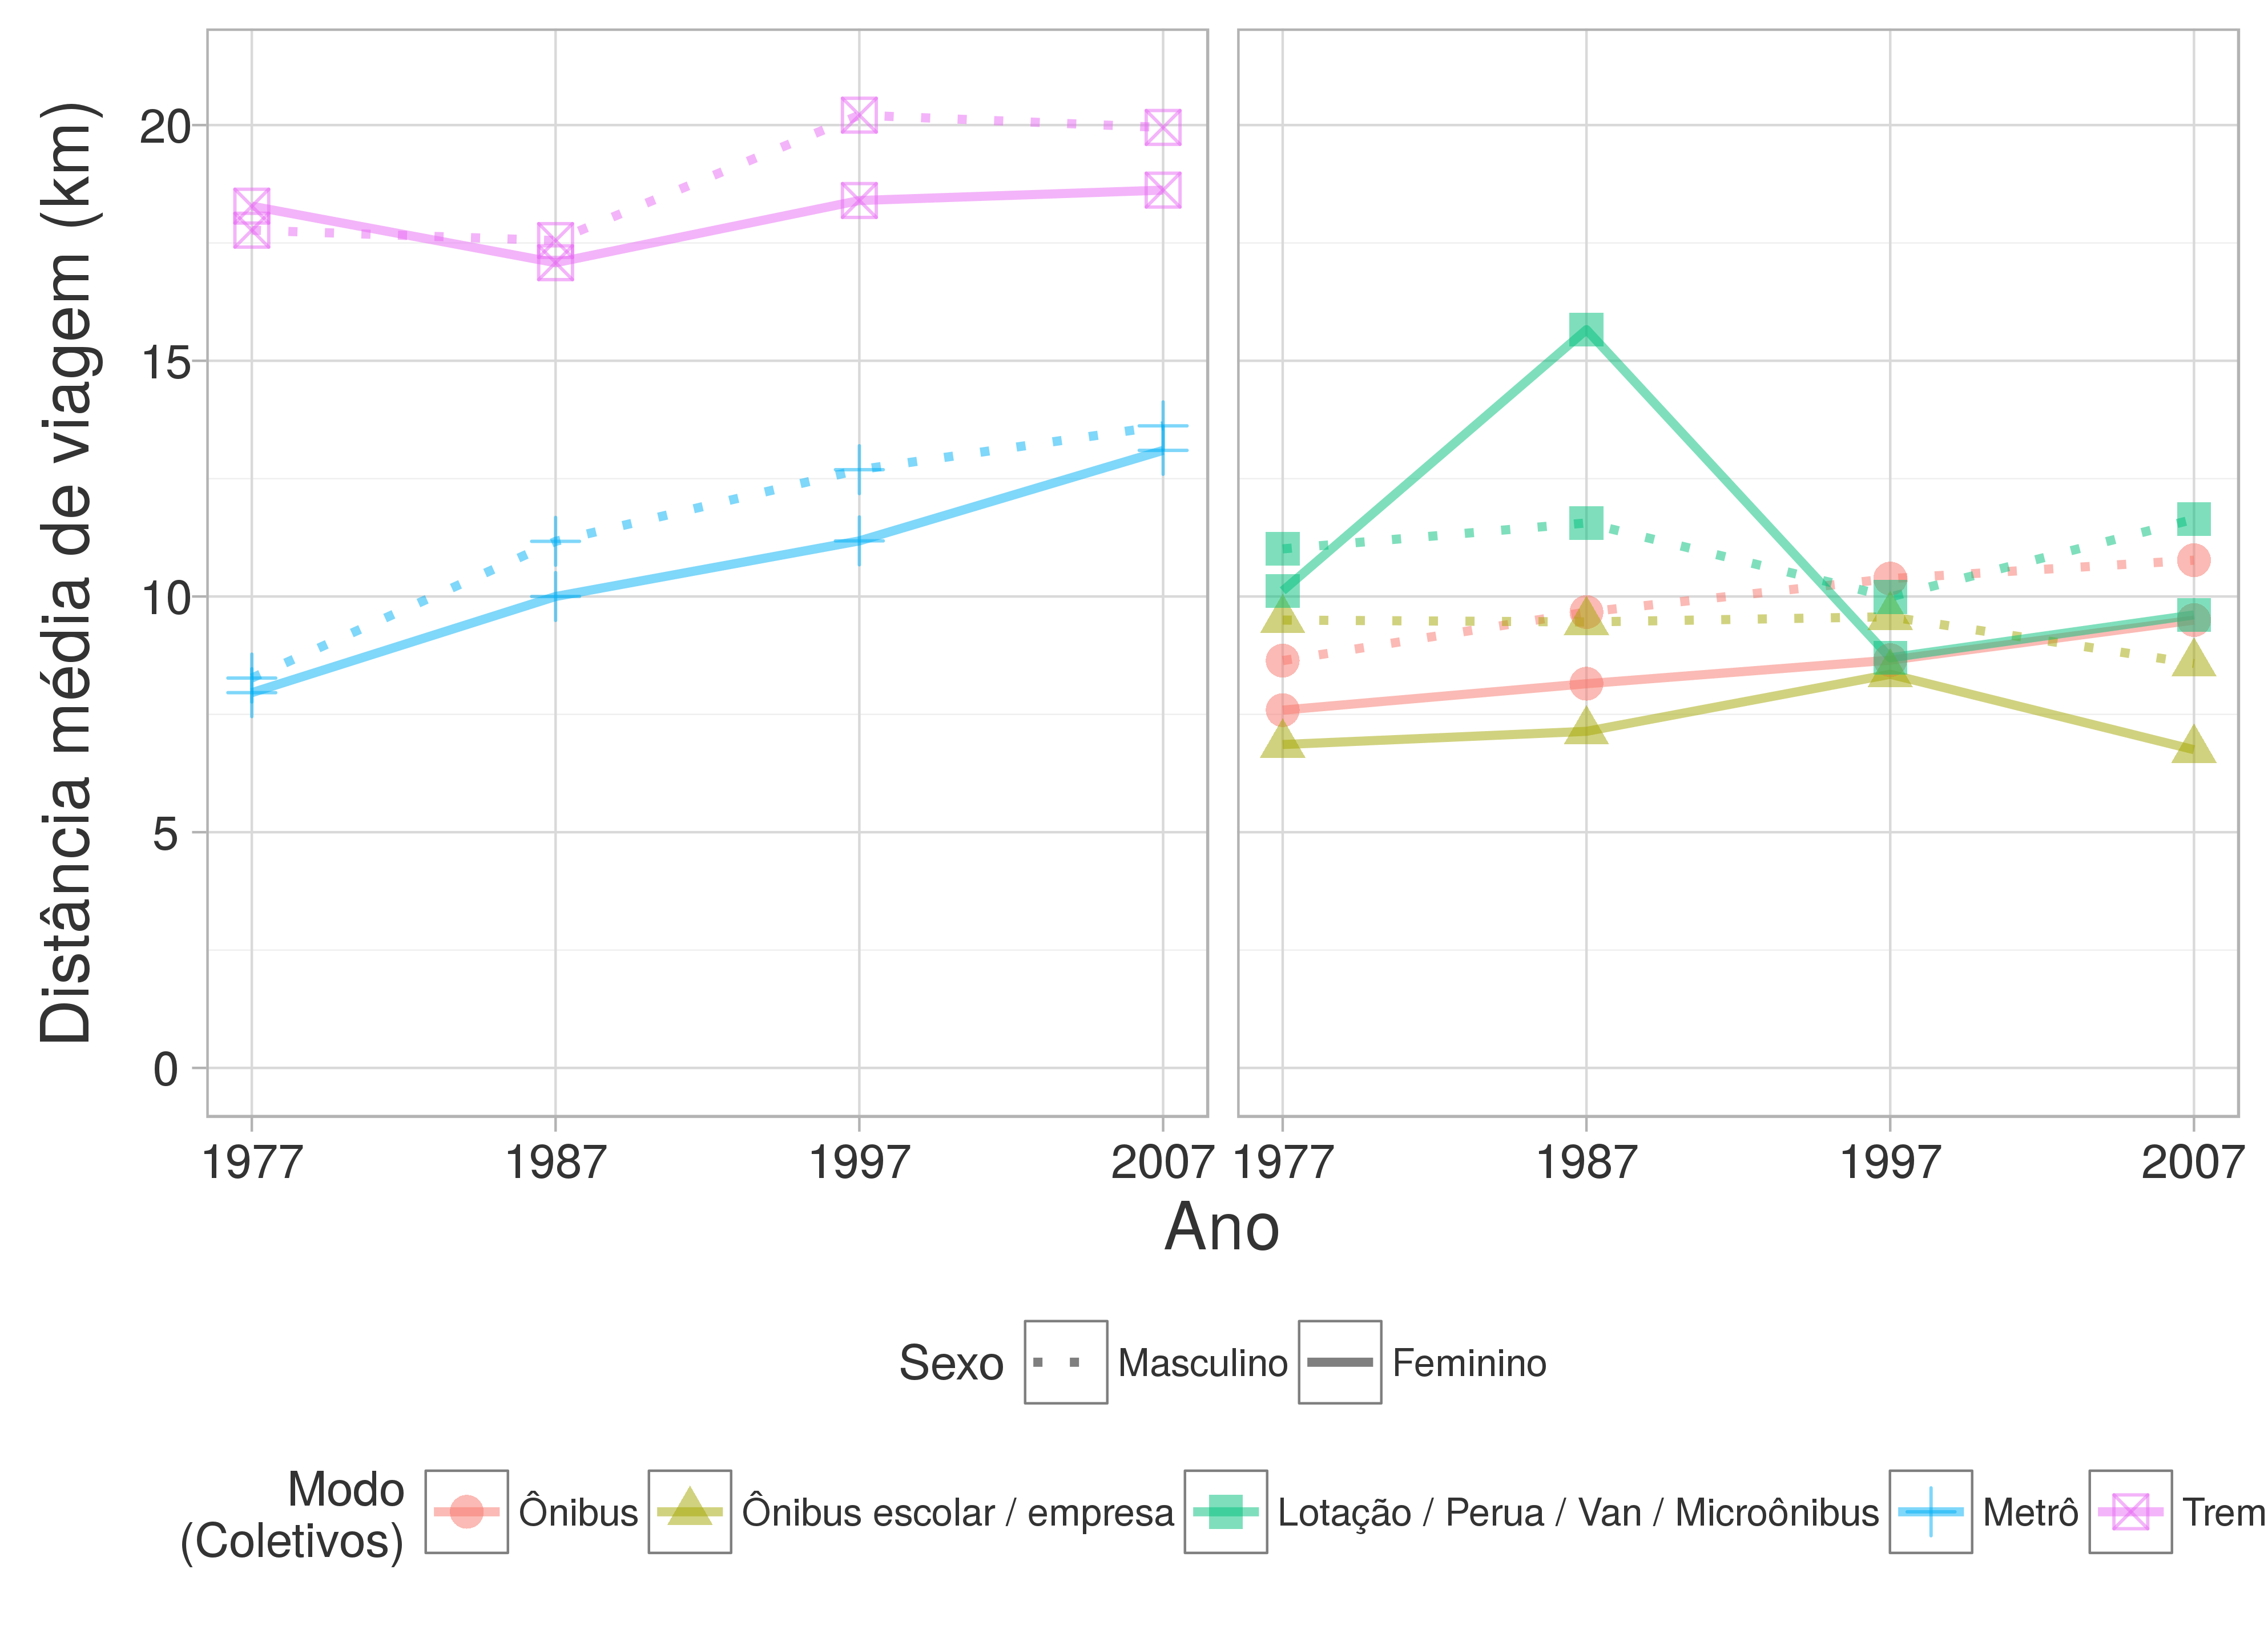
\includegraphics[width=1\textwidth]{./imagens/distancia-coletivo.png}%
    \end{center}%
%    \fonte{Compilação própria}
\end{grafico}%
% Estatísticas para registros com F_VIAG==1 e SEXO
% Expandido com FE_VIAG

\newpage

O Gráfico \ref{graf:distancia-motivo} apresenta as distâncias médias por motivo de viagem (trabalho, educação, servir passageiro, manutenção/compras e lazer/outros), para homens e para mulheres. Verifica-se que:
\begin{compactitem}[]
\item (i) As distâncias médias de viagem motivo trabalho (de natureza compulsória) são superiores a de todos outros motivos. Elas crescem ano a ano: 8,3 km em 1977, 9,2 km em 1987, 9,9 km em 1997 e 10,3 km em 2007.
\item (ii) Para viagens motivo trabalho (natureza compulsória), as distâncias médias femininas são sempre inferiores às masculinas, com diferenças girando em torno de 1,1 km: 0,8 km em 1977, 1,2 km em 1987, 1,3 km em 1977 e 1,0 km em 2007.
\item (iii) As distâncias médias de viagem motivo educação são as mais baixas frente ao demais motivos, exceto em 2007 quando servir passageiro assume média menor. Quando o motivos é escola, as distâncias meias caem de 1977 (5,44 km) para 1987 (5,23 km), e de 1987 para 1997 (5,16 km). Em 2007, os valores sobem novamente (5,87 km).
\item (iv) Para viagens motivo educação, as distâncias médias femininas são sempre inferiores às masculinas, com diferenças girando em torno de 0,4 km: 0,6 km em 1977, 0,7 km em 1987, 0,3 km em 1977 e, em 2007, a diferença não é estatisticamente significativa.
\item (v) As distâncias médias de viagem motivo manutenção/compras oscilam em torno de 6,9 km: passam de 6,6 km em 1977 para 7,1 km em 1987, caem para 6,9 km em 1997 e sobem novamente para 7,0 km em 2007. 
\item (vi) Para viagens motivo manutenção/compras, as distâncias médias femininas são sempre inferiores às masculinas, com diferenças girando em torno de 1,1 km: 1,1 km em 1977, 0,8 km em 1987, 1,7 km em 1977 e 0,8 km em 2007.
\item (vii) As distâncias médias de viagem motivo lazer/outros oscilam são crescentes no tempo: passam de 6,8 km em 1977 para 7,1 km em 1987, mantém o valor de 7,1 km em 1997 e sobem para 7,3 km em 2007. 
\item (viii) Para viagens motivo lazer/outros, as distâncias médias femininas são sempre inferiores às masculinas, com diferenças girando em torno de 0,9 km: 0,9 km em 1977, 1,2 km em 1987, 1,0 km em 1977 e 0,4 km em 2007.
\item (ix) As distâncias médias de viagem motivo servir passageiro decresce de 1977 (7,0 km) para 1997 (5,3 km), a partir de quando sobem até 2007 (5,8 km). Lembrando que em 1987 não havia o modo servir passageiro.
\item (x) Para viagens motivo servir passageiro, as distâncias médias femininas são sempre inferiores às masculinas, com diferenças crescentes: 0,1 km em 1977, 0,9 km em 1977 e 1,1 km em 2007.
\end{compactitem}


\begin{grafico}[htb]%
    \caption{\label{graf:distancia-motivo}Distâncias médias de viagem por ano e por sexo, segundo o motivo da viagem}%
    \begin{center}%
        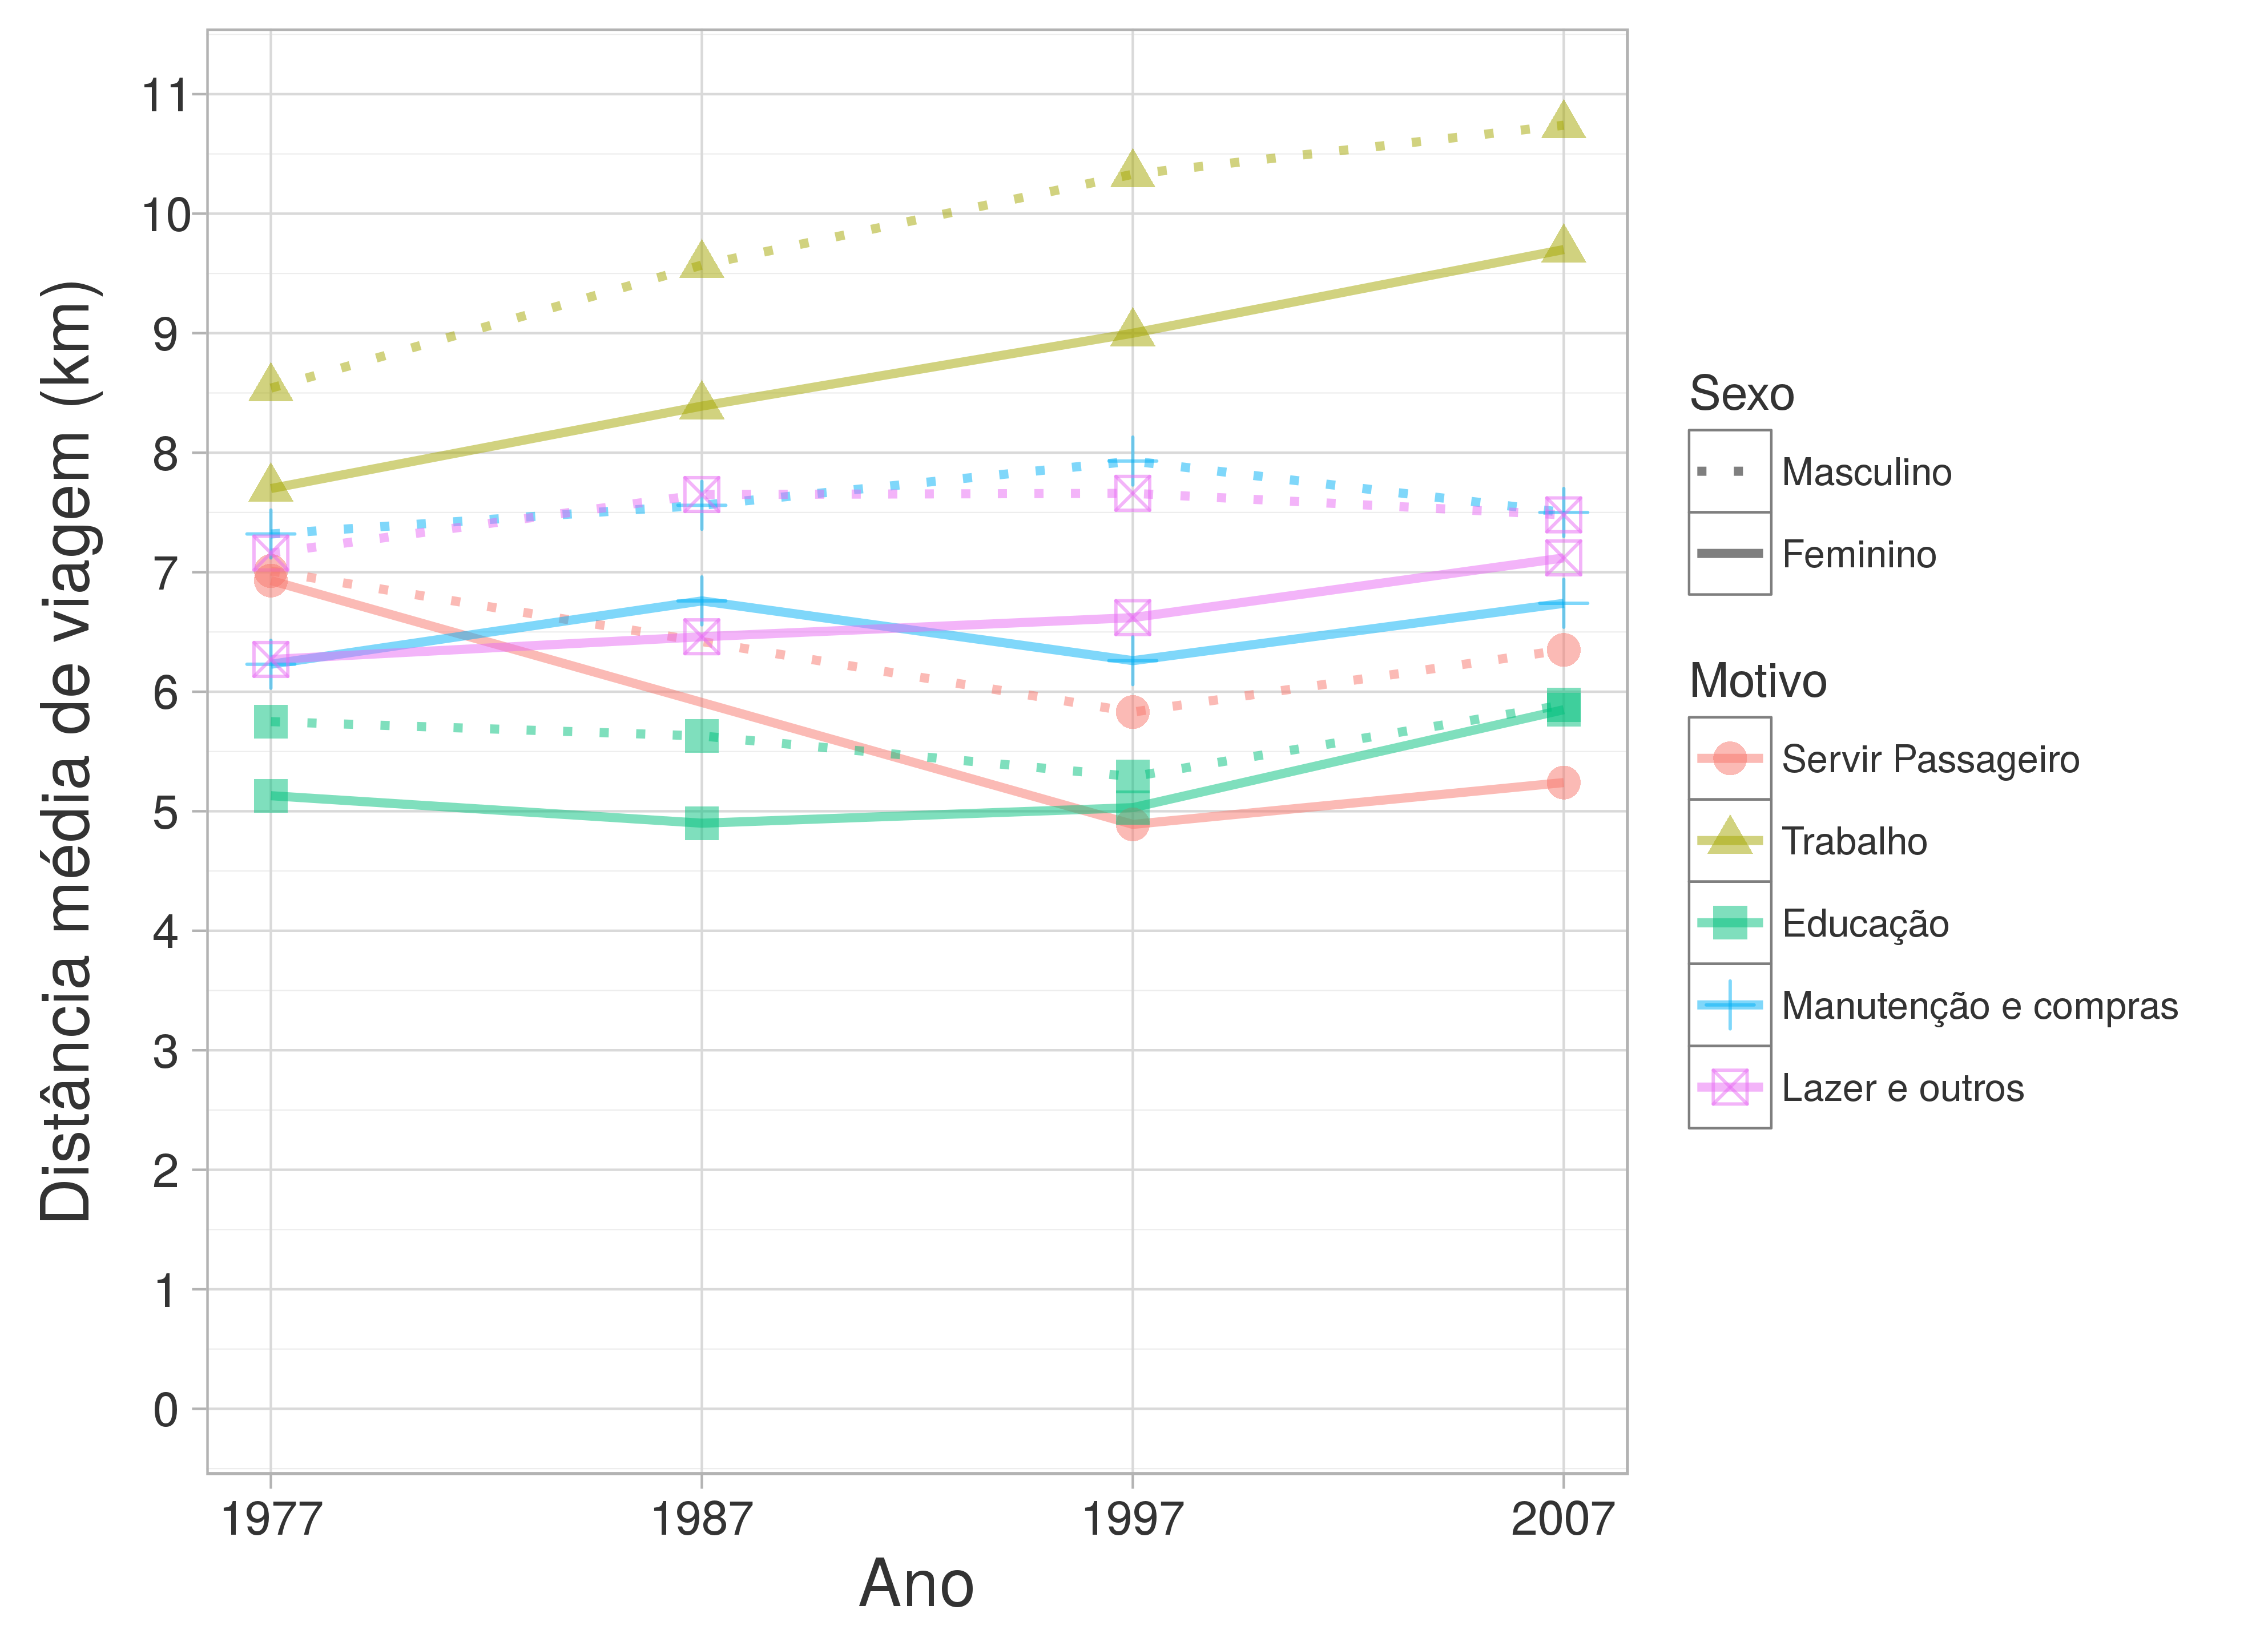
\includegraphics[width=1\textwidth]{./imagens/distancia-motivo.png}%
    \end{center}%
%    \fonte{Compilação própria}
\end{grafico}%
% Estatísticas para registros com F_VIAG==1 e SEXO
% Expandido com FE_VIAG









%TODO -> Fazer estatísticas de PESS_DIST_TOT
%Dalmaso e Strambi (2006) estudaram como o comportamento da distância total viajada por uma pessoa relaciona-se com seus atributos individuais sexo e idade.


\clearpage
\section{Análise de conglomerados para identificação de grupos}\label{sec:analises-clusters}

A análise de conglomerados tem como objetivo segregar elementos (observações) “em grupos homogêneos internamente, heterogêneos entre si e mutuamente exclusivos, a partir de determinados parâmetros conforme uma medida similaridade ou distância” \cite[p.196]{FAVERO2009}.  Esta técnica estatística de interdependência foi escolhida pois se deseja agrupar as pessoas, ou mesmo famílias, em grupos homogêneos em função da similaridade do comportamento de viagens.

%Vários trabalhos têm usados análises de agrupamento no estudo de XXXXX %TODO

Foi utilizada a função \textit{hclust} do pacote \textit{stats}
\footnote{Também existe a função \textit{agnes}, do pacote \textit{cluster}, cuja documentação está disponível em \url{https://cran.r-project.org/web/packages/cluster/cluster.pdf} e que se propõe a resolver o mesmo algoritmo. Porém, o resultado obtido dos três pacotes (stats, fastcluster e cluster) não foram iguais. \citeauthoronline{MURTAGH1975} (\citeyear{MURTAGH1975}) já apontavam divergência entre as funções \textit{hclust} e \textit{agnes} quando aplicadas à mesma matriz de distâncias.} \cite{RTEAM2011} para realizar as análises hierárquicas de conglomerados. Devido ao tamanho da base de dados e ao baixo desempenho em termos computacionais do pacote \textit{stats}, preferiu-se a função \textit{hclust} do pacote \textit{fastcluster}
\footnote{Detalhes da implementação disponível em \citeauthoronline{MULLNER2011} (\citeyear{MULLNER2011}).}. 
Segundo \citeauthoronline{MULLNER2013} (\citeyear{MULLNER2013}), no pior caso, a função do pacote \textit{stats} tem seu tempo de execução proporcional a $N^3$, já a mesma função no pacote \textit{fastcluster}, é poporcional a $N^2$. As análises de conglomerados não hierárquicas foram executadas pela função kmeans do pacote \textit{stats}. Na Figura \ref{fig:roteiro-cluster} pode-se observar os passos realizados nesta etapa de análise.

\begin{figure}[htb]%
    \caption{\label{fig:roteiro-cluster}Etapas para a realização de análise de conglomerados (\textit{clusters})}%
    \begin{center}%
        \includegraphics[width=0.30\textwidth]{./imagens/roteiro-cluster.eps}%
    \end{center}%
%    \fonte{Elaboração própria}
\end{figure}%


Na \textbf{etapa A}, foram delimitados dois conjuntos iniciais de variáveis de análise:
\begin{compactitem}
\item \textbf{conjunto I}: De atributos de viagem, relativas à família, a saber: FAM_DIST_TOT, FAM_DIST_MED, FAM_DURACAO_TOT, FAM_DURACAO_MED, FAM_VIAG_TOT;
\item \textbf{conjunto II}: De atributos de viagem, relativas à pessoa, a saber: PESS_DIST_TOT, PESS_DIST_MED, PESS_DURACAO_TOT, PESS_DURACAO_MED, PESS_MODO_ONIBUS, PESS_MODO_DIRIG, PESS_MODO_PASS, PESS_MODO_TREM, PESS_MODO_MOTO, PESS_MODO_BICI, PESS_MODO_APE, PESS_MODO_OUTROS, PESS_NO_MODOS, PESS_MOTIVO_TRAB, PESS_MOTIVO_EDUC, PESS_MOTIVO_RES, PESS_MOTIVO_SERV_PAS, PESS_MOTIVO_MANUT_COMPRAS, PESS_MOTIVO_LAZER_OUTROS, PESS_NO_MOTIVOS, PESS_PER_MADRUG, PESS_PER_COM_MAN, PESS_PER_MANHA, PESS_PER_MEIODIA, PESS_PER_TARDE, PESS_PER_COM_NOI, PESS_PER_NOITE, PESS_NO_PERIODOS, TOT_VIAG.
\end{compactitem}

Ocorre em diversos bancos de dados, inclusive neste, de se desejar analisar variáveis cujas unidades e ordens de grandezas não são as mesmas.
\citeauthoronline{FARIA2009} (\citeyear{FARIA2009}) indica que há duas razões para padronizar dados: (i) "evitar que as unidades escolhidas para mensurar as características afetem arbitrariamente a similaridade entre indivíduos", e (ii) fazer com "que as características contribuam igualmente na avaliação da similaridade entre indivíduos". Se houver alguma unidade de medição que tenha uma amplitude maior que as demais (como é o caso das distâncias totais da família em relação à distância média da pessoa), ela terá maior peso na análise de \textit{cluster}. Então, para mitigar o efeito dessas diferenças é indicado padronizar os dados antes de submetê-los à análise de conglomerados. Ao fazer isso, o pesquisador assume que a importância da variável decresce conforme a variabilidade aumenta \cite{EVERITT2011}. Há diversas formas de fazer essa padronização, as mais comuns são \textit{z-scores} e normalização \cite{FAVERO2009}. Há também possibilidades como dividir pela mediana dos desvios absolutos ou pelos intervalos de valores da variável \apud{GNANA1995}{EVERITT2011}, porém, a complexidade deste últimos métodos não se justificam frente ao conjunto de dados em discussão. Assim, na \textbf{etapa B} do presente trabalho, foi feita padronização das variáveis pelo método \textit{z-scores} conforme Equações \eqref{eq:z-score}, \eqref{eq:media} e \eqref{eq:desvio-padrao}.

\begin{equation}\label{eq:z-score}
Z(x)_{i} = \frac{x_{i} - \bar{x}}{\sigma(x)}
\end{equation}
sendo:
\begin{equation}\label{eq:media}
\bar{x} = \frac{1}{n} \sum_{i=1}^{n} x_{i}
\end{equation}

\begin{equation}\label{eq:desvio-padrao}
\sigma(x) = \sqrt{\frac{1}{(n-1)} \sum_{i=1}^{n}(x_{i}-\bar{x})^2 }
\end{equation}

\newpage
Um dos principais problemas das técnicas de aglomeração não hierárquica (K-means) é definir de início o número de \textit{clusters} desejado \cite{HARTIGAN1985, FAVERO2009, EVERITT2011}. Existem algumas técnicas para essa determinação:

\begin{compactitem}[]
\item (i) A \textbf{\textit{upper tail rule}} que considera os valores de fusão como uma série. Calcula-se a média, desvio padrão, estatística t como o desvio normalizado a partir da média. Em seguida, calcula-se o desvio padrão para cada valor de fusão (assumida distribuição normal), seleciona o primeiro ``significativo'' como sendo aquele cuja estatística t exceda o nível de 5\% de significância. Assim, a hipótese nula é que o valor fusão do k-ésimo termo advém da distribuição normal dos valores de fusão \cite{MOJENA1977}.
\item (ii) O \textbf{índice RMSSTD} (\textit{root mean square standard deviation}), ou raiz quadrada do desvio padrão médio (ver Equação \eqref{eq:RMSSTD}, calcula a homogeneidade dos agrupamentos \cite{SHARMA1996}, de maneira que quanto mais compactos os grupos, menor o valor desta estatística.
 
\begin{equation}\label{eq:RMSSTD} 
RMSSTD = \sqrt{\frac{\displaystyle\sum_{\substack{i=1\\
j=1}}^{\substack{nc\\
d}}\displaystyle\sum_{k=1}^{n_{j}}(x_{k}-\bar{x}_{j})^2}{\displaystyle\sum_{\substack{i=1\\
j=1}}^{\substack{nc\\
d}}(n_{ij}-1)}}
\end{equation}

\item (iii) O \textbf{índice $R^2$ ajustado} (ver Equação \eqref{eq:RS}), indica dissimilaridade entre agrupamentos \cite{SHARMA1996}, assim, quanto mais alto o valor de $R^2$ ajustado, mais dissimilaridade existe entre os grupos. O pesquisador pode estabelecer um valor desejado para $R^2$ e, a partir daí, determinar o número de \textit{clusters}.

\begin{equation}\label{eq:RS} 
R^2 = \frac{\left[\displaystyle\sum_{\substack{i=1\\
j=1}}^{\substack{nc\\
d}}\sum_{k=1}^{n_{j}}(x_{i}-\bar{x}_{j})^2\right]-\left[\displaystyle\sum_{\substack{i=1\\
j=1}}^{\substack{nc\\
d}}\displaystyle\sum_{k=1}^{n_{ij}}(x_{k}-\bar{x}_{j})^2\right]}{\displaystyle\sum_{j=1}^{d}\displaystyle\sum_{k=1}^{n_{j}}(x_{k} - \bar{x}_{j})^2 }
\end{equation}

\item (iv) O \textbf{\textit{best cut}} é um método que se baseia em um dendrograma (representação bidimensional em forma de árvore) que deve ser cortado quando as diferenças entre grupos forem visualmente mais significativas. Nesta representação, as linhas são ligadas segundo níveis de similaridade que agregará os indivíduos \cite{EVERITT2011}.
\end{compactitem}

Então, primeiro foi realizada a aglomeração hierárquica para definir as quantidades grupos.
No método hierárquico, se há n observações (linhas), parte-se de n grupos, ou seja, existe uma observações por grupo. A partir de medidas de similaridade, num processo iterativo, as observações vão sendo agrupadas até que se chegue a um único grupo no final. Segundo \cite{MAXWELL1977}, primeiro é feita a conversão da matriz \textit{n versus p} de dados em uma matriz \textit{n versus n} de medidas de similaridade ou dissimilaridade, tendo-se \textit{n} unidades amostrais e \textit{p} características.
Optou-se por primeiro utilizar o \textbf{\textit{best cut}} com os dendrogramas
\footnote{Os dendrogramas gerados admitiram escala não-monotônica.} 
e, em seguida, seriam avaliados os índices \textbf{RMSSTD} e \textbf{$R^2$ ajustado} de 90\%.

As medidas de (dis)similaridade podem ser de distância, correlação ou associação, esta última indicada para variáveis qualitativas. Como as variáveis selecionadas na \textbf{etapa A} são métricas ou \textit{dummies}, são indicadas medidas de distância ou correlação. 
Na Tabela \ref{tab:dist-cluster} é possível observar algumas das principais medidas de dissimilaridade comumente utilizadas.
Optou-se, na \textbf{etapa C}, pela medida de distância euclidiana, indicada pela literatura \apud{HAIR2005}{FAVERO2009}, 
a ser adotada em conjunto com os métodos de agrupamento Ward \cite{WARD1963} e centroide. O arcabouço teórico indica que tanto as distâncias euclidianas quanto as euclidianas quadráticas resultarão nos mesmos \textit{clusters} e, no caso da função \textit{hclust} utilizada, a distância padrão calculada é a euclidiana.



\begin{table}[htb]
    \IBGEtab{
	    \renewcommand{\arraystretch}{2.8}
        \caption{Medidas de dissimilaridade utilizadas em análise de \textit{cluster}}
		\label{tab:dist-cluster}
    }{%
	    \begin{tabular}{ll}
        \toprule
		    \headerTabCenterCell{Medida} &
	   	    \headerTabCenterCell{Fórmula}\\
		    \midrule \midrule
						Distância Euclidiana &
						\begin{math}
						    d_{ij}=\left[\displaystyle\sum_{k=1}^{p}w_{k}^2(x_{ik}-x_{jk})^2\right]^{}1/_2
						\end{math} \\
		    %\midrule
						Distância \textit{city block} &
						\begin{math}
                d_{ij}=\displaystyle\sum_{k=1}^{p}w_{k}|x_{ik}-x_{jk}|
						\end{math} \\
				%\midrule
				    Distância de Minkowski &
				    \begin{math}
				        d_{ij}=\left(\displaystyle\sum_{k=1}^{p}w_{k}^{r}|x_{ik}-x_{jk}|^{r}\right)^{{}1/_r} \quad (r\geq1)
				    \end{math} \\
				%\midrule
				    Distância de Canberra &
				    \begin{math}
				        d_{ij}= \begin{cases}
				                  0 & \quad \text{for } x_{ik}=x_{jk}=0 \\
				                  \displaystyle\sum_{k=1}^{p}w_{k}|x_{ik}-x_{jk}|/(|x_{ik}|+|x_{jk}|) & \quad \text{for } x_{ik} \neq 0 \text{ or } x_{jk} \neq 0\\
				                \end{cases}
				    \end{math} \\
			\bottomrule	
		\end{tabular}
    }{%
		\fonte{\cite{EVERITT2011}}
		}
\end{table}

Na \textbf{etapa D}, foi feita a aglomeração para o \textbf{conjunto I} de variáveis da família e para o \textbf{conjunto II} de variáveis da pessoa, utilizando tanto o método Ward quanto o centroide, utilizando filtros que captassem a ocorrência da família (F_FAM=1) ou da pessoa (F_PESS=1), respectivamente, para que não houvesse repetição indevida de famílias ou pessoas. Essas aglomerações foram feitas sem distinção dos anos e resultaram nos dendrogramas apresentados nas Figuras \ref{fig:cluster-fam-total} e \ref{fig:cluster-pess-total}. Percebe-se que a forma do dendrograma difere muito pouco entre os métodos Ward e centroide para o mesmo conjunto de variáveis.
%Para as análises seguintes foi escolhido o centroide pois segundo \apudonline{HAIR2005}{FAVERO2009}  “este método é mais robusto para observações atípicas”. 

Considerando o \textbf{best cut} observa-se que os dendrogramas que partiram das variáveis de família, indicam 4 como sendo um número de \textit{clusters} interessante de ser dado como \textit{input} do método K-means - observar seções S da Figura \ref{fig:cluster-fam-total}. Os índices \textbf{RMSSTD} e \textbf{$R^2$} ajustado, conforme pode ser visto no Gráfico \ref{graf:rmsstd-r2-cluster-fam-total}, também corroboram para a divisão em 4 grupos, representando 90\% da variância.

Partindo do conjunto de atributos de viagens relativas às pessoas, o \textbf{best cut} dos dendrogramas resultantes também indicam 4 \textit{clusters}, seja pelo método Ward, seja pelo centroide - observar seções S da Figura \ref{fig:cluster-pess-total}. Os índices \textbf{RMSSTD} e \textbf{$R^2$} ajustado, conforme pode ser visto no Gráfico \ref{graf:rmsstd-r2-cluster-pess-total}, também corroboram para a divisão em 4 grupos, representando mais de 90\% da variância.

Assim, na \textbf{etapa E}, definiu-se que seriam adotados 4 \textit{clusters}, tanto para o conjunto de variáveis I (de família) como o II (de pessoas) no método de aglomeração K-means
\footnote{ A função \textit{kmeans} do pacote \textit{stats} do software R implementa o algoritmo de \citeauthoronline{HARTIGAN1979} (\citeyear{HARTIGAN1979}) por padrão para sua execução, que utiliza também a distância euclidiana como medida de similaridade.} 
que, segundo \apudonline{GOUVEA2006}{FAVERO2009}, minimiza a variância interna aos grupos e maximiza a variância entre grupos.

\begin{figure}[htb]%
    \caption{\label{fig:cluster-fam-total}Dendrograma resultante da análise de conglomerados hierárquico, para o conjunto de atributos de viagens relativas às famílias}%
    \begin{center}%
        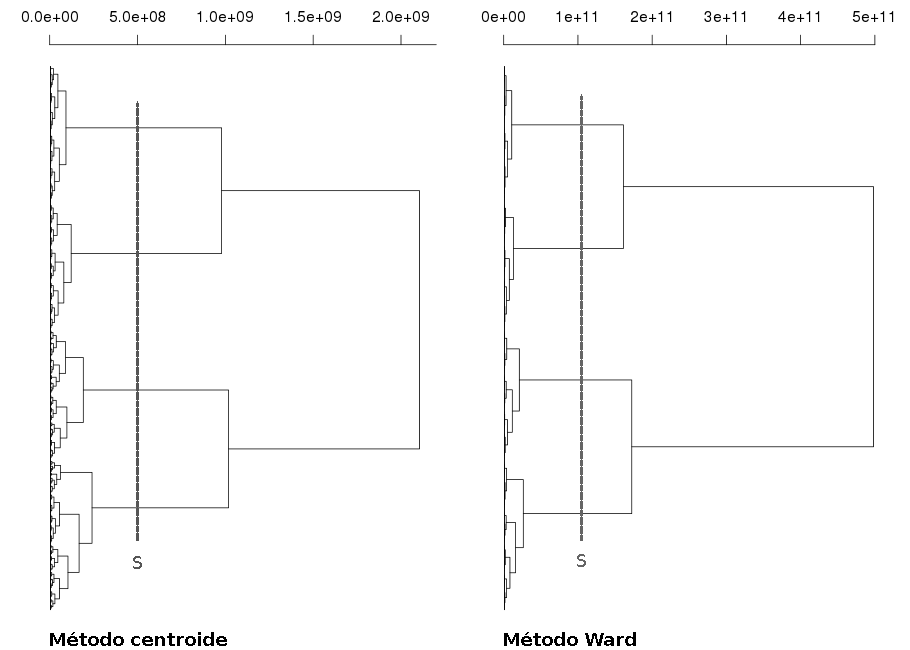
\includegraphics[width=0.95\textwidth]{./imagens/dendro-hierarq-cluster-familia-total-final.png}%
    \end{center}%
%    \fonte{Elaboração própria}
\end{figure}%


\begin{grafico}[htb]%
    \caption{\label{graf:rmsstd-r2-cluster-fam-total}Avaliação do número de \textit{clusters} para o conjunto de atributos de viagens relativas às famílias}%
    \begin{center}%
        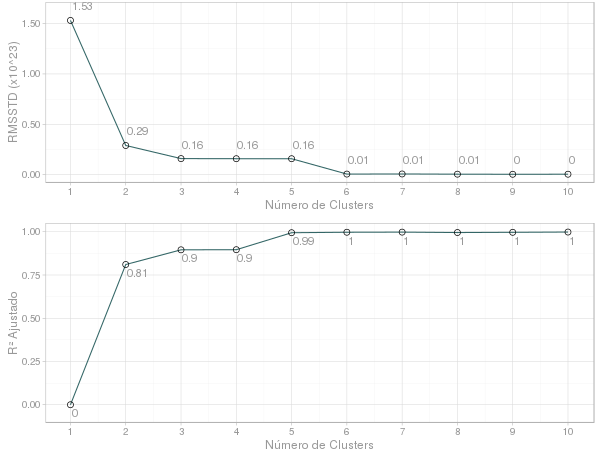
\includegraphics[width=0.8\textwidth]{./imagens/No-clusters-R2-RMSSTD-familia.png}%
    \end{center}%
%    \fonte{Elaboração própria}
\end{grafico}%


\begin{figure}[htb]%
    \caption{\label{fig:cluster-pess-total}Dendrograma resultante da análise de conglomerados hierárquico, para o conjunto de atributos de viagens relativas às pessoas}%
    \begin{center}%
        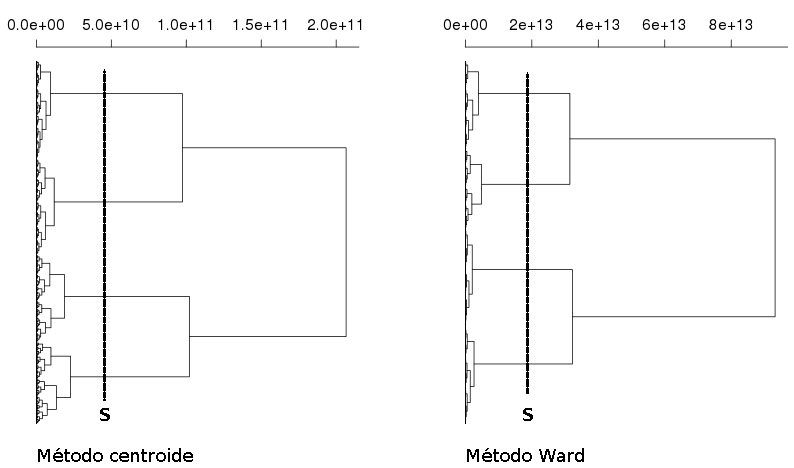
\includegraphics[width=0.95\textwidth]{./imagens/dendro-hierarq-cluster-pessoa-total-final.png}%
    \end{center}%
%    \fonte{Elaboração própria}
\end{figure}%

\clearpage

\begin{grafico}[htb]%
    \caption{\label{graf:rmsstd-r2-cluster-pess-total}Avaliação do número de \textit{clusters} para o conjunto de atributos de viagens relativas às pessoas}%
    \begin{center}%
        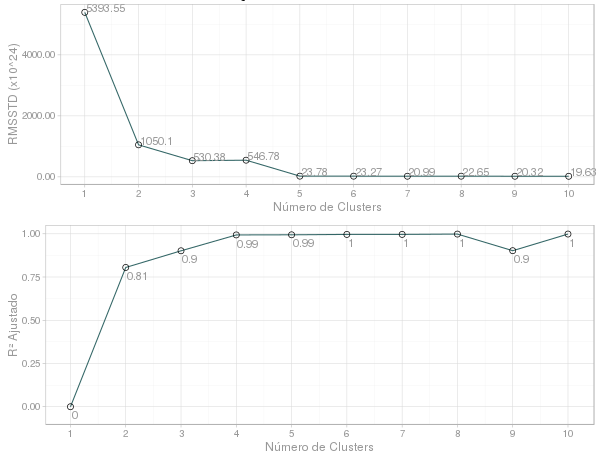
\includegraphics[width=0.8\textwidth]{./imagens/No-clusters-R2-RMSSTD-pessoas.png}%
    \end{center}%
%    \fonte{Elaboração própria}
\end{grafico}%

Na \textbf{etapa F}, foram formados então quatro agrupamentos para atributos de viagens de \textbf{família}, pelo método Ward. Observa-se que os grupos formados correspondem exatamente às observações de cada ano. 
Ou seja, o \textit{cluster} 1 agregou as observações de 1977, o \textit{cluster} 2 agregou as observações de 1987, e assim por diante - ver Tabela \ref{tab:cluster-fam-ward-4}. Entretanto, utilizando o método centroide, houve a união de 1997 e 2007, além da separação de 1987 em dois grupos distintos - ver Tabela \ref{tab:cluster-fam-centroide-4}.
Ao analisar os quatro agrupamentos para atributos de viagens de \textbf{pessoas}, tanto com o método centroide quanto com o Ward, os grupos formados também correspondem exatamente às observações de cada ano, como na Tabela \ref{tab:cluster-fam-ward-4}.

\begin{table}[htb]
    \IBGEtab{%\renewcommand{\arraystretch}{1.5}%%\ABNTEXfontereduzida%
%	    \renewcommand{\arraystretch}{1.5}
        \caption{Resultado do agrupamento de 4 \textit{clusters}, por atributos de viagens de família - método Ward}
		\label{tab:cluster-fam-ward-4}
    }{%
	    \begin{tabular}{P{1.00cm} P{3.00cm} P{3.00cm} P{3.00cm} P{3.00cm}}
            \toprule
	           \headerCenterCell{\textit{Cluster} nº} &
   	           \headerCenterCell{\% de famílias de 1977} &
   	           \headerCenterCell{\% de famílias de 1987} &   	           
   	           \headerCenterCell{\% de famílias de 1997} &   	           
   	           \headerCenterCell{\% de famílias de 2007}\\
		    \midrule \midrule
				1& % É  o 2, na verdade
		    	100&
		    	0&
		    	0&
				0\\
			\midrule
				2& % É o 1, na verdade
				0&
				100&
				0&
		        0\\
			\midrule
				3& % É o 3 mesmo
				0&
				0&
				100&
		        0\\
			\midrule
				4& % È o 4 mesmo
				0&
				0&
				0&
		        100\\
			\bottomrule	
		\end{tabular}
    }{%
		%\fonte{Elaboração própria}
	}
\end{table}

\begin{table}[htb]
    \IBGEtab{%\renewcommand{\arraystretch}{1.5}%%\ABNTEXfontereduzida%
%	    \renewcommand{\arraystretch}{1.5}
        \caption{Resultado do agrupamento de 4 \textit{clusters}, por atributos de viagens de família - método centroide}
		\label{tab:cluster-fam-centroide-4}
    }{%
	    \begin{tabular}{P{1.00cm} P{3.00cm} P{3.00cm} P{3.00cm} P{3.00cm}}
            \toprule
	           \headerCenterCell{\textit{Cluster} nº} &
   	           \headerCenterCell{\% de famílias de 1977} &
   	           \headerCenterCell{\% de famílias de 1987} &   	           
   	           \headerCenterCell{\% de famílias de 1997} &   	           
   	           \headerCenterCell{\% de famílias de 2007}\\
		    \midrule \midrule
				1& % É  o 3, na verdade
		    	100&
		    	0&
		    	0&
				0\\
			\midrule
				2& % É o 1, na verdade
				0&
				100&
				0&
		        0\\
			\midrule
				3& % É o 2, na verdade
				0&
				100&
				0&
		        0\\
			\midrule
				4& % È o 4 mesmo
				0&
				0&
				51,94&
		        48,06\\
			\bottomrule	
		\end{tabular}
    }{%
		%\fonte{Elaboração própria}
	}
\end{table}

\newpage
Tomando três agrupamentos, tendo em foco a \textbf{família}, pelo método Ward os grupos que se unem são os anos de 1997 e 2007. Já pelo método centroide, 1997 destaca-se de 2007, enquanto 1987 se agrega completamente a 1977, conforme pode ser observado nas Tabelas \ref{tab:cluster-fam-ward-3} e \ref{tab:cluster-fam-centroide-3}. Ao focar os atributos de viagens das \textbf{pessoas}, agrupadas em três \textit{clusters}, não houve diferença no resultado utilizando Ward ou centroide, tal como foi com quatro grupos,  conforme Tabela \ref{tab:cluster-pess-ward-centroide-3}.

\begin{table}[htb]
    \IBGEtab{%\renewcommand{\arraystretch}{1.5}%%\ABNTEXfontereduzida%
%	    \renewcommand{\arraystretch}{1.5}
        \caption{Resultado do agrupamento de 3 \textit{clusters}, por atributos de viagens de família - método Ward}
		\label{tab:cluster-fam-ward-3}
    }{%
	    \begin{tabular}{P{1.00cm} P{3.00cm} P{3.00cm} P{3.00cm} P{3.00cm}}
            \toprule
	           \headerCenterCell{\textit{Cluster} nº} &
   	           \headerCenterCell{\% de famílias de 1977} &
   	           \headerCenterCell{\% de famílias de 1987} &   	           
   	           \headerCenterCell{\% de famílias de 1997} &   	           
   	           \headerCenterCell{\% de famílias de 2007}\\
		    \midrule \midrule
				1& 
		    	100&
		    	0&
		    	0&
				0\\
			\midrule
				2& 
				0&
				100&
				0&
		        0\\
			\midrule
				3& % É o 3 mesmo
				0&
				0&
				46,5&
		        53,5\\
			\bottomrule	
		\end{tabular}
    }{%
		%\fonte{Elaboração própria}
	}
\end{table}

\begin{table}[htb]
    \IBGEtab{%\renewcommand{\arraystretch}{1.5}%%\ABNTEXfontereduzida%
%	    \renewcommand{\arraystretch}{1.5}
        \caption{Resultado do agrupamento de 3 \textit{clusters}, por atributos de viagens de família - método centroide}
		\label{tab:cluster-fam-centroide-3}
    }{%
	    \begin{tabular}{P{1.00cm} P{3.00cm} P{3.00cm} P{3.00cm} P{3.00cm}}
            \toprule
	           \headerCenterCell{\textit{Cluster} nº} &
   	           \headerCenterCell{\% de famílias de 1977} &
   	           \headerCenterCell{\% de famílias de 1987} &   	           
   	           \headerCenterCell{\% de famílias de 1997} &   	           
   	           \headerCenterCell{\% de famílias de 2007}\\
		    \midrule \midrule
				1&
		    	48,1&
		    	51,9&
		    	0&
				0\\
			\midrule
				2&
				0&
				0&
				100&
		        0\\
			\midrule
				3&
				0&
				0&
				0&
		        100\\
			\bottomrule	
		\end{tabular}
    }{%
		%\fonte{Elaboração própria}
	}
\end{table}


\newpage
Nota-se que 1977 e 1987 se separam, e 1997 se une a 2007. 
A variável ANO, embora não inserida nas análises de conglomerados, acabou sendo a grande diferenciadora dos grupos.
Esses resultados levantam a questões como:
\begin{compactitem}[]
\item (i) o tempo (em si ou como \textit{proxy} de outras variáveis) é uma categoria de análise relevante;
\item (ii) pode ter havido evolução no método de pesquisa e o agrupamento temporal esteja captando este efeito; 
\item (iii) deve haver semelhanças entre 2007 e 1997;
\item (iv) deve haver semelhanças entre 1987 e 1977, talvez mais fracas que aquelas entre 2007 e 1997;
\item (v) não parece haver semelhanças tão fortes entre 1987 e 1997. %TODO rever este item
\end{compactitem}
    
\begin{table}[htb]
    \IBGEtab{%\renewcommand{\arraystretch}{1.5}%%\ABNTEXfontereduzida%
	    \renewcommand{\arraystretch}{1.5}
        \caption{Resultado do agrupamento de 3 \textit{clusters}, por atributos de viagens de pessoas - métodos Ward e centroide}
		\label{tab:cluster-pess-ward-centroide-3}
    }{%
	    \begin{tabular}{P{1.00cm} P{3.00cm} P{3.00cm} P{3.00cm} P{3.00cm}}
            \toprule
	           \headerCenterCell{\textit{Cluster} nº} &
   	           \headerCenterCell{\% de pessoas de 1977} &
   	           \headerCenterCell{\% de pessoas de 1987} &   	           
   	           \headerCenterCell{\% de pessoas de 1997} &   	           
   	           \headerCenterCell{\% de pessoas de 2007}\\
		    \midrule \midrule
				1& 
		    	100&
		    	0&
		    	0&
				0\\
			\midrule
				2& 
				0&
				100&
				0&
		        0\\
			\midrule
				3&
				0&
				0&
				51,9&
		        48,1\\
			\bottomrule	
		\end{tabular}
    }{%
		%\fonte{Elaboração própria}
	}
\end{table}

Sob a perspectiva de gênero, retomando os dados de participação na PEA apresentados no Gráfico \ref{graf:evolucao-pea}, 
percebe-se o $\Delta_{1991-1980} = 6,3\%$, $\Delta_{2000-1991} = 11,2\%$ e $\Delta_{2010-2000} = 4,8\%$. Embora, os dados da PEA refiram-se aos anos 1980, 1991, 2000 e 2010, não coincidentes com os das Pesquisas OD (1977, 1987, 1997 e 2007), se tomarmos os anos mais próximos como referencial de análise, percebemos que o maior salto na participação feminina no mercado de trabalho ocorreu entre 2000 e 1991, e que as pesquisas que parecem apresentar a maior dissemelhança são as OD-1997 e OD-1987. Não é possível fazer muitas afirmações a partir somente deste paralelo, entretanto, isto pode ser um indicativo de que os padrões de mobilidade se alteraram sob efeito do tempo e também considerando o gênero como categoria de análise.
 
Para explorar melhor o que ocorre dentro de cada grupo e o que ocorre entre grupos foram analisadas as características de viagens, das pessoas e das famílias a partir da segregação dos 4 \textit{clusters} resultantes - ver Anexo \ref{chap:anexo_4_clusters_td}.

No agrupamento feito por atributos de viagens da \textbf{família} pelo método \textbf{Ward}, observa-se que a maior diferença percentual entre valores mínimo e máximo entre grupos ocorreu com a variável ``\% de pessoas com superior completo'' (76\%) e a menor diferença ocorreu com a variável ``sexo'' (4\%).
A Tabela \ref{tab:cluster-fam-ward-top10} apresenta as variáveis que apresentaram as diferenças percentuais entre valores máximos e mínimos superiores a 50\%.
Para estas nove variáveis foi realizado teste qui-quadrado de Pearson (de independência) em relação à variável ``nº de \textit{clusters}'' e todas mostraram-se significativas considerando um intervalo de confiança de 99\%. 

\begin{table}[htb]
    \IBGEtab{%\renewcommand{\arraystretch}{1.5}%%\ABNTEXfontereduzida%
	    \renewcommand{\arraystretch}{1.5}
        \caption{Ordenamento das variáveis pelas maiores diferenças percentuais - para agrupamento FAM_CLUSTER_WARD4}
		\label{tab:cluster-fam-ward-top10}
    }\\
		    \midrule \midrule
		    	1º&
				\% de pessoas com superior completo& 
				76\\
			\midrule
				2º& 
				\% de pessoas com situação famíliar `outros'&
		        71\\
			\midrule
				3º& 
				\% de famílias na Classe A&
		        67\\		        
			\midrule
				4º& 
				\% de pessoas com médio completo ou superior incompleto&
		        66\\	
			\midrule
				5º& 
				\% de pessoas que servem passageiro no destino&
		        65\\			        
			\midrule
				6º& 
				\% de famílias na Classe E&
		        61\\
			\midrule
				7º& 
				\% de famílias com presença de criança entre 0 e 4 anos&
		        60\\
			\midrule
				8º& 
				\% de pessoas empregadas&
		        59\\
			\midrule
				9º&
				\% de famílias com presença de criança entre 5 e 9 &
		        56\\
			\bottomrule	
		\end{tabular}
    }{%
		%\fonte{Elaboração própria}
	}
\end{table}

No agrupamento feito por atributos de viagens da \textbf{família} pelo método \textbf{centroide}, observa-se que a maior diferença percentual entre valores mínimo e máximo entre grupos ocorreu com a variável ``\% de famílias na Classe A'' (79\%) e a menor diferença ocorreu com a variável ``Média da quantidade de trabalhadores (as) na família'' (2\%).
Vale mencionar que as diferenças percentuais entre valores mínimo e máximo ocorreram entre os grupos 2 (uma parte de 1987) e 3 (outra parte de 1987) em relação as seguintes características: (i) distância média por viagem da pessoa; (ii) distância média por pessoa da família; (iii) \% de pessoas do sexo feminino e (iv) \% de outros parentes / agregados.

A Tabela \ref{tab:cluster-fam-centr-top10} apresenta as variáveis que apresentaram as diferenças percentuais entre valores máximos e mínimos superiores a 50\%.
Para estas nove variáveis foi realizado teste qui-quadrado de Pearson (de independência) em relação à variável ``nº de \textit{clusters}'' e todas mostraram-se significativas considerando um intervalo de confiança de 99\%. 

\begin{table}[htb]
    \IBGEtab{%\renewcommand{\arraystretch}{1.5}%%\ABNTEXfontereduzida%
	    \renewcommand{\arraystretch}{1.5}
        \caption{Ordenamento das variáveis pelas maiores diferenças percentuais - para agrupamento FAM_CLUSTER_CENTROIDE4}
		\label{tab:cluster-fam-centr-top10}
    }\\
		    \midrule \midrule
				1º& 
				\% de famílias na Classe A&
		        79\\		        
			\midrule
				2º& 
				\% de pessoas empregadas&
		        76\\
			\midrule			
		    	3º&
				\% de pessoas com superior completo& 
				73\\
			\midrule
				4º& 
				\% de pessoas com situação famíliar `outros'&
		        71\\
			\midrule
				5º& 
				\% de famílias na Classe E&
		        66\\
			\midrule
				6º& 
				\% de pessoas com médio completo ou superior incompleto&
		        65\\	
			\midrule
				7º& 
				\% de pessoas que servem passageiro no destino&
		        61\\			        
			\midrule
				8º& 
				\% de famílias na Classe E&
		        57\\
			\midrule
				9º& 
				\% de famílias com presença de criança entre 0 e 4 anos&
		        51\\
			\bottomrule	
		\end{tabular}
    }{%
		%\fonte{Elaboração própria}
	}
\end{table}

Oito dentre as nove variáveis listadas nas Tabelas  \ref{tab:cluster-fam-ward-top10} e \ref{tab:cluster-fam-centr-top10} repetem-se, indicando mais consistência do que divergência entre os métodos utilizados. Ao se dar importância para a ``\% de pessoas com superior completo'' ou ``\% de pessoas com médio completo ou superior incompleto'', na realidade, se está elencando a variável \textbf{grau de instrução} como relevante para explicar os agrupamentos. As porcentagens de famílias nas classes A, B ou E, colocam a \textbf{renda familiar} como outra variável relevante.
Raciocínio análogo se aplica entre a ``\% de pessoas com situação familiar outros'' e a \textbf{situação familiar} e entre a ``\% de pessoas que servem passageiro no destino'' e o \textbf{motivo no destino}.
\textit{Dummies} que indicam se a pessoa \textbf{trabalha ou não} ou \textbf{se há crianças até 9 anos} na família também são relevantes para explicar os agrupamentos.

Se tomado o mesmo procedimento com os \textit{clusters} resultantes dos atributos de viagem das pessoas (método centroide ou Ward), os resultados seriam idênticos aos obtidos no Anexo \ref{chap:anexo_4_clusters_td} (atributos de família, método Ward) e nas Tabelas \ref{tab:cluster-fam-ward-4} e \ref{tab:cluster-fam-ward-top10}, posto que o resultado dos agrupamentos foi o mesmo (por ano).

Seguindo recomendação de \citeauthoronline{VESPUCCI2003} (\citeyear{VESPUCCI2003}) foi feita uma análise de conglomerados a partir da primeira análise de conglomerados. Ou seja, o procedimento de análise de \textit{clusters} (hierárquico e não hierárquico) foi feito separadamente para 1977, 1987, 1997 e 2007, para os conjuntos de variáveis I (famílias) e II (indivíduos).
Analogamente ao Anexo \ref{chap:anexo_4_clusters_td} , o Anexo \ref{chap:anexo_4_clusters_fam} apresenta o resumo dos resultados quando formados os conglomerados a partir de atributos de viagens das famílias (método centroide) para cada ano.

Em 2007, foram formados os grupos CF01, CF02, CF03 e CF04, com 48.573, 41.870, 62.906 e 43.349 registros, respectivamente.
O grupo CF01 caracteriza-se por:
\begin{compactitem}
\item maior número médio de viagens por pessoa;
\item maiores durações (médias e totais) de viagens das pessoas e das famílias;
\item maior média da quantidade de trabalhadores(as) na família;
\item maior percentual de famílias com presença de trabalhadores(as).
\end{compactitem}

O grupo CF02 caracteriza-se por:
\begin{compactitem}
\item maiores distâncias (médias e totais) de viagens das pessoas e das famílias;

\item menor número de pessoas no conglomerado;
\item menor percentual de pessoas cuja situação familiar é ``empregado'';
\item maior percentual de pessoas com ensino médio completo ou superior incompleto;

\item menor número de famílias no conglomerado;
\item menor percentual de famílias com presença de 1 ou de 2 autos;
\item menor média da quantidade de automóveis na família;
\item maior percentual de famílias da classe C (com renda familiar entre 4 e 10 salários mínimos).
\end{compactitem}

O grupo CF03 caracteriza-se por:
\begin{compactitem}
\item maior número de registros no conglomerado;
\item maior número de viagens no conglomerado;
\item maior número médio de viagens (por pessoa e por família);
\item maior percentual de pessoas que servem passageiro no destino;
\item menores distâncias (médias e totais) de viagens das pessoas e das famílias;
\item menores durações (médias e totais) de viagens das pessoas e das famílias;

\item maior número de pessoas no conglomerado;
\item maior percentual de pessoas do sexo feminino;
\item maior média etária;
\item maior percentual de pessoas com superior completo;
\item maior percentual de pessoas que trabalham;
\item maiores percentuais de pessoas cuja situação familiar são ``pessoas responsável'', ``parentes/agregados'' e ``empregados(as)'';
\item menores percentuais de pessoas cuja situação familiar são ``cônjuge'' e ``filho(a)/enteado(a)'';
\item menor percentual de pessoas que estudam;

\item maior número de famílias no conglomerado;
\item maior percentual de famílias com presença de idosos com 60 anos ou mais;
\item maior percentual de famílias com presença de 1 ou mais;
\item maior média da quantidade de automóveis na família;
\item maior percentual de famílias das classes A e B (renda familiar maior a 10 salários mínimos);
\item maior média da renda (familiar e individual);
\item menor tamanho médio de família;
\item menores percentuais de famílias com presença de crianças (de 0 até 14 anos).
\end{compactitem}

O grupo CF04 caracteriza-se por:
\begin{compactitem}
\item menor número de viagens no conglomerado;
\item menor número médio de viagens (por pessoa e por família);
\item menor percentual de pessoas que servem passageiro no destino;

\item maior percentual de pessoas do sexo masculino;
\item maior percentual de pessoas que estudam;
\item maior percentual de pessoas de baixos graus de instrução (não alfabetizado, com ensino fundamental incompleto, com ensino fundamental completo ou ensino médio incompleto);
\item maiores percentuais de pessoas cuja situação familiar são ``cônjuge'' e ``filho(a)/enteado(a)'';
\item menores percentuais de pessoas cuja situação familiar são ``pessoas responsável'', ``parentes/agregados'', ``empregados(as)'' e ``outros'';
\item menor média etária;
\item menor percentual de pessoas que trabalham;

\item maior tamanho médio de família;
\item maiores percentuais de famílias com presença de crianças (de 0 até 14 anos);
\item maior percentual de famílias das classes D e E (renda familiar inferior a 4 salários mínimos);
\item menor média da renda (familiar e individual);
\item menor percentual de famílias com presença de idosos com 60 anos ou mais;
\item menor média da quantidade de trabalhadores(as) na família;
\item menor percentual de famílias com presença de 1 auto;
\item menor média da quantidade de automóveis na família.
\end{compactitem}

Destes resultados relativos a 2007 é possível conformar uma avaliação mais qualitativas dos grupos.
O CF01 o um grupo que mais concentra, percentualmente, os(as) trabalhadores(as). 
Majoritariamente são pessoas de famílias das classes C ou D, cujas viagens são as mais longas.

O CF02 é o grupo com o menor número de pessoas e de famílias do conglomerado e que concentra percentualmente as pessoas com grau de instrução intermediário (ensino médio ou superior incompleto), 
São pessoas de famílias menos motorizadas e com maior participação da classe C.
Quem está neste grupo realiza mais viagens mais distantes que as dos demais conglomerados, o que pode indicar que moram nas periferias e precisam deslocar-se mais todos os dias. 
Aqui, talvez esteja-se percebendo a ascensão das classes mais baixas engordando a classe C (aumento do nível de escolaridade e de renda, mas ainda residindo nas regiões periféricas).

O CF03 é um grupo mais feminino, mais velho e que concentra percentualmente as pessoas responsáveis pela família, possuindo as maiores rendas (individual e familiar) e o maior grau de instrução (superior completo). 
São pessoas de famílias menores, com menor percentual de crianças em sua composição, maior percentual de idosos e mais motorizadas.
Quem está neste grupo realiza mais viagens, que são mais curtas e mais rápidas que as dos demais conglomerados.
Como este grupo concentra as classes média alta e alta, provavelmente as pessoas/famílias têm residência localizadas em bairros mais bem servidos de infraestruturas e serviços, somado ao fato de disporem de carro (muitas vezes mais de um). Isso estimula a mobilidade, ou seja, possibilita fazer mais viagens (de menor distância a duração).

O CF04 é um grupo mais masculino, mais jovem e que concentra percentualmente os principais dependentes da família (cônjuges e filhos(as)). Este grupo apresenta os menores níveis de renda (individual e familiar) e também de escolaridade.
São pessoas de famílias maiores, com maior percentual de crianças em sua composição, menor percentual de idosos e baixas taxas de motorização.
Quem está neste grupo realiza menos viagens, o que pode indicar maior imobilidade.
Sendo o grupo com a menor média etária - a baixas idades correspondem baixos rendimentos - e o maior percentual de pessoas que estudam, este grupo concentra os(as) ``estudantes''.

Em 1997, foram formados os grupos CF05, CF06, CF07 e CF08, com 49.420, 47.294, 53.042 e 49.884 registros, respectivamente.
O grupo CF05 caracteriza-se por:
\begin{compactitem}
\item maior número médio de viagens por família;

\item menor número de pessoas no conglomerado;
\item maior percentual de pessoas cuja situação familiar é ``cônjuge'';

\item maior média da quantidade de trabalhadores(as) na família.
\end{compactitem}

O grupo CF06 caracteriza-se por:
\begin{compactitem}
\item menor número de registros no conglomerado;
\item menor número de viagens no conglomerado;
\item maiores distâncias totais de viagens das pessoas e das famílias;

\item maior percentual de pessoas que estudam;

\item menor número de famílias no conglomerado;
\item menor percentual de famílias com presença de idosos com 60 anos ou mais;
\item maior percentual de famílias com presença de trabalhadores(as);
\item maior percentual de famílias da classe C (com renda familiar entre 4 e 10 salários mínimos);
\item maior média da quantidade de trabalhadores(as) na família.
\end{compactitem}

O grupo CF07 caracteriza-se por:
\begin{compactitem}
\item maior número de registros no conglomerado;
\item maior número de viagens no conglomerado;
\item maior número médio de viagens por pessoa;
\item maior percentual de pessoas que servem passageiro no destino;
\item menores distâncias (médias e totais) de viagens das pessoas e das famílias;
\item menores durações (médias e totais) de viagens das pessoas e das famílias;

\item maior percentual de pessoas do sexo feminino;
\item maior média etária;
\item maior percentual de pessoas com , pelo menos, o ensino fundamental completo;
\item maior percentual de pessoas que trabalham;
\item maiores percentuais de pessoas cuja situação familiar são ``pessoas responsável'', ``parentes/agregados'', ``empregados(as)'' ou  ``outros'';
\item menores percentuais de pessoas cuja situação familiar são ``filho(a)/enteado(a)'';
\item menor percentual de pessoas que estudam;

\item maior número de famílias no conglomerado;
\item maior percentual de famílias com presença de idosos com 60 anos ou mais;
\item maior percentual de famílias com presença de 1 ou mais autos;
\item maior média da quantidade de automóveis na família;
\item maior percentual de famílias das classes A e B (renda familiar maior a 10 salários mínimos);
\item maior média da renda (familiar e individual);
\item menor tamanho médio de família;
\item menores percentuais de famílias com presença de crianças (de 0 até 14 anos).
\end{compactitem}

O grupo CF08 caracteriza-se por:
\begin{compactitem}
\item menor número médio de viagens (por pessoa e por família);
\item menor percentual de pessoas que servem passageiro no destino;
\item maiores distâncias médias de viagens das pessoas e das famílias;
\item maiores durações (médias e totais) de viagens das pessoas e das famílias;

\item maior número de pessoas no conglomerado;
\item maior percentual de pessoas do sexo masculino;
\item maior percentual de pessoas não alfabetizadas ou com ensino fundamental;
\item maiores percentuais de pessoas cuja situação familiar são ``filho(a)/enteado(a)'';
\item menores percentuais de pessoas cuja situação familiar são ``pessoas responsável'', ``cônjuge'', ``parentes/agregados'', ``empregados(as)'' e ``outros'';
\item menor média etária;
\item menor percentual de pessoas que trabalham;

\item maior tamanho médio de família;
\item maiores percentuais de famílias com presença de crianças (de 0 até 14 anos);
\item maior percentual de famílias das classes D e E (renda familiar inferior a 4 salários mínimos);
\item menor percentual de famílias com presença de idosos com 60 anos ou mais
\item menor percentual de famílias com presença de 1 ou mais autos;
\item menor média da quantidade de automóveis na família;
\item menor média da quantidade de trabalhadores(as) na família;
\item menor média da renda (familiar e individual).
\end{compactitem}

Dos resultados relativos a 1997 é possível conformar uma avaliação mais qualitativas dos grupos.
>>>> PAREI AQUI
O CF01 o um grupo que mais concentra, percentualmente, os(as) trabalhadores(as). 
Majoritariamente são pessoas de famílias das classes C ou D, cujas viagens são as mais longas.

O CF02 é o grupo com o menor número de pessoas e de famílias do conglomerado e que concentra percentualmente as pessoas com grau de instrução intermediário (ensino médio ou superior incompleto), 
São pessoas de famílias menos motorizadas e com maior participação da classe C.
Quem está neste grupo realiza mais viagens mais distantes que as dos demais conglomerados, o que pode indicar que moram nas periferias e precisam deslocar-se mais todos os dias. 
Aqui, talvez esteja-se percebendo a ascensão das classes mais baixas engordando a classe C (aumento do nível de escolaridade e de renda, mas ainda residindo nas regiões periféricas).

O CF03 é um grupo mais feminino, mais velho e que concentra percentualmente as pessoas responsáveis pela família, possuindo as maiores rendas (individual e familiar) e o maior grau de instrução (superior completo). 
São pessoas de famílias menores, com menor percentual de crianças em sua composição, maior percentual de idosos e mais motorizadas.
Quem está neste grupo realiza mais viagens, que são mais curtas e mais rápidas que as dos demais conglomerados.
Como este grupo concentra as classes média alta e alta, provavelmente as pessoas/famílias têm residência localizadas em bairros mais bem servidos de infraestruturas e serviços, somado ao fato de disporem de carro (muitas vezes mais de um). Isso estimula a mobilidade, ou seja, possibilita fazer mais viagens (de menor distância a duração).

O CF04 é um grupo mais masculino, mais jovem e que concentra percentualmente os principais dependentes da família (cônjuges e filhos(as)). Este grupo apresenta os menores níveis de renda (individual e familiar) e também de escolaridade.
São pessoas de famílias maiores, com maior percentual de crianças em sua composição, menor percentual de idosos e baixas taxas de motorização.
Quem está neste grupo realiza menos viagens, o que pode indicar maior imobilidade.
Sendo o grupo com a menor média etária - a baixas idades correspondem baixos rendimentos - e o maior percentual de pessoas que estudam, este grupo concentra os(as) ``estudantes''.


\clearpage
\section{Regressão logística para investigar a formação de grupos}\label{sec:analises-reg-log}

A regressão logística
\footnote{Técnica desenvolvida inicialmente por \citeauthoronline{COX1958} (\citeyear{COX1958}).}
%TODO Cox, DR (1958). "The regression analysis of binary sequences (with discussion)". J Roy Stat Soc B 20: 215–242.
 (binária) é uma técnica estatística que busca investigar a relação entre uma variável dependente categórica (neste caso uma \textit{dummy}) e variáveis explicativas métricas ou não métricas. Não se trata de um método de classificação, mas neste caso, é uma técnica que está sendo combinada após a utilização da análise de conglomerados, para tentar responder quais os pesos de cada variável na formação dos grupos (coincidente com os anos, na maior parte doas aglomerações).

As probabilidades são estimadas usando a função logística definida conforme Equações \eqref{eq:func-log} e \eqref{eq:Z}. Z (logit) assume valores entre menos e mais infinito, levando f(Z) a assumir valores entre 0 e 1, respectivamente. A ideia, analogamente à regressão linear, é construir uma função de predição que pondere as importâncias das variáveis explicativas na explicação de um determinado evento. Só é preciso ressaltar que na regressão linear, os estimadores correspondem às probabilidades, diretamente, já na regressão logística, o que se obtém, são scores do tipo $\operatorname(\mathbf{X}_i,k) = \boldsymbol\beta_k \cdot \mathbf{X}_i$,
onde \textit{Xi} é o vetor das variáveis descritivas por obervação i, \textit{k} é o vetor de pesos (ou coeficientes da regressão) correspondente à escolha \textit{k}.
Nos modelos de escolha discreta, as observações correspondem às pessoas que escolhem entre \textit{k} opções.
No presente caso, as observações correspondem às famílias ou às pessoas, que foram agrupadas num determinado \textit{cluster k}.
O termo \textit{(p/1-p)} é que representa, de fato, a chance de ocorrência do evento. 

\begin{equation}\label{eq:func-log}
f(Z) = \frac{1}{1+e^{-Z}}
\end{equation}
sendo:
\begin{equation}\label{eq:Z}
Z = \ln \left( \frac{p}{1 - p} \right) = \alpha + \sum\beta_{k}.X_{i} 
\end{equation}

Na regressão logística multinomial a variável dependente é categórica com duas ou mais categorias, de natureza ordinal ou nominal. Tomemos por linha de análise o caso intrigante em que os \textit{clusters} coincidem com os anos. Assim, tomando 2007 (categoria 4) por referência temos as Expressões \eqref{eq:Z1}, \eqref{eq:Z2} e \eqref{eq:Z3}.

\begin{equation}\label{eq:Z1}
Z = \ln \left( \frac{P(cluster=1|X)}{P(cluster=4|X)} \right) = \alpha_{1} + \sum\beta_{1}.X_{i} 
\end{equation}

\begin{equation}\label{eq:Z2}
Z = \ln \left( \frac{P(cluster=2|X)}{P(cluster=4|X)} \right) = \alpha_{2} + \sum\beta_{2}.X_{i} 
\end{equation}

\begin{equation}\label{eq:Z3}
Z = \ln \left( \frac{P(cluster=3|X)}{P(cluster=4|X)} \right) = \alpha_{3} + \sum\beta_{3}.X_{i} 
\end{equation}

Foram utilizadas tanto a função \textit{mlogit} da versão 11 do software estatístico STATA quanto a função \textit{multinom} do pacote \textit{nnet}
\footnote{Documentação do pacote \textit{nnet} disponível em \url{https://cran.r-project.org/web/packages/nnet/nnet.pdf} - acesso em 27 de janeiro de 2016.} do R, 
para o cálculo da regressão logística multinomial de ANO, em função das variáveis de atributos de viagem, relativas à família.
\begin{table}[htb]
    \IBGEtab{%\renewcommand{\arraystretch}{1.5}%%\ABNTEXfontereduzida%
	    \renewcommand{\arraystretch}{1.5}
        \caption{Resultado da regressão logística multinomial com categoria de referência Ano=4 (correspondente a 2007)}
		\label{tab:reg-multinom}
    }{%
	    \begin{tabular}{P{4.00cm} P{2.00cm} P{2.00cm} P{2.00cm} P{2.00cm}}
            \toprule
	           \headerTabCenterCell{Variáveis} &
   	           \headerTabCenterCell{Coeficientes} &
   	           \headerTabCenterCell{Desvio Padrão} &   	           
   	           \headerTabCenterCell{z valor} &   	           
   	           \headerTabCenterCell{Pr(>|z|)}\\
		    \midrule \midrule
		        ANO=1977
		    	&
		    	&
		    	&
				\\
			\midrule
				intercepto& 
		    	-0,576&
		    	0,0194&
		    	-29,67&
				0,000 (***)\\
			\midrule
				FAM_VIAG_TOT& 
				0,098&
				0,0031&
				31,59&
		        0,000 (***)\\
			\midrule
				FAM_DIST_TOT& 
				3,01 E-06&
				0,0000&
				4,90&
		        0,000 (***)\\
			\midrule
				FAM_DIST_MED& 
				3,35 E-06&
				0,0000&
				0,97&
		        0,334 (-)\\
			\midrule
				FAM_DURACAO_TOT& 
				-0,002&
				0,0001&
				-11,89&
		        0,000 (***)\\		        		        
			\midrule
				FAM_DURACAO_MED& 
				0,001&
				0,0007&
				0,91&
		        0,364 (-)\\	
			\midrule
		        ANO=1987
		    	&
		    	&
		    	&
				\\
			\midrule
				intercepto& 
		    	-0,431&
		    	0,0187&
		    	-23,10&
				0,000 (***)\\
			\midrule
				FAM_VIAG_TOT& 
				0,077&
				0,0031&
				24,99&
		        0,000 (***)\\
			\midrule
				FAM_DIST_TOT& 
				4,18 E-07&
				0,0000&
				0,67&
		        0,501 (-)\\
			\midrule
				FAM_DIST_MED& 
				3,19 E-06&
				0,0000&
				0,96&
		        0,338 (-)\\
			\midrule
				FAM_DURACAO_TOT& 
				-0,001&
				0,0001&
				-9,91&
		        0,000 (***)\\		        		        
			\midrule
				FAM_DURACAO_MED& 
				0,003&
				0,0007&
				5,07&
		        0,000 (***)\\	
			\midrule			
    		    ANO=1997
		    	&
		    	&
		    	&
				\\
			\midrule			
				intercepto& 
		    	-0,328&
		    	0,0186&
		    	-17,64&
				0,000 (***)\\
			\midrule
				FAM_VIAG_TOT& 
				0,054&
				0,0032&
				16,94&
		        0,000 (***)\\
			\midrule
				FAM_DIST_TOT& 
				-5,43 E-06&
				0,0000&
				-7,85&
		        0,000 (***)\\
			\midrule
				FAM_DIST_MED& 
				-2,27 E-05&
				0,0000&
				-6,14&
		        0,000 (***)\\
			\midrule
				FAM_DURACAO_TOT& 
				-2,60 E-04&
				0,0001&
				-1,98&
		        0,048 (***)\\		        		        
			\midrule
				FAM_DURACAO_MED& 
				0,005&
				0,0007&
				7,58&
		        0,000 (***)\\	
			\bottomrule	
		\end{tabular}
    }{%
		%\fonte{Elaboração própria}
	}
\end{table}

Os resultados relativos aos coeficientes, apresentados na Tabela \ref{tab:reg-multinom}. A maior diferença entre os grupos está no intercepto (provavelmente por englobar o termo de erro indicando a ausência de variável explicativa relevante) no modelo. 
O total de viagens da família é a variável com maior relevância, cujos coeficientes vão decrescendo quanto mais nos aproximamos do ano de referência, 2007. 
Não foram significativos os coeficientes relativos a distância média da família para 1977 e 1987, assim como a distância total da família para 1987 e a duração média da família para 1977.
A duração total foi significante para todos anos, em relação a 2007.
O grau de explicação do modelo, expresso pelo pseudo $R^2$, foi de 0,0097, um valor baixo. Entretanto, o foco aqui não é criar um modelo preditivo, mas diagnosticar a influência de cada variável na formação dos agrupamentos.

>> PARA CADA ANO INSERIR AQUI

%Aí, rodei uma regressão logística para cada ano [ver aba R-logistic-regression] e os resutlados foram coerentes com esses primeiros.
%- O intercepto é o maior valor, em módulo, de todas regressões.
%- O nº total de viagens da família parece ser o fator de maior relevância tanto para 1977 quanto para 1987, ambos com p-valor da significância tendendo a 0.
%- As variáveis de duração parecem ser as mais importantes para 1997 e 2007, sendo a durção média para 1997 e a duração total para 2007.
%- Não apresentaram significância as variáveis FAM_DIST_TOT e FAM_DURACAO_MED para 1987, bem como a variável FAM_DIST_TOT para 2007.
%- o AIC (Akaike Information Criteria), que quanto menor, melhor, giram em torno de valores de ordem de grandeza próximas, sendo que o AIC de 1977 parece ser apenas um pouco melhor que o de 2007.


%Foram elencadas inicialmente cinco variáveis de interesse características das viagens: (i) distância, (ii) duração, (iii) modo, (iv) motivo e  (v) período. Essas variáveis podem ser consideradas olhando para cada registro (cada viagem), ou ainda considerando o conjunto de viagens feitas por uma pessoa, ou ainda, por uma família. Assim, pode-se acrescentar outra variável de viagem, que só existe quando observados esses conjuntos: (vi) a quantidade total de viagens realizada. 
%Já as pessoas, dadas as experiências registradas na literatura, possuem características individuais a serem consideradas ao se estudar os seus padrões de deslocamento. Neste trabalho, como se deseja investigar as implicações das relações de gênero nos padrões de deslocamento, (i) sexo é uma variável natural de interesse. Além dela, há também: (ii), idade, (iii) situação familiar, (iv) grau de instrução, (v) se trabalha e (vi) se estuda. 
%Compreendendo que o indivíduo é influenciado por suas relações sociais e, principalmente, pela família, algumas variáveis relativas à família também são de interesse, tais como: (i) renda ou faixa de renda familiar, (ii) tamanho, (iii) presença de criança na família e (iv) presença de idoso na família e (v) quantidade de automóveis ou presença de automóvel. Várias das variáveis de interesse mencionadas já estão disponíveis no BDU, entretanto, outras precisaram ser criadas. 


% ----------------------------------------------------------
% Capitulo de Considerações Finais
% ---
% ---
% Capitulo Considerações Finais
% ---
\chapter{Considerações Finais}\label{chap:considfinais}

% META: 5p.

Um dos principais indicadores de mobilidade, o total de viagens que uma pessoa realiza num dia, é fortemente influenciado pela renda familiar, pelo grau de instrução do indivíduo e, em menores medidas, pelas presenças de crianças até 14 anos e de dois ou mais automóveis na família.
Essas influências, porém, não se dão de forma homogênea em toda a população, incidindo diferentemente sobre os grupos sociais.
Essas conclusões foram possíveis após análise de um conjunto de modelos de regressões \textit{quasi-poisson} aplicados a diferentes grupos, determinados pela articulação das variáveis sexo e situação familiar, numa primeira aproximação do gênero como categoria de análise.
Está na origem desta pesquisa a limitação do próprio conjunto de dados (secundários) que aborda especificamente o sexo como variável de interesse, mas não o gênero como categoria de análise.
Assim, a partir deste trabalho, recomenda-se estudar outras combinações de variáveis desse mesmo banco de dados para aprimorar a abordagem de gênero na compreensão da mobilidade na RMSP.
Além disso, é possível elaborar pesquisas de caráter qualitativo para esmiuçar melhor como é o processo decisório dentro do núcleo familiar relativo à compra e ao uso do(s) carro(s), ou ainda, relativo aos deslocamentos decorrentes do cuidados com as crianças. Com isso, poder-se-á ir além das constatações deste trabalho em relação ao comportamento de demanda, em busca das motivações desses comportamentos. Será um grande avanço ainda se houver coleta de dados sobre raça/etnia, possibilitando abordagens interseccionais.

A divisão do trabalho de acordo com o gênero implica diferentes padrões de atividades e, assim, diferentes padrões de viagens. 
Analisando os dados expandidos do total de viagens da pessoa, observou-se que, ao considerar inclusive quem não fez viagens, as mulheres sempre tinham médias inferiores aos homens. Ao passo que se considerarmos apenas quem fez viagem, essa situação se mantém para 1977 e 1987, mas em 1997 e 2007, as mulheres móveis, o são mais do que os homens. 
Elas têm conseguido diminuir as desigualdades no mercado de trabalho ao longo do tempo, mas não vêm obtendo o mesmo êxito em relação ao trabalho doméstico. 
Além da obrigatoriedade na realização das viagens motivo trabalho, elas não ficaram desobrigadas daquelas ligadas ao espaço doméstico, como se pode ver nos maiores percentuais femininos de viagens motivo manutenção/compras para todos os anos.

As mulheres vem utilizando mais o transporte coletivo do que os homens (com exceção do período de 1987), sendo o uso do modo ônibus o a mais representativo.
Então, embora tenham uma diversidade maior de atividades a cumprir, ao se deslocar por meio motorizado, elas utilizam mais frequentemente um modo cujas rotas não são flexíveis.
Isso significa que é possível cumprir uma agenda mais complexa na RMSP sem que seja necessário dispor de um automóvel e que, talvez, o modo que confira maior flexibilidade de rota não seja o carro, seja a pé.
As mulheres caminham mais, considerando o conceito de viagem a pé adotado pelas Pesquisas OD, o que provavelmente sub-representa este tipo de viagem.
Entretanto, para estimular o modo a pé em substituição ao uso do carro, é preciso considerar a principal limitação do modo a pé: as grandes distâncias. 
Assim, políticas de transporte precisam necessariamente ser articuladas com o planejamento urbano para melhor distribuir as oportunidades na cidade. 
O acesso às oportunidades (de trabalho, estudo, lazer, compras, saúde) de forma mais equânime no espaço urbano torna possível a utilização de modos não motorizados, mais sustentáveis. 
E dada a existência de oportunidades mais próximas à residência, é preciso também que o ambiente construído seja convidativo a realizar as viagens a pé ou de bicicleta, ou seja, as pessoas de qualquer gênero devem sentir-se seguras e acolhidas pela cidade que as cerca. 
Posto isso, ao abordar gênero e mobilidade, recomenda-se fortemente estudos focados nas viagens a pé, que invariavelmente precisarão de coletas de dados para além das Pesquisas OD, com ênfase na subjetividade e na preocupação com o contexto urbano.

%Logo, tendo em vista a elaboração de políticas de transporte público que o torne mais atrativo para as mulheres, é preciso primeiramente garantir que o transporte público seja acessível. Isto significa tanto não haver barreiras econômicas (tarifárias), já que mulheres têm rendimento médio inferior a homens, quanto haver capilaridade suficiente da rede, para que haja a percepção de que existe transporte público ``à disposição'', assim como se tem com o carro. Em segundo lugar é preciso que o(s) modo(s) seja(m) adequado(s) à atividade que será desempenhada. Para mulheres, se considerarmos as viagens motivo ``manutenção'' da casa, acompanhar crianças à escola ou ao médico e ir às compras são atividades relevantes. No Reino Unido, Hamilton e Jenkins (2000) apontam para a falta de adequação da infraestrutura de transportes às necessidades socialmente atribuídas às mulheres. No Brasil, o diagnóstico não difere à exceção de poucos municípios como Curitiba: é impossível uma mulher utilizar um ônibus com um carrinho de bebê ou carrinho de compras. 

Neste estudo, observou-se que, apesar da variável ano não entrar nas clusterizações, ela foi muito relevante na formação dos grupos, indicando que o efeito do tempo pode ter grande peso nos padrões de deslocamentos.
Pelos dados das quatro Pesquisas OD observou-se que o número total de viagens por família diminuiu enquanto os tempos e distâncias de viagem por pessoa aumentaram.
As distâncias de viagem aumentaram mais para o usuário do transporte coletivo do que para o individual e, especificamente dentro dos modos coletivos, o efeito do alongamento das viagens é mais sentido na alta capacidade (metrô e trem) - provavelmente devido à expansão da rede metroferroviária ocorrida no período.
Quando ocorre, a taxa de incremento das durações e distâncias é maior para viagens de motivação compulsória (trabalho e educação).
As durações de viagem aumentaram tanto para quem usa modos coletivos como para quem usa os individuais, afetando todos motivos.
O quadro de tendência de aumento de durações e distâncias indica que houve expansão da RMSP, mas sobretudo mostra que a capacidade da malha de transportes oferecida não tem acompanhado a demanda.
Cabem, por conseguinte, estudos futuros que aprofundem as análises longitudinais, buscando avaliar os impactos de efeitos fixos e aleatórios e orientar o planejamento de transportes na busca por mais eficiência.

%Dentro no grupo dos modos motorizados, tornar o transporte público mais acessível a todos(as) é uma condição para atingir padrões de deslocamentos mais sustentáveis. Entre as iniciativas possíveis nesse sentido é preciso considerar a questão da promoção da equidade. Nas decisões relativas à infra-estrutura do sistema de transporte quais modos terão prioridade nos espaço de circulação viário, como promover a capilarização da rede e como tornar financeiramente acessível as tarifas a todas pessoas.

Os padrões de viagem se alteram conforme o tempo, o que foi explorado nas análises de \textit{clusters} e com regressões logísticas, e conforme o gênero (situações exploradas com regressões \textit{quasi-poisson}). 
Portanto, o objetivo principal desta dissertação foi atingido ao constatar que a transformação dos papeis sociais desempenhados por homens e mulheres dentro do núcleo familiar e na sociedade, ao longo das últimas décadas, alterou de maneira significativa a maneira como pessoas com identidades de gênero masculina e feminina têm se deslocado.

  
%Por fim, constatando a influência da divisão do trabalho sobre o padrão de mobilidade de acordo com o gênero, podem ser tomadas medidas de incentivo ao uso do transporte público de forma a considerar a diversidade de necessidades que levam as pessoas a se locomoverem nas cidades (GTZ, 2007). São exemplos de medidas que podem ser adotadas: incremento da infra-estrutura do sistema de transporte existente, capilarização da rede, mudança na metodologia de pesquisa origem-destino para que se passe a considerar viagens a pé inferiores a 500m ou trechos a pé na cadeia de viagens. Estas mudanças podem aumentar a eficácia e eficiência do sistema de transporte urbano, já que este será mais atrativo - não apenas para as mulheres - e pode contribuir com a diminuição dos congestionamentos.

%Trabalhos futuros:
%Na conexão entre gênero e mobilidade preciso mudar a agenda da pesquisa na direção em que se sintetizem três dimensões: localidade, abordagens quantitativas e qualitativas, e modos de pensar transversais a gênero e mobilidade. 
%ausência de informação sobre a raça/etnia
%espacialização
% ---
% ----------------------------------------------------------
% Finaliza a parte no bookmark do PDF
% para que se inicie o bookmark na raiz
% e adiciona espaço de parte no Sumário
% ----------------------------------------------------------
\phantompart

% ---
% Conclusão (outro exemplo de capítulo sem numeração e presente no sumário)
% ---
%\chapter*[Conclusão]{Conclusão}
%\addcontentsline{toc}{chapter}{Conclusão}
% ---

% ----------------------------------------------------------
% ELEMENTOS PÓS-TEXTUAIS
% ----------------------------------------------------------
\postextual
% ----------------------------------------------------------

% ----------------------------------------------------------
% Referências bibliográficas
% ----------------------------------------------------------
\bibliography{dissertacao}

% ----------------------------------------------------------
% Glossário
% ----------------------------------------------------------
%
% Consulte o manual da classe abntex2 para orientações sobre o glossário.
%
%\glossary

% ----------------------------------------------------------
% Apêndices
% ----------------------------------------------------------

% ---
% Inicia os apêndices
% ---
%\begin{apendicesenv}

% Imprime uma página indicando o início dos apêndices
%\partapendices
% ----------------------------------------------------------
%\include{textos/apendices/apendice}
% ----------------------------------------------------------
%\end{apendicesenv}
% ---


% ----------------------------------------------------------
% Anexos
% ----------------------------------------------------------

% ---
% Inicia os anexos
% ---
\begin{anexosenv}

% Imprime uma página indicando o início dos anexos
\partanexos

% ---
%%%%%%%%%%%%%%%%%%%%%%%%%%%%%%%%%%%%%%%%%%%
%% ---
%\chapter{Resposta ao pedido de obtenção dos bancos de dados}\label{chap:esic}
%%% ---
%
%Prezado(a) Sr(a) Haydée Svab
%
%CONFIRMAMOS O RECEBIMENTO DE SUA SOLICITAÇÃO de acesso a documentos, dados e informações.
%
%Anote o número do seu protocolo: 58206146035
%
%Data: 05/05/2014
%
%Órgão/Entidade:  Companhia do Metropolitano de São Paulo
%
%SIC:  Companhia do Metropolitano de São Paulo – METRÔ
%
%Forma do recebimento da resposta: Buscar/Consultar pessoalmente
%
%Solicitação:
%Sou mestranda do programa de Engenharia de Transportes da Escola Politécnica da Universidade de São Paulo e solicito a disponibilização e liberação das bases de dados (microdados) das Pesquisas Domiciliares de Origem e Destino de 1977, 1987 e 2002 para fins acadêmicos, podendo ser utilizadas como fonte de trabalhos e artigos.
%Envio anexa carta do meu orientador, Prof. Dr. Orlando Strambi, ratificando o pedido.
%Grata pela atenção,
%Haydée Svab
%
%A sua solicitação será atendida no PRAZO não superior a 20 (vinte) dias, a contar da data do protocolo da solicitação, de acordo com o \S1º do artigo 15 do Decreto nº 58.052, de 16/05/2012.
%
%O prazo referido acima poderá ser prorrogado por mais 10 (dez) dias, mediante justificativa expressa, da qual será cientificado o interessado, conforme o \S2º do mesmo artigo.
%
%Dentro deste prazo o interessado será informado, também, sobre a data, local e modo para se realizar a consulta, efetuar a reprodução ou obter a certidão, ou sobre as razões de fato ou de direito da recusa, total ou parcial, do acesso pretendido.
%
%Atenciosamente,
%
%SIC.SP - Governo do Estado de São Paulo 
%%%
%%%%%%%%%%%%%%%%%%%%%%%%%%%%%%%%%%%%%%%%%%%
%% ---
\chapter{Correspondência entre Zonas das Pesquisas Origem Destino por meio das Unidades de Correspondência entre Zonas (UCOD)}\label{chap:anexo_ucod}
%% ---
\includepdf{anexos/UCOD01.pdf}
\includepdf{anexos/UCOD02.pdf}
\includepdf{anexos/UCOD03.pdf}
%% ---
%%%%%%%%%%%%%%%%%%%%%%%%%%%%%%%%%%%%%%%%%%%
%% ---
\chapter{Mapas de Zonas das Pesquisas Origem Destino 1977 e de Subzonas de 1987 e 1997}\label{chap:anexo_mapas_zonas}
%% ---
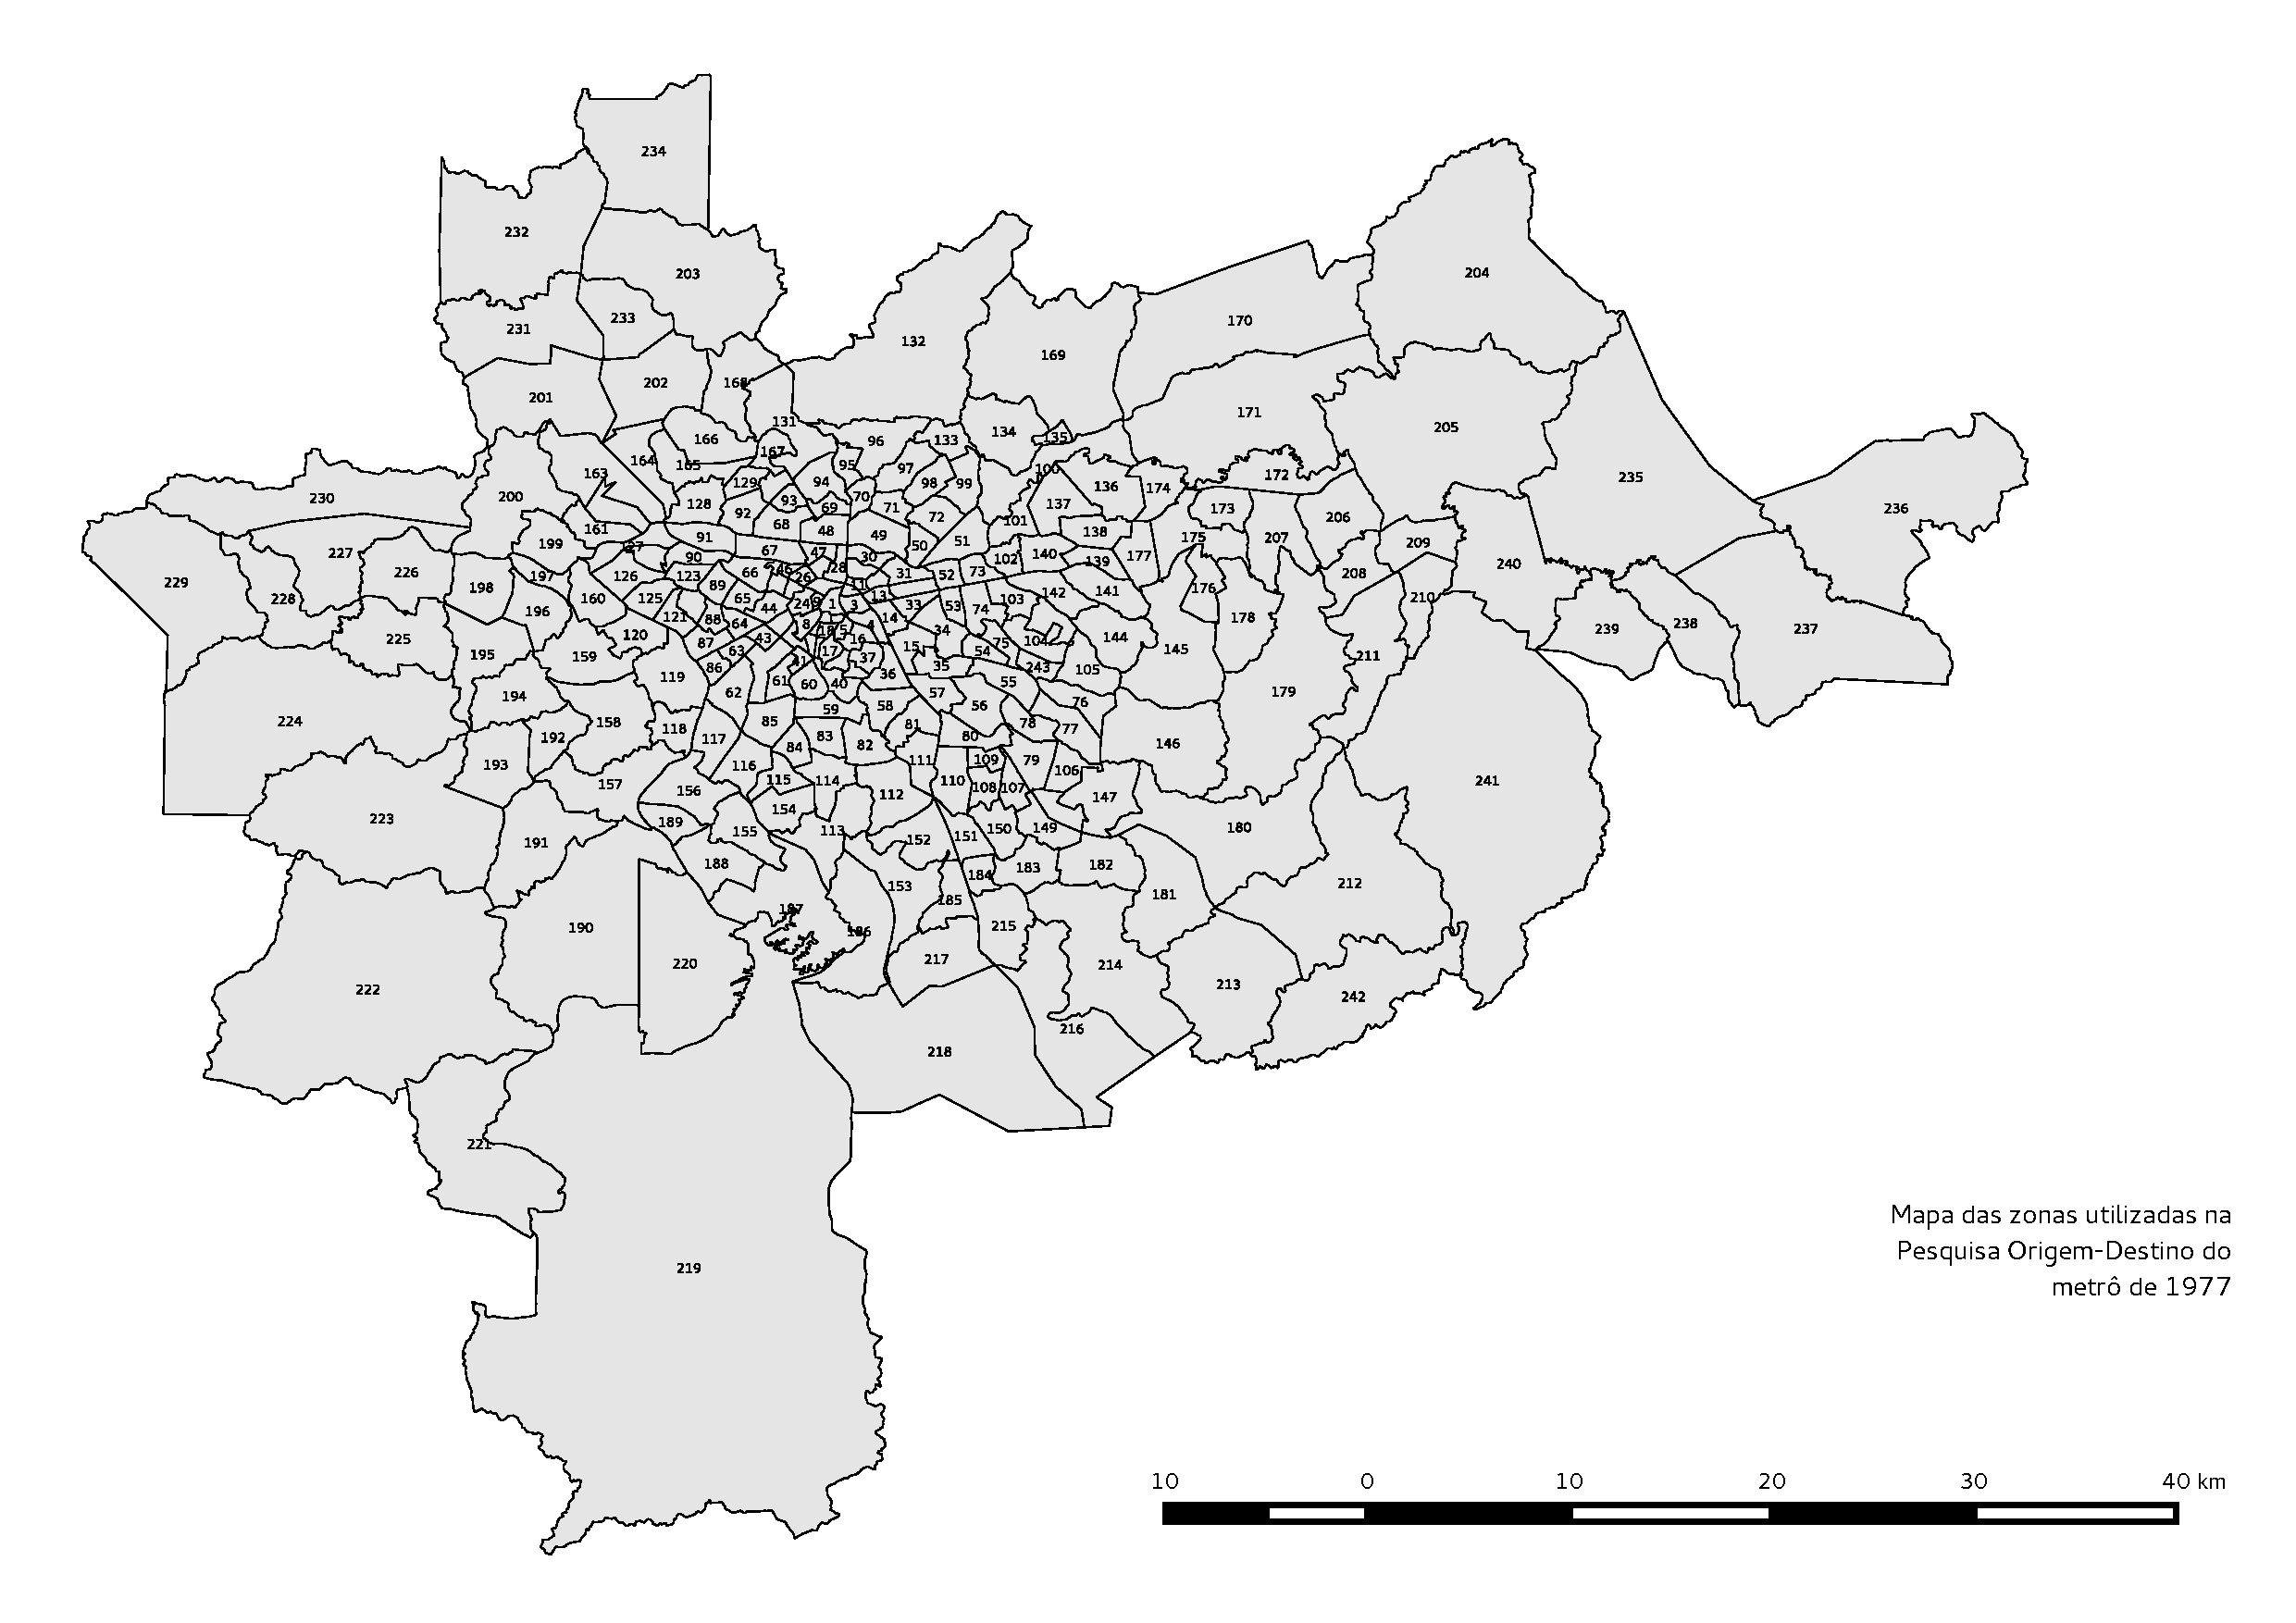
\includepdf{anexos/1977-zonas.pdf}
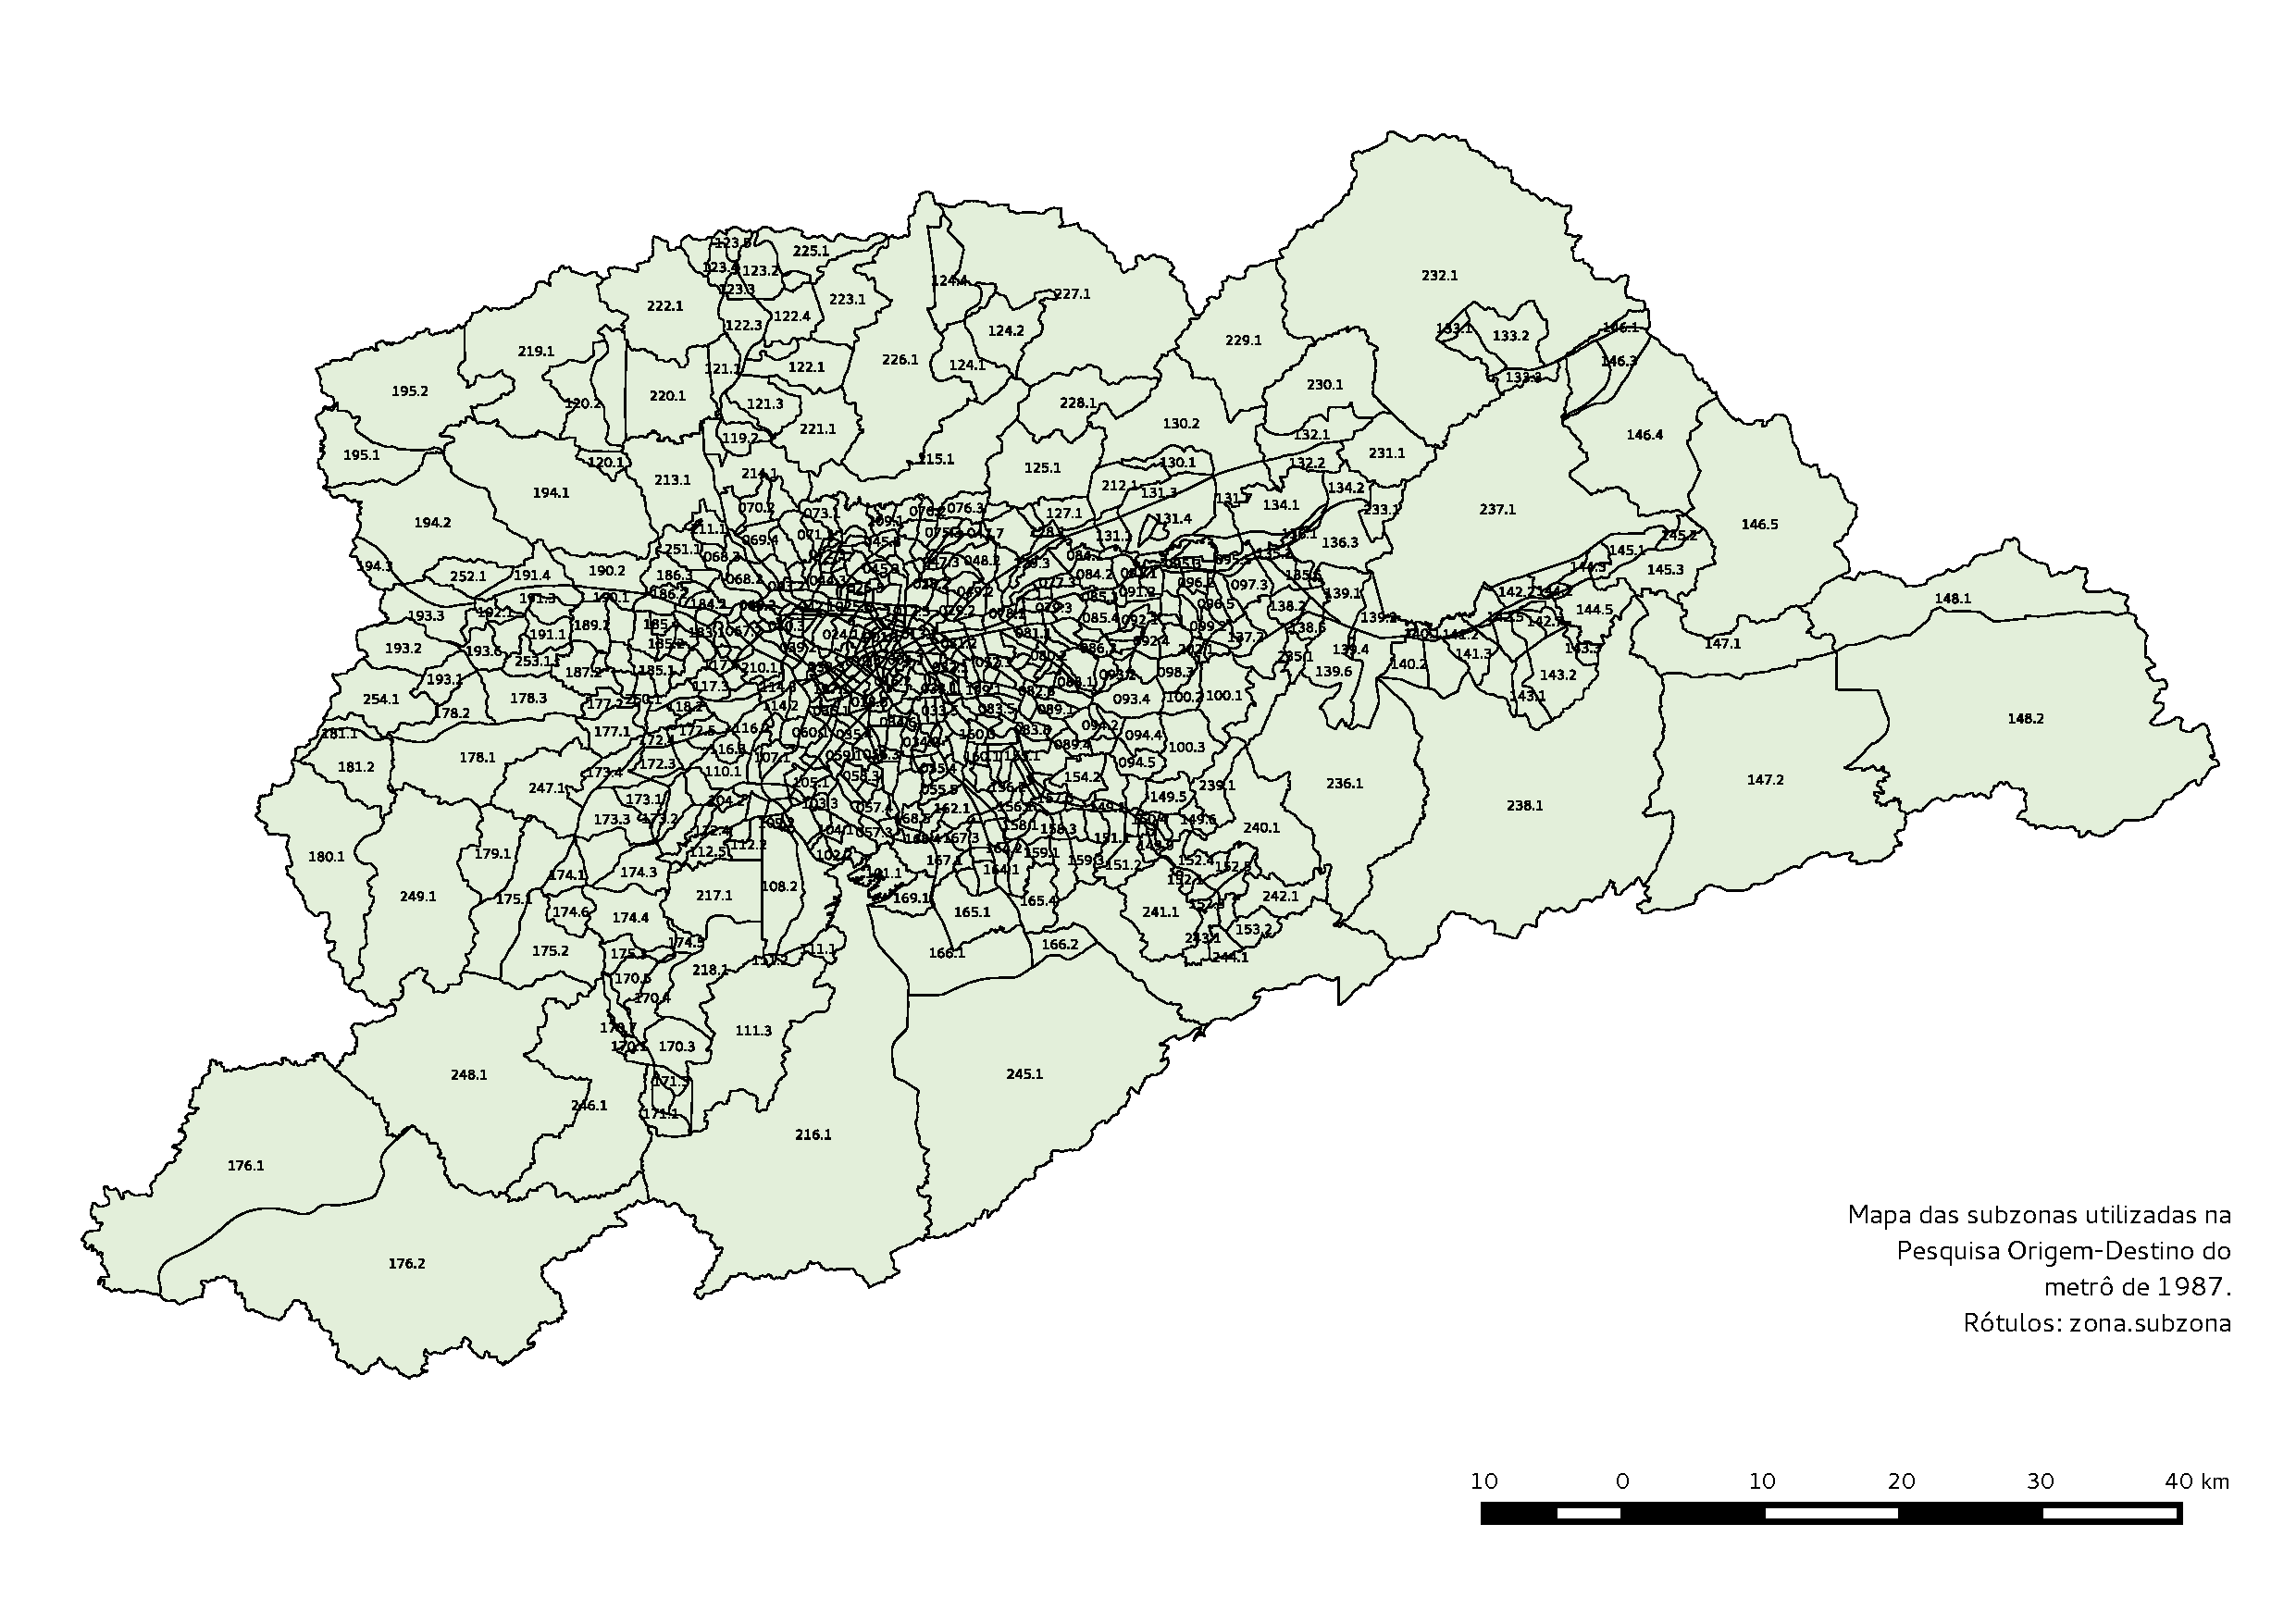
\includepdf{anexos/1987-subzonas.pdf}
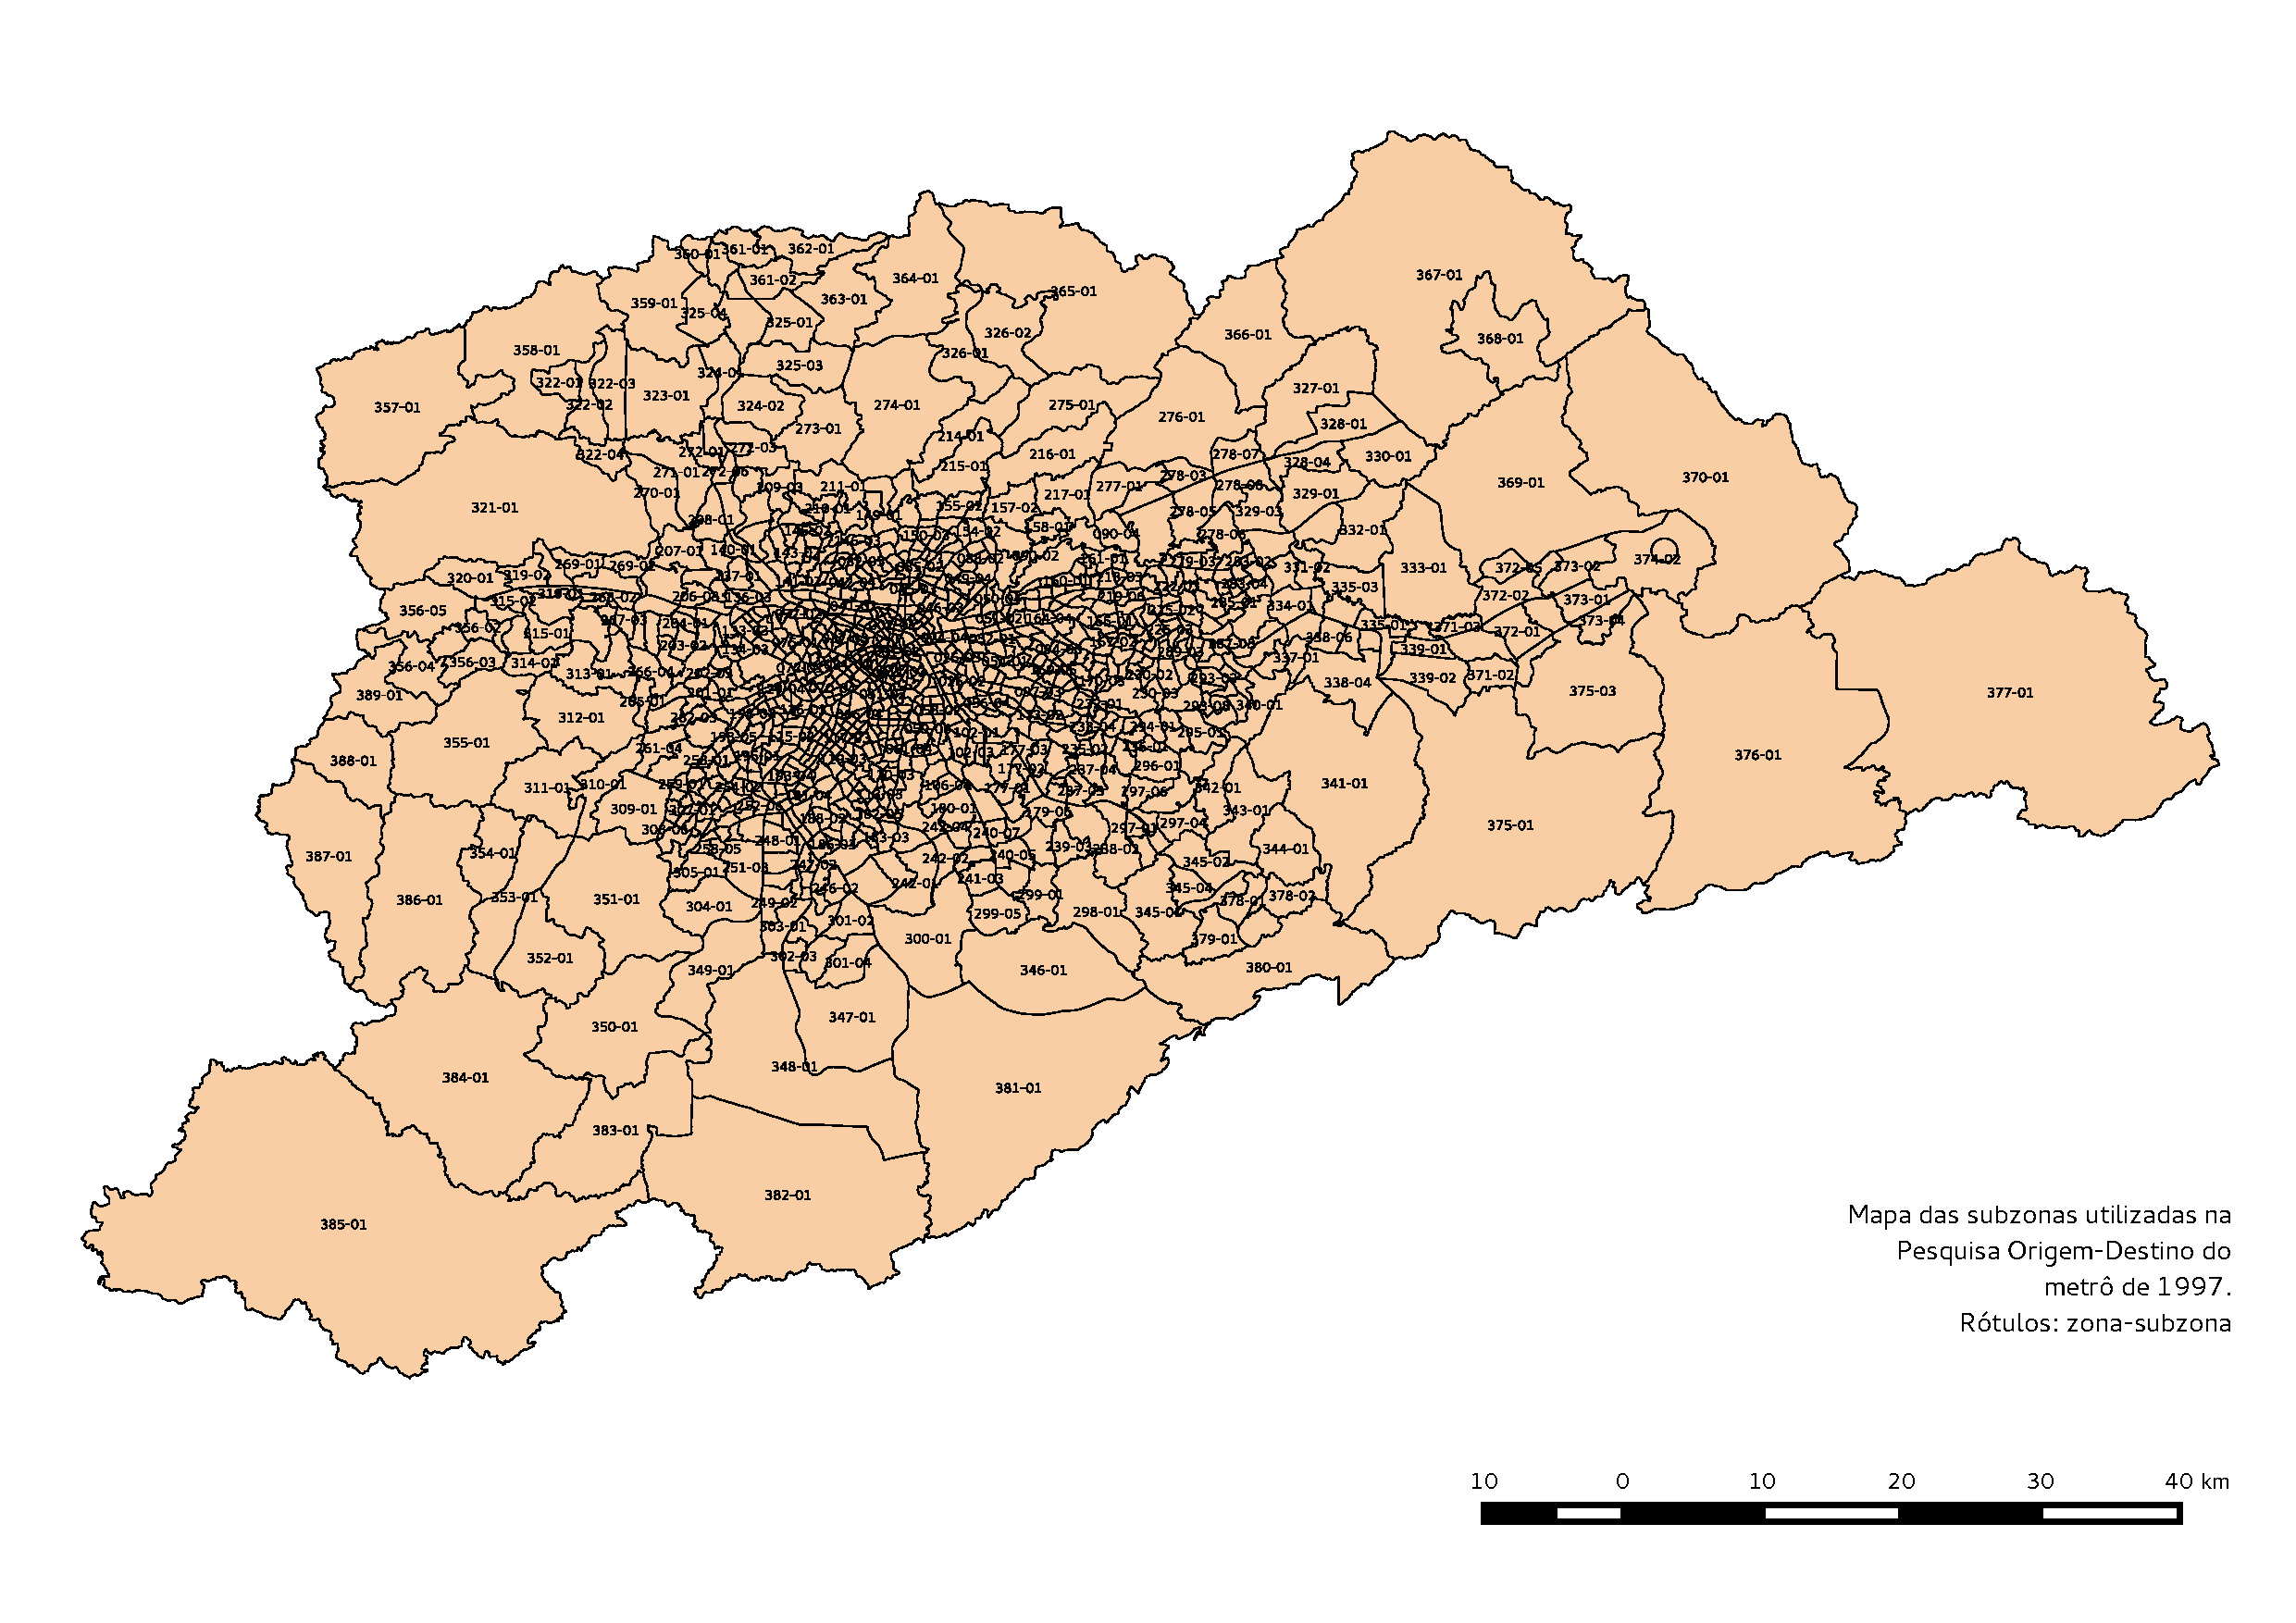
\includepdf{anexos/1997-subzonas.pdf}
%% ---
%%%%%%%%%%%%%%%%%%%%%%%%%%%%%%%%%%%%%%%%%%%
%% ---
\chapter{Layouts dos bancos de dados das Pesquisas Origem-Destino do Metrô-SP (1977, 1987, 1997 e 2007)}\label{chap:anexo_layouts}
%% ---
\includepdf[pages=-]{anexos/layout77.pdf}
\includepdf[pages=-]{anexos/layout87.pdf}
\includepdf[pages=-]{anexos/layout97.pdf}
\includepdf[pages=-]{anexos/layout07.pdf}
%% ---
%%%%%%%%%%%%%%%%%%%%%%%%%%%%%%%%%%%%%%%%%%%
%% ---
\chapter{Síntese de resultados para 4 conglomerados}\label{chap:anexo_4_clusters_td}
%% ---
\includepdf{anexos/ResumoCluster4WardCentroide.pdf}
%% ---
%%%%%%%%%%%%%%%%%%%%%%%%%%%%%%%%%%%%%%%%%%%
%% ---
\chapter{Síntese de resultados para 4 conglomerados - segmentação por ano}\label{chap:anexo_4_clusters_fam}
%% ---
\includepdf{anexos/ResumoCluster4FAMCentroide.pdf}
\includepdf{anexos/ResumoCluster4FAMCentroide2.pdf}
%% ---
%%%%%%%%%%%%%%%%%%%%%%%%%%%%%%%%%%%%%%%%%%%
%% ---
\chapter{Resultados das regressões logísticas para atributos de viagens da pessoa - todas variáveis}\label{chap:reg-log-pess}
%% ---
\includepdf[pages=-]{anexos/anexo-resultados-reg-logist.pdf}
%% ---
%%%%%%%%%%%%%%%%%%%%%%%%%%%%%%%%%%%%%%%%%%%
%% ---
\chapter{Resultados das regressões quasi-poisson}\label{chap:reg-poisson}
%% ---
\includepdf[pages=-]{anexos/resultados-reg-poisson.pdf}
\includepdf[pages=-]{anexos/resultados-reg-poisson1.pdf}
\includepdf[pages=-]{anexos/resultados-reg-poisson2.pdf}
%% ---
%%%%%%%%%%%%%%%%%%%%%%%%%%%%%%%%%%%%%%%%%%%
%% ---
\chapter{Rotinas de Preparação das Bases de Dados das Pesquisas Origem-Destino do Metrô-SP (1977, 1987, 1997 e 2007)}\label{chap:anexo_rotinas}
%% ---
\includepdf[pages=-]{anexos/rotinafinal1977.pdf}
\includepdf[pages=-]{anexos/rotinafinal1987.pdf}
\includepdf[pages=-]{anexos/rotinafinal1997.pdf}
\includepdf[pages=-]{anexos/rotinafinal2007.pdf}
%% ---
%%%%%%%%%%%%%%%%%%%%%%%%%%%%%%%%%%%%%%%%%%%
% ---
%% ---

\end{anexosenv}

%---------------------------------------------------------------------
% INDICE REMISSIVO
%---------------------------------------------------------------------
\phantompart
\printindex
%---------------------------------------------------------------------
%\listoftodos
\end{document}
